% Options for packages loaded elsewhere
\PassOptionsToPackage{unicode}{hyperref}
\PassOptionsToPackage{hyphens}{url}
\PassOptionsToPackage{dvipsnames,svgnames,x11names}{xcolor}
%
\documentclass[
]{book}
\usepackage{amsmath,amssymb}
\usepackage{lmodern}
\usepackage{iftex}
\ifPDFTeX
  \usepackage[T1]{fontenc}
  \usepackage[utf8]{inputenc}
  \usepackage{textcomp} % provide euro and other symbols
\else % if luatex or xetex
  \usepackage{unicode-math}
  \defaultfontfeatures{Scale=MatchLowercase}
  \defaultfontfeatures[\rmfamily]{Ligatures=TeX,Scale=1}
\fi
% Use upquote if available, for straight quotes in verbatim environments
\IfFileExists{upquote.sty}{\usepackage{upquote}}{}
\IfFileExists{microtype.sty}{% use microtype if available
  \usepackage[]{microtype}
  \UseMicrotypeSet[protrusion]{basicmath} % disable protrusion for tt fonts
}{}
\makeatletter
\@ifundefined{KOMAClassName}{% if non-KOMA class
  \IfFileExists{parskip.sty}{%
    \usepackage{parskip}
  }{% else
    \setlength{\parindent}{0pt}
    \setlength{\parskip}{6pt plus 2pt minus 1pt}}
}{% if KOMA class
  \KOMAoptions{parskip=half}}
\makeatother
\usepackage{xcolor}
\usepackage{color}
\usepackage{fancyvrb}
\newcommand{\VerbBar}{|}
\newcommand{\VERB}{\Verb[commandchars=\\\{\}]}
\DefineVerbatimEnvironment{Highlighting}{Verbatim}{commandchars=\\\{\}}
% Add ',fontsize=\small' for more characters per line
\usepackage{framed}
\definecolor{shadecolor}{RGB}{248,248,248}
\newenvironment{Shaded}{\begin{snugshade}}{\end{snugshade}}
\newcommand{\AlertTok}[1]{\textcolor[rgb]{0.94,0.16,0.16}{#1}}
\newcommand{\AnnotationTok}[1]{\textcolor[rgb]{0.56,0.35,0.01}{\textbf{\textit{#1}}}}
\newcommand{\AttributeTok}[1]{\textcolor[rgb]{0.77,0.63,0.00}{#1}}
\newcommand{\BaseNTok}[1]{\textcolor[rgb]{0.00,0.00,0.81}{#1}}
\newcommand{\BuiltInTok}[1]{#1}
\newcommand{\CharTok}[1]{\textcolor[rgb]{0.31,0.60,0.02}{#1}}
\newcommand{\CommentTok}[1]{\textcolor[rgb]{0.56,0.35,0.01}{\textit{#1}}}
\newcommand{\CommentVarTok}[1]{\textcolor[rgb]{0.56,0.35,0.01}{\textbf{\textit{#1}}}}
\newcommand{\ConstantTok}[1]{\textcolor[rgb]{0.00,0.00,0.00}{#1}}
\newcommand{\ControlFlowTok}[1]{\textcolor[rgb]{0.13,0.29,0.53}{\textbf{#1}}}
\newcommand{\DataTypeTok}[1]{\textcolor[rgb]{0.13,0.29,0.53}{#1}}
\newcommand{\DecValTok}[1]{\textcolor[rgb]{0.00,0.00,0.81}{#1}}
\newcommand{\DocumentationTok}[1]{\textcolor[rgb]{0.56,0.35,0.01}{\textbf{\textit{#1}}}}
\newcommand{\ErrorTok}[1]{\textcolor[rgb]{0.64,0.00,0.00}{\textbf{#1}}}
\newcommand{\ExtensionTok}[1]{#1}
\newcommand{\FloatTok}[1]{\textcolor[rgb]{0.00,0.00,0.81}{#1}}
\newcommand{\FunctionTok}[1]{\textcolor[rgb]{0.00,0.00,0.00}{#1}}
\newcommand{\ImportTok}[1]{#1}
\newcommand{\InformationTok}[1]{\textcolor[rgb]{0.56,0.35,0.01}{\textbf{\textit{#1}}}}
\newcommand{\KeywordTok}[1]{\textcolor[rgb]{0.13,0.29,0.53}{\textbf{#1}}}
\newcommand{\NormalTok}[1]{#1}
\newcommand{\OperatorTok}[1]{\textcolor[rgb]{0.81,0.36,0.00}{\textbf{#1}}}
\newcommand{\OtherTok}[1]{\textcolor[rgb]{0.56,0.35,0.01}{#1}}
\newcommand{\PreprocessorTok}[1]{\textcolor[rgb]{0.56,0.35,0.01}{\textit{#1}}}
\newcommand{\RegionMarkerTok}[1]{#1}
\newcommand{\SpecialCharTok}[1]{\textcolor[rgb]{0.00,0.00,0.00}{#1}}
\newcommand{\SpecialStringTok}[1]{\textcolor[rgb]{0.31,0.60,0.02}{#1}}
\newcommand{\StringTok}[1]{\textcolor[rgb]{0.31,0.60,0.02}{#1}}
\newcommand{\VariableTok}[1]{\textcolor[rgb]{0.00,0.00,0.00}{#1}}
\newcommand{\VerbatimStringTok}[1]{\textcolor[rgb]{0.31,0.60,0.02}{#1}}
\newcommand{\WarningTok}[1]{\textcolor[rgb]{0.56,0.35,0.01}{\textbf{\textit{#1}}}}
\usepackage{longtable,booktabs,array}
\usepackage{calc} % for calculating minipage widths
% Correct order of tables after \paragraph or \subparagraph
\usepackage{etoolbox}
\makeatletter
\patchcmd\longtable{\par}{\if@noskipsec\mbox{}\fi\par}{}{}
\makeatother
% Allow footnotes in longtable head/foot
\IfFileExists{footnotehyper.sty}{\usepackage{footnotehyper}}{\usepackage{footnote}}
\makesavenoteenv{longtable}
\usepackage{graphicx}
\makeatletter
\def\maxwidth{\ifdim\Gin@nat@width>\linewidth\linewidth\else\Gin@nat@width\fi}
\def\maxheight{\ifdim\Gin@nat@height>\textheight\textheight\else\Gin@nat@height\fi}
\makeatother
% Scale images if necessary, so that they will not overflow the page
% margins by default, and it is still possible to overwrite the defaults
% using explicit options in \includegraphics[width, height, ...]{}
\setkeys{Gin}{width=\maxwidth,height=\maxheight,keepaspectratio}
% Set default figure placement to htbp
\makeatletter
\def\fps@figure{htbp}
\makeatother
\setlength{\emergencystretch}{3em} % prevent overfull lines
\providecommand{\tightlist}{%
  \setlength{\itemsep}{0pt}\setlength{\parskip}{0pt}}
\setcounter{secnumdepth}{5}
\usepackage{booktabs}
\usepackage{amsthm}
\makeatletter
\def\thm@space@setup{%
  \thm@preskip=8pt plus 2pt minus 4pt
  \thm@postskip=\thm@preskip
}
\makeatother
\usepackage{float}
\floatplacement{figure}{H}
\renewcommand{\figurename}{Figura}
\renewcommand{\tablename}{Tabla}
\renewcommand{\contentsname}{Índice}
\renewcommand{\chaptername}{Capítulo}
\renewcommand{\bibname}{Bibliografía}

% https://tex.stackexchange.com/questions/82993/how-to-change-the-name-of-document-elements-like-figure-contents-bibliogr
\usepackage{booktabs}
\usepackage{longtable}
\usepackage{array}
\usepackage{multirow}
\usepackage{wrapfig}
\usepackage{float}
\usepackage{colortbl}
\usepackage{pdflscape}
\usepackage{tabu}
\usepackage{threeparttable}
\usepackage{threeparttablex}
\usepackage[normalem]{ulem}
\usepackage{makecell}
\usepackage{xcolor}
\ifLuaTeX
  \usepackage{selnolig}  % disable illegal ligatures
\fi
\usepackage[]{natbib}
\bibliographystyle{plainnat}
\IfFileExists{bookmark.sty}{\usepackage{bookmark}}{\usepackage{hyperref}}
\IfFileExists{xurl.sty}{\usepackage{xurl}}{} % add URL line breaks if available
\urlstyle{same} % disable monospaced font for URLs
\hypersetup{
  pdftitle={Guía para el Control de Divulgación Estadística en Microdatos},
  pdfauthor={Subdepartamento de Investigación Estadística},
  colorlinks=true,
  linkcolor={Maroon},
  filecolor={Maroon},
  citecolor={Blue},
  urlcolor={blue},
  pdfcreator={LaTeX via pandoc}}

\title{Guía para el Control de Divulgación Estadística en Microdatos}
\author{Subdepartamento de Investigación Estadística}
\date{2023-10-18}

\usepackage{amsthm}
\newtheorem{theorem}{Teorema}[chapter]
\newtheorem{lemma}{Lema}[chapter]
\newtheorem{corollary}{Corolario}[chapter]
\newtheorem{proposition}{Proposición}[chapter]
\newtheorem{conjecture}{Conjetura}[chapter]
\theoremstyle{definition}
\newtheorem{definition}{Definición}[chapter]
\theoremstyle{definition}
\newtheorem{example}{Bloque}[chapter]
\theoremstyle{definition}
\newtheorem{exercise}{Ejercicio}[chapter]
\theoremstyle{definition}
\newtheorem{hypothesis}{Hipotesis}[chapter]
\theoremstyle{remark}
\newtheorem*{remark}{Remarca}
\newtheorem*{solution}{Solución}
\begin{document}
\maketitle

{
\hypersetup{linkcolor=}
\setcounter{tocdepth}{1}
\tableofcontents
}
\hypertarget{prefacio}{%
\chapter{Prefacio}\label{prefacio}}

Los datos son un recurso valioso que proporciona información crítica para estadísticos, científicos sociales y científicos de datos. Estos datos se utilizan para generar perspectivas detalladas y oportunas que responden a las necesidades de información de una amplia gama de partes interesadas.

En un mundo donde cada vez más grandes volúmenes de datos provienen de un número creciente de proveedores, las Oficinas Nacionales de Estadística (ONE) están utilizando enfoques innovadores para mantener estándares y definiciones de datos, sistemas de gestión de privacidad y confidencialidad, e intercambio responsable de datos.

Las ONE tienen un papel de liderazgo que desempeñar en el establecimiento de formas seguras y transparentes de compartir datos, experiencias y mejores prácticas para respaldar el uso de datos con fines de prueba, evaluación, educación y desarrollo. Con la integridad y la confidencialidad de los datos a la vanguardia, las ONE están posicionandose cada vez más para proporcionar herramientas, métodos y enfoques para promover el intercambio responsable de datos, a fin de satisfacer las necesidades de un número creciente de partes interesadas en este ámbito que está en constante cambio.

Las ONE reconocen que se debe cumplir con el llamado a una mayor apertura y transparencia de los datos. Sin embargo, también se comprometen a proteger la confidencialidad y la privacidad integradas en sus tenencias de datos.

Se reconoce ampliamente que la difusión de información que es a la vez útil y completamente segura, no puede lograrse en su totalidad. Por lo tanto, la seguridad es un concepto relativo, no absoluto, y se debe entender como una métrica, no un estado.

Es dentro de este contexto que las ONE deben establecer protocolos para la difusión segura de datos y métricas para medir la utilidad de la información estadística publicada y el grado de protección de las unidades, ya sean personas naturales o jurídicas, e información recopilada de la cual se deriva.

Esta guía es para aquellos que trabajan en una ONE u oficina estatal que están involucrados en la gestión del acceso a datos estadísticos, y que deseen explorar herramientas de protección de datos para que los usuarios accedan a ellos. La guía destaca algunas aplicaciones exitosas recientes de control a la divulgación estadística en microdatos en el Instituto Nacional de Estadísticas de Chile (INE), y presenta un marco general sobre medición y evaluación de riesgos, técnicas para generar datos anonimizados, y sobre las medidas de utilidad que se pueden usar para evaluar qué tan bien los datos anonimizados satisfacen las necesidades analíticas de los usuarios. La guía también incluye recomendaciones sobre qué enfoques utilizar en diferentes situaciones, así como consejos prácticos y recursos para que los profesionales comiencen su experiencia en la implementación de proceso de control a la divulgación estadística.

Esta guía se basa en Statistical Disclosure Control: A Practice Guide \citet{benschop2019statistical} y en la \href{https://www.ine.gob.cl/docs/default-source/buenas-practicas/directrices-metodologicas/guias-y-orientaciones-metodologicas/documentos/gu\%C3\%ADa-control-divulgaci\%C3\%B3n-estad\%C3\%ADstica-microdatos.pdf?sfvrsn=b6bdd28f_2}{Guía para el control de divulgación estadística en microdatos}, elaborada por el INE en 2021, que es el primer esfuerzo en esta materia en instituciones del Estado en Chile. Sin embargo, aún puede enriquecerse a partir de nuevos conocimientos y experiencias que tanto investigadores como profesionales puedan aportar.

¡Esperamos que esta guía lo ayude en su viaje hacia la implementación de procesos de control a la divulgación estadística en su organización!

\hypertarget{autores-de-esta-guuxeda}{%
\section{Autores de esta guía}\label{autores-de-esta-guuxeda}}

\begin{itemize}
\item
  \textbf{Jonathan González Mejías}, Subdepartamento de Estadísticas Socioeconómicas, Subdirección Técnica en Instituto Nacional de Estadísticas de Chile.
\item
  \textbf{José Bustos Melo}, Subdepartamento de Investigación Estadística, Departamento de Metodologías e Innovación Estadística en Instituto Nacional de Estadísticas de Chile.
\item
  \textbf{Julio Guerrero Rojas}, Subdepartamento de Investigación Estadística, Departamento de Metodologías e Innovación Estadística en Instituto Nacional de Estadísticas de Chile.
\item
  \textbf{Lissette Bastías Navarro}, Subdepartamento de Calidad y Estándares, Departamento de Metodologías e Innovación Estadística en Instituto Nacional de Estadísticas de Chile.
\item
  \textbf{Nicolás Berhó Montalvo}, Subdepartamento de Estadísticas de Condiciones de Vida, Subdirección Técnica en Instituto Nacional de Estadísticas de Chile.
\end{itemize}

\hypertarget{reconocimientos}{%
\section{Reconocimientos}\label{reconocimientos}}

Este proyecto conjunto es un testimonio del esfuerzo colaborativo que comenzó a gestarse a finales de 2019, en el cual participaron activamente los analistas de la Subdirección Técnica (SDT) y del Departamento de Metodologías e Innovación Estadística (DMIE). Durante esta travesía, se realizaron reuniones estratégicas que permitieron explorar y analizar las diversas formas de anonimización históricamente empleadas por nuestros equipos. Estas discusiones fueron fundamentales para identificar puntos comunes y optimizar nuestros esfuerzos, evitando la duplicación de tareas y enfocando nuestros recursos de manera eficiente.

La coordinación y organización de este arduo trabajo estuvieron a cargo del DMIE, bajo la hábil dirección de Denisse López. Reconocemos su liderazgo y dedicación en la conducción de este proyecto.

Este logro no habría sido posible sin la valiosa colaboración de cada persona involucrada en el proceso, ya sea de forma directa o indirecta. Valoramos y agradecemos profundamente a todos los miembros del equipo y a nuestro Instituto Nacional de Estadísticas (INE) en su conjunto. Sin duda, este es un esfuerzo colectivo que fortalece nuestra institución y enriquece nuestro compromiso con la excelencia en estadísticas.

Aunque no es posible mencionar a cada analista en particular, queremos expresar nuestra sincera gratitud a todos aquellos que aportaron su tiempo, conocimientos y dedicación para hacer de este proyecto una realidad. Cada contribución, por pequeña que parezca, ha sido fundamental en la consecución de este importante trabajo. Juntos, hemos construido un proyecto sólido que nos impulsa hacia adelante en nuestra misión de generar datos precisos y relevantes para nuestra sociedad.

Nuestro agradecimiento se extiende a cada uno de ustedes y a todas las personas que, de una u otra manera, han contribuido a este proyecto. Su esfuerzo y colaboración han sido esenciales y apreciadas en todo momento. Seguimos comprometidos con nuestra labor y esperamos seguir trabajando juntos en futuros proyectos que beneficien a nuestra institución y a la comunidad en general.

\hypertarget{introducciuxf3n}{%
\chapter{Introducción}\label{introducciuxf3n}}

Como Instituto Nacional de Estadística (en adelante, INE) tenemos la responsabilidad de la recopilación y difusión de estadísticas oficiales, tomando resguardos para cumplir con la Ley de Secreto Estadístico (Art.29, Ley 17.374 \citep{ley1970}), la Ley sobre Protección de la Vida Privada (Art.2e, Ley 19.628 \citep{ley1999}) y la legislación propia de las entidades públicas, todas en la línea de la protección y privacidad de la información difundida. Por otro lado, a nivel país, en los últimos años, ha existido un aumento constante en transparentar y disponer información tanto a nivel privado como público, mediante la ``ley de transparencia'' (Ley 20.285 \citep{ley2008}), promulgada en año 2008.

Es en esta misma línea que las Naciones Unidas también abogan por la libre difusión de los microdatos. Lo que permite a los usuarios contribuir con investigación, aumenta la transparencia y la responsabilidad de los institutos nacionales de estadística y permite mejoras en la calidad a través de la retroalimentación de los usuarios \citep{nacionesunidas}.

En paralelo la comunidad estadística ha reconocido la importancia de asegurar la información para mantener la confianza de las poblaciones a las que servimos. En este sentido, el Código Nacional de Buenas Prácticas Estadísticas del INE, en su principio 4 sobre confidencialidad estadística, establece que el ``INE y los demás miembros del Sistema Estadístico Nacional (SEN) deben garantizar la protección y confidencialidad de la información con la que se producen las estadísticas oficiales, así como evitar la identificación de las fuentes'' \citep{institutonacionaldeestadisticas2015}.

Los principios en competencia de la seguridad de los datos y la difusión de microdatos se someten a arbitraje a través de un dominio de estadísticas llamado Control de Divulgación Estadística (SDC, por su sigla en inglés). Los métodos SDC permiten proteger un conjunto de datos mediante la aplicación de herramientas estadísticas, lo que posibilita a la institución difundir de manera segura el conjunto de datos.

La experiencia del INE en términos de control de divulgación estadística ha ido avanzando, iniciando en junio del año 2009, bajo la Resolución exenta N° 1918, emitida en Santiago el 10 de junio de 2009, expone acerca de una experiencia localizada, sobre el tratamiento que se buscaba dar a datos económicos, luego en 2019, un equipo multidisciplinario de la producción estadística institucional, define los lineamientos para desarrollar un proceso estandarizado de control de divulgación en las operaciones estadísticas que desarrolla el INE, entregando como resultado una primera versión de la ``Guía para el control de divulgación estadística en microdatos''. En diciembre del 2021 se transforma en un estándar institucional disponible en la página web institucional \url{https://www.ine.gob.cl/calidad-estadistica/directrices-metodologicas} \citep{institutonacionaldeestadisticas2021}.

Este documento exige normar el subproceso de control a la divulgación estadística o anonimización, a fin de responder de manera adecuada, oportuna y segura a los usuarios que requieren información de interés y que solicitan las bases de microdatos, al mismo tiempo de tener procedimientos estandarizados en la producción de estadísticas oficiales.

Esta guía busca brindar pasos prácticos bajo lineamientos institucionales para aquellas operaciones estadísticas que requieran desbloquear el acceso a sus datos de manera segura y garantizar que los datos sigan siendo aptos para su propósito.

\hypertarget{estableciendo-una-base-de-conocimiento}{%
\section{Estableciendo una base de conocimiento}\label{estableciendo-una-base-de-conocimiento}}

La publicación de datos es importante, ya que permite a los investigadores y responsables políticos replicar los resultados publicados oficialmente, generar nuevos conocimientos sobre los problemas, evitar la duplicación de encuestas y proporcionar mayores retornos a la inversión en el proceso de encuesta.

Tanto la producción de informes, con tablas agregadas de indicadores y estadísticas, como la publicación de microdatos resultan en desafíos de privacidad para el productor. En el pasado, para muchas ONE, el único requisito era publicar un informe y algunos indicadores clave. El reciente movimiento en torno a los datos abiertos, el gobierno abierto y la transparencia significa que las ONE están bajo una mayor presión para liberar sus microdatos, para permitir un uso más amplio de los datos recopilados a través de fondos públicos. Esta guía se centra en los métodos y procesos para la liberación de microdatos, ya sea que estos provengan de encuestas, censos o registros estadísticos generados por el INE. Por tanto, el alcance de los procesos que se describen en esta guía se ciñe a proveer directriz circunscrita al campo de los microdatos, por lo que se excluyen los procesos de control de divulgación estadística orientados a tabulados, estadísticas geoespaciales, publicaciones web o visualizaciones de mapas, etc., que requieren enfoques diferentes al propuesto en esta guía. Asimismo, se distingue la necesidad de establecer lineamientos para el control de divulgación estadística en la publicación de tablas y publicaciones web, con el fin de cubrir más ámbitos de la producción estadística del INE.

Se requiere la difusión de datos de manera segura para proteger la integridad del sistema estadístico, al garantizar que el INE cumpla con su compromiso con los encuestados de proteger su identidad. Las ONE no comparten ampliamente, en detalle sustancial, su conocimiento y experiencia usando SDC y los procesos para crear datos seguros con otras ONE. Esto lo hace difícil para las instituciones nuevas en el proceso para implementar soluciones. Para llenar esta brecha de experiencia y conocimiento, el equipo de la mesa de trabajo INE (en adelante mesa) evaluó el uso de un amplio conjunto de métodos de SDC en una gama de microdatos de encuestas que cubren importantes temas de desarrollo relacionados con trabajo, seguridad ciudadana, empresas de ferrocarriles, trámites de circulación. Dado que sus productores ya habían tratado estos datos, no era posible, ni era objetivo de la mesa, emitir un juicio sobre la seguridad de estos datos, los cuales son de dominio público. El enfoque se centró más bien en medir los efectos que varios de los métodos tendrían que ver con la relación riesgo -- utilidad para los microdatos producidos para medir indicadores comunes de desarrollo. La experiencia de esta experimentación es útil para informar la discusión de los procesos y métodos en esta guía.

\hypertarget{propuxf3sito-de-esta-guuxeda}{%
\section{Propósito de esta guía}\label{propuxf3sito-de-esta-guuxeda}}

Esta guía tiene como propósito presentar los lineamientos para la aplicación del control de divulgación estadística en microdatos derivados de censos, registros estadísticos y encuestas por muestreo desarrollados por el INE, permitiendo establecer qué microdatos pueden ser liberados y bajo qué condiciones.

Esta guía no pretende prescribir o abogar por cambios en los métodos que los productores de datos específicos ya están utilizando y que han diseñado para ajustarse y cumplir con sus políticas de difusión de datos existentes, empero, ordenarlos. Los métodos discutidos en esta guía provienen de una gran cantidad de literatura sobre SDC. Los procesos que subyacen a muchos de los métodos son objeto de una extensa investigación académica y muchos, si no todos, son utilizados ampliamente por ONE con experiencia en la preparación de microdatos para su publicación.

Siempre que sea posible, para cada método y tema, se proporciona ejemplos elaborados, referencias al trabajo original o seminal que describe los métodos y algoritmos en detalle y las lecturas recomendadas. Esto, cuando se combina con la discusión del método y las consideraciones prácticas en esta guía, debería permitir al lector comprender los métodos y sus fortalezas y debilidades. También proporciona suficientes detalles para que los lectores usen una solución de \emph{software} adecuada para implementar los métodos.

Para los ejercicios de esta guía, se ha utilizado el paquete de código abierto y gratuito para SDC llamado \texttt{sdcMicro}, así como el lenguaje y entorno de programación estadístico \texttt{R}. \texttt{sdcMicro} es un paquete adicional para el lenguaje \texttt{R}. El paquete fue desarrollado y es mantenido por Matthias Templ, Alexander Kowarik y Bernhard Meindl\protect\hyperlink{_ftn1}{{[}1{]}}. El lenguaje estadístico \texttt{R} y el paquete \texttt{sdcMicro}, así como cualquier otro paquete necesario para el proceso SDC, están disponibles gratuitamente en los \texttt{mirrors} de la Red Integral de Archivos \texttt{R} (CRAN\protect\hyperlink{_ftn2}{{[}2{]}}) (\url{http://cran.r-project.org}/). El lenguaje está disponible para los sistemas operativos Linux, Windows y Macintosh. Se ha elegido usar \texttt{R} y \texttt{sdcMicro} porque está disponible gratuitamente, admite todos los formatos de datos principales y es fácil de adaptar por el usuario. El Banco Mundial, a través de IHSN\protect\hyperlink{_ftn3}{{[}3{]}}, también ha proporcionado fondos para el desarrollo del paquete \texttt{sdcMicro} para garantizar que cumpla con los requisitos de las ONE.

Esta guía no proporciona una revisión de todos los demás paquetes disponibles para implementar el proceso SDC, pues se trata más de proporcionar información práctica sobre la aplicación de los métodos. Sin embargo, cabe destacar otro paquete de \emph{software} en particular que las ONE utilizan comúnmente: \texttt{𝜇-ARGUS}\protect\hyperlink{_ftn4}{{[}4{]}}. \texttt{𝜇-ARGUS} es desarrollado por Statistics Netherlands. \texttt{sdcMicro} y \texttt{𝜇-ARGUS} son ampliamente utilizados en oficinas de estadística en la Unión Europea e implementan muchos de los mismos métodos.

Las necesidades de usuario acerca de algún conocimiento de \texttt{R} para usar \texttt{sdcMicro} está más allá del alcance de esta guía, así como enseñar el uso de \texttt{R}, pero se presenta una serie de estudios de casos que incluyen el código para el anonimato de una serie de conjuntos de datos de demostración con \texttt{R}. A través de estos estudios de caso, se demuestra una serie de enfoques para el proceso de anonimización en \texttt{R}.

\hypertarget{esquema-de-esta-guuxeda}{%
\section{Esquema de esta guía}\label{esquema-de-esta-guuxeda}}

Esta guía está dividida en las siguientes secciones principales:

\begin{enumerate}
\def\labelenumi{\arabic{enumi}.}
\item
  \textbf{Introducción a sdcMicro}: donde se visualiza la necesidad de aplicar los métodos SDC y el trade off que se produce entre el riesgo versus la utilidad.
\item
  \textbf{Tipos de liberación de datos}: en este apartado encontrarán los tres tipos de métodos de divulgación, archivos de uso público (PUF, por sus siglas en inglés), archivos de uso científico (SUF, por sus siglas en inglés) y microdatos disponibles en un centro de datos de investigación controlado.
\item
  \textbf{Medición de riesgos}: las medidas de riesgo que se utilizan y la determinación si un archivo de datos es lo suficientemente seguro para su divulgación.
\item
  \textbf{Métodos SDC}: una descripción de los métodos más utilizados para anonimizar.
\item
  \textbf{Medición de utilidad y pérdida de información}: en este apartado se profundiza acerca del trade off entre la medición de la utilidad y la pérdida de información.
\item
  \textbf{Procesos SDC INE 2021}: caso práctico implementado en el INE en la mesa de anonimización institucional.
\item
  \textbf{Caso de estudio: Enusc}: caso práctico para aplicar el método SDC en la Encuesta Nacional Urbana de Seguridad Ciudadana (ENUSC) con datos sintéticos.
\end{enumerate}

\protect\hyperlink{_ftnref1}{{[}1{]}} Matthias Templ, Alexander Kowarik, Bernhard Meindl (2015). Statistical Disclosure Control for Micro-Data Using the R Package sdcMicro. Journal of Statistical Software 67 (October): 1--36. \url{https://doi.org/10.18637/jss.v067.i04.}

\protect\hyperlink{_ftnref2}{{[}2{]}} En inglés, Comprehensive R Archive Network.

\protect\hyperlink{_ftnref3}{{[}3{]}} En inglés, International Household Survey Network.

\protect\hyperlink{_ftnref4}{{[}4{]}} \(\mu\)- ARGUS está disponible en: \url{https://research.cbs.nl/casc/mu.htm}

\hypertarget{acruxf3nimos-y-glosario}{%
\chapter{Acrónimos y glosario}\label{acruxf3nimos-y-glosario}}

\hypertarget{acruxf3nimos}{%
\section{Acrónimos}\label{acruxf3nimos}}

\begin{table}

\caption{\label{tab:tabAcron1}Lista de acrónimos}
\centering
\begin{tabular}[t]{l|l}
\hline
Acrónimo & Descripción\\
\hline
AEPD & Agencia Española de Protección de Datos\\
\hline
Bloque & Trozo de código en R que permite cargar y procesar datos, realizar los análisis estadísticos e imprimir los resultados\\
\hline
CEPAL & Comisión Económica para América Latina y el Caribe\\
\hline
DANE & Departamento Administrativo Nacional de Estadística\\
\hline
ENUSC & Encuesta Nacional Urbana de Seguridad Ciudadana\\
\hline
FCYTE & Fundación Española de Ciencia y Tecnología\\
\hline
GSBPM [1] & Modelo Genérico del Proceso Estadístico\\
\hline
IHSN [2] & Red Internacional de Encuestas de Hogares\\
\hline
INE & Instituto Nacional de Estadísticas\\
\hline
INEGI & Instituto Nacional de Estadística y Geografía\\
\hline
MINSEGPRES & Ministerio Secretaría General de la Presidencia\\
\hline
OCDE & Organización para la Cooperación y el Desarrollo Económicos\\
\hline
ONE & Oficina Nacional de Estadística\\
\hline
PITEC & Panel de Innovación tecnológica\\
\hline
PRAM [3] & Método de Post-Aleatorización\\
\hline
PUF [4] & Archivo de Uso Público\\
\hline
RUT & Rol Único Tributario\\
\hline
ROL & Identifica a una propiedad o bien raíz\\
\hline
SEN & Sistema Estadístico Nacional\\
\hline
SDC [5] & Control de Divulgación Estadística\\
\hline
sdcMicro & Paquete de implementación bajo el *software* R\\
\hline
STATCAN [6] & Estadísticas de Canadá\\
\hline
SUF [7] & Archivo de Uso Científico\\
\hline
UNECE [8] & Comisión Económica de las Naciones Unidas para Europa\\
\hline
\end{tabular}
\end{table}

{[}1{]} En inglés, \emph{Generic Statistical Business Process Model}.\\
{[}2{]} En inglés, \emph{International Household Survey Network}.\\
{[}3{]} En inglés, \emph{Post Randomization Method}.\\
{[}4{]} En inglés, \emph{Public Use File}.\\
{[}5{]} En inglés, \emph{Statistical Disclosure Control}.\\
{[}6{]} En inglés, \emph{Statistics Canada}.\\
{[}7{]} En inglés, \emph{Scientific Use File}.\\
{[}8{]} En inglés, \emph{United Nations Economic Commission for Europe}.

\hypertarget{glosario}{%
\section{Glosario}\label{glosario}}

Respecto a los términos, conceptos o categorías utilizadas en esta guía se detallan aquellos que son relevantes para la comprensión del subproceso.

\begin{table}

\caption{\label{tab:unnamed-chunk-1}Glosario de términos y conceptos}
\begin{tabu} to \linewidth {>{\raggedright}X>{\raggedright}X>{\raggedright}X}
\hline
Término & Definición & Referencia\\
\hline
\textbf{Adición de ruido} & Método basado en agregar o multiplicar un número aleatorio a los valores originales para proteger los datos de la coincidencia exacta con archivos externos. La adición de ruido se aplica típicamente a variables continuas. & [@benschop2021], pág. 9\\
\hline
\textbf{Anonimización} & Proceso técnico que consiste en transformar los datos individuales de las unidades de observación, de tal modo que no sea posible identificar sujetos o características individuales de la fuente de información, preservando así las propiedades estadísticas en los resultados. & [@institutonacionaldeestadisticas2022]\\
\hline
\textbf{Archivo de datos para uso científico} & Archivo de uso científico (SUF, por su sigla en inglés, Scientific Use File), es un tipo de publicación del archivo de microdatos, que solo está disponible para investigadores seleccionados bajo un acuerdo. También conocido como “archivo con licencia”, “microdatos bajo contrato” o “archivo de investigación”. & [@benschop2021], pág. 10\\
\hline
\textbf{Archivo de datos para uso en centro de datos de investigación controlado o enclave} & Son los archivos que pueden ofrecerse a los usuarios bajo condiciones estrictas en un enclave de datos. Se trata de una sala equipada con computadores que no están conectados a Internet ni a una red externa, y del que no se puede descargar información a través de puertos USB u otras unidades. Los enclaves de datos contienen datos que son particularmente sensibles o permiten la identificación directa o fácil de los informantes. Los ejemplos incluyen conjuntos de datos completos de censos de población, encuestas empresariales, etc. & Adaptado de [@benschop2021], pág. 20\\
\hline
\textbf{Archivo de datos para uso público} & Archivo de uso público (PUF, por sus siglas en inglés, Public Use File), es un tipo de publicación del archivo de microdatos, que está disponible gratuitamente para cualquier usuario, por ejemplo, en el sitio web del INE. & [@benschop2021], pág. 10\\
\hline
\textbf{Barajado (En inglés, shuffling)} & Método que consiste en enmascarar una variable considerada confidencial mediante la generación de una distribución condicional. & [@benschop2021], pág. 74\\
\hline
\textbf{Base de datos} & Una colección lógica de información que está interrelacionada y que se gestiona y almacena como una unidad, por ejemplo, en el mismo archivo informático. & [@oecd]\\
\hline
\textbf{Celdas confidenciales} & Las celdas de una tabla que no son publicables debido al riesgo de divulgación estadística se denominan celdas confidenciales. & [@oecd]\\
\hline
\textbf{Clave} & Combinación o patrón de variables clave o cuasi – identificadores. También, es usado el término llave. & [@benschop2021], pág. 9\\
\hline
\textbf{Codificación superior o inferior} & Corresponde a la agrupación de una variable continua en una categoría en los extremos de los valores posibles que agrupa todos los valores mayores o menores a un número (por ejemplo: valores mayores o iguales a 5 quedarán en la categoría “5 o más” mientras que el resto conserva su valor). & Adaptado de [@benschop2021], pág. 52\\
\hline
\textbf{Confidencialidad de los datos} & Es una propiedad de los datos, generalmente como resultado de medidas legislativas, que previenen su divulgación no autorizada. & [@oecd]\\
\hline
\textbf{Control de Divulgación Estadística (SDC)} & Proceso que busca tratar y alterar los datos para que puedan publicarse o difundirse sin revelar la información confidencial que contiene, mientras que, al mismo tiempo, limitan la pérdida de información debido al anonimato de los datos. En el GSBPM, estos métodos están relacionados con la etapa de difusión y generalmente se basan en restringir la cantidad o modificar los datos publicados. & [@australianbureauofstatistics2021]\\
\hline
Convenio & Contrato, convención o acuerdo que se desarrolla en función de un asunto específico destinado a crear, transferir, modificar o extinguir una obligación.
- Es un acuerdo de voluntades entre dos o más organismos públicos con personalidad jurídica, sobre cualquier cuestión pendiente de resolver.
- Son instrumentos jurídicos, suscritos por dos o más organismos de la Administración del Estado, que tienen por finalidad, comprometer la colaboración mutua entre ellos, dentro de las facultades que la ley les confiere para satisfacer necesidades actuales o futuras y que requieren de su formalización, mediante actos administrativos, para producir efectos jurídicos.
Tipos de convenios:
1. Marco: establece las bases para el intercambio de información, mediante convenios específicos.
\textbf{2. Específico: consiste en la materialización de un convenio marco, y tiene por objeto señalar específicamente las obligaciones de cada parte, detallando los compromisos que adquiere cada institución.} & Fiscalía INE\\
\hline
\textbf{Datos personales} & Son datos de carácter personal o datos personales, “los relativos a cualquier información concerniente a personas naturales, identificadas o identificables”. & [Ley N° 19628 1999]\\
\hline
\textbf{Datos originales} & Datos a los que no se les aplica algún método de anonimización. También se denominan “datos brutos” o “datos no tratados”. & [@benschop2021], pág. 11\\
\hline
\textbf{Divulgación} & Se produce cuando una persona u organización reconoce o aprende algo que no sabía sobre otra persona u organización a través de los datos divulgados. Ver también Divulgación de identidad, Divulgación de atributos y Divulgación inferencial. & [@benschop2021], pág. 9\\
\hline
\textbf{Divulgación de atributos} & La divulgación de atributos ocurre cuando un usuario puede determinar nuevas características de un individuo u organización con base en la información disponible en los datos publicados. A este usuario se le denominará intruso, ver intruso. & [@benschop2021], pág. 8\\
\hline
\textbf{Divulgación de identidad} & La divulgación de identidad ocurre cuando un intruso asocia a un individuo (o grupo) u organización conocida, con un registro de datos publicado. & [@benschop2021], pág. 9\\
\hline
\textbf{Divulgación inferencial} & La divulgación inferencial ocurre si un intruso puede determinar, a partir de los datos publicados, el valor de alguna característica de un individuo u organización con mayor precisión que lo pretendido. & [@benschop2021], pág. 9\\
\hline
\textbf{Encuesta} & Investigación sobre las características de una población particular, que utiliza procedimientos estandarizados para recopilar información de la población de estudio (incluidos censos, encuestas de muestra, la recopilación de datos de registros administrativos y actividades estadísticas derivadas) para estimar sus características mediante el uso sistemático de la metodología estadística. & [@institutonacionaldeestadisticas2022]\\
\hline
\textbf{Escenario de divulgación} & Describe la información potencialmente disponible para un tercero (por ejemplo: datos del censo, padrones electorales, registro de población, datos recopilados por empresas privadas o incluso datos de encuestas publicadas por el INE), para identificar a los encuestados y las formas en que dicha información se puede combinar con los microdatos establecidos para ser publicados y utilizados para la re-identificación de registros en el conjunto de datos. & [@benschop2021], págs. 25-26\\
\hline
\textbf{Estructura jerárquica} & Datos que se componen de colecciones de registros que están interconectados a través de enlaces, por ejemplo, individuos que pertenecen a grupos/hogares o empleados que pertenecen a empresas. & [@benschop2021], pág. 9\\
\hline
\textbf{Identificador} & Variable/información (o grupo de variables) que puede utilizarse para establecer la identidad de un individuo u organización. Los identificadores pueden conducir a una identificación directa o indirecta. & [@benschop2021], pág. 9\\
\hline
\textbf{Identificadores directos} & Son variables que identifican inequívocamente unidades estadísticas, como, RUT, ROL, número de seguro social, o nombres y direcciones de empresas o personas. Los identificadores directos deben eliminarse como primer paso del proceso de anonimización. & [@benschop2021], pág. 9\\
\hline
\textbf{Identificadores indirectos} & Son variables que, si bien no identifican inequívocamente unidades estadísticas, en combinación se pueden vincular a información externa para re-identificar a los informantes en el conjunto de datos publicado. También se les denomina “cuasi-identificadores” o “variables clave”. & [@benschop2021], pág. 9\\
\hline
\textbf{Informante} & Empresas, autoridades, personas individuales, etc., de quienes se recopilan datos e información asociada para su uso en la compilación de estadísticas. & Adaptado de [@oecd]\\
\hline
\textbf{Intervalo} & Un conjunto de números entre dos cotas designadas que pueden o no estar incluidos (abiertos, semiabiertos o cerrados). Los corchetes (por ejemplo, [0, 1]) denotan un intervalo cerrado, que incluye los puntos finales 0 y 1. Los paréntesis, por ejemplo, (0, 1) denotan un intervalo abierto, que no incluye los puntos finales. & Adaptado de [@benschop2021], pág. 9\\
\hline
\textbf{Intruso} & Usuario que hace mal uso de los datos publicados al tratar de identificar y divulgar información sobre un individuo u organización, utilizando un conjunto de características conocidas por el usuario. & [@benschop2021], pág. 9\\
\hline
\textbf{K-anonimato} & La medida de riesgo 𝑘-anonimato se basa en el principio de que, en un conjunto de datos seguro, el número de individuos que comparten la misma combinación de valores (claves) de identificadores indirectos categóricos debe ser superior a un umbral especificado 𝑘. Es una medida de riesgo basada en los microdatos que se liberarán, ya que solo tiene en consideración la muestra. & [@benschop2021], pág. 28\\
\hline
Metadatos & Son datos que entregan la información necesaria para el uso e interpretación adecuada de las estadísticas por parte de las personas usuarias. Los metadatos describen los datos producidos por medio de la documentación de contenidos relacionados, por ejemplo, con la metodología; el trabajo de campo; el procesamiento; análisis y la calidad; entre otros, de una operación estadística particular.
Contexto: Generalmente se hace una distinción entre metadatos estructurales y de referencia.​
Los metadatos estructurales se utilizan para identificar y describir formalmente: nombres de dimensiones, diccionarios de variables, descripciones técnicas de conjuntos de datos, ubicaciones de conjuntos de datos, palabras clave para buscar datos, etc​
\textbf{Los metadatos de referencia (a veces llamados metadatos explicativos) describen los contenidos y la calidad de los resultados estadísticos. Incluye documentación descriptiva sobre el contexto de la información producida, como, por ejemplo, las metodologías para la recolección y análisis de datos, así como características de la calidad y difusión de la operación.} & [@institutonacionaldeestadisticas2022]\\
\hline
\textbf{Métodos determinísticos} & Métodos que siguen cierto algoritmo y producen los mismos resultados si se aplican repetidamente a los mismos datos con el mismo conjunto de parámetros. & [@benschop2021], pág. 8\\
\hline
\textbf{Métodos no perturbativos} & Métodos que reducen los detalles en los datos o suprimen ciertos valores (enmascaramiento) sin distorsionar la estructura de datos. & [@benschop2021], pág. 9\\
\hline
\textbf{Métodos perturbativos} & Métodos que alteran los valores para limitar el riesgo de divulgación al crear incertidumbre en torno a los valores verdaderos, al tiempo que conservan la mayor cantidad de contenido y estructura posible, por ejemplo, microagregación y adición de ruido. & [@benschop2021], pág. 9\\
\hline
\textbf{Métodos probabilísticos} & Métodos que dependen de un mecanismo de probabilidad o un mecanismo de generación de números aleatorios. Cada vez que se utiliza un método probabilístico se genera un resultado diferente. & [@benschop2021], pág. 9\\
\hline
\textbf{Microagregación} & Método que se basa en la sustitución de valores para una determinada variable con un valor común para un grupo de registros. La agrupación de registros se basa en una medida de proximidad de variables de interés. Los grupos de registros también se utilizan para calcular el valor de reemplazo. & [@benschop2021], pág. 9\\
\hline
\textbf{Microdatos} & Corresponde a los datos sobre las características asociadas a las unidades estadísticas que se encuentran consolidadas en una base de datos. Son observaciones no agregadas o mediciones de las características de la o las unidades estadísticas, siendo la forma primaria en la que se almacenan los datos y que a partir de esta se derivan los resultados. El conjunto de microdatos es uno de los resultados y/o producto de la recolección de datos y del procesamiento de los datos. & [@institutonacionaldeestadisticas2022]\\
\hline
\textbf{Muestra única} & Un registro de la muestra con un conjunto particular de características que no se repite en otras observaciones, de modo que el individuo u organización se puede distinguir de otras unidades de la muestra en función de ese conjunto de características. & [@benschop2021], pág. 10\\
\hline
Operación estadística & Aplicación de un conjunto interrelacionado de procesos, que comprende la detección de necesidades, el diseño, construcción, recolección de datos, procesamiento, análisis, difusión y evaluación, lo cual conduce a la obtención de resultados estadísticos sobre un tema de estudio.
Contexto: cuando se hace referencia al concepto se deben tener las siguientes consideraciones.
• El concepto de operación estadística permite identificar e individualizar un proceso estadístico sobre un tema o ámbito particular; por ejemplo, el Índice de Precios al Consumidor, la Encuesta Nacional de Empleo o el Censo de Población y Viviendas, corresponden a operaciones específicas que se realizan implementando un proceso compuesto por subprocesos, tareas y actividades.
\textbf{• Las operaciones estadísticas que realizan las oficinas estadísticas o unidades del sistema estadístico pueden ser clasificadas y agrupadas por medio de inventarios o catastros permitiendo la coordinación y planificación estadística, los cuales constituyen la base para la formulación de los Planes Nacionales de Recopilación Estadística (PNRE).} & [@institutonacionaldeestadisticas2022]\\
\hline
\textbf{Pérdida de información} & Se refiere a la reducción del contenido de información en los datos liberados en relación con el contenido de información en los datos sin procesar. A menudo se mide con el uso de medidas analíticas comunes, como regresiones e indicadores. Ver también Utilidad de los datos. & [@benschop2021], pág. 9\\
\hline
\textbf{Población única} & Un registro en la población con un conjunto particular de características que no se repite en la población, de modo que el individuo u organización puede distinguirse de otras unidades de la población en función de ese conjunto de características. & [@benschop2021], pág. 10\\
\hline
\textbf{Post Randomization Method (PRAM)} & Método en el que los puntajes de una variable categórica se alteran de acuerdo con ciertas probabilidades. Por lo tanto, es una clasificación errónea intencional con probabilidades de clasificación errónea conocidas & [@benschop2021], pág. 10\\
\hline
Privacidad & Es un concepto que se aplica a las unidades, mientras que la confidencialidad se aplica a los datos.
\textbf{El concepto se define de la siguiente manera: “Es el estatus otorgado a los datos que ha sido acordado entre la persona u organización que proporciona los datos y la organización que los recibe y que describe el grado de protección que se brindará”.} & [@oecd]\\
\hline
\textbf{Producto estadístico} & Resultados físicos o digitales de una operación estadística, en general corresponden a publicaciones de información mediante la presentación de datos y metadatos, que buscan satisfacer las necesidades de la comunidad usuaria. & [@institutonacionaldeestadisticas2022]\\
\hline
\textbf{Protección de datos} & Se refiere al conjunto de leyes, políticas y procedimientos motivados por la privacidad que tienen como objetivo minimizar la intrusión en la privacidad de los informantes causada por la recopilación, el almacenamiento y la difusión de datos personales. & [@oecd]\\
\hline
\textbf{Recodificación} & Método en el que se agrupan categorías o valores existentes y se reemplazan con nuevos valores, por ejemplo, las categorías “protestante” y “católico” se reemplazan por “cristiano”. La recodificación reduce los detalles en los datos y, para las variables continuas, conduce a una transformación de continua a categórica, por ejemplo, creando bandas de ingresos. & [@benschop2021], pág. 10\\
\hline
\textbf{Registro} & Un conjunto de datos derivados de un objeto/unidad de estudio, por ejemplo, un individuo (en datos a nivel individual), un hogar (en datos a nivel de hogar) o una empresa (en datos de la empresa). Los registros también se denominan “observaciones”. & [@benschop2021], pág. 10\\
\hline
Registro administrativo & Conjunto de datos recopilados y utilizados para fines administrativos por una entidad pública o privada sobre un tipo de hecho, evento, acción, objeto, sujeto, obtenidos sistemáticamente con base en un formato específico ya sea impreso, digital u otro y dentro del marco de sus atribuciones.
\textbf{Contexto: a modo de ejemplo, se consideran registros administrativos las bases de datos con identificadores únicos asociados a números de identificación personal, números de identificación tributaria u otros, los datos geográficos que permitan identificar o ubicar espacialmente los datos, así como los listados de unidades y transacciones administrados por los integrantes del SEN, así como entidades privadas de interés para las oficinas estadísticas.} & [@institutonacionaldeestadisticas2022]\\
\hline
\textbf{Regresión} & Proceso estadístico para medir la relación entre el valor medio de una variable y los valores correspondientes de otras variables. & [@benschop2021], pág. 10\\
\hline
\textbf{Riesgo de divulgación} & Se refiere a la probabilidad de que ocurra efectivamente una divulgación de la información confidencial de un informante, o una divulgación exacta con un alto nivel de confianza. & Adaptado de [@benschop2021], pág. 9\\
\hline
\textbf{Riesgo global} & Es una medida sobre todo el conjunto de datos que agrega los riesgos individuales como la proporción esperada de individuos en una muestra que pueden ser correctamente re-identificados por un intruso. Hay que utilizar con cuidado esta medida, ya que puede esconder altos riesgos individuales con un riesgo global aceptable. & [@benschop2021], pág. 40\\
\hline
\textbf{Riesgo individual} & Es la probabilidad de una correcta re-identificación de individuos en los datos divulgados. & Adaptado de [@benschop2021], pág. 28\\
\hline
\textbf{Riesgo jerárquico} & Es la probabilidad de una correcta re-identificación de unidades tomando en cuenta la estructura jerárquica de los datos. La estructura jerárquica de un conjunto de datos puede estar dado por ser miembros de un hogar, trabajadores de una empresa o alumnos de un colegio, entre otros ejemplos, el riesgo entonces tomará en cuenta que si se identifica algún miembro de este hogar, empresa o colegio puede que se identifique al resto de sus miembros. & Adaptado de [@benschop2021], pág. 41\\
\hline
\textbf{sdcMicro} & Un paquete basado en R creado por Templ, M., Kowarik, A. y Meindl, B. con herramientas para la anonimización de microdatos, es decir, para la creación de archivos de uso público y científico con cierto estándar de anonimato en las observaciones. & [@benschop2021], pág. 11\\
\hline
\textbf{Supresión de datos} & La supresión de datos implica no divulgar información que se considera insegura porque no se aplican las reglas de confidencialidad. A veces esto se hace reemplazando valores que significan atributos individuales con valores faltantes (por ejemplo, pasando del nivel de ingresos de un hogar a un “missing” o “sin dato” para proteger la identidad del hogar). En el contexto de esta guía, generalmente para lograr el nivel deseado de k – anonimato. & [@benschop2021], pág. 11\\
\hline
\textbf{Tabulados} & Expresión gráfica que sintetiza un valor o estimación producto del cruce entre dos o más variables. & [Instituto Nacional de Estadísticas 2020] pág. 60\\
\hline
\textbf{Técnicas de control de divulgación estadística} & Se pueden definir como el conjunto de métodos para reducir el riesgo de divulgar información sobre personas, empresas u otras organizaciones. Dichos métodos solo están relacionados con el paso de difusión y generalmente se basan en restringir la cantidad o modificar los datos publicados. & [@oecd]\\
\hline
\textbf{Umbral de riesgo} & Nivel, valor, margen o punto establecido a partir del cual se produce la identificación de unidades. Si no es seguro, se deberán tomar medidas adicionales para reducir el riesgo de identificación. & [@benschop2021], pág. 11\\
\hline
\textbf{Unidad de observación} & Unidad identificable sobre la que se obtiene información (o son informados), registran y compilan datos estadísticos. & [@institutonacionaldeestadisticas2022]\\
\hline
\textbf{Usuario final} & El usuario del archivo de microdatos liberado después de la anonimización. & Adaptado de [@benschop2021], pág. 9\\
\hline
\textbf{Utilidad de los datos} & Describe el valor de una publicación de datos determinada como recurso analítico. Esto comprende la integridad analítica de los datos y su validez analítica. Los métodos de control de divulgación suelen tener un efecto adverso en la utilidad de los datos. Idealmente, el objetivo de cualquier régimen de control de divulgación debería ser maximizar la utilidad de los datos al tiempo que se minimiza el riesgo de divulgación. En la práctica, las decisiones de control de divulgación son una compensación entre la utilidad y el riesgo de divulgación. & [@oecd]\\
\hline
\textbf{Valor atípico} & Un valor inusual que se informa correctamente pero que no es típico del resto de la población. Los valores atípicos (outliers, en inglés) también pueden ser observaciones con una combinación inusual de valores para variables, como la viuda de 20 años. En su propia edad, 20 y viuda no son valores inusuales, pero su combinación puede serlo. & [@benschop2021], pág. 10\\
\hline
\textbf{Variable} & Cualquier característica, número o cantidad que se puede medir o contar para cada unidad de observación. & [@benschop2021], pág. 11\\
\hline
\textbf{Variable categórica} & Una variable discreta que toma valores sobre un conjunto finito, por ejemplo, sexo representado por los números 1 o 0 para hombre y mujer. También llamado factor en R. & [@benschop2021], pág. 8\\
\hline
\textbf{Variable continua} & Una variable que puede tomar valores sobre un conjunto denso. Ejemplos son los ingresos, la altura del cuerpo y el tamaño de la parcela. & Adaptado de [@benschop2021], pág. 8\\
\hline
\textbf{Variables de no identificación} & Son variables que no pueden utilizarse para la re-identificación de los informantes o fuentes. Esto podría deberse a que estas variables no están contenidas en ningún otro archivo de datos u otra fuente externa. Estas variables son importantes en el procedimiento del control a la divulgación, ya que pueden contener variables sensibles. & [@benschop2021], pág. 24\\
\hline
\textbf{Variable factor} & Son una forma de clasificar variables categóricas en factores, que pueden ser ordenadas o no. & [@benschop2021], pág. 9\\
\hline
\textbf{Variable semicontinua (discreta)} & Es una variable que toma valores contenidos en un conjunto discreto. Un ejemplo es la edad medida en años, que podría tomar valores en el conjunto \{0, 1, . . ., 100\}. La naturaleza finita de los valores para estas variables significa que pueden tratarse como variables categóricas a los efectos de SDC. & Adaptado de [@benschop2021], pág. 24\\
\hline
Variable sensible & Variable contenida en un registro de datos, además de las variables clave, que pertenecen al dominio privado de los informantes que no quisieran que se divulgaran.
Algunos datos son claramente sensibles, como la posesión de antecedentes penales o la condición médica, pero hay otros casos en los que la distinción depende de las circunstancias, por ejemplo, los ingresos de una persona pueden considerarse como una variable sensible en algunos países.
\textbf{La determinación de variables sensibles a menudo está sujeta a preocupaciones legales y éticas.} & [@oecd]\\
\hline
\end{tabu}
\end{table}

\hypertarget{tipos-de-liberaciuxf3n-de-datos}{%
\chapter{Tipos de liberación de datos}\label{tipos-de-liberaciuxf3n-de-datos}}

Esta sección expone sobre la liberación de microdatos, cuyos lineamientos se extrajeron de la guía elaborada por el Banco Mundial \citep{benschop2021}, que a su vez recoge el trabajo conjunto realizado por el Banco Mundial y sus socios en la Red Internacional de Encuestas de Hogares IHSN\footnote{En inglés, \emph{International Household Survey Network}.} \citep{dupriez2010}.

El balance entre riesgo y utilidad en el proceso SDC depende en gran medida de quiénes son los usuarios y bajo qué condiciones se difunde o libera un archivo de microdatos.

En general, se practican tres tipos de métodos de liberación de datos para diferentes grupos objetivo, a saber: archivo de uso público (PUF), archivo de uso científico (SUF) y enclave de datos. En la Tabla \ref{tab:tbl2lbn} se resumen los tipos de liberación y su aplicabilidad en el INE, dado el marco legal vigente en Chile. Como se podrá observar, el tipo \textbf{PUF es el único tipo de liberación de microdatos que es aplicable para el INE} dado el marco legal vigente en Chile.

\begin{table}

\caption{\label{tab:tbl2lbn}Resumen de tipos de liberación de microdatos}
\begin{tabu} to \linewidth {>{\raggedright}X>{\raggedright}X>{\raggedright}X}
\hline
Tipo & Descripción & Aplicabilidad con el marco legal vigente\\
\hline
Archivo de Uso Público (PUF) & Los datos están disponibles directamente para cualquier persona interesada, por ejemplo, en el sitio web del INE. Estos datos se hacen fácilmente accesibles debido a que los riesgos de identificar a las unidades individuales se consideran mínimos.
En el contexto INE, el PUF se puede entregar a nivel de microdatos mediante las siguientes formas:
i. Base de datos publicadas (BP) que se dispone en la página web del INE y en la página web de la institución demandante, según corresponda.
\textbf{ii. Base de datos a solicitar por transparencia (BST) que se entrega directamente al usuario responsable de la solicitud.} & Aplicable.\\
\hline
Archivo de Uso Científico (SUF) & La difusión está restringida a los usuarios que han recibido autorización para acceder a ellos después de enviar una solicitud documentada y firmar un acuerdo que rige el uso de los datos. Si bien los archivos con licencia general también se anonimizan para garantizar que el riesgo de identificar a las unidades (personas, hogares o establecimientos) se minimice cuando se usan de forma aislada, aún pueden (potencialmente) contener datos identificables si se vinculan con otros archivos de datos.
\textbf{Este tipo de liberación de datos también es conocido como archivo con licencia, microdatos bajo contrato o archivo de investigación.} & No aplicable.\\
\hline
\textbf{Enclave de datos o centro de datos de investigación controlado} & Algunos archivos pueden ofrecerse a los usuarios bajo condiciones estrictas en un enclave de datos. Esta es una instalación (puede ser una instalación al interior del INE) equipada con computadoras que no están conectadas a Internet o una red externa y desde las cuales no se puede descargar información a través de puertos USB, CD – DVD u otras unidades. Los enclaves de datos contienen datos que son particularmente sensibles o permiten la identificación directa o fácil de los informantes. & No aplicable.\\
\hline
\end{tabu}
\end{table}

\hypertarget{condiciones-para-la-liberaciuxf3n-de-datos-bajo-versiuxf3n-puf}{%
\section{Condiciones para la liberación de datos bajo versión PUF}\label{condiciones-para-la-liberaciuxf3n-de-datos-bajo-versiuxf3n-puf}}

En general, los datos que se consideran públicos están abiertos a cualquier persona con acceso al sitio web del INE. Sin embargo, es una buena práctica incluir declaraciones de principios que definan los usos adecuados y las precauciones que se adoptarán utilizando los datos. Si bien estos pueden no ser legalmente vinculantes, sirven para sensibilizar al usuario. Prohibiciones como intentos de vincular los datos a otras fuentes puede ser parte de la ``declaración de uso'', requerida para el uso de datos. La difusión de archivos de microdatos implica necesariamente la aplicación de reglas o principios.

A continuación, se listan principios básicos o ``declaraciones de uso'' aplicables a una liberación PUF:

\begin{enumerate}
\def\labelenumi{\arabic{enumi}.}
\tightlist
\item
  Los datos y otros materiales proporcionados por el INE no serán redistribuidos o vendidos a otras personas, instituciones u organizaciones sin el acuerdo por escrito del INE.
\item
  Los datos se usarán solo para fines de investigación estadística y científica. Serán empleados únicamente para reportar información agregada, incluido el modelado, y no para investigar individuos u organizaciones específicos.
\item
  No se intentará volver a identificar a los informantes, y no se usará la identidad de ninguna persona o establecimiento descubierto inadvertidamente. Cualquier descubrimiento de este tipo se informará inmediatamente al INE.
\item
  No se intentará crear enlaces entre conjuntos de datos proporcionados por el INE o entre datos del INE y otros conjuntos de datos que podrían identificar individuos u organizaciones.
\item
  Libros, artículos, documentos de conferencias, tesis, disertaciones, informes u otras publicaciones que empleen datos obtenidos del INE citará la fuente, de acuerdo con el requisito de cita provisto con el conjunto de datos, en caso de no haber sido proporcionado, se debe citar de acuerdo a la norma APA más actualizada.
\item
  Se enviará al INE una copia electrónica de todas las publicaciones basadas en los datos descargados.
\item
  El recolector original de los datos, el INE y las agencias de financiamiento relevantes no tienen responsabilidad por el uso o interpretación de los datos o inferencias basadas en ellos.
\end{enumerate}

\begin{quote}
\textbf{Nota:} Los puntos 3 y 6 de la lista requieren que los usuarios reciban una manera fácil de comunicarse con el INE. Es una buena práctica proporcionar un número de contacto, una dirección de correo electrónico y, posiblemente, un sistema de ``suministro de comentarios'' en línea.
\end{quote}

\hypertarget{proceso-sdc-una-introducciuxf3n}{%
\chapter{Proceso SDC: Una introducción}\label{proceso-sdc-una-introducciuxf3n}}

\hypertarget{necesidad-por-control-de-divulgaciuxf3n-estaduxedstica-proceso-sdc}{%
\section{Necesidad por control de divulgación estadística (proceso SDC)}\label{necesidad-por-control-de-divulgaciuxf3n-estaduxedstica-proceso-sdc}}

La protección de la confidencialidad ha sido una preocupación de las Oficinas Nacionales de Estadísticas (ONE), lo que ha sido foco de atención recientemente, esto debido a que en las últimas décadas se ha experimentado un avance tecnológico importante, junto con el desarrollo de técnicas de re-identificación, por ejemplo, basado en \emph{machine learning}. Por lo tanto, proteger los datos personales de los informantes y resguardar la vida personal se hace un imperativo \citep{Yazdani}. Por esta razón, hoy en día, resolver la tensión entre la protección de la información personal y el suministro de datos es realmente un desafío que deben asumir las ONE. En esta situación, tres motivaciones empujan a las ONE a preservar la confidencialidad.

El primer motivo para mantener la confidencialidad proviene del cumplimiento del marco normativo entre los cuales se establecen las funciones de la ONE. Existe una obligación legal y ética de los productores para garantizar que los datos proporcionados por los informantes se utilicen únicamente con fines estadísticos. La ONE debe respetar la confianza de los informantes, cuidar su privacidad y mantenerlos alejados de cualquier daño que pueda surgir de la información que han proporcionado. La ONE debe velar por resguardar el cumplimiento del marco normativo y las normas éticas.

El segundo motivo subyace en el deseo de la ONE de obtener la cooperación de los informantes y obtener datos más precisos. Los informantes que confían que su información permanecerá confidencial tienen más probabilidades de participar en la encuesta y reportar con precisión su información privada. Cualquier duda sobre la confidencialidad puede reducir la disposición de los posibles informantes a cooperar en una encuesta y puede afectar la calidad de las respuestas \citep{Yazdani}.

El último motivo es la obligación impuesta a la ONE por la legislación vigente, así como por compromisos internacionales. La fuerza de la sociedad sobre los gobiernos ha llevado al establecimiento de entornos legales para salvaguardar la privacidad y la ONE está mandada a respetar estas restricciones legales \citep{Duncan}. Además, como lo aprobó por unanimidad la Asamblea General de las Naciones Unidas en enero de 2014, el principio 6 de los Principios Fundamentales de las Estadísticas Oficiales postula que ``Los datos individuales que reúnan los organismos de estadística para la compilación estadística, se refieran a personas naturales o jurídicas, deben ser estrictamente confidenciales y utilizarse exclusivamente para fines estadísticos''.

Los motivos señalados anteriormente son de naturaleza moral, ética y legal. El proceso SDC busca tratar y procesar los datos individuales para que cumplan el marco normativo y así, puedan publicarse o difundirse respetando el secreto estadístico, pero al mismo tiempo, controlar la pérdida de información debido al tratamiento de los datos.

El objetivo de anonimizar los microdatos es transformar los conjuntos de datos para lograr un ``nivel aceptable'' de riesgo de divulgación. El nivel de aceptabilidad del riesgo de divulgación y la necesidad de anonimización generalmente quedan a discreción del productor de datos y guiado por la legislación. Estos se formulan en las políticas y programas de difusión de los proveedores de datos y se basan en consideraciones que incluyen ``{[}. . .{]} los costos y la experiencia involucrados; cuestiones de calidad de los datos, posible uso indebido y malentendidos de los datos por parte de los usuarios; asuntos legales y éticos; y mantener la confianza y el apoyo de los encuestados''\citep[p.~33]{benschop}.

\hypertarget{balance-riesgo-utilidad-en-el-proceso-sdc}{%
\section{Balance riesgo-utilidad en el proceso SDC}\label{balance-riesgo-utilidad-en-el-proceso-sdc}}

Por otra parte, el proceso SDC se caracteriza por el balance entre el riesgo de divulgación y la utilidad de los datos para los usuarios finales. La escala riesgo-utilidad se extiende entre dos extremos:

\begin{enumerate}
\def\labelenumi{\roman{enumi}.}
\tightlist
\item
  No se difunden datos (riesgo cero de divulgación) y, por lo tanto, los usuarios no obtienen ninguna utilidad de los datos,
\item
  Los datos se difunden sin ningún tratamiento y, por lo tanto, con el máximo riesgo de divulgación, pero con la máxima utilidad para el usuario (es decir, sin pérdida de información).
\end{enumerate}

El objetivo de un proceso SDC bien implementado es encontrar el punto óptimo en el que la utilidad para los usuarios finales se maximice a un nivel de riesgo aceptable.

En el balance entre Riesgo y Utilidad que se muestra en la Figura \ref{fig:balance}, por un extremo, el triángulo corresponde a los datos sin procesar, los que no tienen pérdida de información, pero generalmente tienen un riesgo de divulgación más alto que el nivel aceptable. El otro extremo es el cuadrado, que corresponde a la no publicación de datos. En ese caso, no hay riesgo de divulgación, pero tampoco hay utilidad de los datos para los usuarios. Los puntos intermedios corresponden a diferentes opciones de métodos SDC y/o parámetros aplicados a diferentes variables. El proceso SDC busca métodos y parámetros, que son aplicados de una manera que produce una reducción del riesgo de forma muchas veces satisfactoria, minimizándose generalmente la pérdida de información.

\begin{figure}

{\centering \includegraphics[width=16.92in]{fig1} 

}

\caption{Balance Riesgo-Utilidad en un conjunto de datos. Imagen extraída de [@benschop,p.15].}\label{fig:balance}
\end{figure}

El proceso SDC no puede lograr la eliminación total del riesgo, pero puede reducir el riesgo a un nivel aceptable. Cualquier aplicación de métodos SDC suprimirá o alterará los valores en los datos y, como tal, disminuirá la utilidad (es decir, dará como resultado una pérdida de información) en comparación con los datos originales. Un hilo común que se enfatizará a lo largo de esta guía será que el proceso SDC debe priorizar el objetivo de proteger a los informantes y, al mismo tiempo, tener en cuenta a los usuarios de datos para limitar la pérdida de información. En general, cuanto menor es el riesgo de divulgación, mayor es la pérdida de información y menor es la utilidad de los datos para los usuarios finales.
En la práctica, la elección de métodos SDC es un proceso iterativo: después de aplicar los métodos, el riesgo de divulgación y la utilidad de datos se vuelven a medir y se comparan con los resultados de otros métodos SDC y parámetros aplicados. Si el resultado es satisfactorio, los datos pueden ser liberados. Como se verá más adelante, a menudo el primer intento no será el óptimo. El riesgo puede no ser reducido lo suficiente o la pérdida de información puede ser demasiado alta y el proceso debe repetirse con diferentes métodos o parámetros hasta que se encuentre una solución satisfactoria. El riesgo de divulgación, la utilidad de los datos y la pérdida de información en el contexto de proceso SDC y cómo medirlos se analizan en capítulos posteriores de esta guía.

Nuevamente, debe enfatizarse que el nivel de SDC y los métodos aplicados dependen en gran medida de todo el marco de publicación de datos. Por ejemplo, una consideración clave es a quién y bajo qué condiciones se liberarán los datos (ver sección \protect\hyperlink{tipos-de-liberaciuxf3n-de-datos}{Tipos de liberación de datos}). Si los datos se van a difundir como datos de uso público, entonces el nivel de SDC aplicado solo tendrá que ser mayor que en los casos en que los datos se difundan bajo condiciones de licencia a usuarios confiables, después de un examen cuidadoso \footnote{Esto no aplica en el caso del INE DE chile, pues solo es aplicable, según el marco legal vigente, la difusión de datos mediante formato PUF.} . Se discutirá cómo se podría lograr esto más adelante en la guía.
Esto ha dispuesto que entidades internacionales desarrollen diferentes técnicas de anonimización, que se ajustan a diferentes tipos de datos, consiguiendo de mejor manera resguardar la calidad de ellos.
El INE, igualmente deberá tener en cuenta este balance al publicar sus datos, velando porque se ponga a disposición de la ciudadanía información de la mayor calidad posible, cumpliendo el marco normativo relativo a la protección de datos, manteniendo así la confianza de los informantes.

\hypertarget{introducciuxf3n-a-sdcmicro}{%
\chapter{Introducción a sdcMicro}\label{introducciuxf3n-a-sdcmicro}}

\hypertarget{introducciuxf3n-1}{%
\section{Introducción}\label{introducciuxf3n-1}}

El paquete \texttt{R} \texttt{sdcMicro} \citet{templ2015} sirve para evaluar y anonimizar conjuntos de microdatos confidenciales, facilita el manejo de métodos SDC mediante una implementación de clase S4 orientada a objetos. Incluye todos los métodos populares de perturbación y riesgo de divulgación. El paquete realiza un nuevo cálculo automático de recuentos de frecuencia, medidas de riesgo individuales y globales, pérdida de información y estadísticas de utilidad de datos después de cada paso de anonimización. Todos los métodos están altamente optimizados en términos de costos computacionales para poder trabajar con grandes conjuntos de datos. Los profesionales también pueden utilizar fácilmente las funciones de generación de informes que resumen el proceso de anonimización. Describimos el paquete y demostramos su funcionalidad con un complejo conjunto de datos de prueba procedente de encuestas de hogares, que ha sido distribuido por la Red Internacional de Encuestas de Hogares.

Para más información ver \url{https://cran.r-project.org/web/packages/sdcMicro/sdcMicro.pdf}

\hypertarget{instalaciuxf3n-de-r-sdcmicro-y-otros-paquetes}{%
\section{\texorpdfstring{Instalación de \texttt{R}, \texttt{sdcMicro} y otros paquetes}{Instalación de R, sdcMicro y otros paquetes}}\label{instalaciuxf3n-de-r-sdcmicro-y-otros-paquetes}}

Esta guía se basa en el paquete de \emph{software} \texttt{sdcMicro}, que es un paquete adicional para el lenguaje de programación estadístico \texttt{R}. Tanto \texttt{R} como \texttt{sdcMicro}, así como otros paquetes de \texttt{R}, están disponibles gratuitamente en el sitio web de CRAN (Comprehensive R Archive Network) para Linux, Mac y Windows (\url{http://cran.r-project.org} ). Este sitio web también ofrece descripciones de paquetes. Además de la versión estándar de \texttt{R}, existe una interfaz de usuario más fácil de usar para \texttt{R}: RStudio. RStudio también está disponible gratuitamente para Linux, Mac y Windows (\url{http://www.rstudio.com} ). El paquete \texttt{sdcMicro} tiene dependencia de otros paquetes \texttt{R} que deben instalarse en su computadora antes de usar \texttt{sdcMicro}. Se instalarán automáticamente al instalar \texttt{sdcMicro}. Para algunas funcionalidades, usamos otros paquetes (como \texttt{foreign} para leer datos y algunos paquetes gráficos). Si es así, esto se indica en la sección correspondiente de esta guía. \texttt{R}, RStudio, el paquete \texttt{sdcMicro} y sus dependencias y otros paquetes tienen actualizaciones periódicas. Se recomienda encarecidamente comprobar periódicamente si hay actualizaciones: esto requiere instalar una nueva versión para una actualización de \texttt{R}; con el comando \texttt{update.packages()} o usando las opciones de menú en \texttt{R} o RStudio se pueden actualizar los paquetes instalados.

Al iniciar \texttt{R} o RStudio, es necesario especificar cada vez qué paquetes se están utilizando cargándolos. Esta carga de paquetes se puede realizar con la función \texttt{library()} o \texttt{require()}. Ambas opciones se ilustran en el Bloque \ref{exm:bloqueMicro1}.

\begin{example}
\protect\hypertarget{exm:bloqueMicro1}{}\label{exm:bloqueMicro1}Cargando paquetes requeridos
\end{example}

\begin{Shaded}
\begin{Highlighting}[]
\FunctionTok{library}\NormalTok{(sdcMicro) }\CommentTok{\# cargando paquete sdcMicro}
\FunctionTok{require}\NormalTok{(sdcMicro) }\CommentTok{\# cargando paquete sdcMicro}
\end{Highlighting}
\end{Shaded}

Todos los paquetes y funciones están documentados. La forma más fácil de acceder a la documentación de una función específica es usar la ayuda integrada, que generalmente brinda una descripción general de los parámetros de las funciones, así como algunos ejemplos. La ayuda de una función específica se puede llamar con un signo de interrogación seguido del nombre de la función sin ningún argumento. El Bloque \ref{exm:bloqueMicro2} muestra cómo llamar al archivo de ayuda para la función \texttt{microaggregation()} del paquete \texttt{sdcMicro} \footnote{A menudo, también es útil buscar ayuda en Internet sobre funciones específicas en \texttt{R}. Hay muchos foros donde los usuarios de \texttt{R} discuten los problemas que encuentran. Un sitio particularmente útil es \emph{stackoverflow.com}}. La página de descarga de cada paquete en el sitio web de CRAN también proporciona un manual de referencia con una descripción completa de las funciones del paquete.

\begin{example}
\protect\hypertarget{exm:bloqueMicro2}{}\label{exm:bloqueMicro2}Visualización de ayuda para funciones
\end{example}

\begin{Shaded}
\begin{Highlighting}[]
\NormalTok{?microaggregation }\CommentTok{\# ayuda para la función microagregación}
\end{Highlighting}
\end{Shaded}

Cuando se encuentran problemas o errores en el paquete \texttt{sdcMicro}, se pueden publicar comentarios o sugerencias para los desarrolladores de \texttt{sdcMicro} en su GitHub (\url{https://github.com/sdcTools/sdcMicro/issues}).

\hypertarget{leer-funciones-en-r}{%
\section{\texorpdfstring{Leer funciones en \texttt{R}}{Leer funciones en R}}\label{leer-funciones-en-r}}

El primer paso en el proceso SDC cuando se usa \texttt{sdcMicro} es leer los datos en \texttt{R} y crear un marco de datos\footnote{Un marco de datos es una clase de objeto en \texttt{R}, que es similar a una tabla o matriz de datos} \texttt{R} es compatible con la mayoría de los formatos de datos estadísticos y proporciona funciones de lectura para la mayoría de los tipos de datos. Para esas funciones de lectura, a veces es necesario instalar paquetes adicionales y sus dependencias en \texttt{R}. En la Tabla \ref{tab:tabMicro1} se proporciona una descripción general de los formatos de datos, las funciones y los paquetes que contienen estas funciones . Estas funciones también están disponibles como escritura (por ejemplo, \texttt{write\_dta()}) para guardar los datos anónimos en el formato requerido \footnote{No todas las funciones son compatibles con todas las versiones del paquete de \emph{software} respectivo. Nos referimos a los archivos de ayuda de las funciones de lectura y escritura para más información.}.

\begin{table}

\caption{\label{tab:tabMicro1}Paquetes y funciones para lectura de datos en `R`}
\centering
\begin{tabular}[t]{c|c|c|c}
\hline
Tipo/software & Extensión & Paquete & Función\\
\hline
SPSS & .sav & `haven` & `read\_sav()`\\
\hline
STATA (v.5-14) & .dta & `haven` & `read\_dta()`\\
\hline
SAS & .sas7bdat & `haven` & `read\_sas()`\\
\hline
Excel & .csv & `utils` (paquete base) & `read\_csv()`\\
\hline
Excel & .xls/.xlsx & `readxl` & `read\_xlsx()`\\
\hline
\end{tabular}
\end{table}

La mayoría de estas funciones tienen opciones que especifican cómo manejar los valores faltantes y las variables con niveles de factor y etiquetas de valor. El Bloque \ref{exm:bloqueMicro3}, el Bloque \ref{exm:bloqueMicro4} y el Bloque \ref{exm:bloqueMicro5} proporcionan código de ejemplo para leer un archivo STATA (.dta), un archivo de valores separados por ; (.csv) y un archivo SPSS (.sav), respectivamente.

\begin{example}
\protect\hypertarget{exm:bloqueMicro3}{}\label{exm:bloqueMicro3}Lectura en un archivo STATA
\end{example}

\begin{Shaded}
\begin{Highlighting}[]
\FunctionTok{setwd}\NormalTok{(}\StringTok{"../Capacitación/GitHub"}\NormalTok{) }\CommentTok{\# directorio de trabajo}


\NormalTok{fname }\OtherTok{=} \StringTok{"data.dta"} \CommentTok{\# nombre del archivo}
\FunctionTok{library}\NormalTok{(haven) }\CommentTok{\# carga el paquete requerido para la función de lectura/escritura}
               \CommentTok{\# para archivos STATA}
\NormalTok{file }\OtherTok{\textless{}{-}} \FunctionTok{read\_dta}\NormalTok{(fname)}
\CommentTok{\# lee los datos en el marco de datos tbl llamado file}
\end{Highlighting}
\end{Shaded}

\begin{example}
\protect\hypertarget{exm:bloqueMicro4}{}\label{exm:bloqueMicro4}Lectura en un archivo csv
\end{example}

\begin{Shaded}
\begin{Highlighting}[]
\FunctionTok{setwd}\NormalTok{(}\StringTok{"../Capacitación/GitHub"}\NormalTok{) }\CommentTok{\# directorio }
                                                                              \CommentTok{\# de}
                                                                              \CommentTok{\# trabajo}
\NormalTok{fname }\OtherTok{=} \StringTok{"data.csv"} \CommentTok{\# nombre del archivo}
\NormalTok{file }\OtherTok{\textless{}{-}} \FunctionTok{read.csv}\NormalTok{(fname, }\AttributeTok{header =} \ConstantTok{TRUE}\NormalTok{, }\AttributeTok{sep =} \StringTok{";"}\NormalTok{, }\AttributeTok{dec =} \StringTok{"."}\NormalTok{)}
\CommentTok{\# lee los datos hacia un dataframe llamado file,}
\CommentTok{\# la primera línea contiene los nombres de las variables,}
\CommentTok{\# campos son separados con comas, posiciones decimales se indican con ‘;’}
\end{Highlighting}
\end{Shaded}

\begin{example}
\protect\hypertarget{exm:bloqueMicro5}{}\label{exm:bloqueMicro5}Lectura en un archivo SPSS
\end{example}

\begin{Shaded}
\begin{Highlighting}[]
\FunctionTok{setwd}\NormalTok{(}\StringTok{"../Capacitación/GitHub"}\NormalTok{) }\CommentTok{\# directorio }
                                                                              \CommentTok{\# de}
                                                                              \CommentTok{\# trabajo}
\NormalTok{fname }\OtherTok{=} \StringTok{"data.sav"} \CommentTok{\# nombre del archivo}
\FunctionTok{library}\NormalTok{(haven) }\CommentTok{\# carga paquete requerido para la función lectura/escritura}
               \CommentTok{\# para archivos SPSS}
\NormalTok{file }\OtherTok{\textless{}{-}} \FunctionTok{read\_sav}\NormalTok{(fname)}
\CommentTok{\# lee los datos hacia un dataframe llamado file}
\end{Highlighting}
\end{Shaded}

El tamaño máximo de datos en \texttt{R} está técnicamente restringido. El tamaño máximo depende de la versión \texttt{R} (32 o 64 bits) y del sistema operativo. Algunos métodos SDC requieren largos tiempos de cálculo para grandes conjuntos de datos (consulte la Sección \protect\hyperlink{tiempo-de-cuxf3mputo}{Tiempo de cómputo}).

\hypertarget{valores-faltantes}{%
\section{Valores faltantes}\label{valores-faltantes}}

La forma estándar en que los valores faltantes se representan en \texttt{R} es mediante el símbolo \texttt{NA}, que es diferente a los valores imposibles, como la división por cero o el logaritmo de un número negativo, que se representan con el símbolo \texttt{NaN}. El valor \texttt{NA} se usa tanto para variables numéricas como categóricas\footnote{Esto es independientemente de la clase de la variable en \texttt{R}. Consulte la sección \protect\hyperlink{clases-en-r}{Clases en \texttt{R}} para obtener más información sobre las clases en \texttt{R}.}. Los valores suprimidos por la rutina \texttt{localSuppression()} también se reemplazan por el símbolo \texttt{NA}. Algunos conjuntos de datos y \emph{software} estadístico pueden usar diferentes valores para los valores faltantes, como `999' o cadenas. Es posible incluir argumentos en las funciones de lectura para especificar cómo se deben tratar los valores faltantes en el conjunto de datos y recodificar automáticamente los valores faltantes a \texttt{NA}. Por ejemplo, la función \texttt{read.table()} tiene el argumento \texttt{na.strings}, que reemplaza las cadenas especificadas con valores \texttt{NA}.

Los valores faltantes también se pueden recodificar después de leer los datos en \texttt{R}. Esto puede ser necesario si hay varios códigos de valores perdidos diferentes en los datos, códigos de valores perdidos diferentes para diferentes variables o la función de lectura para el tipo de datos no permite especificar los códigos de valores perdidos. Al preparar los datos, es importante volver a codificar cualquier valor faltante que no esté codificado como \texttt{NA} a \texttt{NA} en \texttt{R} antes de iniciar el proceso de anonimización para garantizar la medición correcta del riesgo (por ejemplo, k-anonimato), así como para asegurar que muchos de los métodos se aplican correctamente a los datos. El Bloque \ref{exm:bloqueMicro6} muestra cómo recodificar el valor `99' a \texttt{NA} para la variable ``TOILET''.

\begin{example}
\protect\hypertarget{exm:bloqueMicro6}{}\label{exm:bloqueMicro6}Recodificación de valores perdidos a \texttt{NA}
\end{example}

\begin{Shaded}
\begin{Highlighting}[]
\NormalTok{file[file[,}\StringTok{\textquotesingle{}TOILET\textquotesingle{}}\NormalTok{] }\SpecialCharTok{==} \DecValTok{99}\NormalTok{,}\StringTok{\textquotesingle{}TOILET\textquotesingle{}}\NormalTok{] }\OtherTok{\textless{}{-}} \ConstantTok{NA}
\CommentTok{\# Recodificar el código de valor faltante 99 a NA para la variable TOILET}
\end{Highlighting}
\end{Shaded}

\hypertarget{clases-en-r}{%
\section{\texorpdfstring{Clases en \texttt{R}}{Clases en R}}\label{clases-en-r}}

Todos los objetos en \texttt{R} son de una clase específica, como un número entero, un carácter, una matriz, un factor o un marco de datos. La clase de un objeto es un atributo que hereda de la clase base, haciéndolo miembro e instancia de esta clase. Para averiguar la clase de un objeto, se puede utilizar la función \texttt{class()}. Las funciones en \texttt{R} pueden requerir objetos o argumentos de ciertas clases o funciones que pueden tener una funcionalidad diferente según la clase del argumento. Algunos ejemplos son las funciones de escritura que requieren marcos de datos y la mayoría de las funciones en el paquete \texttt{sdcMicro} que requieren marcos de datos u objetos \texttt{sdcMicro}. La funcionalidad de las funciones en el paquete \texttt{sdcMicro} difiere para marcos de datos y objetos \texttt{sdcMicro}. Es fácil cambiar el atributo de clase de un objeto con funciones que comienzan con ``as.'', seguido del nombre de la clase (por ejemplo, \texttt{as.factor()}, \texttt{as.matrix()}, \texttt{as.data.frame()}). El Bloque \ref{exm:bloqueMicro7} muestra cómo verificar la clase de un objeto y cambiar la clase a ``data.frame''. Antes de cambiar el atributo de clase del objeto ``file'', estaba en la clase ``matrix''. Una clase importante definida y utilizada en el paquete \texttt{sdcMicro} es la clase denominada \texttt{sdcMicroObj}. Esta clase se describe en la siguiente sección.

\begin{example}
\protect\hypertarget{exm:bloqueMicro7}{}\label{exm:bloqueMicro7}Cambiando la clase de un objeto en \texttt{R}
\end{example}

\begin{Shaded}
\begin{Highlighting}[]
\CommentTok{\# Averiguar la clase del objeto \textquotesingle{}file\textquotesingle{}}
\FunctionTok{class}\NormalTok{(file)}
\StringTok{"matrix"}

\CommentTok{\# Cambiar la clase al marco de datos (data frame)}
\NormalTok{file }\OtherTok{\textless{}{-}} \FunctionTok{as.data.frame}\NormalTok{(file)}

\CommentTok{\# Comprobando la clase del resultado (file)}
\StringTok{"data.frame"}
\end{Highlighting}
\end{Shaded}

\hypertarget{objetos-de-la-clase-sdcmicroobj}{%
\section{\texorpdfstring{Objetos de la clase \texttt{sdcMicroObj}}{Objetos de la clase sdcMicroObj}}\label{objetos-de-la-clase-sdcmicroobj}}

El paquete \texttt{sdcMicro} se basa en objetos \footnote{La clase \texttt{sdcMicroObj} tiene objetos S4, que tienen elementos o atributos y permiten la programación orientada a objetos.} de la clase \texttt{sdcMicroObj}, una clase especialmente definida para el paquete \texttt{sdcMicro}. Cada componente de esta clase tiene una estructura determinada con elementos que contienen información sobre el proceso de anonimización (consulte la Tabla \ref{tab:tabMicro2} para obtener una descripción de todos los elementos o propiedades (\emph{slots}, en inglés)). Antes de evaluar el riesgo y la utilidad y aplicar métodos SDC, se recomienda crear un objeto de clase \texttt{sdcMicro}. Todos los ejemplos de esta guía se basan en estos objetos. La función utilizada para crear un objeto \texttt{sdcMicro} es \texttt{createSdcObj()}. La mayoría de las funciones en el paquete \texttt{sdcMicro}, como \texttt{microaggregation()} o \texttt{localSuppression()}, usan automáticamente la información requerida (por ejemplo, identificadores indirectos, pesos de muestra) del objeto \texttt{sdcMicro} si se aplica a un objeto de clase \texttt{sdcMicro}.

Los argumentos de la función \texttt{createSdcObj()} permiten especificar el archivo de datos original y categorizar las variables en este archivo de datos antes del inicio del proceso de anonimización.

En el Bloque \ref{exm:bloqueMicro8}, mostramos todos los argumentos de la función \texttt{createSdcObj()}, y primero definimos vectores con los nombres de las diferentes variables. Esta práctica brinda una mejor visión general y luego permite cambios rápidos en las opciones de variables si es necesario. Elegimos los identificadores indirectos categóricos (keyVars); las variables vinculadas a los identificadores indirectos categóricos que necesitan el mismo patrón de supresión (ghostVars, consulte la sección \protect\hyperlink{sup-loc}{Supresión local}); los identificadores indirectos numéricos (numVars); las variables seleccionadas para aplicar PRAM (pramVars); una variable con pesos muestrales (weightVar); el identificador de agrupación (hhId, por ejemplo, un identificador de hogar, consulte la sección \protect\hyperlink{riesgo-jeruxe1rquico-o-del-hogar}{Riesgo jerárquico (o del hogar)}); una variable que especifica los estratos (strataVar) y las variables sensibles especificadas para el cálculo de \emph{l-diversity} (sensibleVar, consulte la sección \protect\hyperlink{l-diversity}{l-diversity}).

La mayoría de los métodos SDC en el paquete \texttt{sdcMicro} se aplican automáticamente dentro de los estratos, si se especifica el argumento `strataVar'.

Los ejemplos son la supresión local y PRAM. No se deben especificar todas las variables, por ejemplo, si no hay una estructura jerárquica (hogar), se puede omitir el argumento `hhId'. Los nombres de las variables corresponden a los nombres de las variables en el marco de datos que contiene los microdatos a anonimizar. La selección de variables es importante para las medidas de riesgo que se calculan automáticamente. Además, varios métodos se aplican por defecto a todas las variables de un tipo, por ejemplo, microagregación a todas las variables clave \footnote{A menos que se especifique lo contrario en los argumentos de la función.}. Después de seleccionar estas variables, podemos crear el objeto sdcMicro. Para obtener un resumen del objeto, es suficiente escribir el nombre del objeto.

\begin{example}
\protect\hypertarget{exm:bloqueMicro8}{}\label{exm:bloqueMicro8}Seleccionando variables y creando un objeto de clase \texttt{sdcMicroObj} para el proceso SDC en \texttt{R}
\end{example}

\begin{Shaded}
\begin{Highlighting}[]
\CommentTok{\# Seleccionar variables para crear objeto sdcMicro}

\CommentTok{\# Selección de variables categóricas}
\NormalTok{selectedKeyVars }\OtherTok{\textless{}{-}} \FunctionTok{c}\NormalTok{(}\StringTok{\textquotesingle{}URBRUR\textquotesingle{}}\NormalTok{, }\StringTok{\textquotesingle{}REGION\textquotesingle{}}\NormalTok{, }\StringTok{\textquotesingle{}HHSIZE\textquotesingle{}}\NormalTok{)}

\CommentTok{\# Variables clave continuas}
\NormalTok{selectedNumVar }\OtherTok{\textless{}{-}} \FunctionTok{c}\NormalTok{(}\StringTok{\textquotesingle{}TANHHEXP\textquotesingle{}}\NormalTok{, }\StringTok{\textquotesingle{}INCTOTGROSSHH\textquotesingle{}}\NormalTok{)}

\CommentTok{\# PRAM variables}
\NormalTok{selectedPramVars }\OtherTok{\textless{}{-}} \FunctionTok{c}\NormalTok{(}\StringTok{\textquotesingle{}ROOF\textquotesingle{}}\NormalTok{, }\StringTok{\textquotesingle{}TOILET\textquotesingle{}}\NormalTok{, }\StringTok{\textquotesingle{}WATER\textquotesingle{}}\NormalTok{, }\StringTok{\textquotesingle{}ELECTCON\textquotesingle{}}\NormalTok{,}
                \StringTok{\textquotesingle{}FUELCOOK\textquotesingle{}}\NormalTok{, }\StringTok{\textquotesingle{}OWNMOTORCYCLE\textquotesingle{}}\NormalTok{, }\StringTok{\textquotesingle{}CAR\textquotesingle{}}\NormalTok{, }\StringTok{\textquotesingle{}TV\textquotesingle{}}\NormalTok{, }\StringTok{\textquotesingle{}LIVESTOCK\textquotesingle{}}\NormalTok{)}

\CommentTok{\# Peso del hogar}
\NormalTok{selectedWeightVar }\OtherTok{\textless{}{-}} \FunctionTok{c}\NormalTok{(}\StringTok{\textquotesingle{}WGTPOP\textquotesingle{}}\NormalTok{)}


\CommentTok{\# Creando el objeto sdcMicro con las variables asignadas}
\NormalTok{sdcInitial }\OtherTok{\textless{}{-}} \FunctionTok{createSdcObj}\NormalTok{(}\AttributeTok{dat          =}\NormalTok{ file,}
                           \AttributeTok{keyVars      =}\NormalTok{ selectedKeyVars,}
                           \AttributeTok{numVar       =}\NormalTok{ selectedNumVar,}
                           \AttributeTok{weightVar    =}\NormalTok{ selectedWeightVar,}
                           \AttributeTok{pramVars     =}\NormalTok{ selectedPramVars)}

\CommentTok{\# Resumen del objeto}
\NormalTok{sdcInitial}

\DocumentationTok{\#\# {-}{-}{-}{-}{-}{-}{-}{-}{-}{-}{-}{-}{-}{-}{-}{-}{-}{-}{-}{-}{-}{-}{-}{-}{-}{-}{-}{-}{-}{-}{-}{-}{-}{-}{-}{-}{-}{-}{-}{-}{-}{-}{-}{-}{-}{-}{-}{-}{-}{-}{-}{-}{-}{-}{-}{-}{-}{-}{-}{-}{-}{-}{-}{-}{-}{-}{-}{-}{-}{-}{-}{-}{-}{-}{-}}
\end{Highlighting}
\end{Shaded}

La Tabla \ref{tab:tabMicro2} presenta los nombres de los elementos y sus respectivos contenidos. Los nombres de los elementos se pueden listar usando la función \texttt{slotNames()}, que se ilustra en el Bloque \ref{exm:bloqueMicro9}. Algunos espacios se llenan solo después de aplicar ciertos métodos, por ejemplo, evaluar una medida de riesgo específica. Se puede acceder a ciertos elementos de los objetos mediante funciones de acceso (por ejemplo, \texttt{extractManipData} para extraer los datos anónimos) o funciones de impresión (por ejemplo, \texttt{print()}) con los argumentos apropiados. También se puede acceder directamente al contenido de un espacio con el operador `@' y el nombre del espacio. Esto se ilustra para el elemento o atributo de riesgo en el Bloque \ref{exm:bloqueMicro9}. Esta funcionalidad puede ser práctica para guardar resultados intermedios y comparar los resultados de diferentes métodos. Además, para cambios manuales en los datos durante el proceso SDC, como cambiar códigos de valores faltantes o recodificación manual, es útil el acceso directo de los datos en los elementos o propiedades con los datos manipulados (es decir, nombres de elemento que comienzan con `manip'). Dentro de cada elemento generalmente hay varios elementos. Sus nombres se pueden mostrar con la función \texttt{names()} y se puede acceder a ellos con el operador `\$'. Esto se muestra para el elemento con el riesgo individual en el elemento de riesgo.

\begin{example}
\protect\hypertarget{exm:bloqueMicro9}{}\label{exm:bloqueMicro9}Visualización de nombres de elementos o propiedades y acceso a elementos o propiedades de un objeto S4
\end{example}

\begin{Shaded}
\begin{Highlighting}[]
\CommentTok{\# Lista de todos los slots de objeto sdcMicro}
\FunctionTok{slotNames}\NormalTok{(sdcInitial)}

\CommentTok{\# Accediendo al slot de riesgos}
\NormalTok{sdcInitial}\SpecialCharTok{@}\NormalTok{risk}

\CommentTok{\# Lista de nombres dentro del slot de riesgo}
\FunctionTok{names}\NormalTok{(sdcInitial}\SpecialCharTok{@}\NormalTok{risk)}
\DocumentationTok{\#\# [1] "global"  "individual"  "numeric"}

\CommentTok{\# Dos formas de acceder al riesgo individual dentro del slot de riesgo}
\NormalTok{sdcInitial}\SpecialCharTok{@}\NormalTok{risk}\SpecialCharTok{$}\NormalTok{individual}
\FunctionTok{get.sdcMicroObj}\NormalTok{(sdcInitial, }\StringTok{"risk"}\NormalTok{)}\SpecialCharTok{$}\NormalTok{individual}
\end{Highlighting}
\end{Shaded}

\begin{table}

\caption{\label{tab:tabMicro2}Nombres de elementos o propiedades y descripción de los elementos o propiedades del objeto `sdcMicro`}
\centering
\begin{tabular}[t]{l|l}
\hline
Nombre de elemento & Contenido\\
\hline
`origData` & datos originales como se especifica en el argumento dat de la función `createSdcObj()`.\\
\hline
`keyVars` & índices de columnas en `origData` con variables clave categóricas especificadas.\\
\hline
`pramVars` & índices de columnas en `origData` con variables PRAM especificadas.\\
\hline
`numVars` & índices de columnas en `origData` con variables clave numéricas especificadas.\\
\hline
`ghostVars` & índices de columnas en `origData` con `ghostVars` especificados.\\
\hline
`weightVar` & índices de columnas en `origData` con variable de peso especificada.\\
\hline
`hhId` & índices de columnas en `origData` con variable de clúster especificada.\\
\hline
`strataVar` & índices de columnas en `origData` con variable de estratos especificada.\\
\hline
`sensibleVar` & índices de columnas en `origData` con variables sensibles especificadas para *l-diversity*.\\
\hline
`manipKeyVars` & variables clave categóricas manipuladas después de aplicar métodos SDC (ver elemento `keyVars`).\\
\hline
`manipPramVars` & variables PRAM manipuladas después de aplicar PRAM (ver elemento `pramVars`).\\
\hline
`manipNumVar` & variables clave numéricas manipuladas después de aplicar métodos SDC (ver elemento `numVars`).\\
\hline
`manipGhostVars` & variables fantasma manipuladas (ver elemento `ghostVars`).\\
\hline
`manipStrataVar` & variables de estratos manipulados (ver elemento `strataVar`).\\
\hline
`originalRisk` & medidas de riesgo globales e individuales antes de la anonimización.\\
\hline
`risk` & medidas de riesgo global e individual después de la aplicación de métodos SDC.\\
\hline
`utility` & medidas de utilidad (il1 y eigen).\\
\hline
`pram` & detalles sobre PRAM después de aplicar PRAM.\\
\hline
`localSuppression` & número de supresión por variable después de la supresión local.\\
\hline
`options` & opciones especificadas.\\
\hline
`additionalResults` & resultados adicionales.\\
\hline
`set` & lista de elemento actualmente en uso (para uso interno).\\
\hline
`prev` & información para deshacer un paso con la función `undo()`.\\
\hline
`deletedVars` & variables eliminadas (identificadores directos).\\
\hline
\end{tabular}
\end{table}

Hay dos opciones para guardar los resultados después de aplicar los métodos SDC:

\begin{enumerate}
\def\labelenumi{\arabic{enumi}.}
\tightlist
\item
  Sobrescribir el objeto \texttt{sdcMicro} existente, o
\item
  creando un nuevo objeto \texttt{sdcMicro}. El objeto original no se modificará y se puede utilizar para comparar resultados. Esto es especialmente útil para comparar varios métodos y seleccionar la mejor opción.
\end{enumerate}

En ambos casos, el resultado de cualquier función debe reasignarse a un objeto con el operador `\textless-'. Ambos métodos se ilustran en el Bloque \ref{exm:bloqueMicro10}.

\begin{example}
\protect\hypertarget{exm:bloqueMicro10}{}\label{exm:bloqueMicro10}Guardado de resultados de la aplicación de métodos SDC
\end{example}

\begin{Shaded}
\begin{Highlighting}[]
\CommentTok{\# Aplicar supresión local y reasignar los resultados al mismo objeto sdcMicro}
\NormalTok{sdcInitial }\OtherTok{\textless{}{-}} \FunctionTok{localSuppression}\NormalTok{(sdcInitial)}

\CommentTok{\# Aplicar supresión local y asignar los resultados a un nuevo objeto sdcMicro}
\NormalTok{sdc1 }\OtherTok{\textless{}{-}} \FunctionTok{localSuppression}\NormalTok{(sdcInitial)}
\end{Highlighting}
\end{Shaded}

Si los resultados se reasignan al mismo objeto sdcMicro, es posible deshacer el último paso del proceso SDC. Esto es útil al cambiar los parámetros. Sin embargo, los resultados del último paso se pierden después de deshacer ese paso.

La función \texttt{undolast()} se puede usar para retroceder solo un paso, no varios. El resultado también debe ser reasignado al mismo objeto. Esto se ilustra en el Bloque \ref{exm:bloqueMicro11}.

\begin{example}
\protect\hypertarget{exm:bloqueMicro11}{}\label{exm:bloqueMicro11}Deshacer último paso en proceso SDC
\end{example}

\begin{Shaded}
\begin{Highlighting}[]
\CommentTok{\# Deshacer el último paso en el proceso SDC}
\NormalTok{sdcInitial }\OtherTok{\textless{}{-}} \FunctionTok{undolast}\NormalTok{(sdcInitial)}
\end{Highlighting}
\end{Shaded}

\hypertarget{estructura-del-hogar}{%
\section{Estructura del hogar}\label{estructura-del-hogar}}

Si los datos tienen una estructura jerárquica y algunas variables se miden en el nivel jerárquico más alto y otras en el nivel más bajo, el proceso SDC debe adaptarse en consecuencia (véanse también la sección \protect\hyperlink{riesgo-jeruxe1rquico-o-del-hogar}{Riesgo jerárquico (o del hogar)}). Un ejemplo común en los datos de encuestas sociales son los conjuntos de datos con una estructura de hogar. Las variables que se miden a nivel del hogar son, por ejemplo, los ingresos del hogar, el tipo de vivienda y la región. Las variables medidas a nivel individual son, por ejemplo, la edad, el nivel educativo y el estado civil. Algunas variables se miden a nivel individual, no obstante, son las mismas para todos los miembros del hogar en casi todos los hogares. Estas variables deben ser tratadas como medidas a nivel de hogar desde la perspectiva del SDC. Un ejemplo es la variable religión para algunos países.

El proceso SDC debe dividirse en dos etapas en los casos en que los datos tengan una estructura de hogar. Primero, las variables en el nivel superior (hogar) deben anonimizarse; posteriormente, las variables de nivel superior tratadas deben fusionarse con las variables individuales y anonimizarse conjuntamente. En esta sección, explicamos cómo extraer variables del hogar de un archivo y fusionarlas con las variables de niveles individuales después del tratamiento en R. Ilustramos este proceso con un ejemplo de variables a nivel individual y del hogar.

Estos pasos se ilustran en el Bloque \ref{exm:bloqueMicro12}. Requerimos una identificación individual y una identificación familiar en el conjunto de datos; si faltan, deben generarse. La identificación individual debe ser única para cada individuo en el conjunto de datos y la identificación del hogar debe ser única para todos los hogares. El primer paso es extraer las variables del hogar y guardarlas en un nuevo marco de datos. Especificamos las variables que se miden a nivel del hogar en el vector de cadena ``HHVars'' y restamos solo estas variables del conjunto de datos. Este marco de datos tendrá para cada hogar el mismo número de entradas que miembros del hogar (por ejemplo, si un hogar tiene cuatro miembros, este hogar aparecerá cuatro veces en el archivo). A continuación, aplicamos la función \texttt{unique()} para seleccionar solo un registro por hogar. Este argumento de la función \texttt{unique()} es la identificación del hogar, que es la misma para todos los miembros del hogar,

\begin{example}
\protect\hypertarget{exm:bloqueMicro12}{}\label{exm:bloqueMicro12}Crear un archivo a nivel de hogar con registros únicos (eliminar duplicados) \footnote{Se recomienda verificar que el objeto fileHH tenga después de la aplicación de la función \texttt{unique()} la cantidad de filas esperadas (ej.: N° de viviendas encuestadas) y que no haya valores perdidos no esperados.}
\end{example}

\begin{Shaded}
\begin{Highlighting}[]
\CommentTok{\# Crear subconjunto de archivo con solo variables medidas a nivel de hogar}
\NormalTok{HHVars }\OtherTok{\textless{}{-}} \FunctionTok{c}\NormalTok{(}\StringTok{\textquotesingle{}IDH\textquotesingle{}}\NormalTok{, selectedKeyVars, selectedPramVars, selectedNumVar, selectedWeightVar)}
\NormalTok{fileHH }\OtherTok{\textless{}{-}}\NormalTok{ file[,HHVars]}

\CommentTok{\# Elimine las filas duplicadas en función de la identificación del hogar / }
\CommentTok{\# solo cada hogar una vez en el fileHH}
\NormalTok{fileHH }\OtherTok{\textless{}{-}} \FunctionTok{unique}\NormalTok{(fileHH, }\AttributeTok{by =} \FunctionTok{c}\NormalTok{(}\StringTok{\textquotesingle{}HID\textquotesingle{}}\NormalTok{))}

\CommentTok{\# Dimensiones del fileHH (número de hogares)}
\FunctionTok{dim}\NormalTok{(fileHH)}
\end{Highlighting}
\end{Shaded}

Después de anonimizar las variables del hogar con base en el marco de datos ``fileHH'', recombinamos las variables del hogar anonimizadas con las variables originales, que se miden a nivel individual. Podemos extraer las variables de nivel individual del conjunto de datos original usando ``INDVars'', un vector de cadena con los nombres de las variables de nivel individual. Para extraer los datos anonimizados del objeto sdcMicro, podemos usar la función \texttt{extractManipData()} del paquete \texttt{sdcMicro}. A continuación, fusionamos los datos usando la función \texttt{merge()}. El argumento `by' en la función \texttt{merge()} especifica la variable utilizada para la combinación; en este caso, la identificación del hogar, que tiene el mismo nombre de variable en ambos conjuntos de datos. Todas las demás variables deben tener nombres diferentes en ambos conjuntos de datos. Estos pasos se ilustran en Bloque \ref{exm:bloqueMicro13}.

\begin{example}
\protect\hypertarget{exm:bloqueMicro13}{}\label{exm:bloqueMicro13}Fusión de variables anonimizadas a nivel de hogar con variables a nivel individual
\end{example}

\begin{Shaded}
\begin{Highlighting}[]
\CommentTok{\# Crea objeto sdcMicro inicial para variables de nivel de hogar}
\NormalTok{sdcHH }\OtherTok{\textless{}{-}} \FunctionTok{createSdcObj}\NormalTok{(}\AttributeTok{dat =}\NormalTok{ fileHH, }\AttributeTok{keyVars =}\NormalTok{ selectedKeyVars,}
                      \AttributeTok{pramVars =}\NormalTok{ selectedPramVars, }\AttributeTok{weightVar =}\NormalTok{ selectedWeightVar,}
                      \AttributeTok{numVars =}\NormalTok{ selectedNumVar)}
\NormalTok{numHH }\OtherTok{\textless{}{-}} \FunctionTok{length}\NormalTok{(fileHH[,}\DecValTok{1}\NormalTok{]) }\CommentTok{\# número de hogares}

\CommentTok{\# Extrae variables de nivel de hogar manipuladas del objeto SDC}
\NormalTok{HHmanip }\OtherTok{\textless{}{-}} \FunctionTok{extractManipData}\NormalTok{(sdcHH)}

\CommentTok{\# Selecciona variables (nivel individual)}
\NormalTok{selectedKeyVarsIND }\OtherTok{=} \FunctionTok{c}\NormalTok{(}\StringTok{\textquotesingle{}GENDER\textquotesingle{}}\NormalTok{, }\StringTok{\textquotesingle{}REL\textquotesingle{}}\NormalTok{, }\StringTok{\textquotesingle{}MARITAL\textquotesingle{}}\NormalTok{,}\StringTok{\textquotesingle{}AGEYRS\textquotesingle{}}\NormalTok{,}
                       \StringTok{\textquotesingle{}EDUCY\textquotesingle{}}\NormalTok{, }\StringTok{\textquotesingle{}INDUSTRY1\textquotesingle{}}\NormalTok{) }\CommentTok{\# lista de variables clave seleccionadas}

\CommentTok{\# Peso de la muestra (WGTHH, pesos individuales)}
\NormalTok{selectedWeightVarIND }\OtherTok{=} \FunctionTok{c}\NormalTok{(}\StringTok{\textquotesingle{}WGTHH\textquotesingle{}}\NormalTok{)}

\CommentTok{\# ID hogar}
\NormalTok{selectedHouseholdID }\OtherTok{=} \FunctionTok{c}\NormalTok{(}\StringTok{\textquotesingle{}IDH\textquotesingle{}}\NormalTok{)}

\CommentTok{\# Todas las variables individuales}
\NormalTok{INDVars }\OtherTok{\textless{}{-}} \FunctionTok{c}\NormalTok{(selectedKeyVarsIND)}

\CommentTok{\# Recombinando los datos HH anonimizados y las variables a nivel individual}
\NormalTok{indVars }\OtherTok{\textless{}{-}} \FunctionTok{c}\NormalTok{(}\StringTok{"IDH"}\NormalTok{, }\StringTok{"IDP"}\NormalTok{, selectedKeyVarsIND, }\StringTok{"WGTHH"}\NormalTok{) }\CommentTok{\# IDH y todas las variantes no HH}
\NormalTok{fileInd }\OtherTok{\textless{}{-}}\NormalTok{ file[indVars] }\CommentTok{\# subset de file sin HHVars}
\NormalTok{fileCombined }\OtherTok{\textless{}{-}} \FunctionTok{merge}\NormalTok{(HHmanip, fileInd, }\AttributeTok{by.x =} \FunctionTok{c}\NormalTok{(}\StringTok{\textquotesingle{}IDH\textquotesingle{}}\NormalTok{))}
\NormalTok{fileCombined }\OtherTok{\textless{}{-}}\NormalTok{ fileCombined[}\FunctionTok{order}\NormalTok{(fileCombined[,}\StringTok{\textquotesingle{}IDH\textquotesingle{}}\NormalTok{],  fileCombined[,}\StringTok{\textquotesingle{}IDP\textquotesingle{}}\NormalTok{]),]}

\FunctionTok{dim}\NormalTok{(fileCombined)}

\CommentTok{\# Objeto SDC con solo las variables a nivel IND}
\NormalTok{sdcCombined }\OtherTok{\textless{}{-}} \FunctionTok{createSdcObj}\NormalTok{(}\AttributeTok{dat =}\NormalTok{ fileCombined, }\AttributeTok{keyVars =} \FunctionTok{c}\NormalTok{(selectedKeyVarsIND),}
                            \AttributeTok{weightVar =}\NormalTok{ selectedWeightVarIND, }\AttributeTok{hhId =}\NormalTok{ selectedHouseholdID)}

\CommentTok{\# Objeto SDC con ambos niveles de variables, a HH y IND}
\NormalTok{sdcCombinedAll }\OtherTok{\textless{}{-}} \FunctionTok{createSdcObj}\NormalTok{(}\AttributeTok{dat =}\NormalTok{ fileCombined,}
                               \AttributeTok{keyVars =} \FunctionTok{c}\NormalTok{(selectedKeyVarsIND, selectedKeyVars ),}
                               \AttributeTok{weightVar =}\NormalTok{ selectedWeightVarIND, }
                               \AttributeTok{hhId =}\NormalTok{ selectedHouseholdID)}
\NormalTok{sdcCombinedAll}
\end{Highlighting}
\end{Shaded}

El archivo fileCombined se utiliza para el proceso SDC con todo el conjunto de datos. En el estudio de casos de la sección \protect\hyperlink{caso-de-estudio}{Caso de estudio} se ilustra cómo tratar los datos con la estructura del hogar.

El tamaño de un hogar también puede ser un identificador indirecto, incluso si el tamaño del hogar no está incluido en el conjunto de datos como variable. Con el fin de evaluar el riesgo de divulgación, podría ser necesario crear dicha variable mediante un recuento de los miembros de cada hogar. El Bloque \ref{exm:bloqueMicro14} muestra cómo generar la variable de tamaño de hogar, con valores para cada individuo en función de la identificación del hogar (IDH). Se muestran dos casos: 1) el archivo ordenado por IDH y 2) el archivo no ordenado.

\begin{example}
\protect\hypertarget{exm:bloqueMicro14}{}\label{exm:bloqueMicro14}Generando la variable tamaño del hogar
\end{example}

\begin{Shaded}
\begin{Highlighting}[]
\CommentTok{\# Ordenado por IDH}
\NormalTok{file}\SpecialCharTok{$}\NormalTok{hhsize }\OtherTok{\textless{}{-}} \FunctionTok{rep}\NormalTok{(}\FunctionTok{unname}\NormalTok{(}\FunctionTok{table}\NormalTok{(file}\SpecialCharTok{$}\NormalTok{IDH)), }\FunctionTok{unname}\NormalTok{(}\FunctionTok{table}\NormalTok{(file}\SpecialCharTok{$}\NormalTok{IDH)))}

\CommentTok{\# Desordenado}
\NormalTok{file}\SpecialCharTok{$}\NormalTok{hhsize }\OtherTok{\textless{}{-}} \FunctionTok{rep}\NormalTok{(}\FunctionTok{diff}\NormalTok{(}\FunctionTok{c}\NormalTok{(}\DecValTok{1}\NormalTok{, }\DecValTok{1} \SpecialCharTok{+} \FunctionTok{which}\NormalTok{(}\FunctionTok{diff}\NormalTok{(file}\SpecialCharTok{$}\NormalTok{IDH) }\SpecialCharTok{!=} \DecValTok{0}\NormalTok{), }\FunctionTok{length}\NormalTok{(file}\SpecialCharTok{$}\NormalTok{IDH) }\SpecialCharTok{+} \DecValTok{1}\NormalTok{)),}
                   \FunctionTok{diff}\NormalTok{(}\FunctionTok{c}\NormalTok{(}\DecValTok{1}\NormalTok{, }\DecValTok{1} \SpecialCharTok{+} \FunctionTok{which}\NormalTok{(}\FunctionTok{diff}\NormalTok{(file}\SpecialCharTok{$}\NormalTok{IDH) }\SpecialCharTok{!=} \DecValTok{0}\NormalTok{), }\FunctionTok{length}\NormalTok{(file}\SpecialCharTok{$}\NormalTok{IDH) }\SpecialCharTok{+} \DecValTok{1}\NormalTok{)))}
\end{Highlighting}
\end{Shaded}

En algunos casos, el orden de las personas dentro de los hogares puede proporcionar información que podría conducir a la reidentificación.

Un ejemplo es la información sobre la relación con el jefe de hogar. En muchos países, el primer miembro del hogar es el cabeza de familia, el segundo es la pareja del cabeza de familia y los siguientes son los hijos. Por lo tanto, el número de línea dentro del hogar podría correlacionarse bien con una variable que contiene información sobre la relación con el jefe de hogar. Una forma de evitar esta divulgación involuntaria de información es cambiar el orden de los individuos dentro de cada hogar al azar. El Bloque \ref{exm:bloqueMicro15} ilustra una manera de hacer esto en R.

\begin{example}
\protect\hypertarget{exm:bloqueMicro15}{}\label{exm:bloqueMicro15}Cambiando el orden de los individuos dentro de los hogares
\end{example}

\begin{Shaded}
\begin{Highlighting}[]
\CommentTok{\# Cargando datos anonimizados }
\NormalTok{dataAnon}\OtherTok{\textless{}{-}}\FunctionTok{readRDS}\NormalTok{(}\StringTok{"dataAnon.RDS"}\NormalTok{)}

\CommentTok{\# Lista de tamaños de hogar por hogar}
\NormalTok{hhsize }\OtherTok{\textless{}{-}} \FunctionTok{diff}\NormalTok{(}\FunctionTok{c}\NormalTok{(}\DecValTok{1}\NormalTok{, }\DecValTok{1} \SpecialCharTok{+} \FunctionTok{which}\NormalTok{(}\FunctionTok{diff}\NormalTok{(dataAnon}\SpecialCharTok{$}\NormalTok{IDH) }\SpecialCharTok{!=} \DecValTok{0}\NormalTok{), }\FunctionTok{length}\NormalTok{(dataAnon}\SpecialCharTok{$}\NormalTok{IDH) }\SpecialCharTok{+} \DecValTok{1}\NormalTok{))}

\CommentTok{\# Números de línea asignados al azar dentro de cada hogar}
\FunctionTok{set.seed}\NormalTok{(}\DecValTok{123}\NormalTok{)}
\NormalTok{dataAnon}\SpecialCharTok{$}\NormalTok{INDID }\OtherTok{\textless{}{-}} \FunctionTok{unlist}\NormalTok{(}\FunctionTok{lapply}\NormalTok{(hhsize,}
                                \ControlFlowTok{function}\NormalTok{(n)\{}\FunctionTok{sample}\NormalTok{(}\DecValTok{1}\SpecialCharTok{:}\NormalTok{n, n, }\AttributeTok{replace =} \ConstantTok{FALSE}\NormalTok{,}
                                                   \AttributeTok{prob =} \FunctionTok{rep}\NormalTok{(}\DecValTok{1}\SpecialCharTok{/}\NormalTok{n, n))\}))}

\CommentTok{\# Ordene el archivo por IDH y INDID aleatorio (número de línea)}
\NormalTok{dataAnon }\OtherTok{\textless{}{-}}\NormalTok{ dataAnon[}\FunctionTok{order}\NormalTok{(dataAnon}\SpecialCharTok{$}\NormalTok{IDH, dataAnon}\SpecialCharTok{$}\NormalTok{INDID),]}
\end{Highlighting}
\end{Shaded}

\hypertarget{tiempo-de-cuxf3mputo}{%
\section{Tiempo de cómputo}\label{tiempo-de-cuxf3mputo}}

Algunos métodos SDC pueden tardar mucho tiempo en evaluarse en términos de cómputo. Por ejemplo, la supresión local con la función \texttt{localSuppression()} del paquete \texttt{sdcMicro} en \texttt{R} puede tardar días en ejecutarse en grandes conjuntos de datos de más de 30.000 personas que tienen muchos identificadores indirectos categóricos. El uso de la función \texttt{groupVars()}, por ejemplo, no es computacionalmente intensivo, pero aún puede llevar mucho tiempo si el conjunto de datos es grande y las medidas de riesgo deben volver a calcularse.

Nuestra experiencia revela que el tiempo de cómputo es una función de los siguientes factores: el método SDC aplicado; tamaño de los datos, es decir, número de observaciones, número de variables y número de categorías o niveles de factores de cada variable categórica; complejidad de los datos (por ejemplo, el número de diferentes combinaciones de valores de identificadores indirectos en los datos); así como las especificaciones de la computadora (procesador, la memoria RAM y los medios de almacenamiento).

El uso de la paralelización puede mejorar el rendimiento incluso en una sola computadora con un procesador con múltiples núcleos. \texttt{R} no utiliza múltiples núcleos a menos que se le indique que lo haga. La paralelización permite que los trabajos/escenarios \footnote{Aquí, un escenario se refiere a una combinación de métodos SDC y sus parámetros.} en los conjuntos de datos puedan procesarse simultáneamente a través de la asignación eficiente de tareas a diferentes procesadores. Sin paralelización, dependiendo del servidor/computadora, solo se usa un núcleo cuando se ejecutan los trabajos secuencialmente. Ejecutar el programa de anonimización sin paralelización conduce a un tiempo de ejecución significativamente mayor. Sin embargo, tenga en cuenta que la paralelización en sí misma también provoca una sobrecarga. Por lo tanto, una suma de los tiempos que lleva ejecutar cada tarea en paralelo no equivale necesariamente al tiempo que puede llevar ejecutarlas secuencialmente. Sin embargo, el hecho de que la RAM se comparta podría reducir ligeramente las ganancias de la paralelización \footnote{El siguiente sitio web proporciona una descripción general de los paquetes y soluciones de paralelización en \texttt{R} : \url{http://cran.r-project.org/web/views/HighPerformanceComputing.html}.}.

\hypertarget{errores-comunes}{%
\section{Errores comunes}\label{errores-comunes}}

En esta sección, presentamos algunos errores comunes y sus causas, que pueden encontrarse al usar el paquete \texttt{sdcMicro} en \texttt{R} para la anonimización de microdatos:

\begin{enumerate}
\def\labelenumi{\arabic{enumi}.}
\item
  La clase de una determinada variable no es aceptada por la función, por ejemplo, una variable categórica de clase numérica debe recodificarse primero a la clase requerida (por ejemplo, factor o data.frame). En la sección \protect\hyperlink{clases-en-r}{Clases en \texttt{R}} se muestra cómo hacerlo.
\item
  Después de realizar cambios manualmente en las variables, el riesgo no cambió, ya que no se actualiza automáticamente y debe volver a calcularse manualmente mediante la función \texttt{calcRisks()}.
\end{enumerate}

\hypertarget{mediciuxf3n-de-riesgos}{%
\chapter{Medición de riesgos}\label{mediciuxf3n-de-riesgos}}

\hypertarget{tipos-de-divulgaciuxf3n}{%
\section{Tipos de divulgación}\label{tipos-de-divulgaciuxf3n}}

Medir el riesgo de divulgación es una parte importante del proceso SDC: las medidas de riesgo se utilizan para juzgar si un archivo de datos es lo suficientemente seguro para su liberación. Antes de medir el riesgo de divulgación, debemos definir qué tipo de divulgación es relevante para los datos disponibles, a saber: divulgación de identidad, divulgación de atributos y divulgación inferencial (ver \citet{lambert1993} y \citet{hundepool2012}).

\begin{itemize}
\item
  \textbf{Divulgación de identidad}, que ocurre si el intruso asocia a un individuo conocido con un registro de datos publicado. Por ejemplo, el intruso vincula un registro de datos publicado con información externa o identifica a un informante con valores de datos extremos. En este caso, un intruso puede explotar un pequeño subconjunto de variables para realizar la vinculación, y una vez que la vinculación es exitosa, el intruso tiene acceso a toda la demás información en los datos publicados relacionados con el informante específico.
\item
  \textbf{Divulgación de atributos}, que ocurre si el intruso puede determinar algunas características nuevas de un individuo en función de la información disponible en los datos publicados. La divulgación de atributos ocurre si se vuelve a identificar correctamente a un informante y el conjunto de datos incluye variables que contienen información que el intruso desconocía previamente. La divulgación de atributos también puede ocurrir sin divulgación de identidad. Por ejemplo, si un hospital publica datos que muestran que todas las pacientes de 56 a 60 años que tienen cáncer, un intruso conoce la condición médica de cualquier paciente de 56 a 60 años en el conjunto de datos sin tener que identificar a la persona específica.
\item
  \textbf{Divulgación inferencial}, que ocurre si el intruso es capaz de determinar el valor de alguna característica de un individuo con mayor precisión con los datos liberados de lo que hubiera sido posible de otro modo. Por ejemplo, con un modelo de regresión altamente predictivo, un intruso puede inferir la información confidencial de ingresos de un informante utilizando atributos registrados en los datos, lo que lleva a una divulgación inferencial.
\end{itemize}

Los métodos SDC para microdatos están destinados a evitar la divulgación de identidades y atributos. La divulgación inferencial generalmente no se aborda en SDC en el entorno de microdatos, ya que los microdatos se liberan precisamente para que los investigadores puedan hacer inferencias estadísticas y comprender las relaciones entre las variables. En ese sentido, la inferencia no puede compararse con la divulgación. Además, las inferencias están diseñadas para predecir el comportamiento agregado, no individual y, por lo tanto, suelen ser malos predictores de valores de datos individuales.

\hypertarget{clasificaciuxf3n-de-variables}{%
\section{Clasificación de variables}\label{clasificaciuxf3n-de-variables}}

A los efectos del proceso SDC, utilizamos las clasificaciones de variables descritas en los siguientes párrafos (consulte la Figura \ref{fig:clasVars} para obtener una descripción general). La clasificación inicial de variables en variables de identificación y no identificación depende de la forma en que los intrusos pueden utilizar las variables para la reidentificación:

\begin{itemize}
\item
  \textbf{Variables de identificación}: contienen información que puede conducir a la identificación de los informantes y se pueden clasificar en:

  \begin{itemize}
  \item
    \textbf{Los identificadores directos}, que revelan de manera directa e inequívoca la identidad del informante. Algunos ejemplos son nombres, números de pasaporte, números de identificación social y direcciones. Los identificadores directos deben eliminarse del conjunto de datos antes de su publicación. La eliminación de identificadores directos es un proceso sencillo y siempre es el primer paso para producir un conjunto de microdatos seguro para su publicación. Sin embargo, la eliminación de identificadores directos a menudo no es suficiente.
  \item
    \textbf{Los identificadores indirectos (cuasi-identificadores o variables clave)} contienen información que, cuando se combina con otros identificadores indirectos en el conjunto de datos, puede conducir a la reidentificación de los informantes. Este es especialmente el caso cuando se pueden usar para hacer coincidir la información con otra información o datos externos. Ejemplos de identificadores indirectos son la raza, la fecha de nacimiento, el sexo y el código postal, que pueden combinarse o vincularse fácilmente con información externa disponible públicamente y hacer posible la identificación. Las combinaciones de valores de varios identificadores indirectos se denominan claves. Los valores de los identificadores indirectos por sí mismos a menudo no conducen a la identificación (por ejemplo, hombre/mujer), pero una combinación de varios valores de identificador indirecto puede hacer que un registro sea único (por ejemplo, hombre, 18 años, casado) y, por lo tanto, identificable. En general, no es aconsejable eliminar simplemente los identificadores indirectos de los datos para resolver el problema. En muchos casos, serán variables importantes para cualquier análisis sensato. En la práctica, cualquier variable en el conjunto de datos podría potencialmente usarse como un identificador indirecto. SDC aborda esto mediante la identificación de variables como identificadores indirectos y anonimizándolas mientras mantiene la información en el conjunto de datos para su publicación.
  \end{itemize}
\item
  \textbf{Las variables de no identificación} son variables que no se pueden utilizar para volver a identificar a los informantes. Esto podría deberse a que estas variables no están contenidas en ningún otro archivo de datos u otras fuentes externas y no son observables por un intruso. No obstante, las variables de no identificación son importantes en el proceso SDC, ya que pueden contener información confidencial/sensible, que puede resultar perjudicial si se produce una divulgación como resultado de la divulgación de la identidad basada en variables de identificación.
\end{itemize}

Estas clasificaciones de variables dependen parcialmente de la disponibilidad de conjuntos de datos externos que pueden contener información que, cuando se combina con los datos actuales, podría conducir a la divulgación. La identificación y clasificación de variables como identificadores indirectos depende, entre otros, de la disponibilidad de información en conjuntos de datos externos. Un paso importante en el proceso SDC es definir una lista de posibles escenarios de divulgación en función de cómo los identificadores indirectos podrían combinarse entre sí y la información en conjuntos de datos externos, y luego tratar los datos para evitar la divulgación. Analizamos los escenarios de divulgación con más detalle en la sección \protect\hyperlink{escenarios-de-divulgaciuxf3n}{Escenarios de divulgación}.

Para el proceso SDC, también es útil clasificar aún más los identificadores indirectos en variables categóricas, continuas y semicontinuas o discretas. Esta clasificación es importante para determinar los métodos SDC apropiados para esa variable, así como la validez de las medidas de riesgo.

\begin{itemize}
\item
  \textbf{Las variables categóricas} toman valores sobre un conjunto finito, y cualquier operación aritmética que las utilice generalmente no tiene sentido o no está permitida. Ejemplos de variables categóricas son género, región y nivel educativo.
\item
  \textbf{Las variables continuas} pueden tomar un número infinito de valores en un conjunto denso. Algunos ejemplos son los ingresos, la altura del cuerpo y el tamaño del terreno. Las variables continuas se pueden transformar en variables categóricas mediante la construcción de intervalos (como bandas de ingresos)\footnote{Recodificar una variable continua a veces es útil en los casos en que los datos contienen solo unas pocas variables continuas. Veremos en la sección \protect\hyperlink{riesgo-individual}{Riesgo individual} que muchos métodos utilizados para el cálculo del riesgo dependen de si las variables son categóricas. También veremos que es más fácil para la medición del riesgo si los datos contienen solo variables categóricas o solo continuas.}.
\item
  \textbf{Las variables semicontinuas o discretas} son variables continuas que toman valores limitados a un conjunto finito. Un ejemplo es la edad medida en años, que podría tomar valores en el conjunto \{0, 1,\ldots, 100\}. La naturaleza finita de los valores de estas variables significa que pueden tratarse como variables categóricas a los efectos de SDC \footnote{Esto se discute con mayor detalle en las siguientes secciones. En los casos en que el número de valores posibles sea grande, se recomienda recodificar la variable, o partes del conjunto en el que toma valores, para obtener menos valores distintos.}.
\end{itemize}

Además de estas clasificaciones de variables, el proceso SDC clasifica aún más las variables según su sensibilidad o confidencialidad. Tanto las variables identificadoras indirectas como las de no identificación pueden clasificarse como sensibles (o confidenciales) o no sensibles (o no confidenciales). Esta distinción no es importante para los identificadores directos, ya que los identificadores directos se eliminan de los datos publicados.

\begin{itemize}
\item
  \textbf{Las variables sensibles} contienen información confidencial que no debe liberarse sin un tratamiento adecuado, utilizando los métodos de SDC para reducir el riesgo de divulgación. Algunos ejemplos son los ingresos, la religión, la afiliación política y las variables relativas a la salud. Que una variable sea sensible depende del contexto y del país: una determinada variable puede considerarse sensible en un país y no sensible en otro.
\item
  \textbf{Las variables no sensibles} contienen información no confidencial sobre el informante, como el lugar de residencia o el área de residencia rural/urbana. Sin embargo, la clasificación de una variable como no sensible no significa que no deba ser considerada en el proceso de SDC. Las variables no sensibles aún pueden servir como identificadores indirectos cuando se combinan con otras variables u otros datos externos.
\end{itemize}

\begin{figure}

{\centering 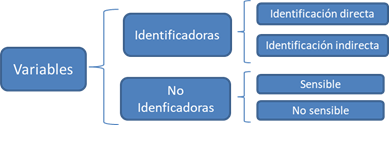
\includegraphics[width=0.6\linewidth]{Imagenes/clasi_vars} 

}

\caption{Clasificación de las variables.}\label{fig:clasVars}
\end{figure}

\hypertarget{escenarios-de-divulgaciuxf3n}{%
\section{Escenarios de divulgación}\label{escenarios-de-divulgaciuxf3n}}

La evaluación del riesgo de divulgación se lleva a cabo con referencia a las fuentes de datos disponibles en el entorno donde se liberará el conjunto de datos. En este contexto, el riesgo de divulgación es la posibilidad de volver a identificar correctamente a una unidad en el archivo de microdatos publicado \footnote{No todos los datos externos son necesariamente de dominio público. También se deben tener en cuenta los conjuntos de datos de propiedad privada o los conjuntos de datos que no se divulgan para determinar el escenario de divulgación adecuado.} comparando sus datos con un archivo externo basado en un conjunto de identificadores indirectos. La evaluación de riesgos se realiza mediante la identificación de los llamados escenarios de divulgación o intrusión. Un escenario de divulgación describe la información potencialmente disponible para el intruso (por ejemplo, datos del censo, padrones electorales, registros de población o datos recopilados por empresas privadas) para identificar a los informantes y las formas en que dicha información puede combinarse con el conjunto de microdatos que se liberará y utilizará para reidentificación de registros en el conjunto de datos. Normalmente, estos conjuntos de datos externos incluyen identificadores directos. En ese caso, la reidentificación de los registros en el conjunto de datos publicado conduce a la divulgación de la identidad y, posiblemente, de los atributos. El principal resultado de la evaluación de los escenarios de divulgación es la identificación de un conjunto de identificadores indirectos (es decir, variables clave) que deben tratarse durante el proceso SDC (ver \citet{elliot2010}).

Un ejemplo de un escenario de divulgación podría ser el reconocimiento espontáneo de un informante por parte de un investigador. Por ejemplo, mientras revisa los datos, el investigador reconoce a una persona con una combinación inusual de las variables edad y estado civil. Por supuesto, esto solo puede suceder si la persona es bien conocida o es conocida por el investigador. Otro ejemplo de un escenario de divulgación para un archivo disponible públicamente sería si las variables en los datos pudieran vincularse a un registro electoral disponible públicamente. Un intruso podría hacer coincidir todo el conjunto de datos con las personas del registro. Sin embargo, esto puede ser difícil y requerir experiencia especializada, o \emph{software}, y se deben cumplir otras condiciones. Los ejemplos son que el momento en el que se recopilaron los conjuntos de datos debe coincidir aproximadamente y el contenido de las variables debe ser (casi) idéntico. Si no se cumplen estas condiciones, la coincidencia exacta es mucho menos probable.

La evaluación del riesgo de divulgación se basa en los identificadores indirectos, que se identifican en el análisis de escenarios de riesgo de divulgación. El riesgo de divulgación depende directamente de la inclusión o exclusión de variables en el conjunto de identificadores indirectos elegidos. Por lo tanto, este paso en el proceso SDC (hacer la elección de los identificadores indirectos) debe abordarse con gran reflexión y cuidado. Veremos más adelante, cuando discutamos los pasos en el proceso de SDC con más detalle, que el primer paso para cualquier oficina de estadística es realizar un ejercicio en el que se compila un inventario de todos los conjuntos de datos disponibles en el país. Se consideran tanto los conjuntos de datos publicados por la oficina nacional de estadística (como el INE) como por otras fuentes y se analiza su disponibilidad para los intrusos, así como las variables incluidas en estos conjuntos de datos.

\hypertarget{niveles-de-riesgo}{%
\section{Niveles de riesgo}\label{niveles-de-riesgo}}

Con microdatos de encuestas y censos, a menudo tenemos que preocuparnos por la divulgación a nivel individual o de unidad, es decir, identificar a los informantes individuales. Los informantes individuales suelen ser personas físicas, pero también pueden ser unidades, como empresas, escuelas, centros de salud, etc. Los archivos de microdatos suelen tener una estructura jerárquica en la que las unidades individuales pertenecen a grupos, por ejemplo, las personas pertenecen a hogares. La estructura jerárquica más común en los microdatos es la estructura del hogar en los datos de las encuestas de hogares. Por lo tanto, en esta guía, a veces llamamos al riesgo de divulgación de datos con una estructura jerárquica ``riesgo hogar''. Sin embargo, los conceptos se aplican por igual a los datos del establecimiento y otros datos con estructuras jerárquicas, como los datos de la escuela con los alumnos y profesores o los datos de la empresa con los empleados.

Veremos que es importante tener en cuenta esta estructura jerárquica al medir el riesgo de divulgación. Para los datos jerárquicos, la información recopilada en el nivel jerárquico superior (por ejemplo, nivel del hogar) sería la misma para todos los individuos del grupo que pertenecen a ese nivel jerárquico superior (por ejemplo, el hogar) {[}Los supuestos para esta medida de riesgo son estrictos y el riesgo se estima en muchos casos mayor que el riesgo real. Entre otras suposiciones, se supone que todos los individuos de la muestra también están incluidos en el archivo externo utilizado por el intruso para compararlos. Si no es así, el riesgo es mucho menor; si el individuo en el archivo liberado no está incluido en el archivo externo, la probabilidad de una coincidencia correcta es cero. Otras suposiciones son que los archivos no contienen errores y que ambos conjuntos de datos se recopilaron simultáneamente, es decir, contienen la misma información. Estos supuestos a menudo no se cumplen en general, pero son necesarios para el cálculo de una medida. Un ejemplo de una violación de las últimas suposiciones podría ocurrir si los conjuntos de datos se recopilan en diferentes puntos en el tiempo y los registros han cambiado. Esto podría suceder cuando las personas se mudan o cambian de trabajo y hace imposible la coincidencia correcta. \textbf{Los supuestos son conservadores y asumen el mayor riesgo de divulgación}.{]}. Algunos ejemplos típicos de variables que tendrían los mismos valores para todos los miembros de una misma unidad jerárquica superior son, en el caso de los hogares, las relativas a la vivienda y los ingresos del hogar. Estas variables difieren de una encuesta a otra y de un país a otro \footnote{Consulte la sección \protect\hyperlink{objetos-de-la-clase-sdcmicroobj}{Objetos de la clase \texttt{sdcMicroObj}} para obtener más información sobre los \emph{slots} y la estructura del objeto \texttt{sdcMicro}.}. Esta estructura jerárquica crea un mayor nivel de riesgo de divulgación por dos razones:

\begin{enumerate}
\def\labelenumi{\arabic{enumi}.}
\item
  si se reidentifica a una persona del hogar, la estructura del hogar permite la reidentificación de los demás miembros del hogar en el mismo hogar,
\item
  los valores de las variables para otros miembros del hogar que son comunes para todos los miembros del hogar pueden usarse para volver a identificar a otro individuo del mismo hogar. Esto se analiza con más detalle en la sección \protect\hyperlink{riesgo-jeruxe1rquico-o-del-hogar}{Riesgo jerárquico (o del hogar)}.
\end{enumerate}

A continuación, primero analizamos las medidas de riesgo utilizadas para evaluar el riesgo de divulgación en ausencia de una estructura jerárquica. Esto incluye medidas de riesgo que buscan agregar el riesgo individual para todos los individuos en el archivo de microdatos; el objetivo es cuantificar una medida de riesgo de divulgación global para el archivo. Luego discutimos cómo cambian las medidas de riesgo cuando se tiene en cuenta la estructura jerárquica de los datos.

También discutiremos cómo las medidas de riesgo difieren para los identificadores indirectos categóricos y continuos. Para las variables categóricas, utilizaremos el concepto de unicidad de combinaciones de valores de identificadores indirectos (las llamadas ``claves'') que se utilizan para identificar a las personas en riesgo. El concepto de unicidad, sin embargo, no es útil para variables continuas, ya que es probable que todos o muchos individuos tengan valores únicos para esa variable, por definición de una variable continua. Las medidas de riesgo para variables categóricas son generalmente medidas a priori, es decir, pueden evaluarse antes de aplicar métodos de anonimización ya que se basan en el principio de unicidad. Las medidas de riesgo para variables continuas son medidas a posteriori; se basan en la comparación de los microdatos antes y después de la anonimización y son, por ejemplo, basadas en la proximidad de observaciones entre conjuntos de datos originales y tratados (anonimizados).

Los archivos que se limitan solo a identificadores indirectos categóricos o continuos son los más fáciles para medir el riesgo. Veremos en secciones posteriores que, en los casos en que ambos tipos de variables están presentes, la recodificación de variables continuas en categorías es un enfoque para simplificar el proceso SDC, pero también veremos que desde una perspectiva de utilidad esto puede no ser deseable. Un ejemplo podría ser el uso de quintiles de ingresos en lugar de las variables de ingresos reales. Veremos que medir el riesgo de divulgación con base en las variables categóricas y continuas por separado generalmente no es un enfoque válido.

Las medidas de riesgo discutidas en la siguiente sección se basan en varios supuestos. En general, estas medidas se basan en suposiciones bastante restrictivas y, a menudo, conducirán a estimaciones de riesgo conservadoras. Estas medidas de riesgo conservadoras pueden exagerar el riesgo ya que suponen el peor de los casos. Sin embargo, se deben cumplir dos suposiciones para que las medidas de riesgo sean válidas y significativas; los microdatos deben ser una muestra de una población más grande (no censo) y las ponderaciones de la muestra deben estar disponibles.

\hypertarget{riesgo-individual}{%
\section{Riesgo individual}\label{riesgo-individual}}

\hypertarget{identificadores-indirectos-categuxf3ricos-y-recuentos-de-frecuencia}{%
\subsection{Identificadores indirectos categóricos y recuentos de frecuencia}\label{identificadores-indirectos-categuxf3ricos-y-recuentos-de-frecuencia}}

El enfoque principal de la medición del riesgo para los identificadores indirectos categóricos es la divulgación de la identidad. La medición del riesgo de divulgación se basa en la evaluación de la probabilidad de reidentificación correcta de las personas en los datos publicados. Utilizamos medidas basadas en los microdatos reales que se publicarán. En general, cuanto más rara sea la combinación de valores de los identificadores indirectos (es decir, clave) de una observación en la muestra, mayor será el riesgo de revelación de identidad. Un intruso que intente hacer coincidir a una persona que tiene una clave relativamente rara dentro de los datos de muestra con un conjunto de datos externo en el que existe la misma clave tendrá una mayor probabilidad de encontrar una coincidencia correcta que cuando un número mayor de personas comparten la misma clave. Esto se puede ilustrar con el siguiente ejemplo que se ilustra en la Tabla \ref{tab:tabMR1}.

La Tabla \ref{tab:tabMR1} muestra los valores de 10 informantes para los identificadores indirectos ``área'', ``género'', ``nivel educacional'' y ``situación laboral''. En los datos, encontramos siete combinaciones únicas de valores de identificadores indirectos (es decir, patrones o claves) de los cuatro identificadores indirectos. Ejemplos de claves son \{`urbano', `femenino', `secundaria incompleta', `ocupado'\} y \{`urbano', `femenino', `primaria incompleta', `no FL'\}. Sea \(f_{k}\) la frecuencia de muestreo de la \emph{k-ésima} clave, es decir, el número de individuos de la muestra con valores de los identificadores indirectos que coinciden con la clave \emph{k}. Este sería 2 para la clave \{urbano, femenino, secundaria incompleta, ocupado\}, ya que esta clave es compartida por los individuos 1 y 2 y 1 para la clave \{`urbano', `femenino', `primaria incompleta', `no FL'\}, que es exclusivo del individuo 3. Por definición, \(f_{k}\) es el mismo para cada registro que comparte una clave particular.

\begin{table}

\caption{\label{tab:tabMR1}Conjunto de datos de ejemplo que muestra frecuencias de muestra, frecuencias de población y riesgo de divulgación individual}
\centering
\begin{tabular}[t]{c|c|c|c|c|c|c|c|c}
\hline
Id & Área & Género & Nivel educacional & Situación laboral & Peso (\$w\_\{i\}\$) & \$f\_\{k\}\$ & \$F\_\{k\}\$  & Riesgo (\$r\_\{k\}\$)\\
\hline
1 & Urbano & Femenino & Secundaria incompleta & Ocupado & 180 & 2 & 360 & 0.0054\\
\hline
2 & Urbano & Femenino & Secundaria incompleta & Ocupado & 180 & 2 & 360 & 0.0054\\
\hline
3 & Urbano & Femenino & Primaria incompleta & No FL & 215 & 1 & 215 & 0.0251\\
\hline
4 & Urbano & Masculino & Secundaria completa & Ocupado & 76 & 2 & 152 & 0.0126\\
\hline
5 & Rural & Femenino & Secundaria completa & Desocupado & 186 & 1 & 186 & 0.0282\\
\hline
6 & Urbano & Masculino & Secundaria completa & Ocupado & 76 & 2 & 152 & 0.0126\\
\hline
7 & Urbano & Femenino & Primaria completa & No FL & 180 & 1 & 180 & 0.029\\
\hline
8 & Urbano & Masculino & Post secundaria & Desocupado & 215 & 1 & 215 & 0.0251\\
\hline
9 & Urbano & Femenino & Secundaria incompleta & No FL & 186 & 2 & 262 & 0.0074\\
\hline
10 & Urbano & Femenino & Secundaria incompleta & No FL & 76 & 2 & 262 & 0.0074\\
\hline
\end{tabular}
\end{table}

Fuente: Adaptación de \citep[p.28]{benschop}

Cuanto menos personas con las que una persona comparte su combinación de identificadores indirectos, más probable es que la persona coincida correctamente en otro conjunto de datos que contenga estos identificadores indirectos. Incluso cuando los identificadores directos se eliminan del conjunto de datos, esa persona tiene un mayor riesgo de divulgación que otras, suponiendo que sus pesos de muestra sean los mismos. La Tabla \ref{tab:tabMR1} reporta las frecuencias de muestreo \(f_{k}\) de las llaves para todos los individuos. Las personas con las mismas claves tienen la misma frecuencia de muestreo. Si \(f_{k}=1\), este individuo tiene una combinación única de valores de identificadores indirectos y se denomina ``muestra única''. El conjunto de datos de la Tabla \ref{tab:tabMR1} contiene cuatro muestras únicas. Las medidas de riesgo se basan en esta frecuencia de muestreo.

En el Bloque \ref{exm:bloqueMR1}, mostramos cómo usar el paquete \texttt{sdcMicro} para crear una lista de frecuencias de muestra \(f_{k}\) para cada registro en un conjunto de datos. Esto se hace usando la función \texttt{sdcMicro} \texttt{freq()}. Un valor de 2 para una observación significa que en la muestra hay un individuo más con exactamente la misma combinación de valores para los identificadores indirectos seleccionados. En el Bloque \ref{exm:bloqueMR1}, la función \texttt{freq()} se aplica a ``sdcInitial'', que es un objeto \texttt{sdcMicro}. Los objetos se usan cuando se hace SDC con \texttt{sdcMicro}. La función \texttt{freq()} muestra la frecuencia de muestreo de las claves construidas sobre un conjunto definido de identificadores indirectos. El Bloque \ref{exm:bloqueMR1} corresponde a los datos de la Tabla \ref{tab:tabMR1}.

\begin{example}
\protect\hypertarget{exm:bloqueMR1}{}\label{exm:bloqueMR1}Cálculo \(f_{k}\) usando \texttt{sdcMicro}
\end{example}

\begin{Shaded}
\begin{Highlighting}[]
\FunctionTok{setwd}\NormalTok{(}\StringTok{"..\textbackslash{}Capacitación\textbackslash{}GitHub"}\NormalTok{) }\CommentTok{\# directorio de trabajo}

\FunctionTok{library}\NormalTok{(sdcMicro) }\CommentTok{\# carga paquete sdcMicro}
\CommentTok{\# Set up conjunto de datos}
\NormalTok{data }\OtherTok{\textless{}{-}} \FunctionTok{as.data.frame}\NormalTok{(}\FunctionTok{cbind}\NormalTok{(}\FunctionTok{as.factor}\NormalTok{(}\FunctionTok{c}\NormalTok{(}\StringTok{\textquotesingle{}Urbano\textquotesingle{}}\NormalTok{, }\StringTok{\textquotesingle{}Urbano\textquotesingle{}}\NormalTok{, }\StringTok{\textquotesingle{}Urbano\textquotesingle{}}\NormalTok{, }\StringTok{\textquotesingle{}Urbano\textquotesingle{}}\NormalTok{,}
                                        \StringTok{\textquotesingle{}Rural\textquotesingle{}}\NormalTok{, }\StringTok{\textquotesingle{}Urbano\textquotesingle{}}\NormalTok{, }\StringTok{\textquotesingle{}Urbano\textquotesingle{}}\NormalTok{, }\StringTok{\textquotesingle{}Urbano\textquotesingle{}}\NormalTok{,}
                                        \StringTok{\textquotesingle{}Urbano\textquotesingle{}}\NormalTok{, }\StringTok{\textquotesingle{}Urbano\textquotesingle{}}\NormalTok{)),}
                            \FunctionTok{as.factor}\NormalTok{(}\FunctionTok{c}\NormalTok{(}\StringTok{\textquotesingle{}Femenino\textquotesingle{}}\NormalTok{, }\StringTok{\textquotesingle{}Femenino\textquotesingle{}}\NormalTok{, }\StringTok{\textquotesingle{}Femenino\textquotesingle{}}\NormalTok{,}
                                        \StringTok{\textquotesingle{}Masculino\textquotesingle{}}\NormalTok{,}\StringTok{\textquotesingle{}Femenino\textquotesingle{}}\NormalTok{, }\StringTok{\textquotesingle{}Masculino\textquotesingle{}}\NormalTok{,}
                                        \StringTok{\textquotesingle{}Femenino\textquotesingle{}}\NormalTok{, }\StringTok{\textquotesingle{}Masculino\textquotesingle{}}\NormalTok{, }\StringTok{\textquotesingle{}Femenino\textquotesingle{}}\NormalTok{,}
                                        \StringTok{\textquotesingle{}Femenino\textquotesingle{}}\NormalTok{)),}
                            \FunctionTok{as.factor}\NormalTok{(}\FunctionTok{c}\NormalTok{(}\StringTok{\textquotesingle{}Sec in\textquotesingle{}}\NormalTok{, }\StringTok{\textquotesingle{}Sec in\textquotesingle{}}\NormalTok{, }\StringTok{\textquotesingle{}Prim in\textquotesingle{}}\NormalTok{, }\StringTok{\textquotesingle{}Sec com\textquotesingle{}}\NormalTok{,}
                                        \StringTok{\textquotesingle{}Sec com\textquotesingle{}}\NormalTok{, }\StringTok{\textquotesingle{}Sec com\textquotesingle{}}\NormalTok{, }\StringTok{\textquotesingle{}Prim com\textquotesingle{}}\NormalTok{, }\StringTok{\textquotesingle{}Post{-}sec\textquotesingle{}}\NormalTok{,}
                                        \StringTok{\textquotesingle{}Sec in\textquotesingle{}}\NormalTok{, }\StringTok{\textquotesingle{}Sec in\textquotesingle{}}\NormalTok{)),}
                            \FunctionTok{as.factor}\NormalTok{(}\FunctionTok{c}\NormalTok{(}\StringTok{\textquotesingle{}Ocu\textquotesingle{}}\NormalTok{, }\StringTok{\textquotesingle{}Ocu\textquotesingle{}}\NormalTok{, }\StringTok{\textquotesingle{}No{-}FL\textquotesingle{}}\NormalTok{, }\StringTok{\textquotesingle{}Ocu\textquotesingle{}}\NormalTok{, }\StringTok{\textquotesingle{}Desocu\textquotesingle{}}\NormalTok{, }\StringTok{\textquotesingle{}Ocu\textquotesingle{}}\NormalTok{,}
                                        \StringTok{\textquotesingle{}No{-}FL\textquotesingle{}}\NormalTok{, }\StringTok{\textquotesingle{}Desocu\textquotesingle{}}\NormalTok{, }\StringTok{\textquotesingle{}No{-}FL\textquotesingle{}}\NormalTok{,}\StringTok{\textquotesingle{}No{-}FL\textquotesingle{}}\NormalTok{)),}
                            \FunctionTok{as.factor}\NormalTok{(}\FunctionTok{c}\NormalTok{(}\StringTok{\textquotesingle{}Sí\textquotesingle{}}\NormalTok{, }\StringTok{\textquotesingle{}Sí\textquotesingle{}}\NormalTok{, }\StringTok{\textquotesingle{}Sí\textquotesingle{}}\NormalTok{, }\StringTok{\textquotesingle{}Sí\textquotesingle{}}\NormalTok{, }\StringTok{\textquotesingle{}Sí\textquotesingle{}}\NormalTok{, }\StringTok{\textquotesingle{}No\textquotesingle{}}\NormalTok{, }\StringTok{\textquotesingle{}No\textquotesingle{}}\NormalTok{,}
                                        \StringTok{\textquotesingle{}Sí\textquotesingle{}}\NormalTok{, }\StringTok{\textquotesingle{}No\textquotesingle{}}\NormalTok{, }\StringTok{\textquotesingle{}Sí\textquotesingle{}}\NormalTok{)),}
                            \FunctionTok{c}\NormalTok{(}\DecValTok{180}\NormalTok{, }\DecValTok{180}\NormalTok{, }\DecValTok{215}\NormalTok{, }\DecValTok{76}\NormalTok{, }\DecValTok{186}\NormalTok{, }\DecValTok{76}\NormalTok{, }\DecValTok{180}\NormalTok{, }\DecValTok{215}\NormalTok{, }\DecValTok{186}\NormalTok{, }\DecValTok{76}\NormalTok{)}
\NormalTok{))}

\CommentTok{\# Especificar nombres de variables}
\FunctionTok{names}\NormalTok{(data) }\OtherTok{\textless{}{-}} \FunctionTok{c}\NormalTok{(}\StringTok{\textquotesingle{}Área\textquotesingle{}}\NormalTok{, }\StringTok{\textquotesingle{}Género\textquotesingle{}}\NormalTok{, }\StringTok{\textquotesingle{}Educ\textquotesingle{}}\NormalTok{, }\StringTok{\textquotesingle{}SitLab\textquotesingle{}}\NormalTok{, }\StringTok{\textquotesingle{}Salud\textquotesingle{}}\NormalTok{, }\StringTok{\textquotesingle{}Pesos\textquotesingle{}}\NormalTok{)               }

\CommentTok{\# Set up objeto sdcMicro con especificación de identificadores indirectos y pesos}
\NormalTok{sdcInitial }\OtherTok{\textless{}{-}} \FunctionTok{createSdcObj}\NormalTok{(}\AttributeTok{dat =}\NormalTok{ data, }\AttributeTok{keyVars =} \FunctionTok{c}\NormalTok{(}\StringTok{\textquotesingle{}Área\textquotesingle{}}\NormalTok{, }\StringTok{\textquotesingle{}Género\textquotesingle{}}\NormalTok{, }\StringTok{\textquotesingle{}Educ\textquotesingle{}}\NormalTok{, }\StringTok{\textquotesingle{}SitLab\textquotesingle{}}\NormalTok{),}
                           \AttributeTok{weightVar =} \StringTok{\textquotesingle{}Pesos\textquotesingle{}}\NormalTok{)}
\NormalTok{data}\SpecialCharTok{$}\NormalTok{fk}\OtherTok{\textless{}{-}}\FunctionTok{freq}\NormalTok{(sdcInitial, }\AttributeTok{type =} \StringTok{\textquotesingle{}fk\textquotesingle{}}\NormalTok{)}
\end{Highlighting}
\end{Shaded}

Para datos de muestra, es más interesante mirar \(F_{k}\), la frecuencia de población de una combinación de identificadores indirectos (clave) \emph{k}, que es el número de individuos de la población con la clave que corresponde a la clave \emph{k}. Se desconoce la frecuencia poblacional si los microdatos son una muestra y no un censo. Bajo ciertas suposiciones, el valor esperado de las frecuencias de la población se puede calcular utilizando el peso del diseño de la muestra \(w_{i}\)(en una muestra simple, esta es la inversa de la probabilidad de inclusión) para cada individuo \emph{i}.

\[F_{k}=\sum_{i|individuo\,i\, correspondiente\, a\, la\, clave\, k} w_{i}\]

\(F_{k}\) es la suma de los pesos muestrales de todos los registros con la misma clave \emph{k}. Por lo tanto, como \(f_{k}\), \(F_{k}\) es el mismo para cada registro con clave \emph{k}. El riesgo de una reidentificación correcta es la probabilidad de que la clave coincida con el individuo correcto de la población. Dado que cada individuo en la muestra con clave \emph{k} corresponde a \(F_{k}\) individuos en la población, la probabilidad de reidentificación correcta es \(1/F_{k}\). Esta es la probabilidad de reidentificación en el peor de los casos y puede interpretarse como riesgo de divulgación. Los individuos con la misma clave tienen las mismas frecuencias, es decir, la frecuencia de la clave.

Si \(F_{k}=1\), la clave \emph{k} es tanto una muestra como una población única y el riesgo de divulgación sería 1. Las características únicas de la población son un factor importante a considerar al evaluar el riesgo y merecen especial atención.

Además, \(f_{k}\), la frecuencia de muestreo de la clave \emph{k} (es decir, el número de individuos en la muestra con la combinación de identificadores indirectos correspondientes a la combinación especificada en la clave \emph{k}) y \(F_{k}\), la frecuencia de población estimada de \emph{k}, se puede visualizar en \texttt{sdcMicro}. El Bloque \ref{exm:bloqueMR2} ilustra cómo devolver listas de longitud \emph{n} de frecuencias para todos los individuos. Las frecuencias se muestran para cada individuo y no para cada clave.

\begin{example}
\protect\hypertarget{exm:bloqueMR2}{}\label{exm:bloqueMR2}Cálculo de frecuencias muestrales y poblacionales usando \texttt{sdcMicro}
\end{example}

\begin{Shaded}
\begin{Highlighting}[]
\CommentTok{\# frecuencia muestral de individuos}
\NormalTok{data}\SpecialCharTok{$}\NormalTok{fk}\OtherTok{\textless{}{-}}\FunctionTok{freq}\NormalTok{(sdcInitial, }\AttributeTok{type =} \StringTok{\textquotesingle{}fk\textquotesingle{}}\NormalTok{)}
\CommentTok{\# frecuencia poblacional de individuos}
\NormalTok{data}\SpecialCharTok{$}\NormalTok{FK}\OtherTok{\textless{}{-}}\FunctionTok{freq}\NormalTok{(sdcInitial, }\AttributeTok{type =} \StringTok{\textquotesingle{}Fk\textquotesingle{}}\NormalTok{)}
\end{Highlighting}
\end{Shaded}

En la práctica, este enfoque conduce a estimaciones de riesgo conservadoras, ya que no tiene en cuenta adecuadamente los métodos de muestreo. En este caso, las estimaciones del riesgo de reidentificación pueden ser demasiado altas. Si se utiliza este riesgo sobreestimado, los datos pueden estar sobreprotegidos (es decir, la pérdida de información será mayor que la necesaria) al aplicar las medidas de SDC.

La medida del riesgo \(r_{k}\) es como \(f_{k}\) y \(F_{k}\), el mismo para todos los individuos que comparten el mismo patrón de valores de identificadores indirectos y se denomina riesgo individual. Los valores \(r_{k}\) también puede interpretarse como la probabilidad de divulgación de los individuos o como la probabilidad de una coincidencia exitosa con individuos elegidos al azar de un archivo de datos externo con los mismos valores de los identificadores indirectos. Esta medida de riesgo se basa en ciertos supuestos \footnote{Los supuestos para esta medida de riesgo son estrictos y el riesgo se estima en muchos casos mayor que el riesgo real. Entre otras suposiciones, se supone que todos los individuos de la muestra también están incluidos en el archivo externo utilizado por el intruso para compararlos. Si no es así, el riesgo es mucho menor; si el individuo en el archivo liberado no está incluido en el archivo externo, la probabilidad de una coincidencia correcta es cero. Otras suposiciones son que los archivos no contienen errores y que ambos conjuntos de datos se recopilaron simultáneamente, es decir, contienen la misma información. Estos supuestos a menudo no se cumplen en general, pero son necesarios para el cálculo de una medida. Un ejemplo de una violación de las últimas suposiciones podría ocurrir si los conjuntos de datos se recopilan en diferentes puntos en el tiempo y los registros han cambiado. Esto podría suceder cuando las personas se mudan o cambian de trabajo y hace imposible la coincidencia correcta. \textbf{Los supuestos son conservadores y asumen el mayor riesgo de divulgación}.}, que son estrictos y pueden conducir a una medida de riesgo relativamente conservadora. En \texttt{sdcMicro}, la medida de riesgo \(r_{k}\) se calcula automáticamente al crear un objeto \texttt{sdcMicro} y se guarda en el \emph{slot} de ``riesgo'' \footnote{Consulte la sección \protect\hyperlink{objetos-de-la-clase-sdcmicroobj}{Objetos de la clase \texttt{sdcMicroObj}} para obtener más información sobre los \emph{slots} y la estructura del objeto \texttt{sdcMicro}.}. El Bloque \ref{exm:bloqueMR3} muestra cómo recuperar las medidas de riesgo usando \texttt{sdcMicro} para nuestro ejemplo. Las medidas de riesgo también se presentan en la Tabla \ref{tab:tabMR1}.

\begin{example}
\protect\hypertarget{exm:bloqueMR3}{}\label{exm:bloqueMR3}Slot de riesgo individual en el objeto \texttt{sdcMicro}
\end{example}

\begin{Shaded}
\begin{Highlighting}[]
\NormalTok{sdcInitial}\SpecialCharTok{@}\NormalTok{risk}\SpecialCharTok{$}\NormalTok{individual}
\end{Highlighting}
\end{Shaded}

Los principales factores que influyen en el riesgo individual son las frecuencias de muestreo \(f_{k}\) y los pesos de diseño de muestreo \(w_{i}\). Si un individuo tiene un riesgo relativamente alto de divulgación, en nuestro ejemplo serían los individuos 3, 5, 7 y 8 en la Tabla \ref{tab:tabMR1} y el Bloque \ref{exm:bloqueMR3}, la probabilidad de que un posible intruso relacione correctamente a estos individuos con un archivo de datos externo es relativamente alta. En nuestro ejemplo, la razón del alto riesgo es el hecho de que estos individuos son muestras únicas (es decir, \(f_{k}=1\)). Este riesgo es el riesgo del peor de los casos y no implica que la persona sea reidentificada con certeza con esta probabilidad. Por ejemplo, si un individuo incluido en los microdatos no está incluido en el archivo de datos externo, la probabilidad de una coincidencia correcta es cero. No obstante, la medida del riesgo calculada a partir de las frecuencias será positiva como medida de evaluación.

\hypertarget{k-anonimato}{%
\subsection{k-anonimato}\label{k-anonimato}}

La medida del riesgo k- anonimato se basa en el principio de que, en un conjunto de datos seguro, el número de personas que comparten la misma combinación de valores (claves) de identificadores indirectos categóricos debe ser superior a un umbral especificado \emph{k}. El k-anonimato es una medida de riesgo basada en los microdatos a publicar, ya que solo tiene en cuenta la muestra. Un individuo viola el k-anonimato si la frecuencia de muestreo \(f_{k}\) para la llave \emph{k} es menor que el umbral especificado \emph{k}. Por ejemplo, si un individuo tiene la misma combinación de identificadores indirectos que otros dos individuos en la muestra, estos individuos satisfacen el 3-anonimato pero violan el 4-anonimato. En el conjunto de datos de la Tabla \ref{tab:tabMR1}, seis personas satisfacen el 2-anonimato y cuatro violan el 2-anonimato. Los individuos que violan el 2-anonimato son muestras únicas. La medida de riesgo es el número de observaciones que violan el k-anonimato para un cierto valor de \emph{k}, que es

\[ \sum_{i} I(f_{k}<k), \]

donde \(I\) es la función indicadora e \(i\) se refiere al \emph{i-ésimo} registro. Esto es simplemente un recuento del número de personas con una frecuencia de muestreo de su clave inferior a \emph{k}. El recuento es mayor para los \emph{k} más grandes, ya que si un registro satisface k-anonimato, también satisface (k+1)- anonimato. La medida del riesgo k-anonimato no considera los pesos de la muestra, pero es importante considerar los pesos de la muestra al determinar el nivel requerido de k-anonimato. Si los pesos de la muestra son grandes, un individuo en el conjunto de datos representa a más individuos en la población objetivo, la probabilidad de una coincidencia correcta es menor y, por lo tanto, el umbral requerido puede ser más bajo. Los pesos de muestra grandes van de la mano con conjuntos de datos más pequeños. En un conjunto de datos más pequeño, la probabilidad de encontrar otro registro con la misma clave es menor que en un conjunto de datos más grande. Esta probabilidad está relacionada con el número de registros en la población con una clave particular a través de los pesos muestrales.

En \texttt{sdcMicro} podemos mostrar el número de observaciones que violan un determinado umbral de k-anonimato. En el Bloque \ref{exm:bloqueMR4}, usamos \texttt{sdcMicro} para calcular la cantidad de infractores para los umbrales \(k=2\) y \(k=3\). Se da tanto el número absoluto de infractores como el número relativo como porcentaje del número de individuos en la muestra. En el ejemplo, cuatro observaciones violan el 2-anonimato y las 10 observaciones violan el 3-anonimato.

\begin{example}
\protect\hypertarget{exm:bloqueMR4}{}\label{exm:bloqueMR4}Uso de la función \texttt{print()} para mostrar observaciones que violan k-anonimato
\end{example}

\begin{Shaded}
\begin{Highlighting}[]
\FunctionTok{print}\NormalTok{(sdcInitial, }\StringTok{\textquotesingle{}kAnon\textquotesingle{}}\NormalTok{)}
\end{Highlighting}
\end{Shaded}

Para otros niveles de k-anonimato, es posible calcular el número de personas infractoras utilizando los recuentos de frecuencia de muestreo en el objeto \texttt{sdcMicro}. El número de infractores es el número de personas con recuentos de frecuencia de muestreo inferiores al umbral especificado \emph{k}. En el Bloque \ref{exm:bloqueMR5}, mostramos un ejemplo de cómo calcular cualquier umbral para \emph{k} usando las medidas de riesgo ya almacenadas disponibles después de configurar un objeto \texttt{sdcMicro} en \texttt{R}. \emph{k} se puede reemplazar con cualquier umbral requerido. La elección del umbral requerido que deben cumplir todas las personas en el archivo de microdatos depende de muchos factores y se analiza más adelante en la sección \protect\hyperlink{sup-loc}{Supresión local} sobre la supresión local. En muchas instituciones, los umbrales típicamente requeridos para k-anonimato son 3 y 5.

\begin{example}
\protect\hypertarget{exm:bloqueMR5}{}\label{exm:bloqueMR5}Violaciones de k-anonimato para distintos valores de k
\end{example}

\begin{Shaded}
\begin{Highlighting}[]
\NormalTok{k}\OtherTok{=}\DecValTok{10}
\FunctionTok{sum}\NormalTok{(sdcInitial}\SpecialCharTok{@}\NormalTok{risk}\SpecialCharTok{$}\NormalTok{individual[,}\DecValTok{2}\NormalTok{] }\SpecialCharTok{\textless{}}\NormalTok{ k)}
\end{Highlighting}
\end{Shaded}

Es importante tener en cuenta que los valores faltantes (\texttt{NA}s en \texttt{R} \footnote{En \texttt{sdcMicro}, es importante utilizar el código de valor faltante estándar \texttt{NA} en lugar de otros códigos, como 9999 o cadenas. En la sección \protect\hyperlink{valores-faltantes}{Valores faltantes}, se analizó más detalladamente cómo establecer otros códigos de valores faltantes de \texttt{NA} en \texttt{R}. Esto es necesario para garantizar que los métodos de \texttt{sdcMicro} funcionen correctamente. Cuando los valores faltantes tienen códigos distintos de \texttt{NA}, los códigos de valores faltantes se interpretan como un nivel de factor distinto en el caso de las variables categóricas.} ) se tratan como si fueran cualquier otro valor. Dos personas con claves \{`Masculino', \texttt{NA}, `Ocupado'\} y \{`Masculino', `Secundaria completa', `Ocupado'\} comparten la misma clave y, de manera similar, \{`Masculino', \texttt{NA}, `Ocupado'\} y \{`Masculino', `Secundaria incompleta', `Ocupado'\} también comparten la misma clave. Por lo tanto, el valor que falta en la primera clave se interpreta primero como `Secundaria completa' y luego como `Secundaria incompleta'. Esto se ilustra en la Tabla \ref{tab:tabMR2}.

\begin{table}

\caption{\label{tab:tabMR2}Conjunto de datos de ejemplo para ilustrar el efecto de los valores faltantes en el k-anonimato}
\centering
\begin{tabular}[t]{c|c|c|c|c}
\hline
Id & Género & Nivel educacional & Situación laboral & \$f\_\{k\}\$\\
\hline
1 & Masculino & Secundaria completa & Ocupado & 2\\
\hline
2 & Masculino & Secundaria incompleta & Ocupado & 2\\
\hline
3 & Masculino & NA & Ocupado & 3\\
\hline
\end{tabular}
\end{table}

Fuente: Adaptación de \citep[p.32]{benschop}

Si un conjunto de datos satisface k-anonimato, un intruso siempre encontrará al menos \emph{k} individuos con la misma combinación de identificadores indirectos. El k-anonimato suele ser un requisito necesario para la anonimización de un conjunto de datos antes de su publicación, pero no es necesariamente un requisito suficiente. La medida de k-anonimato solo se basa en recuentos de frecuencia y no tiene en cuenta (las diferencias en) los pesos de las muestras. Con frecuencia el k-anonimato se logra aplicando primero la recodificación y luego la supresión local y, en algunos casos, mediante la microagregación, antes de utilizar otras medidas de riesgo y métodos de divulgación para reducir aún más el riesgo de divulgación. Estos métodos se analizan en la sección \protect\hyperlink{muxe9todos-sdc}{Métodos SDC}.

\hypertarget{l-diversity}{%
\subsection{l-diversity}\label{l-diversity}}

El k-anonimato ha sido criticado por no ser lo suficientemente restrictivo. La información confidencial puede divulgarse incluso si los datos satisfacen el k-anonimato. Esto puede ocurrir en los casos en que los datos contienen variables categóricas confidenciales (de no identificación) que tienen el mismo valor para todas las personas que comparten la misma clave. Ejemplos de tales variables sensibles son aquellas que contienen información sobre el estado de salud de un individuo. La Tabla \ref{tab:tabMR3} ilustra este problema utilizando los mismos datos que se utilizaron anteriormente, pero agregando una variable sensible, ``salud''. Los dos primeros individuos cumplen 2-anonimato para los identificadores indirectos ``área'', ``género'', ``nivel educacional'' y ``situación laboral''. Esto significa que un intruso encontrará al menos dos personas al hacer coincidir el conjunto de microdatos publicado en función de esos cuatro identificadores indirectos. Sin embargo, si el intruso sabe que alguien pertenece a la muestra y tiene la clave \{`Urbano', `Femenino', `Secundaria incompleta' y `Ocupado'\}, con certeza se revela el estado de salud (`sí'), porque para ambos las observaciones con esta clave tienen el mismo valor. Esta información se revela así sin la necesidad de coincidir exactamente con el individuo. Este no es el caso de los individuos con clave \{`Urbano', `Masculino', `Secundaria completa', `Ocupado'\}.

El concepto de l-diversity (distinto) aborda esta deficiencia del k-anonimato. Un conjunto de datos satisface l-diversity si para cada clave \emph{k} hay por lo menos \emph{l} diferentes valores para cada una de las variables sensibles. En el ejemplo, los primeros dos individuos satisfacen solo 1-diversity, los individuos 4 y 6 satisfacen 2-diversity. El nivel requerido de l-diversity depende del número de valores posibles que puede tomar la variable sensible. Si la variable sensible es una variable binaria, el nivel más alto de l-diversity que se puede conseguir es 2. Una muestra única siempre solo satisfará 1-diversity.

Para computar l-diversity para variables sensibles en \texttt{sdcMicro}, se puede usar la función \texttt{ldiversity()}. Esto se ilustra en el Bloque \ref{exm:bloqueMR6}. Como argumentos, especificamos los nombres de las variables sensibles \footnote{Alternativamente, las variables sensibles se pueden especificar al crear el objeto \texttt{sdcMicro} usando la función \texttt{createSdcObj()} en el argumento sensibleVar. Esto se explica con más detalle en la sección \protect\hyperlink{objetos-de-la-clase-sdcmicroobj}{Objetos de la clase \texttt{sdcMicroObj}}. En ese caso, no es necesario especificar el argumento ldiv\_index en la función \texttt{ldiversity()}, y las variables en el argumento sensibleVar se usarán automáticamente para calcular l-diversity.} en el archivo, así como una constante para l-diversity \footnote{Además de l-diversity distintos, hay otros métodos de l-diversity: entropía y recursivo. l-diversity distinto es el más utilizado.} y el código de valores faltantes en los datos. La salida se guarda en el \emph{slot} de ``riesgo'' del objeto \texttt{sdcMicro}. El resultado muestra el mínimo, máximo, media y cuantiles de las l-puntuaciones de diversidad para todos los individuos de la muestra. El resultado del Bloque \ref{exm:bloqueMR6} reproduce los resultados según los datos de la Tabla \ref{tab:tabMR3}.

\begin{table}

\caption{\label{tab:tabMR3}Ilustración de l-diversity}
\centering
\begin{tabular}[t]{c|c|c|c|c|c|c|c|c}
\hline
Id & Área & Género & Nivel educacional & Situación laboral & Salud & \$f\_\{k\}\$ & \$F\_\{k\}\$  & l-diversity\\
\hline
1 & Urbano & Femenino & Secundaria incompleta & Ocupado & Enfermo & 2 & 360 & 1\\
\hline
2 & Urbano & Femenino & Secundaria incompleta & Ocupado & Enfermo & 2 & 360 & 1\\
\hline
3 & Urbano & Femenino & Primaria incompleta & No FL & Enfermo & 1 & 215 & 1\\
\hline
4 & Urbano & Masculino & Secundaria completa & Ocupado & Enfermo & 2 & 152 & 2\\
\hline
5 & Rural & Femenino & Secundaria completa & Desocupado & Enfermo & 1 & 186 & 1\\
\hline
6 & Urbano & Masculino & Secundaria completa & Ocupado & Sano & 2 & 152 & 2\\
\hline
7 & Urbano & Femenino & Primaria completa & No FL & Sano & 1 & 180 & 1\\
\hline
8 & Urbano & Masculino & Post secundaria & Desocupado & Enfermo & 1 & 215 & 1\\
\hline
9 & Urbano & Femenino & Secundaria incompleta & No FL & Sano & 2 & 262 & 2\\
\hline
10 & Urbano & Femenino & Secundaria incompleta & No FL & Enfermo & 2 & 262 & 2\\
\hline
\end{tabular}
\end{table}

Fuente: Adaptación de \citep[p.33]{benschop}

\begin{example}
\protect\hypertarget{exm:bloqueMR6}{}\label{exm:bloqueMR6}Función para l-diversity en \texttt{sdcMicro}
\end{example}

\begin{Shaded}
\begin{Highlighting}[]
 \CommentTok{\# Calculando l{-}diversity}

\NormalTok{ sdcInitial }\OtherTok{\textless{}{-}} \FunctionTok{ldiversity}\NormalTok{(}\AttributeTok{obj =}\NormalTok{ sdcInitial, }\AttributeTok{ldiv\_index =} \FunctionTok{c}\NormalTok{(}\StringTok{"Salud"}\NormalTok{), }
                          \AttributeTok{l\_recurs\_c =} \DecValTok{2}\NormalTok{, }\AttributeTok{missing =} \ConstantTok{NA}\NormalTok{)}
 \CommentTok{\# Resultado para l{-}diversity}
\NormalTok{ sdcInitial}\SpecialCharTok{@}\NormalTok{risk}\SpecialCharTok{$}\NormalTok{ldiversity}
 
 \CommentTok{\# l{-}diversity score para cada registro}
\NormalTok{ sdcInitial}\SpecialCharTok{@}\NormalTok{risk}\SpecialCharTok{$}\NormalTok{ldiversity[,}\StringTok{\textquotesingle{}Salud\_Distinct\_Ldiversity\textquotesingle{}}\NormalTok{]}
\end{Highlighting}
\end{Shaded}

l-diversity es útil si los datos contienen variables sensibles categóricas que no son identificadores indirectos en sí mismos. No es posible seleccionar identificadores indirectos para calcular la l-diversity. La l-diversity debe calcularse para cada variable sensible por separado.

\hypertarget{medidas-de-riesgo-para-variables-continuas}{%
\section{Medidas de riesgo para variables continuas}\label{medidas-de-riesgo-para-variables-continuas}}

El principio de rareza o unicidad de combinaciones de identificadores indirectos (claves) no es útil para variables continuas, porque es probable que todos o muchos individuos tengan claves únicas. Por lo tanto, se explotan otros enfoques para medir el riesgo de divulgación de las variables continuas. Estos métodos se basan en la unicidad de los valores en la vecindad de los valores originales. La unicidad se define de diferentes formas: en términos absolutos (medida de intervalo) o en términos relativos (vinculación de registros). La mayoría de las medidas son medidas a posteriori: se evalúan después de anonimizar los datos sin procesar, comparar los datos tratados con los datos sin procesar y evaluar para cada individuo la distancia entre los valores en los datos sin procesar y los tratados. Esto significa que estos métodos no son útiles para identificar personas en riesgo dentro de los datos sin procesar, sino que muestra la distancia/diferencia entre el conjunto de datos antes y después de la anonimización y, por lo tanto, puede interpretarse como una evaluación del método de anonimización. Por esa razón, se asemejan a las medidas de pérdida de información discutidas en la sección \protect\hyperlink{mediciuxf3n-de-la-utilidad-y-la-puxe9rdida-de-informaciuxf3n}{Medición de la utilidad y la pérdida de información}. Finalmente, las medidas de riesgo para identificadores indirectos continuos también se basan en la detección de valores atípicos. Los valores atípicos juegan un papel importante en la reidentificación de estos registros.

\hypertarget{vinculaciuxf3n-de-registros-o-coincidencia-de-registros}{%
\subsection{Vinculación de registros (o coincidencia de registros)}\label{vinculaciuxf3n-de-registros-o-coincidencia-de-registros}}

Vinculación de registros (o Record linkage, en inglés) es un método a posteriori que evalúa el número de vínculos correctos al vincular los valores perturbados con los valores originales. El algoritmo de vinculación se basa en la distancia entre el original y los valores perturbados (es decir, vinculación de registros basada en la distancia). Los valores perturbados se emparejan con el individuo más cercano. Es importante señalar que este método no brinda información sobre el riesgo inicial, sino que es una medida para evaluar el algoritmo de perturbación (es decir, está diseñado para indicar el nivel de incertidumbre introducido en la variable al contar la cantidad de registros que podría coincidir correctamente).

Los algoritmos de vinculación de registros difieren con respecto a qué medida de distancia se utiliza. Cuando una variable tiene una escala muy diferente a la de otras variables continuas en el conjunto de datos, se recomienda volver a escalar las variables antes de usar la vinculación de registros. Escalas muy diferentes pueden dar lugar a resultados no deseados al medir la distancia multivariada entre registros en función de varias variables continuas. Dado que estos métodos se basan tanto en datos sin procesar como en datos tratados, los ejemplos de sus aplicaciones requieren la introducción de métodos SDC y, por lo tanto, se posponen a los estudios de casos en la sección \protect\hyperlink{caso-de-estudio}{Caso de estudio}.

Además de la vinculación de registros basada en la distancia, otro método de vinculación es la vinculación de registros probabilísticos. La literatura muestra, sin embargo, que los resultados de la vinculación de registros basados en la distancia son mejores que los resultados de la vinculación de registros probabilísticos. Las personas en los datos tratados que están vinculadas a las personas correctas en los datos sin procesar se consideran en riesgo de divulgación.

\hypertarget{medida-de-intervalo}{%
\subsection{Medida de intervalo}\label{medida-de-intervalo}}

La aplicación exitosa de un método SDC debería dar como resultado valores perturbados que no se consideran demasiado cercanos a sus valores iniciales; si el valor es relativamente cercano, la reidentificación puede ser relativamente fácil. En la aplicación de medidas de intervalo, se crean intervalos alrededor de cada valor perturbado y luego se determina si el valor original de esa observación perturbada está contenido en este intervalo. Los valores que están dentro del intervalo alrededor del valor inicial después de la perturbación se consideran demasiado cercanos al valor inicial y, por lo tanto, no son seguros y necesitan más perturbaciones. Los valores que están fuera de los intervalos se consideran seguros. El tamaño de los intervalos se basa en la desviación estándar de las observaciones y un parámetro de escala. Este método está implementado en la función \texttt{dRisk()} en \texttt{sdcMicro}. El Bloque \ref{exm:bloqueMR7} muestra cómo imprimir o mostrar el valor de riesgo calculado por \texttt{sdcMicro} comparando las variables de ingresos antes y después de la anonimización. ``sdcObj'' es un objeto \texttt{sdcMicro} y ``compExp`` es un vector que contiene los nombres de las variables de ingresos. El tamaño de los intervalos es \emph{k} veces la desviación estándar, donde \emph{k} es un parámetro en la función \texttt{dRisk()}. El más largo \emph{k}, cuanto más grandes son los intervalos y, por lo tanto, mayor es el número de observaciones dentro del intervalo construidas alrededor de sus valores originales y mayor es la medida de riesgo. El resultado 1 indica que todas (100 por ciento) las observaciones están fuera del intervalo de 0,1 veces la desviación estándar alrededor de los valores originales.

\begin{example}
\protect\hypertarget{exm:bloqueMR7}{}\label{exm:bloqueMR7}Ilustración de medida de intervalo
\end{example}

\begin{Shaded}
\begin{Highlighting}[]
 \FunctionTok{dRisk}\NormalTok{(}\AttributeTok{obj =}\NormalTok{ sdcObj}\SpecialCharTok{@}\NormalTok{origData[,compExp], }\AttributeTok{xm =}\NormalTok{ sdcObj}\SpecialCharTok{@}\NormalTok{manipNumVars[,compExp],}
       \AttributeTok{k =} \FloatTok{0.1}\NormalTok{)}
\NormalTok{ [}\DecValTok{1}\NormalTok{] }\DecValTok{1}
\end{Highlighting}
\end{Shaded}

Para la mayoría de los valores, este es un enfoque satisfactorio. Sin embargo, no es una medida suficiente para valores atípicos. Después de la perturbación, los valores atípicos seguirán siendo valores atípicos y se pueden volver a identificar fácilmente, incluso si están lo suficientemente lejos de sus valores iniciales. Por lo tanto, los valores atípicos deben tratarse con precaución.

\hypertarget{detecciuxf3n-de-valores-atuxedpicos}{%
\subsection{Detección de valores atípicos}\label{detecciuxf3n-de-valores-atuxedpicos}}

Los valores atípicos son importantes para medir el riesgo de reidentificación en microdatos continuos. Los datos continuos suelen estar sesgados, especialmente a la derecha. Esto significa que hay algunos valores atípicos con valores muy altos en relación con las otras observaciones de la misma variable. Algunos ejemplos son los ingresos en los datos de los hogares, donde solo unas pocas personas/hogares pueden tener ingresos muy altos, o los datos de facturación de empresas que son mucho más grandes que otras empresas de la muestra. En casos como estos, incluso si estos valores se perturban, aún puede ser fácil identificar estos valores atípicos, ya que seguirán siendo los valores más grandes incluso después de la perturbación (la perturbación habrá creado incertidumbre en cuanto al valor exacto, pero debido a que el valor comenzó mucho más lejos de otras observaciones, aún puede ser fácil vincularlo con el individuo de altos ingresos o la empresa muy grande). Los ejemplos serían el único médico en un área geográfica con altos ingresos o una sola gran empresa en un tipo de industria. Por lo tanto, la identificación de valores atípicos en datos continuos es un paso importante cuando se identifican personas con alto riesgo. En la práctica, identificar los valores de una variable continua que son mayores que un valor predeterminado p\%-percentil podría ayudar a identificar valores atípicos y, por lo tanto, unidades con mayor riesgo de identificación. El valor de \emph{p} depende de la asimetría de los datos.

Podemos calcular el p\%-percentil de una variable continua en \texttt{R} y mostrar los individuos que tienen ingresos superiores a este percentil. El Bloque \ref{exm:bloqueMR8} proporciona una ilustración del percentil 90.

\begin{example}
\protect\hypertarget{exm:bloqueMR8}{}\label{exm:bloqueMR8}Cómputo del percentil 90 \% de la variable INCWAGE
\end{example}

\begin{Shaded}
\begin{Highlighting}[]
\FunctionTok{setwd}\NormalTok{(}\StringTok{"../Capacitación/GitHub"}\NormalTok{) }\CommentTok{\# directorio de trabajo}

\NormalTok{fname }\OtherTok{=} \StringTok{"data.dta"} \CommentTok{\# nombre del archivo}
\FunctionTok{library}\NormalTok{(haven) }\CommentTok{\# carga el paquete requerido para la función de lectura/escritura}
               \CommentTok{\# para archivos STATA}
\NormalTok{file }\OtherTok{\textless{}{-}} \FunctionTok{read\_dta}\NormalTok{(fname) }

\CommentTok{\# Cómputo de 90 \% percentil para variable INCWAGE}
\NormalTok{ perc90 }\OtherTok{\textless{}{-}} \FunctionTok{quantile}\NormalTok{(file[,}\StringTok{\textquotesingle{}INCWAGE\textquotesingle{}}\NormalTok{], }\FloatTok{0.90}\NormalTok{, }\AttributeTok{na.rm =} \ConstantTok{TRUE}\NormalTok{)}

 \CommentTok{\# Muestra ID de observaciones con valores para INCWAGE mayores al 90 \% percentil}
\NormalTok{ file[(file[, }\StringTok{\textquotesingle{}INCWAGE\textquotesingle{}}\NormalTok{] }\SpecialCharTok{\textgreater{}=}\NormalTok{ perc90), }\StringTok{\textquotesingle{}IDP\textquotesingle{}}\NormalTok{]}
\end{Highlighting}
\end{Shaded}

Un segundo enfoque para la detección de valores atípicos es una medida a posteriori que compara los datos tratados y sin procesar. Se construye un intervalo alrededor de los valores perturbados como se describe en la sección anterior. Si los valores originales caen dentro del intervalo alrededor de los valores perturbados, los valores perturbados se consideran inseguros ya que están demasiado cerca de los valores originales. Existen diferentes formas de construir dichos intervalos, como intervalos basados en rangos e intervalos basados en desviación estándar. \citet{templ2008} proponen una alternativa robusta para estos intervalos. Construyen los intervalos en función de la distancia robusta de Mahalanobis (RMD, por su sigla en inglés) al cuadrado de los valores individuales. El RMD escala los intervalos de manera que los valores atípicos obtienen intervalos más grandes y, por lo tanto, deben tener una perturbación mayor para que se consideren seguros que los valores que no son atípicos. Este método se implementa en \texttt{sdcMicro} en la función \texttt{dRiskRMD()}, que es una extensión de la función \texttt{dRisk()}.

\hypertarget{riesgo-global}{%
\section{Riesgo global}\label{riesgo-global}}

Para construir una medida de riesgo agregado a nivel global para el conjunto de datos completo, podemos agregar las medidas de riesgo a nivel individual de varias maneras. Las medidas de riesgo global deben usarse con precaución: detrás de un riesgo global aceptable pueden esconderse algunos registros de muy alto riesgo que se compensan con muchos registros de bajo riesgo.

\hypertarget{media-de-las-medidas-de-riesgo-individuales}{%
\subsection{Media de las medidas de riesgo individuales}\label{media-de-las-medidas-de-riesgo-individuales}}

Una forma sencilla de agregar las medidas de riesgo individuales es tomar la media de todos los individuos de la muestra, que es igual a sumar todas las claves de la muestra si se multiplica por las frecuencias de muestra de estas claves y se divide por el tamaño de la muestra, \(n\):

\[R_{1}=\frac{1}{n}\sum_{i} r_{k}=\frac{1}{n}\sum_{k}f_{k}r_{k},\]

donde \(r_{k}\) es el riesgo individual de clave \(k\) que el \emph{i-ésimo} registro comparte (ver la sección \protect\hyperlink{identificadores-indirectos-categuxf3ricos-y-recuentos-de-frecuencia}{Identificadores indirectos categóricos y recuentos de frecuencia}). Esta medida se informa como riesgo global en \texttt{sdcMicro}, se almacena en el \emph{slot} de ``riesgo'' y se puede imprimir como se muestra en el Bloque \ref{exm:bloqueMR9}. Indica que la probabilidad de reidentificación promedio es 0,01582 o 0,1582\%.

\begin{example}
\protect\hypertarget{exm:bloqueMR9}{}\label{exm:bloqueMR9}Cómputo de la medida de riesgo global
\end{example}

\begin{Shaded}
\begin{Highlighting}[]
\CommentTok{\# Riesgo global (probabilidad promedio de re{-}identificación)}
\NormalTok{ sdcInitial}\SpecialCharTok{@}\NormalTok{risk}\SpecialCharTok{$}\NormalTok{global}\SpecialCharTok{$}\NormalTok{risk}
\end{Highlighting}
\end{Shaded}

El riesgo global en los datos de ejemplo de la Tabla \ref{tab:tabMR1} es 0,01582, que es la proporción esperada de todos los individuos de la muestra que un intruso podría volver a identificar. Otra forma de expresar el riesgo global es el número de reidentificaciones esperadas, \(n*R_{1}\), que es en el ejemplo 10 * 0,01582. El número esperado de reidentificaciones también se guarda en el objeto \texttt{sdcMicro}. El Bloque \ref{exm:bloqueMR10} muestra cómo imprimir esto.

\begin{example}
\protect\hypertarget{exm:bloqueMR10}{}\label{exm:bloqueMR10}Cómputo del número esperado de reidentificaciones
\end{example}

\begin{Shaded}
\begin{Highlighting}[]
\CommentTok{\#  \# Riesgo global(Número esperado de re{-}identificaciones)}
\NormalTok{ sdcInitial}\SpecialCharTok{@}\NormalTok{risk}\SpecialCharTok{$}\NormalTok{global}\SpecialCharTok{$}\NormalTok{risk\_ER}
\end{Highlighting}
\end{Shaded}

\hypertarget{recuento-de-personas-con-riesgos-superiores-a-un-cierto-umbral}{%
\subsection{Recuento de personas con riesgos superiores a un cierto umbral}\label{recuento-de-personas-con-riesgos-superiores-a-un-cierto-umbral}}

Todos los individuos pertenecientes a la misma clave tienen el mismo riesgo individual, \(r_{k}\). Otra forma de expresar el riesgo total en la muestra es el número total de observaciones que superan un determinado umbral de riesgo individual. La fijación del umbral puede ser absoluta (por ejemplo, todas aquellas personas que tengan un riesgo de divulgación superior a 0,05 o 5\%) o relativa (por ejemplo, todas aquellas personas con riesgos superiores al cuartil superior del riesgo individual). El Bloque \ref{exm:bloqueMR11} muestra cómo utilizando \texttt{R}, se contaría el número de observaciones con un riesgo de reidentificación individual superior al 5\%. En el ejemplo, ninguna persona tiene un riesgo de divulgación superior a 0,05.

\begin{example}
\protect\hypertarget{exm:bloqueMR11}{}\label{exm:bloqueMR11}Número de personas con riesgo individual superior al umbral 0,05
\end{example}

\begin{Shaded}
\begin{Highlighting}[]
 \FunctionTok{sum}\NormalTok{(sdcInitial}\SpecialCharTok{@}\NormalTok{risk}\SpecialCharTok{$}\NormalTok{individual[,}\DecValTok{1}\NormalTok{] }\SpecialCharTok{\textgreater{}} \FloatTok{0.05}\NormalTok{)}
\end{Highlighting}
\end{Shaded}

Estos cálculos se pueden usar para tratar los datos de las personas cuyos valores de riesgo están por encima de un umbral predeterminado. Más adelante veremos que hay métodos en \texttt{sdcMicro}, como \texttt{localSupp()}, que se pueden usar para suprimir valores de ciertas variables clave para aquellas personas con riesgo por encima de un umbral específico. Esto se explica con más detalle en la sección \protect\hyperlink{sup-loc}{Supresión local}.

\hypertarget{riesgo-jeruxe1rquico-o-del-hogar}{%
\section{Riesgo jerárquico (o del hogar)}\label{riesgo-jeruxe1rquico-o-del-hogar}}

En muchas encuestas sociales, los datos tienen una estructura jerárquica donde un individuo pertenece a una entidad de nivel superior (ver la sección \protect\hyperlink{niveles-de-riesgo}{Niveles de riesgo}). Ejemplos típicos son los hogares en las encuestas sociales o los alumnos en las escuelas. La reidentificación de un miembro del hogar también puede conducir a la reidentificación de los otros miembros del hogar. Por tanto, es fácil ver que, si tenemos en cuenta la estructura del hogar, el riesgo de reidentificación es el riesgo de que al menos uno de los miembros del hogar sea reidentificado.

\[r^h=P(A_{1}\bigcup A_{2}\bigcup \dots \bigcup A_{J})=1-\prod_{j=1}^J 1-P(A_{j}), \]
donde \(A_{j}\) es el evento que el \emph{j-ésimo} miembro del hogar sea identificado y \(P(A_{j})=r_{k}\) es el riesgo de divulgación individual del \emph{j-ésimo} miembro. Por ejemplo, si un hogar tiene tres miembros con riesgos de divulgación individuales en función de sus respectivas claves 0,02, 0,03 y 0,03, respectivamente, el riesgo del hogar es

\[1-((1-0,02)(1-0,03)(1-0,03))=0,078\]

El riesgo jerárquico o del hogar no puede ser menor que el riesgo individual, y el riesgo del hogar es siempre el mismo para todos los miembros del hogar. El riesgo del hogar debe utilizarse en los casos en que los datos contengan una estructura jerárquica, es decir, cuando la estructura del hogar esté presente en los datos. Usando \texttt{sdcMicro}, si se especifica un identificador de hogar (en el argumento hhId en la función \texttt{createSdcObj()}) al crear un objeto \texttt{sdcMicro}, el riesgo del hogar se calculará automáticamente. El Bloque \ref{exm:bloqueMR12} muestra cómo imprimir estas medidas de riesgo.

\begin{example}
\protect\hypertarget{exm:bloqueMR12}{}\label{exm:bloqueMR12}Cómputo del riesgo del hogar y número esperado de reidentificaciones
\end{example}

\begin{Shaded}
\begin{Highlighting}[]
\CommentTok{\# Riesgo del hogar}
\NormalTok{ sdcInitial}\SpecialCharTok{@}\NormalTok{risk}\SpecialCharTok{$}\NormalTok{global}\SpecialCharTok{$}\NormalTok{hier\_risk}

 \CommentTok{\# Riesgo del hogar (Número esperado de reidentificaciones)}
\NormalTok{ sdcInitial}\SpecialCharTok{@}\NormalTok{risk}\SpecialCharTok{$}\NormalTok{global}\SpecialCharTok{$}\NormalTok{hier\_risk\_ER}
\end{Highlighting}
\end{Shaded}

El tamaño de un hogar es un identificador importante en sí mismo, especialmente para hogares grandes. Sin embargo, la supresión de la variable del tamaño real (por ejemplo, el número de miembros del hogar) no es suficiente para eliminar esta información del conjunto de datos, ya que un simple recuento de los miembros del hogar para un hogar en particular permitirá reconstruir esta variable siempre que un ID del hogar esté en los datos, lo que permite asignar individuos a los hogares. Señalamos esto para la atención del lector ya que es importante.

\hypertarget{referencias}{%
\section{Referencias}\label{referencias}}

\begin{center}\rule{0.5\linewidth}{0.5pt}\end{center}

\hypertarget{muxe9todos-sdc}{%
\chapter{Métodos SDC}\label{muxe9todos-sdc}}

Esta sección describe los métodos SDC más utilizados. Todos los métodos se pueden implementar en \texttt{R} utilizando el paquete \texttt{sdcMicro}. Discutimos qué método es más adecuado para cada tipo de datos, tanto en términos de características como del tipo de dato. Además, se discuten opciones como los parámetros específicos de cada método, así como sus impactos. Las conclusiones pretenden ser orientativas, pero deben utilizarse con precaución, ya que cada operación estadística genera datos con características diferentes y las recomendaciones del documento no siempre serán las más adecuadas para sus datos en particular.

Para determinar qué métodos de anonimización son adecuados para variables y/o conjuntos de datos específicos, comenzamos presentando algunas clasificaciones de los métodos SDC.

\hypertarget{clasificaciuxf3n-de-los-muxe9todos-sdc}{%
\section{Clasificación de los métodos SDC}\label{clasificaciuxf3n-de-los-muxe9todos-sdc}}

Los métodos SDC pueden clasificarse en no perturbativos y perturbativos \citep{HDFG12}.

\begin{itemize}
\tightlist
\item
  \textbf{Los métodos no perturbativos} reducen el detalle de los datos mediante la generalización o la supresión de ciertos valores (enmascaramiento) sin distorsionar la estructura de los datos.
\item
  \textbf{Los métodos perturbativos} no suprimen los valores del conjunto de datos, sino que alteran los valores para limitar el riesgo de divulgación creando incertidumbre en torno a los valores reales.
  Tanto los métodos no perturbativos como los perturbativos pueden utilizarse para variables categóricas y continuas.
\end{itemize}

También distinguimos entre métodos probabilísticos y deterministas SDC.

Los \textbf{métodos probabilísticos} dependen de un mecanismo de probabilidad o de un mecanismo de generación de números aleatorios. Cada vez que se utiliza un método probabilístico, se genera un resultado diferente. Para estos métodos se suele recomendar que se establezca una semilla (con la función \texttt{set.seed()}) para el generador de números aleatorios si se quiere producir resultados replicables.

Los \textbf{métodos deterministas} siguen un algoritmo determinado y producen los mismos resultados si se aplican repetidamente a los mismos datos con el mismo conjunto de parámetros.

Los métodos SDC para microdatos pretenden evitar la revelación de identidad y de atributos. Para cada tipo de control de la divulgación se utilizan diferentes métodos SDC. Métodos como la recodificación y la supresión local se aplican a los identificadores indirectos para evitar la divulgación de identidad, mientras que la codificación superior de un identificador indirecto (por ejemplo, los ingresos) o la perturbación de una variable sensible evitan la divulgación de atributos.

Discutiremos los métodos SDC que se implementan en el paquete \texttt{sdcMicro} o que pueden implementarse fácilmente en R. Estos son los métodos más comúnmente aplicados en la literatura y utilizados en la mayoría de las agencias con experiencia en el uso de estos métodos. La Tabla \ref{tab:Tabla6} ofrece una visión general de los métodos de SDC discutidos en esta guía, su clasificación, los tipos de datos a los que son aplicables y los nombres de sus funciones en el paquete \texttt{sdcMicro}.

\begin{table}

\caption{\label{tab:Tabla6}\label{tab:Tabla6}Métodos SDC y funciones correspondientes en `sdcMicro` 
}
\centering
\begin{tabular}[t]{llll}
\toprule
Método & Clasificación   del método SDC & Tipo de datos & Función en   `sdcMicro`\\
\midrule
Recodificación Global & no   perturbativo, determinista & continuo   y categórico & `globalRecode` , `groupVars`\\
Codificación Superior e Inferior & no   perturbativo, determinista & continuo   y categórico & `topBotCoding`\\
Supresión Local & no   perturbativo, determinista & categórico & `localSuppression`,`localSupp`\\
PRAM & perturbativo,   probabilístico & categórico & `pram`\\
Micro agregación & perturbativo,   probabilístico & continuo & `microaggregation`\\
\addlinespace
Adición de Ruido & perturbativo,   probabilístico & continuo & `addNoise`\\
Shuffling & perturbativo,   probabilístico & continuo & `shuffle`\\
Rank swapping & perturbativo,   probabilístico & continuo & `rankSwap`\\
\bottomrule
\end{tabular}
\end{table}

\hypertarget{muxe9todos-no-perturbativos}{%
\section{Métodos no perturbativos}\label{muxe9todos-no-perturbativos}}

\hypertarget{recodificaciuxf3n}{%
\subsection{Recodificación}\label{recodificaciuxf3n}}

La recodificación es un método determinista utilizado para disminuir el número de categorías o valores distintos de una variable. Se realiza combinando o agrupando categorías para las variables categóricas o construyendo intervalos para las variables continuas. La recodificación se aplica a todas las observaciones de una determinada variable y no solo a las que corren el riesgo de ser reveladas. Existen dos tipos generales de recodificación: la recodificación global y la codificación superior e inferior.

\hypertarget{recodificaciuxf3n-global}{%
\subsubsection{Recodificación global}\label{recodificaciuxf3n-global}}

La recodificación global combina varias categorías de una variable categórica o construye intervalos para variables continuas. Esto reduce el número de categorías disponibles en los datos y, potencialmente, el riesgo de divulgación, especialmente para las categorías con pocas observaciones, pero también, y esto es importante, reduce el nivel de detalle de la información disponible para el analista. Para ilustrar la recodificación, utilizamos el siguiente ejemplo. Supongamos que tenemos cinco regiones en nuestro conjunto de datos. Algunas regiones son muy pequeñas y, cuando se combinan con otras variables clave del conjunto de datos, producen un alto riesgo de reidentificación para algunos individuos de esas regiones. Una forma de reducir el riesgo sería combinar algunas de las regiones al recodificarlas. Podríamos, por ejemplo, hacer tres grupos de los cinco, llamarlos ``Norte'', ``Centro'' y ``Sur'' y en consecuencia reetiquetar los valores. De este modo, el número de categorías de la región variable se reduce de cinco a tres.

\begin{quote}
\textbf{Nota}: Cualquier agrupación debe ser una agrupación pertinente para los objetivos analíticos de la operación estadística y no una unión aleatoria de categorías.
\end{quote}

Algunos ejemplos serían agrupar las comunas en provincias, las regiones en macrozonas o las categorías detalladas de agua limpia. Agrupar todas las regiones pequeñas sin proximidad geográfica no es necesariamente la mejor opción desde el punto de vista de los servicios públicos. La Tabla \ref{tab:Tabla7} lo ilustra con un conjunto de datos de ejemplo muy simplificado. Antes de la recodificación, tres individuos tienen claves distintas, mientras que después de la recodificación (agrupando la ``Región 1'' y la ``Región 2'' en el ``Norte'', la ``Región 3'' en el ``Centro'' y la ``Región 4'' y la ``Región 5'' en el ``Sur''), el número de claves distintas se reduce a cuatro y la frecuencia de cada clave es de al menos dos, basándose en los tres identificadores indirectos seleccionados. Los recuentos de la frecuencia de las claves \(fk\) se muestran en la última columna de la Tabla \ref{tab:Tabla7}. Un intruso encontraría al menos dos individuos para cada clave y no podría distinguir más entre los individuos 1 - 3, los individuos 4 y 6, los individuos 5 y 7 y los individuos 8 - 10, basándose en las variables clave seleccionadas.

\begin{table}

\caption{\label{tab:Tabla7}\label{tab:Tabla7}Ilustración del efecto de la recodificación en los recuentos de frecuencia de las variables clave}
\centering
\begin{tabular}[t]{clllclllc}
\toprule
\multicolumn{5}{c}{Antes de recodificar} & \multicolumn{4}{c}{Después de recodificar} \\
\cmidrule(l{3pt}r{3pt}){1-5} \cmidrule(l{3pt}r{3pt}){6-9}
Individuo & Región & Sexo & Religión & \$f\_k\$ & Región & Sexo & Religión & \$f\_k\$\\
\midrule
1 & Región 1 & Mujer & Católica & 1 & Norte & Mujer & Católica & 3\\
2 & Región 2 & Mujer & Católica & 2 & Norte & Mujer & Católica & 3\\
3 & Región 2 & Mujer & Católica & 2 & Norte & Mujer & Católica & 3\\
4 & Región 3 & Mujer & Protestante & 2 & Centro & Mujer & Protestante & 2\\
5 & Región 3 & Hombre & Protestante & 1 & Centro & Hombre & Protestante & 2\\
\addlinespace
6 & Región 3 & Mujer & Protestante & 2 & Centro & Mujer & Protestante & 2\\
7 & Región 3 & Hombre & Protestante & 2 & Centro & Hombre & Protestante & 2\\
8 & Región 4 & Hombre & Musulmán & 2 & Sur & Hombre & Musulmán & 3\\
9 & Región 4 & Hombre & Musulmán & 2 & Sur & Hombre & Musulmán & 3\\
10 & Región 5 & Hombre & Musulmán & 1 & Sur & Hombre & Musulmán & 3\\
\bottomrule
\end{tabular}
\end{table}

La recodificación suele ser el primer paso de un proceso de anonimización. Puede utilizarse para reducir el número de combinaciones únicas de valores de las variables clave. Por lo general, esto aumenta los recuentos de frecuencia de la mayoría de las claves y reduce el riesgo de divulgación. La reducción del número de combinaciones posibles se ilustra en la Tabla \ref{tab:Tabla8} con los identificadores indirectos ``región'', ``estado civil'' y ``edad''. La Tabla \ref{tab:Tabla8} muestra el número de categorías de cada variable y el número de combinaciones teóricamente posibles, que es el producto del número de categorías de cada identificador indirecto, antes y después de la recodificación. La ``edad'' se interpreta como una variable semicontinua y se trata como una variable categórica. El número de combinaciones posibles y, por tanto, el riesgo de reidentificación se reducen en gran medida con la recodificación. Hay que tener en cuenta que el número de combinaciones posibles es un número teórico; en la práctica, pueden incluirse combinaciones muy improbables, como edad = 3 y estado civil = viudo, y el número real de combinaciones en un conjunto de datos puede ser inferior.

\begin{table}

\caption{\label{tab:Tabla8}\label{tab:Tabla8}Ilustración del efecto de la recodificación en el número de combinaciones teóricamente posibles de un conjunto de datos}
\centering
\begin{tabular}[t]{clllc}
\toprule
Número de   categorías & Región & Estado civil & Edad & Posibles   combinaciones\\
\midrule
antes de la recodificación & 20 & 8 & 100 & 16.000\\
después de la recodificación & 6 & 6 & 15 & 540\\
\bottomrule
\end{tabular}
\end{table}

Los principales parámetros para la recodificación global son el tamaño de los nuevos grupos, así como la definición de los valores que se agrupan en las nuevas categorías.

\begin{quote}
\textbf{Nota}: Hay que tener cuidado de elegir las nuevas categorías, deberían generarse en función del uso de los datos por parte de los usuarios finales y de minimizar la pérdida de información como resultado de la recodificación.
\end{quote}

Podemos observarlo mediante tres ejemplos:

\begin{itemize}
\item
  \emph{Variable de edad}: Las categorías de edad deben elegirse de forma que sigan permitiendo a los usuarios de los datos realizar cálculos relevantes para el tema que se está estudiando. Por ejemplo, si es necesario calcular indicadores para niños de edades comprendidas entre los 6 y los 11 años y entre los 12 y los 17 años, además, es necesario agrupar la edad para reducir el riesgo, hay que tener cuidado de crear intervalos de edad que sigan permitiendo realizar los cálculos. Una agrupación satisfactoria podría ser, por ejemplo, 0 - 5, 6 - 11, 12 - 17, etc., mientras que una agrupación 0 - 10, 11 - 15, 16 - 18 destruiría la utilidad de los datos para estos usuarios. Aunque es una práctica habitual crear intervalos (grupos) de igual anchura (tamaño), también es posible (si los usuarios de los datos lo requieren) recodificar solo una parte de las variables y dejar algunos valores como estaban originalmente. Esto podría hacerse, por ejemplo, recodificando todas las edades superiores a 20 años, pero dejando las inferiores a 20 años tal y como están. Si los métodos SDC distintos de la recodificación se van a utilizar más tarde o en un paso siguiente, hay que tener cuidado al aplicar la recodificación solo a una parte de la distribución, ya que esto podría aumentar la pérdida de información debida a los otros métodos, ya que la agrupación no protege las variables no agrupadas. La recodificación parcial seguida de métodos de supresión como la supresión local puede, por ejemplo, conducir a un número de supresiones mayor del deseado o necesario en caso de que la recodificación se realice para todo el rango de valores (ver la siguiente sección de \protect\hyperlink{sup-loc}{Supresión local}). En el ejemplo anterior, el número de supresiones de los valores inferiores a 20 será probablemente mayor que para los valores del rango recodificado. El número desproporcionadamente alto de supresiones en este rango de valores que no se recodifican puede conducir a una mayor pérdida de utilidad para estos grupos.
\item
  \emph{Variables geográficas}: Si los datos originales especifican información de nivel administrativo en detalle, por ejemplo, hasta el nivel de comuna, entonces potencialmente esos niveles inferiores podrían ser recodificados o agregados en niveles administrativos superiores, por ejemplo, la provincia, para reducir el riesgo. Al hacerlo, hay que tener en cuenta lo siguiente: La agrupación de comunas en niveles abstractos que se cruzan con diferentes provincias haría que el análisis de datos a nivel comunal o provincial fuera un reto. Se debe tener cuidado de entender lo que el usuario requiere y la intención del estudio. Si un componente clave de la encuesta es realizar un análisis a nivel comunal, la agregación a nivel provincial podría perjudicar la utilidad de los datos para el usuario. La recodificación debería aplicarse si el nivel de detalle de los datos no es necesario para la mayoría de los usuarios de los datos y para evitar un gran número de supresiones cuando se utilicen posteriormente otros métodos SDC. Si los usuarios necesitan información a un nivel más detallado, otros métodos, como los \protect\hyperlink{muxe9todos-perturbativos}{Métodos perturbativos}, podrían ofrecer una solución mejor que la recodificación.
\item
  \emph{Instalaciones sanitarias}: Un ejemplo de una situación en la que un alto nivel de detalle podría no ser necesario y la recodificación podría hacer muy poco daño a la utilidad es el caso de una variable detallada de instalaciones sanitarias en el hogar que enumera las respuestas para 20 tipos de inodoros. Es posible que los investigadores solo necesiten distinguir entre instalaciones de inodoros mejoradas y no mejoradas y que no necesiten la clasificación exacta de hasta 20 tipos. La información detallada de los tipos de inodoros puede utilizarse para volver a identificar a los hogares, mientras que la recodificación en dos categorías -instalaciones mejoradas y no mejoradas- reduce el riesgo de reidentificación y, en este contexto, apenas reduce la utilidad de los datos. Este enfoque puede aplicarse a cualquier variable con muchas categorías en las que los usuarios de los datos no estén interesados en los detalles, sino en algunas categorías agregadas. La recodificación aborda la agregación para los usuarios de los datos y al mismo tiempo protege los microdatos. Es importante hacer un balance de las agregaciones utilizadas por los usuarios.
\end{itemize}

La recodificación debe aplicarse solo si la eliminación de la información detallada de los datos no perjudica a la mayoría de las personas usuarias. Si los usuarios necesitan información a un nivel más detallado, entonces la recodificación no es apropiada y otros métodos, como los perturbativos, podrían funcionar mejor.

En \texttt{sdcMicro} existen diferentes opciones de recodificación global. En los siguientes párrafos, damos ejemplos de recodificación global con las funciones \texttt{groupAndRename()} y \texttt{globalRecode()}. La función \texttt{groupAndRename()} se utiliza generalmente para las variables categóricas y la función \texttt{globalRecode()} para las variables continuas. Por último, discutimos el uso del redondeo para reducir el detalle en las variables continuas.

\hypertarget{recodificaciuxf3n-de-una-variable-categuxf3rica-mediante-la-funciuxf3n-sdcmicro-groupandrename}{%
\paragraph{\texorpdfstring{Recodificación de una variable categórica mediante la función \texttt{sdcMicro} \texttt{groupAndRename()}}{Recodificación de una variable categórica mediante la función sdcMicro groupAndRename()}}\label{recodificaciuxf3n-de-una-variable-categuxf3rica-mediante-la-funciuxf3n-sdcmicro-groupandrename}}

Supongamos que se ha creado un objeto de la clase \texttt{sdcMicro}, que se llama \texttt{sdcInitial} (véase el apartado \protect\hyperlink{objetos-de-la-clase-sdcmicroobj}{Objetos de la clase \texttt{sdcMicroObj}} cómo crear objetos de la clase \texttt{sdcMicro}). En el Bloque \ref{exm:bloque15jgm}, la variable ``sizeRes'' tiene cuatro categorías diferentes: ``capital'', ``ciudad grande'', ``ciudad pequeña'', ``pueblo'' y ``campo''). Las tres primeras se recodifican o reagrupan como ``urbano'' y la categoría ``campo'' pasa a llamarse ``rural''. En los argumentos de la función, especificamos las categorías que se van a agrupar (anterior) y los nombres de las categorías después de la recodificación (posterior). Es importante que los vectores ``anterior'' y ``posterior'' tengan la misma longitud. Por lo tanto, tenemos que repetir ``urbano'' tres veces en el vector (posterior) para que coincida con los tres valores diferentes que se recodifican en ``urbano''.

\begin{quote}
\textbf{Nota}: La función \texttt{groupAndRename()} solo funciona en variables tipo factor.
\end{quote}

Nos referimos a la sección \protect\hyperlink{clases-en-r}{Clases en \texttt{R}} sobre cómo cambiar la clase de una variable.

Cargar librerías.

\begin{Shaded}
\begin{Highlighting}[]
\FunctionTok{require}\NormalTok{(dplyr)}
\FunctionTok{require}\NormalTok{(foreign)}
\FunctionTok{require}\NormalTok{(sdcMicro)}
\end{Highlighting}
\end{Shaded}

Cargaremos la base en formato de dta (stata).

\begin{Shaded}
\begin{Highlighting}[]
\CommentTok{\#directorio de trabajo}
\CommentTok{\#getwd()}
\NormalTok{fname }\OtherTok{\textless{}{-}} \StringTok{"data/data.dta"}
\NormalTok{file }\OtherTok{\textless{}{-}} \FunctionTok{read.dta}\NormalTok{(fname, }\AttributeTok{convert.factors =} \ConstantTok{TRUE}\NormalTok{)}
\end{Highlighting}
\end{Shaded}

\textbf{Ajustaremos las variables a factores.}

\begin{Shaded}
\begin{Highlighting}[]
\CommentTok{\# Crear variables área y etnia para evaluar recodificación}

\NormalTok{area\_names }\OtherTok{\textless{}{-}} \FunctionTok{c}\NormalTok{(}\StringTok{"capital, large city"}\NormalTok{, }\StringTok{"small city"}\NormalTok{, }\StringTok{"town"}\NormalTok{, }\StringTok{"countryside"}\NormalTok{)}
\NormalTok{area }\OtherTok{\textless{}{-}} \FunctionTok{sample}\NormalTok{(area\_names[}\DecValTok{1}\SpecialCharTok{:}\DecValTok{3}\NormalTok{], }\FunctionTok{nrow}\NormalTok{(file[file}\SpecialCharTok{$}\NormalTok{URBRUR}\SpecialCharTok{==}\DecValTok{1}\NormalTok{,]), }\AttributeTok{replace=}\ConstantTok{TRUE}\NormalTok{, }\AttributeTok{prob=}\FunctionTok{c}\NormalTok{(}\FloatTok{0.60}\NormalTok{,}\FloatTok{0.27}\NormalTok{, }\FloatTok{0.13}\NormalTok{))}

\NormalTok{file }\OtherTok{\textless{}{-}}\NormalTok{ file }\SpecialCharTok{\%\textgreater{}\%} \FunctionTok{mutate}\NormalTok{(}\AttributeTok{sizeRes =} \FunctionTok{ifelse}\NormalTok{(URBRUR}\SpecialCharTok{==}\DecValTok{1}\NormalTok{, area, area\_names[}\DecValTok{4}\NormalTok{])) }\SpecialCharTok{\%\textgreater{}\%} \FunctionTok{relocate}\NormalTok{(sizeRes, }\AttributeTok{.after =}\NormalTok{ URBRUR) }\SpecialCharTok{\%\textgreater{}\%}
  \FunctionTok{mutate}\NormalTok{(}\AttributeTok{sizeRes =} \FunctionTok{factor}\NormalTok{(sizeRes, }\AttributeTok{levels =}\NormalTok{ area\_names))}

\NormalTok{etnia\_names }\OtherTok{\textless{}{-}} \FunctionTok{c}\NormalTok{(}\StringTok{"mapuche"}\NormalTok{,}\StringTok{"diaguita"}\NormalTok{,}\StringTok{"atacameno"}\NormalTok{,}\StringTok{"otra"}\NormalTok{,}\StringTok{"No aplica"}\NormalTok{)}
\NormalTok{etnia }\OtherTok{\textless{}{-}} \FunctionTok{sample}\NormalTok{(etnia\_names, }\FunctionTok{nrow}\NormalTok{(file), }\AttributeTok{replace=}\ConstantTok{TRUE}\NormalTok{, }\AttributeTok{prob=}\FunctionTok{c}\NormalTok{(}\FloatTok{0.2}\NormalTok{,}\FloatTok{0.1}\NormalTok{,}\FloatTok{0.1}\NormalTok{,}\FloatTok{0.1}\NormalTok{, }\FloatTok{0.95}\NormalTok{))}


\NormalTok{file }\OtherTok{\textless{}{-}}\NormalTok{ file }\SpecialCharTok{\%\textgreater{}\%} \FunctionTok{mutate}\NormalTok{(}\AttributeTok{etnia =}\NormalTok{ etnia) }\SpecialCharTok{\%\textgreater{}\%} \FunctionTok{mutate}\NormalTok{(}\AttributeTok{etnia =} \FunctionTok{factor}\NormalTok{(etnia, }\AttributeTok{levels =}\NormalTok{ etnia\_names))}


\NormalTok{selectedKeyVarsHH }\OtherTok{=} \FunctionTok{c}\NormalTok{(}\StringTok{"sizeRes"}\NormalTok{,}\StringTok{"AGEYRS"}\NormalTok{, }\StringTok{"GENDER"}\NormalTok{, }\StringTok{"REGION"}\NormalTok{, }\StringTok{"etnia"}\NormalTok{,}\StringTok{"RELIG"}\NormalTok{) }\CommentTok{\#,}
\CommentTok{\#selectedKeyVarsHH = c("URBRUR", "REGION", "HHSIZE", "OWNAGLAND", "RELIG")}

\NormalTok{file}\SpecialCharTok{$}\NormalTok{URBRUR    }\OtherTok{\textless{}{-}} \FunctionTok{as.factor}\NormalTok{(file}\SpecialCharTok{$}\NormalTok{URBRUR)}
\NormalTok{file}\SpecialCharTok{$}\NormalTok{REGION    }\OtherTok{\textless{}{-}} \FunctionTok{as.factor}\NormalTok{(file}\SpecialCharTok{$}\NormalTok{REGION)}
\NormalTok{file}\SpecialCharTok{$}\NormalTok{OWNHOUSE  }\OtherTok{\textless{}{-}} \FunctionTok{as.factor}\NormalTok{(file}\SpecialCharTok{$}\NormalTok{OWNHOUSE)}
\NormalTok{file}\SpecialCharTok{$}\NormalTok{OWNAGLAND }\OtherTok{\textless{}{-}} \FunctionTok{as.factor}\NormalTok{(file}\SpecialCharTok{$}\NormalTok{OWNAGLAND)}
\NormalTok{file}\SpecialCharTok{$}\NormalTok{RELIG     }\OtherTok{\textless{}{-}} \FunctionTok{as.factor}\NormalTok{(file}\SpecialCharTok{$}\NormalTok{RELIG)}


\NormalTok{numVarsHH      }\OtherTok{\textless{}{-}} \FunctionTok{c}\NormalTok{(}\StringTok{"LANDSIZEHA"}\NormalTok{, }\StringTok{"TANHHEXP"}\NormalTok{, }\StringTok{"TFOODEXP"}\NormalTok{, }\StringTok{"TALCHEXP"}\NormalTok{, }\StringTok{"TCLTHEXP"}\NormalTok{, }\StringTok{"THOUSEXP"}\NormalTok{, }
                    \StringTok{"TFURNEXP"}\NormalTok{, }\StringTok{"THLTHEXP"}\NormalTok{, }\StringTok{"TTRANSEXP"}\NormalTok{, }\StringTok{"TCOMMEXP"}\NormalTok{, }\StringTok{"TRECEXP"}\NormalTok{, }\StringTok{"TEDUEXP"}\NormalTok{, }
                    \StringTok{"TRESTHOTEXP"}\NormalTok{, }\StringTok{"TMISCEXP"}\NormalTok{, }\StringTok{"INCTOTGROSSHH"}\NormalTok{, }\StringTok{"INCRMT"}\NormalTok{, }\StringTok{"INCWAGE"}\NormalTok{, }\StringTok{"INCFARMBSN"}\NormalTok{, }
                    \StringTok{"INCNFARMBSN"}\NormalTok{, }\StringTok{"INCRENT"}\NormalTok{, }\StringTok{"INCFIN"}\NormalTok{, }\StringTok{"INCPENSN"}\NormalTok{, }\StringTok{"INCOTHER"}\NormalTok{)}

\NormalTok{pramVarsHH     }\OtherTok{\textless{}{-}} \FunctionTok{c}\NormalTok{(}\StringTok{"ROOF"}\NormalTok{, }\StringTok{"TOILET"}\NormalTok{, }\StringTok{"WATER"}\NormalTok{, }\StringTok{"ELECTCON"}\NormalTok{, }\StringTok{"FUELCOOK"}\NormalTok{, }\StringTok{"OWNMOTORCYCLE"}\NormalTok{, }\StringTok{"CAR"}\NormalTok{, }\StringTok{"TV"}\NormalTok{, }\StringTok{"LIVESTOCK"}\NormalTok{)}
\NormalTok{weightVarHH    }\OtherTok{\textless{}{-}} \FunctionTok{c}\NormalTok{(}\StringTok{"WGTPOP"}\NormalTok{)}

\CommentTok{\# Ajuste strata}

\NormalTok{file}\SpecialCharTok{$}\NormalTok{strata\_region }\OtherTok{\textless{}{-}}\NormalTok{ file}\SpecialCharTok{$}\NormalTok{REGION}
\NormalTok{strata\_var }\OtherTok{\textless{}{-}} \FunctionTok{c}\NormalTok{(}\StringTok{"strata\_region"}\NormalTok{)}

\CommentTok{\# Ajuste para transformar factores}
\NormalTok{file[,}\FunctionTok{c}\NormalTok{(pramVarsHH)] }\OtherTok{\textless{}{-}} \FunctionTok{lapply}\NormalTok{(file[,}\FunctionTok{c}\NormalTok{(pramVarsHH)], as.factor)}


\NormalTok{HHVars }\OtherTok{\textless{}{-}} \FunctionTok{c}\NormalTok{(}\StringTok{"IDH"}\NormalTok{, selectedKeyVarsHH, pramVarsHH, numVarsHH, weightVarHH, strata\_var) }\CommentTok{\#agrega strata}
\NormalTok{fileHH }\OtherTok{\textless{}{-}}\NormalTok{ file}
\NormalTok{fileHH }\OtherTok{\textless{}{-}}\NormalTok{ fileHH[}\FunctionTok{which}\NormalTok{(}\SpecialCharTok{!}\FunctionTok{duplicated}\NormalTok{(fileHH}\SpecialCharTok{$}\NormalTok{IDH)),]}
\NormalTok{sdcHH }\OtherTok{\textless{}{-}} \FunctionTok{createSdcObj}\NormalTok{(}\AttributeTok{dat=}\NormalTok{fileHH, }\AttributeTok{keyVars=}\NormalTok{selectedKeyVarsHH, }\AttributeTok{pramVars=}\NormalTok{pramVarsHH, }\AttributeTok{weightVar=}\NormalTok{weightVarHH, }\AttributeTok{numVars =}\NormalTok{ numVarsHH, }\AttributeTok{strataVar =} \StringTok{"strata\_region"}\NormalTok{)}

\NormalTok{sdcInitial }\OtherTok{\textless{}{-}}\NormalTok{ sdcHH}
\NormalTok{sdc\_respaldo }\OtherTok{\textless{}{-}}\NormalTok{ sdcHH}
\end{Highlighting}
\end{Shaded}

\begin{example}
\protect\hypertarget{exm:bloque15jgm}{}\label{exm:bloque15jgm}Uso de la función \texttt{sdcMicro} \texttt{groupAndRename()} para recodificar una variable categórica
\end{example}

\begin{Shaded}
\begin{Highlighting}[]
\CommentTok{\# Frequencias de sizeRes antes de recodificar}
\FunctionTok{table}\NormalTok{(sdcInitial}\SpecialCharTok{@}\NormalTok{manipKeyVars}\SpecialCharTok{$}\NormalTok{sizeRes)}
\end{Highlighting}
\end{Shaded}

\begin{verbatim}
## 
## capital, large city          small city                town         countryside 
##                 793                 362                 161                 684
\end{verbatim}

\begin{Shaded}
\begin{Highlighting}[]
\CommentTok{\# Recodificar urbano}
\NormalTok{sdcInitial  }\OtherTok{\textless{}{-}}  \FunctionTok{groupAndRename}\NormalTok{(sdcInitial, }\AttributeTok{var =} \StringTok{"sizeRes"}\NormalTok{,}
                          \AttributeTok{before =} \FunctionTok{c}\NormalTok{(}\StringTok{"capital, large city"}\NormalTok{, }\StringTok{"small city"}\NormalTok{, }\StringTok{"town"}\NormalTok{),}
                          \AttributeTok{after =} \FunctionTok{c}\NormalTok{(}\StringTok{"urban"}\NormalTok{, }\StringTok{"urban"}\NormalTok{, }\StringTok{"urban"}\NormalTok{))}

\CommentTok{\# Recodificar rural}
\NormalTok{sdcInitial  }\OtherTok{\textless{}{-}}  \FunctionTok{groupAndRename}\NormalTok{(}\AttributeTok{obj =}\NormalTok{ sdcInitial, }\AttributeTok{var =} \FunctionTok{c}\NormalTok{(}\StringTok{"sizeRes"}\NormalTok{),}
                          \AttributeTok{before =} \FunctionTok{c}\NormalTok{(}\StringTok{"countryside"}\NormalTok{), }\AttributeTok{after =} \FunctionTok{c}\NormalTok{(}\StringTok{"rural"}\NormalTok{))}

\CommentTok{\# Frequencias de sizeRes después de recodificar}
\FunctionTok{table}\NormalTok{(sdcInitial}\SpecialCharTok{@}\NormalTok{manipKeyVars}\SpecialCharTok{$}\NormalTok{sizeRes)}
\end{Highlighting}
\end{Shaded}

\begin{verbatim}
## 
## urban rural 
##  1316   684
\end{verbatim}

La \ref{fig:fig4} ilustra el efecto de la recodificación de la variable ``sizeRes'' y muestra respectivamente los recuentos de frecuencia antes y después de la recodificación. Vemos que el número de categorías se ha reducido de 4 a 2 y las categorías pequeñas (``small city'' y ``town'') han desaparecido.

\begin{figure}
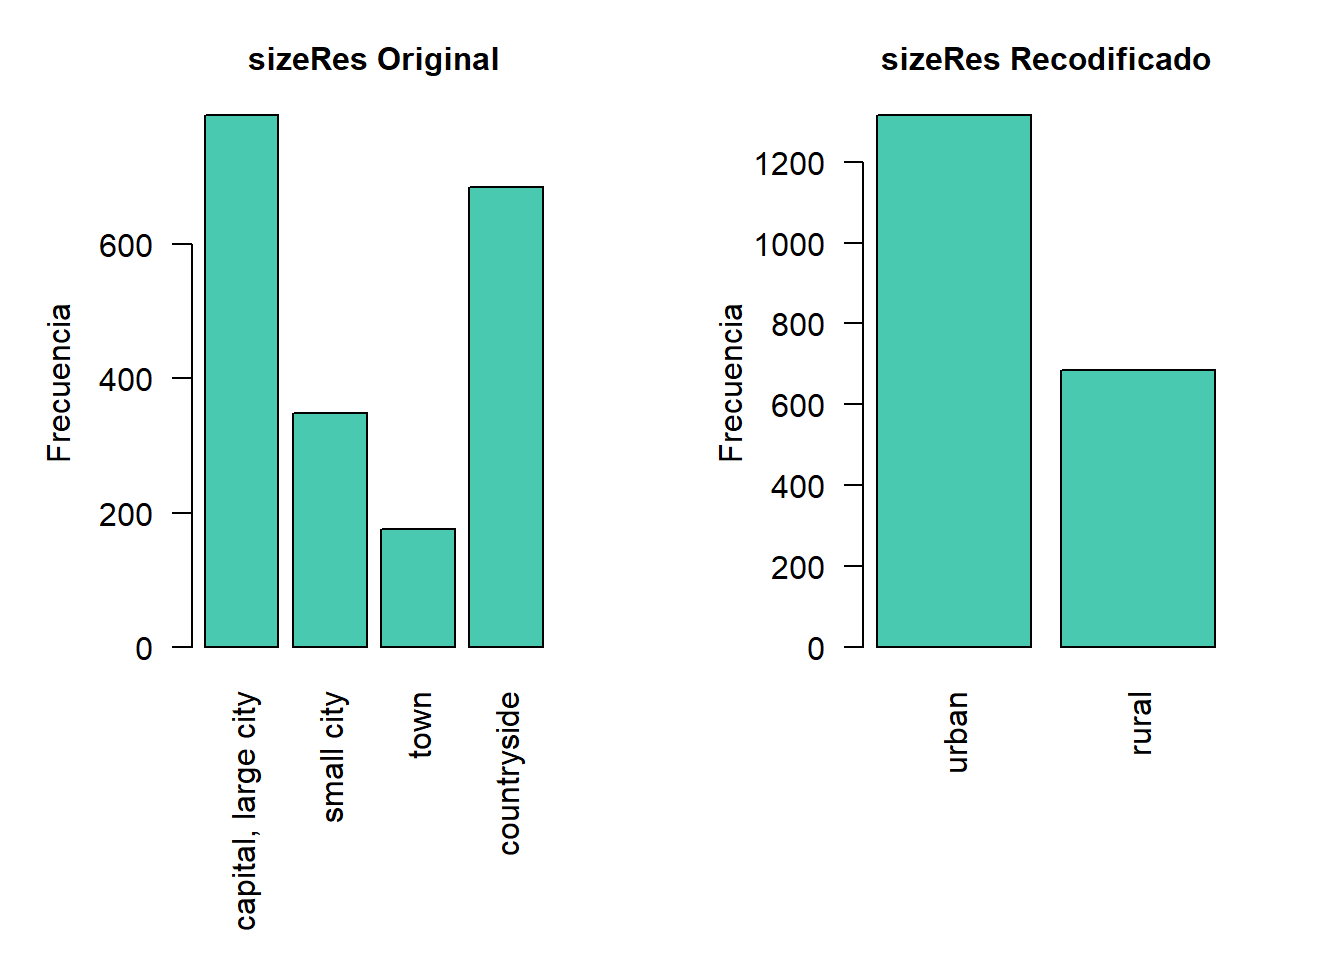
\includegraphics[width=1\linewidth]{bookdown-demo_files/figure-latex/fig4-1} \caption{Efecto de la recodificación y recuentos de frecuencia antes y después de la recodificación}\label{fig:fig4}
\end{figure}

\hypertarget{recodificaciuxf3n-de-una-variable-continua-mediante-la-funciuxf3n-sdcmicro-globalrecode}{%
\paragraph{\texorpdfstring{Recodificación de una variable continua mediante la función \texttt{sdcMicro}: \texttt{globalRecode()}}{Recodificación de una variable continua mediante la función sdcMicro: globalRecode()}}\label{recodificaciuxf3n-de-una-variable-continua-mediante-la-funciuxf3n-sdcmicro-globalrecode}}

La recodificación global de las variables numéricas (continuas) puede lograrse en \texttt{sdcMicro} utilizando la función \texttt{globalRecode()}, que permite especificar un vector con los puntos de quiebre entre los intervalos. La recodificación de una variable continua la convierte en una variable categórica. Además, se puede especificar un vector de etiquetas para las nuevas categorías. Por defecto, las etiquetas son los intervalos, por ejemplo, ``(0, 10{]}''. El Bloque \ref{exm:bloque16jgm} muestra cómo recodificar la variable edad en intervalos de 10 años para valores de edad entre 0 y 100.

\begin{quote}
\textbf{Nota}: A los valores que quedan fuera de los intervalos especificados se les asigna un valor perdido \texttt{NA}
\end{quote}

Por lo tanto, los intervalos deben cubrir todo el rango de valores de la variable.

\begin{example}
\protect\hypertarget{exm:bloque16jgm}{}\label{exm:bloque16jgm}Uso de la función \texttt{sdcMicro} \texttt{globalRecode()} para recodificar una variable continua (edad)
\end{example}

\begin{Shaded}
\begin{Highlighting}[]
\NormalTok{sdcInitial }\OtherTok{\textless{}{-}} \FunctionTok{globalRecode}\NormalTok{(sdcInitial, }\AttributeTok{column =} \FunctionTok{c}\NormalTok{(}\StringTok{"AGEYRS"}\NormalTok{),}
                           \AttributeTok{breaks =} \DecValTok{10} \SpecialCharTok{*} \FunctionTok{c}\NormalTok{(}\DecValTok{0}\SpecialCharTok{:}\DecValTok{10}\NormalTok{))}

\CommentTok{\# Frecuencias de edad después de recodificar}
\FunctionTok{table}\NormalTok{(sdcInitial}\SpecialCharTok{@}\NormalTok{manipKeyVars}\SpecialCharTok{$}\NormalTok{AGEYRS)}
\end{Highlighting}
\end{Shaded}

\begin{verbatim}
## 
##   (0,10]  (10,20]  (20,30]  (30,40]  (40,50]  (50,60]  (60,70]  (70,80] 
##        0       44      389      578      428      266      173       92 
##  (80,90] (90,100] 
##       27        3
\end{verbatim}

\begin{Shaded}
\begin{Highlighting}[]
\CommentTok{\# Guardo objeto de edad en tramos para volver a utilizar en localSupresion}
\NormalTok{sdcInitial\_edad }\OtherTok{\textless{}{-}}\NormalTok{ sdcInitial}
\end{Highlighting}
\end{Shaded}

\begin{figure}
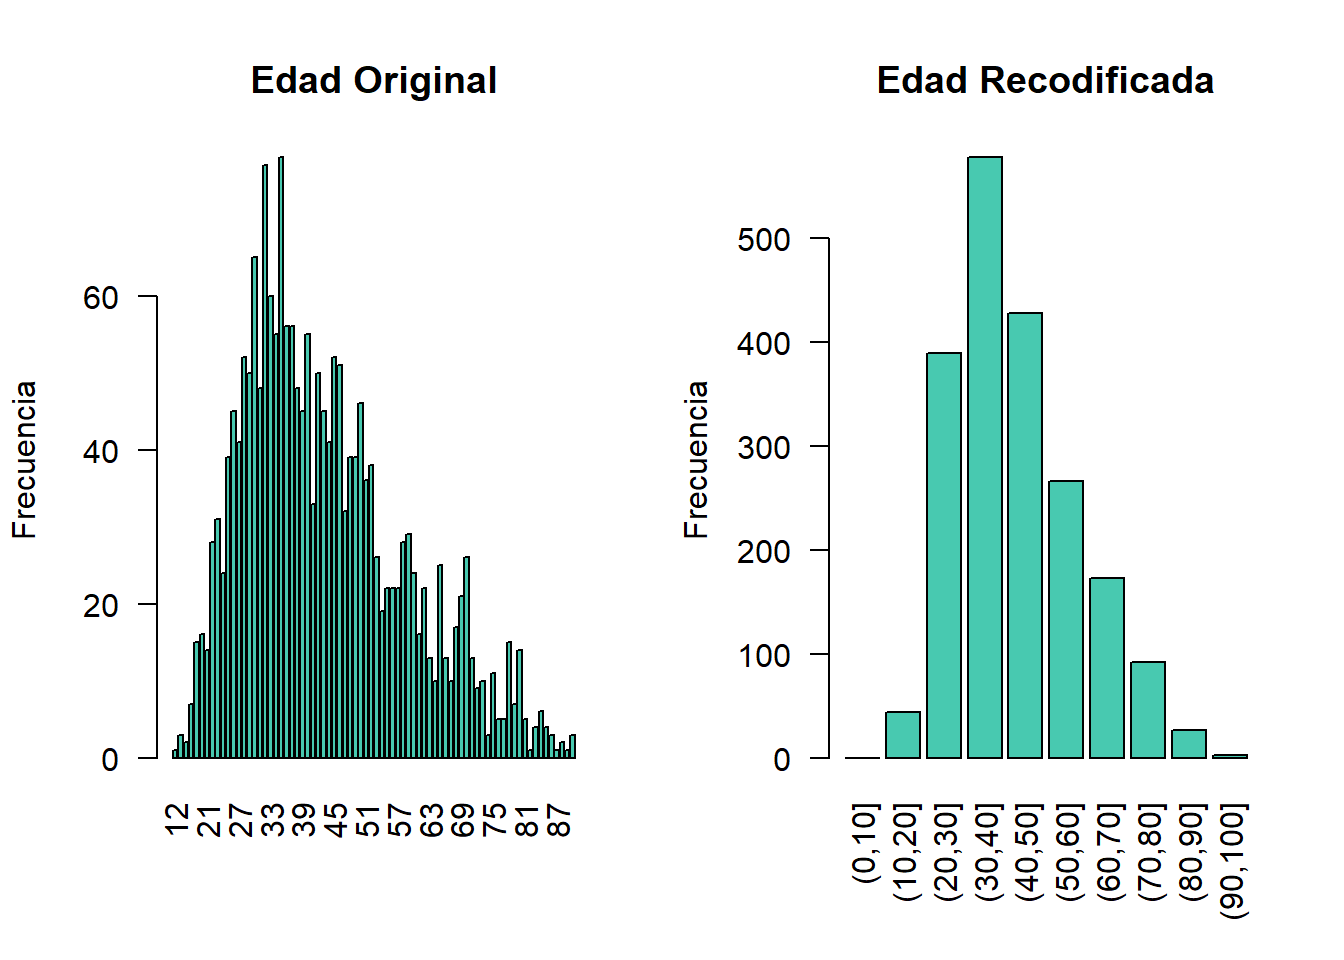
\includegraphics[width=1\linewidth]{bookdown-demo_files/figure-latex/fig5-1} \caption{Variable de edad antes y después de la recodificación}\label{fig:fig5}
\end{figure}

En lugar de crear intervalos de igual anchura, también podemos crear intervalos de anchura desigual. Esto se ilustra en el Bloque \ref{exm:bloque17jgm}, donde utilizamos los grupos de edad 1-5, 6-11, 12-17, 18-21, 22-25, 26-49, 50-64 y 65+. En este ejemplo, es un paso útil, ya que incluso después de recodificar en intervalos de 10 años, las categorías con valores de edad altos tienen frecuencias bajas. Elegimos los intervalos respetando los valores relevantes de la edad escolar y de la edad laboral (por ejemplo, la edad de jubilación es de 65 años en este ejemplo) de forma que los datos puedan seguir utilizándose para la investigación común sobre educación y empleo. La \ref{fig:fig6} muestra el efecto de la recodificación de la variable ``edad''.

\begin{example}
\protect\hypertarget{exm:bloque17jgm}{}\label{exm:bloque17jgm}Uso de \texttt{globalRecode()} para crear intervalos de ancho desigual
\end{example}

\begin{Shaded}
\begin{Highlighting}[]
\NormalTok{sdcInitial }\OtherTok{\textless{}{-}} \FunctionTok{undolast}\NormalTok{(sdcInitial)}

\NormalTok{sdcInitial }\OtherTok{\textless{}{-}} \FunctionTok{globalRecode}\NormalTok{(sdcInitial, }\AttributeTok{column =} \FunctionTok{c}\NormalTok{(}\StringTok{"AGEYRS"}\NormalTok{),}
                           \AttributeTok{breaks =} \FunctionTok{c}\NormalTok{(}\DecValTok{0}\NormalTok{, }\DecValTok{5}\NormalTok{, }\DecValTok{11}\NormalTok{, }\DecValTok{17}\NormalTok{, }\DecValTok{21}\NormalTok{, }\DecValTok{25}\NormalTok{, }\DecValTok{49}\NormalTok{, }\DecValTok{65}\NormalTok{, }\DecValTok{100}\NormalTok{))}

\CommentTok{\# Frecuencias de edad después de recodificar}
\FunctionTok{table}\NormalTok{(sdcInitial}\SpecialCharTok{@}\NormalTok{manipKeyVars}\SpecialCharTok{$}\NormalTok{AGEYRS)}
\end{Highlighting}
\end{Shaded}

\begin{verbatim}
## 
##    (0,5]   (5,11]  (11,17]  (17,21]  (21,25]  (25,49]  (49,65] (65,100] 
##        0        0        6       52      122     1213      398      209
\end{verbatim}

\begin{figure}
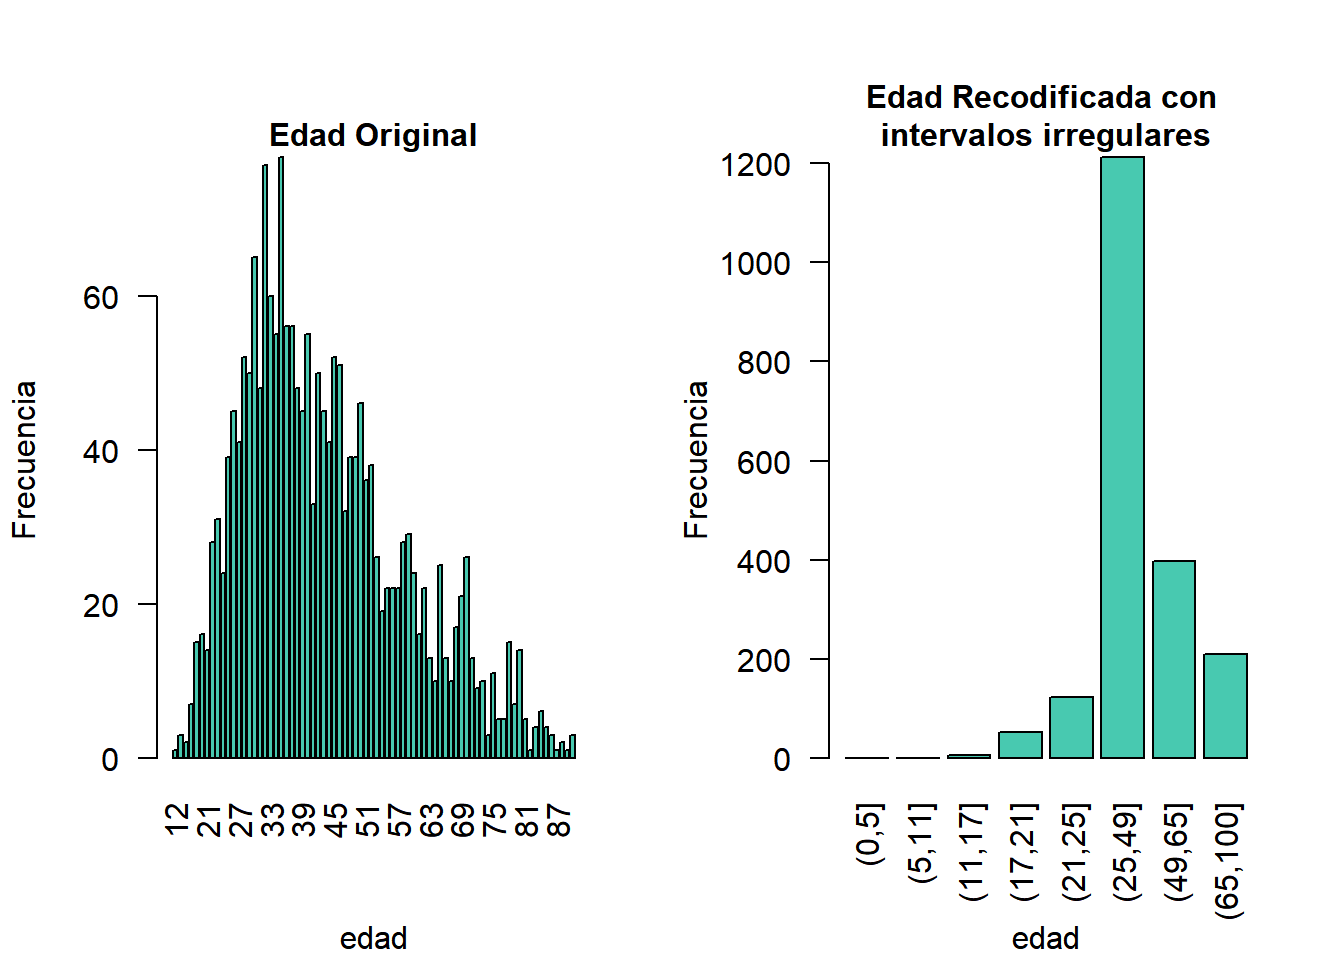
\includegraphics[width=1\linewidth]{bookdown-demo_files/figure-latex/fig6-1} \caption{Variable de edad antes y después de la recodificación}\label{fig:fig6}
\end{figure}

Precaución sobre el uso de la función \texttt{globalRecode()} en \texttt{sdcMicro}: En la implementación actual de \texttt{sdcMicro}, los intervalos se definen como abiertos a la izquierda. En términos matemáticos, esto significa que, en nuestro ejemplo, la edad 0 está excluida de los intervalos especificados. En notación de intervalos, esto se denota como (0, 5{]} (como en las etiquetas del eje x en la \ref{fig:fig5} y la \ref{fig:fig6} para la variable recodificada). El intervalo (0, 5{]} se interpreta como de 0 a 5 y no incluye el 0, pero sí el 5. \texttt{R} recodifica los valores que no están contenidos en ninguno de los intervalos como perdidos (\texttt{NA}). Esta implementación establecería en nuestro ejemplo todos los valores de edad 0 (niños menores de 1 año) como perdidos y podría significar potencialmente una gran pérdida de datos. La función \texttt{globalRecode()} solo permite construir intervalos que queden abiertos. Este puede no ser un resultado deseable y la pérdida de las edades cero de los datos es claramente problemática para un conjunto de datos del mundo real.

Para construir intervalos abiertos a la derecha, por ejemplo, en nuestro ejemplo, para los intervalos de edad {[}0,14), {[}15, 65), {[}66, 100), presentamos dos alternativas de recodificación global:

\begin{itemize}
\tightlist
\item
  Una solución para las variables semicontinuas\footnote{Este enfoque sólo funciona para variables semicontinuas, porque en el caso de las variables continuas, puede haber valores que se encuentren entre el límite inferior del intervalo y el límite inferior del intervalo menos el número menor. Por ejemplo, utilizando este método para los ingresos, tendríamos un intervalo (9999, 19999} y el valor 9999,5 se clasificaría erróneamente como perteneciente al intervalo {[}10000, 19999{]}.{]} que permitiría utilizar \texttt{globalRecode()} sería restar un pequeño número a los intervalos límite, permitiendo así crear los intervalos deseados. En el siguiente ejemplo, restar 0,1 a cada intervalo obliga a \texttt{globalRecode()} a incluir el 0 en el intervalo inferior y permitir las pausas donde las queramos. Establecemos el límite superior del intervalo para que sea mayor que el valor máximo de la variable ``edad''. Podemos utilizar la opción etiquetas para definir etiquetas claras para las nuevas categorías. Esto se ilustra en el Bloque \ref{exm:bloque18jgm}.
\end{itemize}

\begin{example}
\protect\hypertarget{exm:bloque18jgm}{}\label{exm:bloque18jgm}Construcción de intervalos abiertos a la derecha para variables semicontinuas utilizando la función incorporada de \texttt{sdcMicro}, \texttt{globalRecode()}
\end{example}

\begin{Shaded}
\begin{Highlighting}[]
\NormalTok{sdcInitial }\OtherTok{\textless{}{-}} \FunctionTok{undolast}\NormalTok{(sdcInitial)}

\NormalTok{sdcInitial }\OtherTok{\textless{}{-}} \FunctionTok{globalRecode}\NormalTok{(sdcInitial, }\AttributeTok{column =} \FunctionTok{c}\NormalTok{(}\StringTok{"AGEYRS"}\NormalTok{),}
                           \AttributeTok{breaks =} \FunctionTok{c}\NormalTok{(}\SpecialCharTok{{-}}\FloatTok{0.1}\NormalTok{, }\FloatTok{14.9}\NormalTok{, }\FloatTok{64.9}\NormalTok{, }\FloatTok{99.9}\NormalTok{),}
                           \AttributeTok{labels =} \FunctionTok{c}\NormalTok{(}\StringTok{\textquotesingle{}[0,15)\textquotesingle{}}\NormalTok{, }\StringTok{\textquotesingle{}[15,65)\textquotesingle{}}\NormalTok{, }\StringTok{\textquotesingle{}[65,100)\textquotesingle{}}\NormalTok{))}
\end{Highlighting}
\end{Shaded}

\begin{figure}
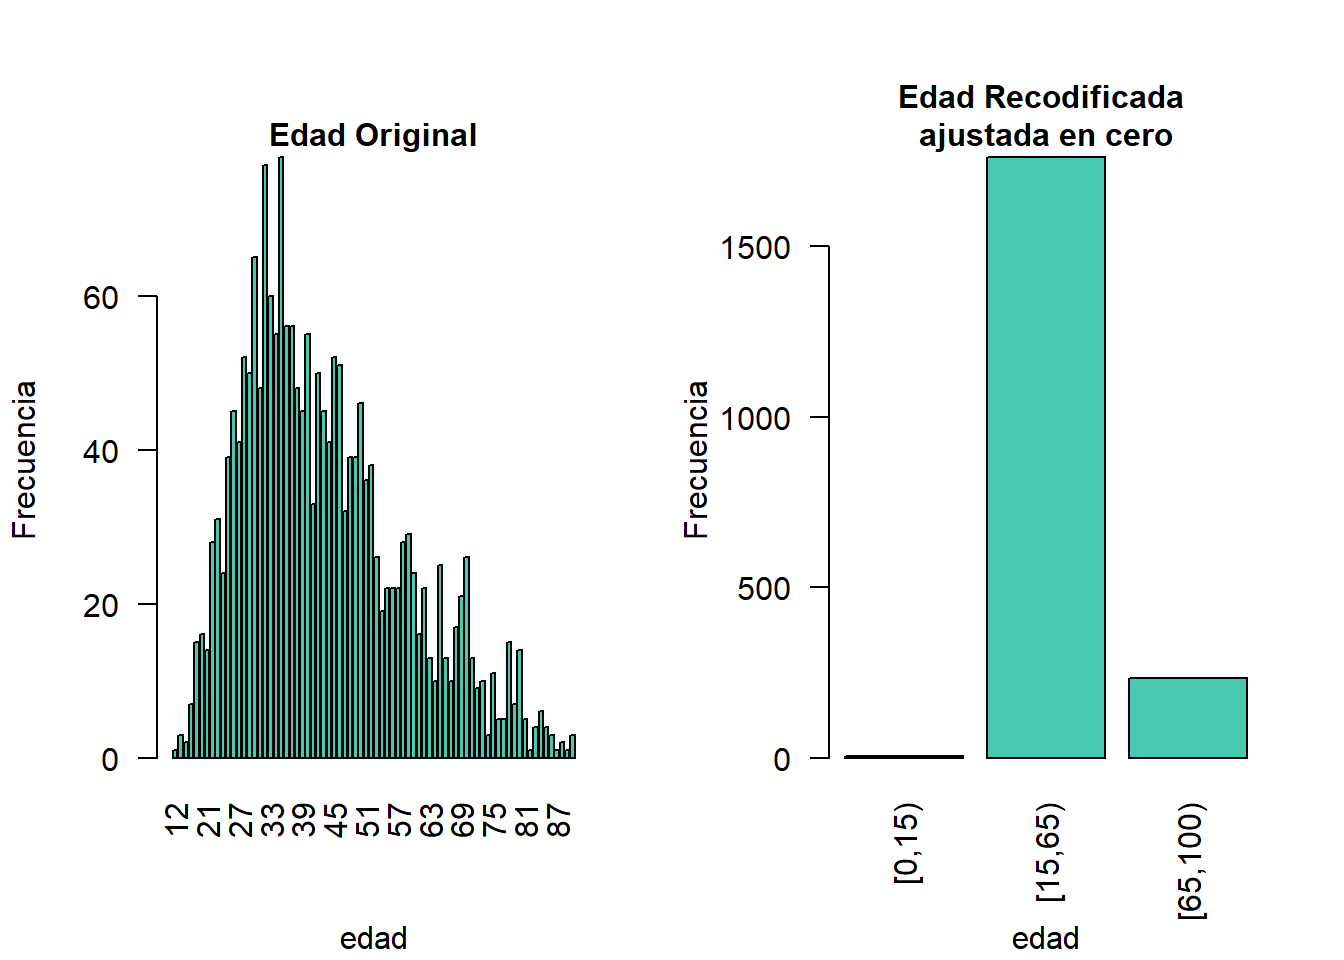
\includegraphics[width=1\linewidth]{bookdown-demo_files/figure-latex/figx1-1} \caption{Variable de edad antes y después de la recodificación}\label{fig:figx1}
\end{figure}

\begin{itemize}
\tightlist
\item
  También es posible utilizar código en \texttt{R} para recodificar manualmente las variables sin utilizar las funciones \texttt{sdcMicro}. Cuando se utilizan las funciones \texttt{sdcMicro}, el cambio en el riesgo después de la recodificación se recalcula automáticamente, pero si se recodifica manualmente no lo hace. En este caso, hay que dar un paso más y recalcular el riesgo después de cambiar manualmente las variables en el objeto \texttt{sdcMicro}. Este enfoque también es válido para las variables continuas y se ilustra en el Bloque \ref{exm:bloque19jgm}.
\end{itemize}

\begin{example}
\protect\hypertarget{exm:bloque19jgm}{}\label{exm:bloque19jgm}Construcción de intervalos para variables semicontinuas y continuas mediante recodificación manual en R
\end{example}

\begin{Shaded}
\begin{Highlighting}[]
\NormalTok{sdcInitial }\OtherTok{\textless{}{-}} \FunctionTok{undolast}\NormalTok{(sdcInitial)}

\CommentTok{\# Grupo edad 0{-}14}
\NormalTok{sdcInitial}\SpecialCharTok{@}\NormalTok{manipKeyVars}\SpecialCharTok{$}\NormalTok{AGEYRS[sdcInitial}\SpecialCharTok{@}\NormalTok{manipKeyVars}\SpecialCharTok{$}\NormalTok{AGEYRS }\SpecialCharTok{\textgreater{}=} \DecValTok{0} \SpecialCharTok{\&}
\NormalTok{sdcInitial}\SpecialCharTok{@}\NormalTok{manipKeyVars}\SpecialCharTok{$}\NormalTok{AGEYRS }\SpecialCharTok{\textless{}} \DecValTok{15}\NormalTok{] }\OtherTok{\textless{}{-}} \DecValTok{0}

\CommentTok{\# Grupo edad 15{-}64}
\NormalTok{sdcInitial}\SpecialCharTok{@}\NormalTok{manipKeyVars}\SpecialCharTok{$}\NormalTok{AGEYRS[sdcInitial}\SpecialCharTok{@}\NormalTok{manipKeyVars}\SpecialCharTok{$}\NormalTok{AGEYRS }\SpecialCharTok{\textgreater{}=} \DecValTok{15} \SpecialCharTok{\&}
\NormalTok{sdcInitial}\SpecialCharTok{@}\NormalTok{manipKeyVars}\SpecialCharTok{$}\NormalTok{AGEYRS }\SpecialCharTok{\textless{}} \DecValTok{65}\NormalTok{] }\OtherTok{\textless{}{-}} \DecValTok{1}

\CommentTok{\# Grupo edad 65{-}100}
\NormalTok{sdcInitial}\SpecialCharTok{@}\NormalTok{manipKeyVars}\SpecialCharTok{$}\NormalTok{AGEYRS[sdcInitial}\SpecialCharTok{@}\NormalTok{manipKeyVars}\SpecialCharTok{$}\NormalTok{AGEYRS }\SpecialCharTok{\textgreater{}=} \DecValTok{65} \SpecialCharTok{\&}
\NormalTok{sdcInitial}\SpecialCharTok{@}\NormalTok{manipKeyVars}\SpecialCharTok{$}\NormalTok{AGEYRS }\SpecialCharTok{\textless{}=} \DecValTok{100}\NormalTok{] }\OtherTok{\textless{}{-}} \DecValTok{2}

\CommentTok{\# Añadir etiquetas para los nuevos valores}
\NormalTok{sdcInitial}\SpecialCharTok{@}\NormalTok{manipKeyVars}\SpecialCharTok{$}\NormalTok{AGEYRS }\OtherTok{\textless{}{-}}\FunctionTok{ordered}\NormalTok{(sdcInitial}\SpecialCharTok{@}\NormalTok{manipKeyVars}\SpecialCharTok{$}\NormalTok{AGEYRS,}
\AttributeTok{levels =} \FunctionTok{c}\NormalTok{(}\DecValTok{0}\NormalTok{,}\DecValTok{1}\NormalTok{,}\DecValTok{2}\NormalTok{), }\AttributeTok{labels =} \FunctionTok{c}\NormalTok{(}\StringTok{"0{-}14"}\NormalTok{, }\StringTok{"15{-}64"}\NormalTok{, }\StringTok{"65{-}100"}\NormalTok{))}

\CommentTok{\# Recalcular el riesgo tras una transformación manual}
\NormalTok{sdcInitial }\OtherTok{\textless{}{-}} \FunctionTok{calcRisks}\NormalTok{(sdcInitial)}
\end{Highlighting}
\end{Shaded}

\hypertarget{cod-sup-inf}{%
\subsubsection{Codificación superior e inferior}\label{cod-sup-inf}}

La codificación superior e inferior es similar a la recodificación global, pero en lugar de recodificar todos los valores, solo se recodifican los valores superiores y/o inferiores de la distribución o las categorías. Esto solo puede aplicarse a las variables categóricas ordinales y a las variables semi-continuas, ya que los valores tienen que estar al menos ordenados. La codificación superior e inferior es especialmente útil si el grueso de los valores se encuentra en el centro de la distribución y las categorías periféricas tienen pocas observaciones (valores atípicos). Los ejemplos son la edad y los ingresos; para estas variables, a menudo habrá solo unas pocas observaciones por encima de ciertos umbrales, normalmente en las colas de la distribución. Cuanto menor sea el número de observaciones dentro de una categoría, mayor será el riesgo de identificación. Una solución podría ser agrupar los valores de las colas de la distribución en una categoría. Esto reduce el riesgo para esas observaciones y, lo que es más importante, lo hace sin reducir la utilidad de los datos para las demás observaciones de la distribución.

Decidir dónde aplicar el umbral y qué observaciones deben agruparse requiere:

\begin{itemize}
\tightlist
\item
  Revisar la distribución global de la variable para identificar en qué punto las frecuencias caen por debajo del número deseado de observaciones e identificar los valores atípicos en la distribución. \ref{fig:fig7} muestra la distribución de la variable edad y sugiere 65 (línea vertical roja) para el código superior de edad.
\item
  Tener en cuenta el uso previsto de los datos y el propósito para el que se realizó la encuesta. Por ejemplo, si los datos se utilizan normalmente para medir la participación en la fuerza laboral de las personas de 15 a 64 años, la codificación superior e inferior no debe interferir con las categorías de 15 a 64 años. De lo contrario, el analista se encontraría con la imposibilidad de crear las medidas deseadas para las que estaban destinados los datos. En el ejemplo, consideramos esto y codificamos todas las edades superiores a 64 años.
\end{itemize}

\begin{figure}
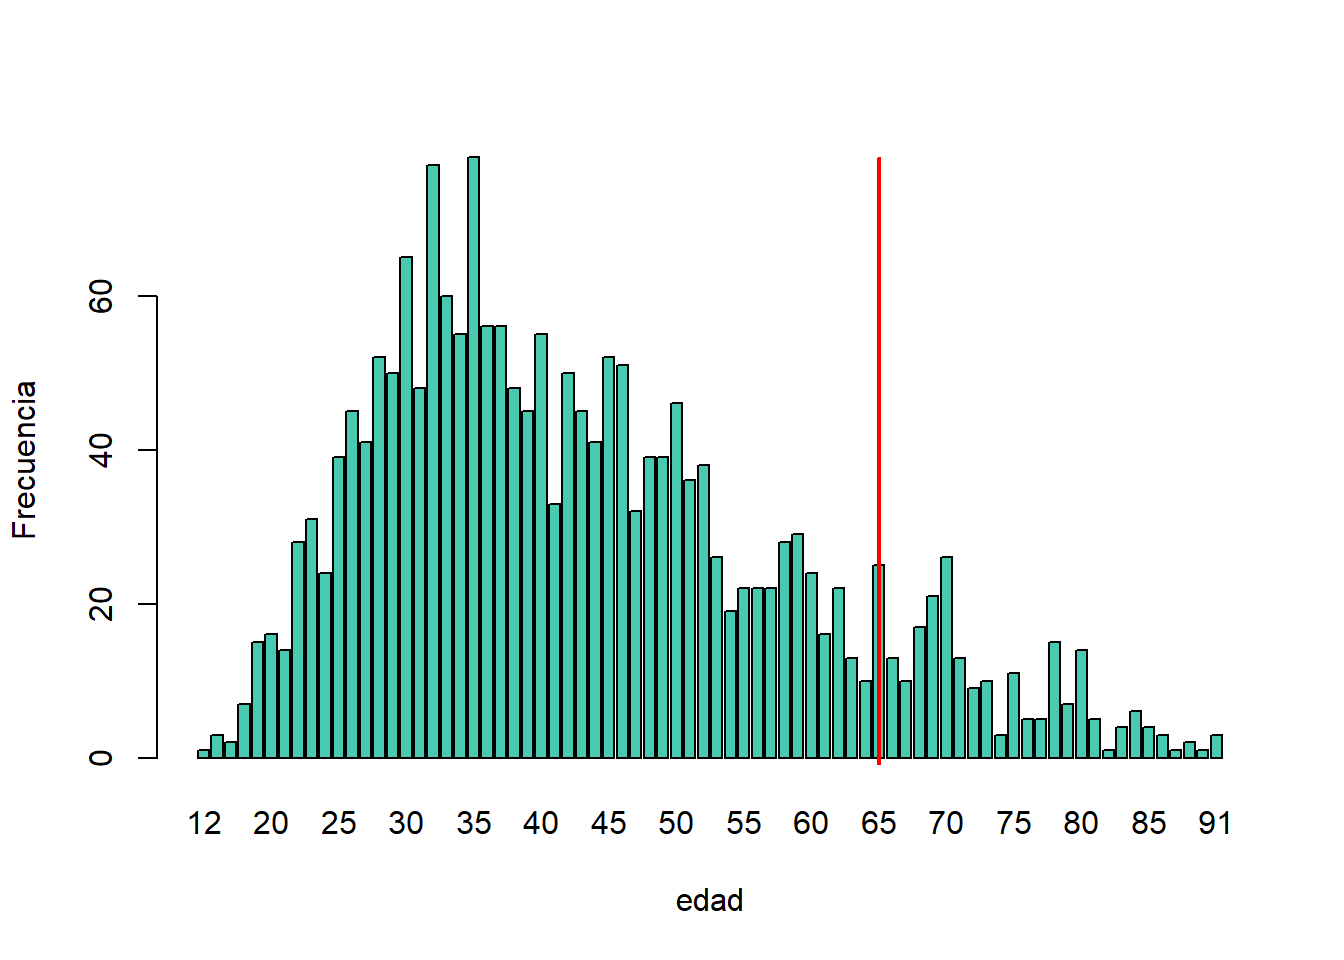
\includegraphics[width=1\linewidth]{bookdown-demo_files/figure-latex/fig7-1} \caption{Utilización de la distribución de frecuencias de la variable edad para determinar el umbral de la codificación superior}\label{fig:fig7}
\end{figure}

La codificación superior e inferior se puede hacer fácilmente con la función \texttt{topBotCoding()} en \texttt{sdcMicro}. La codificación superior y la inferior no pueden hacerse simultáneamente en \texttt{sdcMicro}. El Bloque \ref{exm:bloque20jgm} ilustra cómo recodificar valores de edad superior a 64 y valores de edad inferior a 5; 65 y 5 reemplazan los valores respectivamente. Para construir varias categorías de codificación superior o inferior, por ejemplo, edad de 65 a 80 años y superior a 80 años, se puede utilizar la función \texttt{groupAndRename()} en sdcMicro o la recodificación manual como se describe en la subsección anterior.

\begin{example}
\protect\hypertarget{exm:bloque20jgm}{}\label{exm:bloque20jgm}Codificación superior y codificación inferior en \texttt{sdcMicro} utilizando la función \texttt{topBotCoding()}
\end{example}

\begin{Shaded}
\begin{Highlighting}[]
\NormalTok{sdcInitial }\OtherTok{\textless{}{-}}\NormalTok{ sdc\_respaldo }\CommentTok{\# leo nuevamente la Tabla}

\CommentTok{\# Top coding en edad 65}
\NormalTok{sdcInitial }\OtherTok{\textless{}{-}} \FunctionTok{topBotCoding}\NormalTok{(}\AttributeTok{obj =}\NormalTok{ sdcInitial, }\AttributeTok{value =} \DecValTok{65}\NormalTok{, }\AttributeTok{replacement =} \DecValTok{65}\NormalTok{,}
                           \AttributeTok{kind =} \StringTok{"top"}\NormalTok{, }\AttributeTok{column =} \StringTok{"AGEYRS"}\NormalTok{)}

\CommentTok{\# Bottom coding en edad 5}
\NormalTok{sdcInitial }\OtherTok{\textless{}{-}} \FunctionTok{topBotCoding}\NormalTok{(}\AttributeTok{obj =}\NormalTok{ sdcInitial, }\AttributeTok{value =} \DecValTok{5}\NormalTok{, }\AttributeTok{replacement =} \DecValTok{5}\NormalTok{,}
                           \AttributeTok{kind =} \StringTok{"bottom"}\NormalTok{, }\AttributeTok{column =} \StringTok{"AGEYRS"}\NormalTok{)}

\CommentTok{\#table(sdcInitial@manipKeyVars$AGEYRS)}
\end{Highlighting}
\end{Shaded}

\begin{figure}
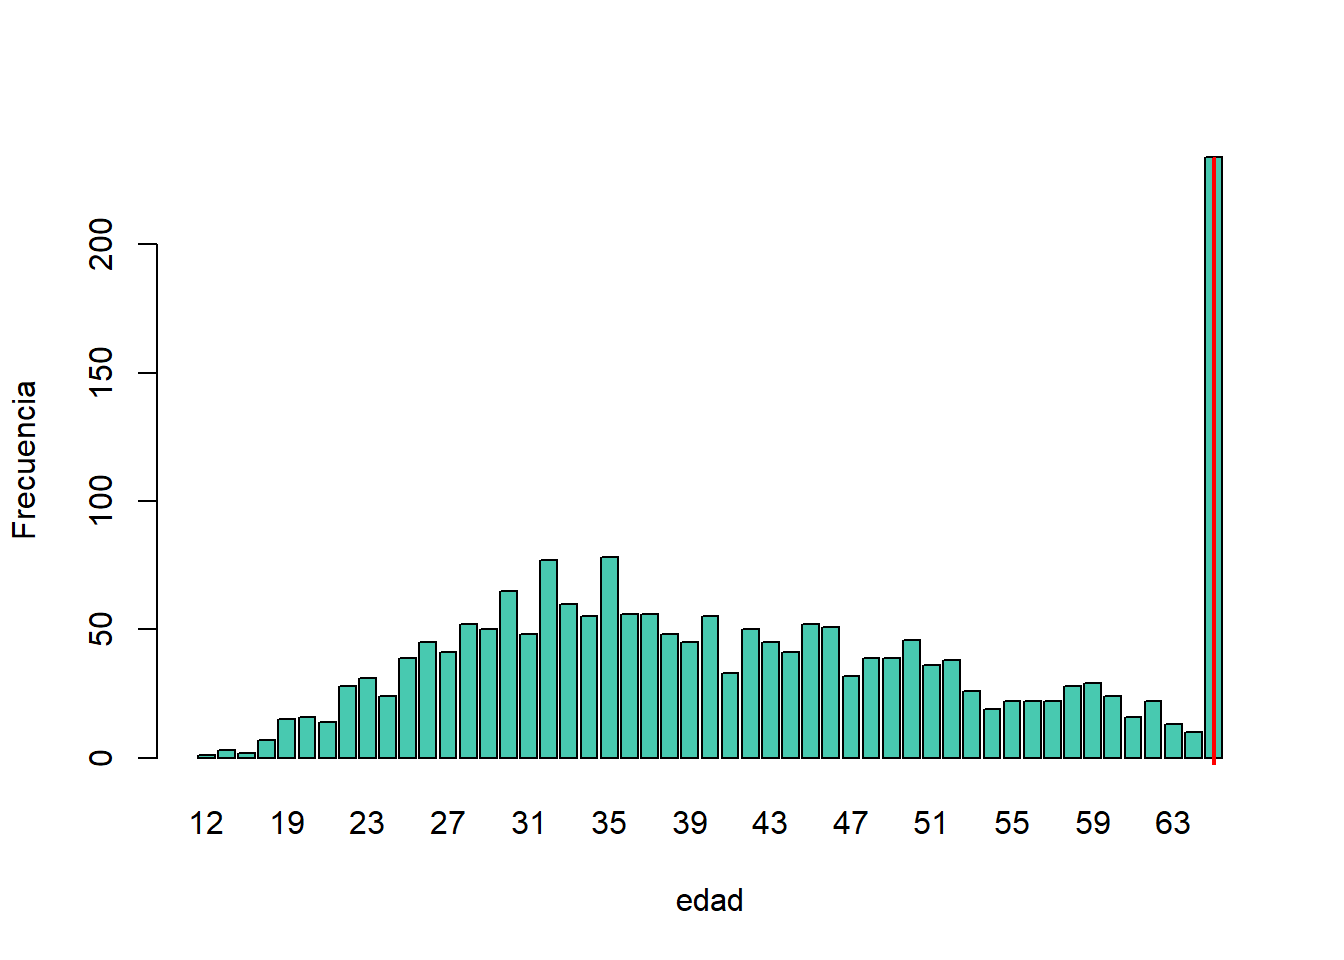
\includegraphics[width=1\linewidth]{bookdown-demo_files/figure-latex/figx2-1} \caption{Distribución de frecuencias de la variable edad con codificación superior}\label{fig:figx2}
\end{figure}

\hypertarget{redondeo}{%
\subsubsection{Redondeo}\label{redondeo}}

El redondeo es similar a la agrupación, pero se utiliza para las variables continuas. El redondeo es útil para evitar la coincidencia exacta con fuentes de datos externas. Además, puede utilizarse para reducir el nivel de detalle de los datos. Algunos ejemplos son la eliminación de las cifras decimales o el redondeo a la unidad más cercana.

\begin{Shaded}
\begin{Highlighting}[]
\NormalTok{sdcInitial }\OtherTok{\textless{}{-}}\NormalTok{ sdc\_respaldo }\CommentTok{\# leo nuevamente la Tabla}

\FunctionTok{table}\NormalTok{(sdcInitial}\SpecialCharTok{@}\NormalTok{manipKeyVars}\SpecialCharTok{$}\NormalTok{AGEYRS)}
\end{Highlighting}
\end{Shaded}

\begin{verbatim}
## 
## 12 14 17 18 19 20 21 22 23 24 25 26 27 28 29 30 31 32 33 34 35 36 37 38 39 40 
##  1  3  2  7 15 16 14 28 31 24 39 45 41 52 50 65 48 77 60 55 78 56 56 48 45 55 
## 41 42 43 44 45 46 47 48 49 50 51 52 53 54 55 56 57 58 59 60 61 62 63 64 65 66 
## 33 50 45 41 52 51 32 39 39 46 36 38 26 19 22 22 22 28 29 24 16 22 13 10 25 13 
## 67 68 69 70 71 72 73 74 75 76 77 78 79 80 81 82 83 84 85 86 87 88 90 91 
## 10 17 21 26 13  9 10  3 11  5  5 15  7 14  5  1  4  6  4  3  1  2  1  3
\end{verbatim}

\begin{Shaded}
\begin{Highlighting}[]
\CommentTok{\# Se redondea a la decena más cercana}
\NormalTok{sdcInitial}\SpecialCharTok{@}\NormalTok{manipKeyVars}\SpecialCharTok{$}\NormalTok{AGEYRS }\OtherTok{\textless{}{-}} \FunctionTok{round}\NormalTok{(sdcInitial}\SpecialCharTok{@}\NormalTok{manipKeyVars}\SpecialCharTok{$}\NormalTok{AGEYRS,}\SpecialCharTok{{-}}\DecValTok{1}\NormalTok{)}

\FunctionTok{table}\NormalTok{(sdcInitial}\SpecialCharTok{@}\NormalTok{manipKeyVars}\SpecialCharTok{$}\NormalTok{AGEYRS)}
\end{Highlighting}
\end{Shaded}

\begin{verbatim}
## 
##  10  20  30  40  50  60  70  80  90 
##   4 176 493 559 326 233 122  77  10
\end{verbatim}

En la siguiente sección se analiza el método de supresión local. La recodificación suele utilizarse antes de la supresión local para reducir el número de supresiones necesarias.

\begin{quote}
Lectura recomendada de recodificación:
- Hundepool, Anco, Josep Domingo-Ferrer, Luisa Franconi, Sarah Giessing, Rainer Lenz, Jane Naylor, Eric Schulte Nordholt, Giovanni Seri, and Peter Paul de Wolf. 2006. Handbook on Statistical Disclosure Control. ESSNet SDC. \url{http://neon.vb.cbs.nl/casc/handbook.htm}.
- Hundepool, Anco, Josep Domingo-Ferrer, Luisa Franconi, Sarah Giessing, Eric Schulte Nordholt, Keith Spicer, and Peter Paul de Wolf. 2012. Statistical Disclosure Control. Chichester: John Wiley \& Sons Ltd.~\url{doi:10.1002/9781118348239}.
- Templ, Matthias, Bernhard Meindl, Alexander Kowarik, and Shuang Chen. 2014. Statistical Disclosure Control (SDCMicro). \url{http://www.ihsn.org/home/software/disclosure-control-toolbox}. (accessed June 9, 2018).
- De Waal, A.G., and Willenborg, L.C.R.J. 1999. Information loss through global recoding and local suppression. Netherlands Official Statistics, 14:17-20, 1999. Special issue on SDC
\end{quote}

\hypertarget{sup-loc}{%
\subsection{Supresión local}\label{sup-loc}}

En las encuestas es frecuente encontrar valores para ciertas variables o combinaciones de identificadores indirectos que son compartidos por muy pocos individuos. Cuando esto ocurre, el riesgo de reidentificación para esos encuestados es mayor que para el resto de los encuestados (véase la sección \protect\hyperlink{k-anonimato}{k-anonimato}). A menudo se utiliza la supresión local tras reducir el número de claves en los datos al recodificar las variables adecuadas. La recodificación reduce el número de supresiones necesarias, así como el tiempo de cálculo para la supresión. La supresión de valores significa que los valores de una variable se sustituyen por un valor ausente \texttt{NA} en \texttt{R}). En la sección \protect\hyperlink{k-anonimato}{k-anonimato} se analiza cómo influyen los valores perdidos en los recuentos de frecuencia y en el \(k\)-anonimato. Es importante tener en cuenta que no se suprimen todos los valores de todos los individuos de una determinada variable, lo que ocurriría al eliminar un identificador directo, como el ``nombre''; solo se suprimen determinados valores de una variable concreta y de un encuestado o conjunto de encuestados concreto. Esto se ilustra en el siguiente ejemplo y en la Tabla \ref{tab:Tabla9}.

La Tabla \ref{tab:Tabla9} presenta un conjunto de datos con siete encuestados y tres identificadores indirectos. La combinación \{``mujer'', ``rural'', ``superior''\} para las variables ``sexo'', ``región'' y ``educación'' es una combinación poco segura, ya que es única en la muestra. Al suprimir el valor ``mujer'' o ``superior'', el encuestado ya no puede distinguirse de los demás encuestados, ya que ese encuestado comparte la misma combinación de variables clave con al menos otros tres encuestados. Solo se suprime el valor de la combinación insegura del único encuestado en riesgo, no los valores de la misma variable de los demás encuestados. La libertad de elegir qué valor se suprime puede utilizarse para minimizar el número total de supresiones y, por tanto, la pérdida de información. Además, si una variable es muy importante para el usuario, podemos elegir no suprimir los valores de esta variable, a menos que sea estrictamente necesario. En el ejemplo, podemos elegir entre suprimir el valor ``mujer'' o ``mayor'' para conseguir un archivo de datos seguro; elegimos suprimir ``mayor''. Esta elección debe hacerse teniendo en cuenta las necesidades de los usuarios de los datos. En este ejemplo, consideramos que ``sexo'' es más importante que ``educación''.

\begin{table}

\caption{\label{tab:Tabla9}\label{tab:Tabla9}Ilustración de la supresión local - datos antes y después de la supresión}
\centering
\begin{tabular}[t]{clllcll}
\toprule
\multicolumn{4}{c}{Datos originales} & \multicolumn{3}{c}{Después de supresión local} \\
\cmidrule(l{3pt}r{3pt}){1-4} \cmidrule(l{3pt}r{3pt}){5-7}
ID & Sexo & Zona & Educación & Sexo & Zona & Educación\\
\midrule
1 & mujer & rural & superior & mujer & rural & NA / perdido\\
2 & hombre & rural & superior & hombre & rural & superior\\
3 & hombre & rural & superior & hombre & rural & superior\\
4 & hombre & rural & superior & hombre & rural & superior\\
5 & mujer & rural & media & mujer & rural & media\\
\addlinespace
6 & mujer & rural & media & mujer & rural & media\\
7 & mujer & rural & media & mujer & rural & media\\
\bottomrule
\end{tabular}
\end{table}

Dado que las variables continuas tienen un elevado número de valores únicos (por ejemplo, los ingresos en dólares o la edad en años), el \(k\)-anonimato y la supresión local no son adecuadas para las variables continuas o las variables con un número muy elevado de categorías. Una posible solución en esos casos podría ser recodificar primero para producir menos categorías (por ejemplo, recodificar la edad en intervalos de 10 años o los ingresos en quintiles). No obstante, \textbf{tenga siempre presente el efecto que tendrá cualquier recodificación en la utilidad de los datos}.

El paquete \texttt{sdcMicro} incluye dos funciones para la supresión local: \texttt{localSuppression()} y \texttt{localSupp()}. La función \texttt{localSuppression()} es la más utilizada y permite el uso de la supresión en identificadores indirectos especificados para lograr un cierto nivel de \(k\)-anonimato para estos identificadores indirectos. El algoritmo utilizado busca minimizar el número total de supresiones mientras se alcanza el umbral de \(k\)-anonimato requerido. Por defecto, el algoritmo tiene más probabilidades de suprimir valores de variables con muchas categorías o valores diferentes, y menos de suprimir variables con menos categorías. Por ejemplo, es más probable que se supriman los valores de una variable geográfica, con 12 áreas diferentes, que los valores de la variable ``sexo'', que suele tener solo dos categorías. Si las variables con muchos valores diferentes son importantes para la utilidad de los datos y no se desea la supresión para ellas, es posible clasificar las variables por importancia en la función \texttt{localSuppression()} y así especificar el orden en el que el algoritmo tratará de suprimir los valores dentro de los identificadores indirectos para lograr el \(k\)-anonimato. El algoritmo trata de aplicar menos supresiones a las variables de gran importancia que a las de menor importancia. Sin embargo, las supresiones en las variables con alta importancia pueden ser inevitables para lograr el nivel requerido de \(k\)-anonimato.

En el Bloque \ref{exm:bloque21jgm}, se aplica la supresión local para alcanzar el umbral de \(k\)-anonimato de 5 en los identificadores indirectos ``sexo'', ``región'', ``religión'', ``edad'' y ``etnia''\footnote{Aquí, el objeto \texttt{sdcMicro} ``sdcIntial'' contiene un conjunto de datos con 2.500 individuos y 103 variables. Seleccionamos cinco identificadores indirectos: ``sizeRes'', ``edad'', ``sexo'', ``región'' y ``etnia''.}. Sin clasificar la importancia de las variables, el valor de la variable ``edad'' es más probable que se suprima, ya que es la variable con más categorías. La variable ``edad'' tiene 10 categorías después de la recodificación. La variable ``sexo'' es la menos probable que se suprima, ya que solo tiene dos valores diferentes: ``hombre'' y ``mujer''. Las demás variables tienen 4 categorías (``tamañoRes''), 2 (``región'') y 8 (``etnia''). Después de aplicar la función localSuppression(), mostramos el número de supresiones por variable con la función incorporada \texttt{print()} con la opción `ls' para la salida de supresión local. Como se esperaba, la variable ``edad'' es la que tiene más supresiones (80). De hecho, solo la variable ``etnia'' de las demás variables también necesitó supresiones (8) para alcanzar el umbral de \(k\)-anonimato de 5. La variable ``etnia'' es la segunda variable con mayor número de supresiones. Posteriormente, deshacemos y rehacemos la supresión local en los mismos datos y reducimos el número de supresiones en ``edad'' especificando el vector de importancia con alta importancia (poca supresión) en el identificador indirecto ``edad''. También,asignamos importancia a la variable ``sexo''. Esto se hace especificando un vector de importancia. Los valores del vector de importancia pueden ir de 1 a \emph{k}, el número de identificadores indirectos. En nuestro ejemplo, \emph{k} es igual a 5. Las variables con valores más bajos en los vectores de importancia tienen una importancia alta y, cuando es posible, reciben menos supresiones que las variables con valores más altos.

Para asignar una importancia alta a las variables ``edad'' y ``sexo'', especificamos el vector de importancia como \texttt{c(5,\ 1,\ 1,\ 4,\ 4,\ 5)}, con el orden según el orden de las variables especificadas en el objeto \texttt{sdcMicro}. El efecto es claro: no hay supresiones en las variables ``edad'' y ``sexo''. En cambio, las demás variables, especialmente ``tamañoRes'' y ``etnia'', recibieron muchas más supresiones. El número total de valores suprimidos ha aumentado de 88 a 166.

\begin{quote}
\textbf{Nota}: Un menor número de supresiones en una variable aumenta el número de supresiones necesarias en otras variables (véase el Bloque \ref{exm:bloque21jgm}).
\end{quote}

Por lo general, el número total de valores suprimidos necesarios para alcanzar el nivel requerido de \(k\)-anonimato aumenta cuando se especifica un vector de importancia, ya que el vector de importancia impide utilizar el patrón de supresión óptimo. El vector de importancia debe especificarse solo en los casos en que las variables con muchas categorías desempeñen un papel importante en la utilidad de los datos para los usuarios de los mismos\footnote{Esto puede evaluarse con medidas de utilidad.}.

\begin{example}
\protect\hypertarget{exm:bloque21jgm}{}\label{exm:bloque21jgm}Aplicación de la supresión local con y sin vector de importancia
\end{example}

\begin{Shaded}
\begin{Highlighting}[]
\CommentTok{\# Se comienza con la edad recodificada en tramos de 10 años}
\NormalTok{sdcInitial }\OtherTok{\textless{}{-}}\NormalTok{ sdcInitial\_edad}
\CommentTok{\#sdcInitial \textless{}{-} sdc\_respaldo \# leo nuevamente la Tabla}
\CommentTok{\#sdcInitial \textless{}{-} undolast(sdcInitial)}

\CommentTok{\# supresión local sin vector de importancia}
\NormalTok{sdcInitial }\OtherTok{\textless{}{-}} \FunctionTok{localSuppression}\NormalTok{(sdcInitial, }\AttributeTok{k =} \DecValTok{2}\NormalTok{)}
\FunctionTok{print}\NormalTok{(sdcInitial, }\AttributeTok{type=}\StringTok{"ls"}\NormalTok{)}
\end{Highlighting}
\end{Shaded}

\begin{verbatim}
## Local suppression (applied per strata given by variable(s) strata_region)
\end{verbatim}

\begin{verbatim}
##   KeyVar | Suppressions (#) | Suppressions (%)
##  sizeRes |                1 |            0.050
##   AGEYRS |              240 |           12.000
##   GENDER |                0 |            0.000
##   REGION |                0 |            0.000
##    etnia |               20 |            1.000
##    RELIG |               18 |            0.900
\end{verbatim}

\begin{verbatim}
## ----------------------------------------------------------------------
\end{verbatim}

\begin{Shaded}
\begin{Highlighting}[]
\CommentTok{\# Deshacer las supresiones}
\NormalTok{sdcInitial }\OtherTok{\textless{}{-}} \FunctionTok{undolast}\NormalTok{(sdcInitial)}

\CommentTok{\# Supresión local con vector de importancia para evitar supresiones}
\CommentTok{\# en las variables primera (sexo) y cuarta (edad)}

\NormalTok{sdcInitial }\OtherTok{\textless{}{-}} \FunctionTok{localSuppression}\NormalTok{(sdcInitial, }\AttributeTok{importance =} \FunctionTok{c}\NormalTok{(}\DecValTok{5}\NormalTok{, }\DecValTok{1}\NormalTok{, }\DecValTok{1}\NormalTok{, }\DecValTok{4}\NormalTok{, }\DecValTok{4}\NormalTok{, }\DecValTok{5}\NormalTok{), }\AttributeTok{k =} \DecValTok{2}\NormalTok{) }\CommentTok{\#  c(5, 1, 1, 5, 5), k = 5)}
\FunctionTok{print}\NormalTok{(sdcInitial, }\AttributeTok{type=}\StringTok{"ls"}\NormalTok{)}
\end{Highlighting}
\end{Shaded}

\begin{verbatim}
## Local suppression (applied per strata given by variable(s) strata_region)
\end{verbatim}

\begin{verbatim}
##   KeyVar | Suppressions (#) | Suppressions (%)
##  sizeRes |              127 |            6.350
##   AGEYRS |               16 |            0.800
##   GENDER |                0 |            0.000
##   REGION |                0 |            0.000
##    etnia |               89 |            4.450
##    RELIG |               47 |            2.350
\end{verbatim}

\begin{verbatim}
## ----------------------------------------------------------------------
\end{verbatim}

La \ref{fig:fig8} demuestra el efecto del umbral de \(k\)-anonimato requerido y el vector de importancia en la utilidad de los datos utilizando varios indicadores relacionados con el mercado laboral de un conjunto de datos\footnote{I2D2 es un conjunto de datos relacionados con el mercado laboral.} antes y después de la anonimización. La \ref{fig:fig8} muestra los cambios relativos como porcentaje del valor inicial después de volver a calcular los indicadores con los datos a los que se aplicó la supresión local. Los indicadores son la proporción de mujeres y hombres activos y el número de mujeres y hombres en edad de trabajar. Los valores calculados a partir de los datos brutos son, respectivamente, 68\%, 12\%, 8.943 y 9.702. La línea vertical en 0 es el punto de referencia de la ausencia de cambios. Los números indican el umbral de \(k\)-anonimato requerido (3 o 5) y los colores indican el vector de importancia: el rojo (sin símbolo) es ningún vector de importancia, el azul (con símbolo \(\color {blue}{\text{*}}\)) es de alta importancia en la variable con la información sobre la situación laboral y el verde oscuro (con símbolo \(\color {darkgreen}{\text{+}}\)) es de alta importancia en la variable de edad.

Un umbral de \(k\)-anonimato más alto conlleva una mayor pérdida de información (es decir, mayores desviaciones de los valores originales de los indicadores, los 5 están más alejados del punto de referencia de ningún cambio que los correspondientes 3) causada por la supresión local. Reducir el número de supresiones en la variable de situación laboral especificando un vector de importancia no mejora los indicadores. En cambio, reducir el número de supresiones en la edad reduce en gran medida la pérdida de información. Dado que los grupos de edad específicos tienen una gran influencia en el cálculo de estos indicadores (los casos raros se encuentran en los extremos y se suprimirán), los índices de supresión elevados sobre la edad distorsionan los indicadores. En general, es útil comparar las medidas de utilidad (véase la sección \protect\hyperlink{mediciuxf3n-de-la-utilidad-y-la-puxe9rdida-de-informaciuxf3n}{Medición de la utilidad y la pérdida de información}) para especificar el vector de importancia, ya que los efectos pueden ser imprevisibles.

\begin{figure}
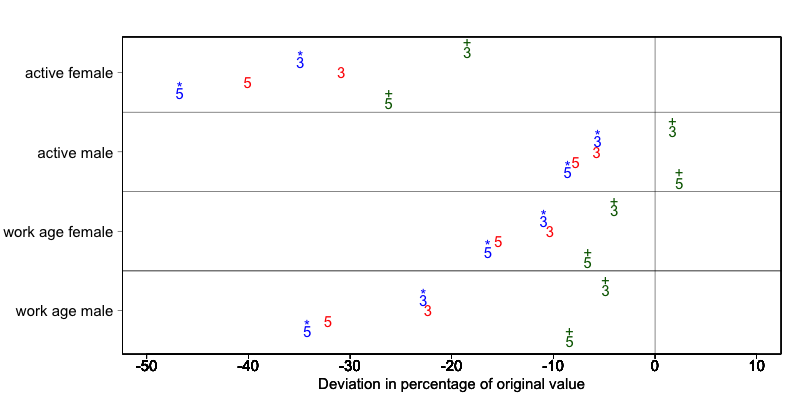
\includegraphics[width=1\linewidth]{Imagenes/image7} \caption{Cambios en los indicadores del mercado laboral tras la anonimización de los datos de I2D2}\label{fig:fig8}
\end{figure}

El umbral de \(k\)-anonimato que debe fijarse depende de varios factores, que son, entre otros:

\begin{enumerate}
\def\labelenumi{\arabic{enumi}.}
\tightlist
\item
  Los requisitos legales para un archivo de datos seguro.
\item
  Otros métodos que se aplicarán a los datos.
\item
  El número de supresiones y la consiguiente pérdida de información resultante de umbrales más altos.
\item
  El tipo de variable.
\item
  Las ponderaciones y el tamaño de la muestra.
\item
  El tipo de publicación (véase la sección \protect\hyperlink{tipos-de-liberaciuxf3n-de-datos}{Tipos de liberación de datos}).
\end{enumerate}

Los niveles aplicados habitualmente para el umbral de \(k\)-anonimato son 3 y 5.

La Tabla \ref{tab:Tabla10} ilustra la influencia del vector de importancia y el umbral de \(k\)-anonimato en el tiempo de ejecución, el riesgo global tras la supresión y el número total de supresiones necesarias para alcanzar este umbral de \(k\)-anonimato. El conjunto de datos contiene unos 63.000 individuos. Cuanto mayor sea el umbral de \(k\)-anonimato, más supresiones serán necesarias y menor será el riesgo tras la supresión local (número esperado de reidentificaciones). En este ejemplo concreto, el tiempo de cálculo es menor para los umbrales más altos. Esto se debe al mayor número de supresiones necesarias, lo que reduce la dificultad de la búsqueda de un patrón de supresión óptimo.

La variable edad se recodifica en intervalos de cinco años y tiene 20 categorías de edad. Esta es la variable con el mayor número de categorías. Dar prioridad a la supresión de otras variables conduce a un mayor número total de supresiones y a un mayor tiempo de cálculo.

\begin{table}

\caption{\label{tab:Tabla10}\label{tab:Tabla10}Efecto de los vectores de importancia y umbrales de $k$-anonimato en el tiempo de ejecución y número total de supresiones}
\centering
\begin{tabular}[t]{clcccc}
\toprule
Umbral k-anonimato & Vector de importancia & Número total de supresiones & Umbral k-anonimato & Vector de importancia & Número total de supresiones\\
\midrule
3 & ninguno   (por defecto) & 6,676 & 5,387 & 293.0 & 11.8\\
3 & situación   laboral & 7,254 & 5,512 & 356.5 & 13.1\\
3 & variable   de edad & 8,175 & 60 & 224.6 & 4.5\\
5 & ninguno   (por defecto) & 9,971 & 7,894 & 164.6 & 8.5\\
5 & situación   laboral & 11,668 & 8,469 & 217.0 & 10.2\\
\addlinespace
5 & variable   de edad & 13,368 & 58 & 123.1 & 3.8\\
\bottomrule
\end{tabular}
\end{table}

En los casos en que hay un gran número de identificadores indirectos y las variables tienen muchas categorías, el número de combinaciones posibles aumenta rápidamente (véase \protect\hyperlink{k-anonimato}{k-anonimato}). Si el número de variables y categorías es muy grande, el tiempo de cálculo del algoritmo \texttt{localSuppression()} puede ser muy largo (véase la sección \protect\hyperlink{tiempo-de-cuxf3mputo}{Tiempo de cómputo} sobre el tiempo de cálculo). Además, es posible que el algoritmo no llegue a una solución, o que llegue a una solución que no cumpla el nivel de \(k\)-anonimato especificado. Por lo tanto, se recomienda reducir el número de identificadores indirectos y/o categorías antes de aplicar la supresión local. Esto puede hacerse recodificando las variables o seleccionando algunas variables para otros métodos (perturbativos), como el PRAM. De este modo se garantiza que el número de supresiones sea limitado y, por tanto, la pérdida de datos se limite solo a los valores que suponen un mayor riesgo.

En algunos conjuntos de datos, puede resultar difícil reducir el número de identificadores indirectos e incluso después de reducir el número de categorías mediante recodificación, el algoritmo de supresión local tarda mucho tiempo en calcular las supresiones necesarias. Una solución en estos casos puede ser el llamado ``enfoque \textbf{all-m}'' (véase \citep{Wolf15}). El enfoque \textbf{all-m} consiste en aplicar el algoritmo de supresión local descrito anteriormente a todos los posibles subconjuntos de tamaño \textbf{m} del conjunto total de identificadores indirectos. La ventaja de este enfoque es que los problemas parciales son más fáciles de resolver y el tiempo de cálculo será menor. Hay que tener cuidado, ya que este método no conduce necesariamente al \(k\)-anonimato en el conjunto completo de identificadores indirectos. Hay dos posibilidades para alcanzar el mismo nivel de protección 1) elegir un umbral más alto para \emph{k} o 2) volver a aplicar el algoritmo de supresión local en el conjunto completo de \emph{k} después de utilizar el método \textbf{all-m} para alcanzar el umbral requerido. En el segundo caso, el enfoque \textbf{all-m} conduce a un menor tiempo de cálculo a costa de un mayor número total de supresiones.

\begin{quote}
\textbf{Nota}: El nivel requerido no se alcanza automáticamente en todo el conjunto de identificadores indirectos si se utiliza el enfoque \textbf{all-m}.
\end{quote}

Por lo tanto, es importante evaluar cuidadosamente las medidas de riesgo después de utilizar el enfoque \textbf{all-m}.

En \texttt{sdcMicro} el enfoque \textbf{all-m} se implementa en el argumento `combs' de la función \texttt{localSuppression()}. El valor de \textbf{m} se especifica en el argumento `combs' y también puede tomar varios valores. Los subconjuntos de diferentes tamaños se utilizan secuencialmente en el algoritmo de supresión local. Por ejemplo, si `combs' se establece como c(3,9), primero se consideran todos los subconjuntos de tamaño 3 y posteriormente todos los subconjuntos de tamaño 9. Establecer el último valor del argumento combs en el número total de variables clave garantiza la consecución del \(k\)-anonimato para el conjunto de datos completo. También es posible especificar diferentes valores de k para cada tamaño de subconjunto en el argumento \emph{k}. Si quisiéramos lograr el anonimato de 5 en los subconjuntos de tamaño 3 y posteriormente el anonimato de 3 en los subconjuntos de tamaño 9, estableceríamos el argumento \emph{k} como c(5,3). El Bloque \ref{exm:bloque22jgm} ilustra el uso del enfoque \textbf{all-m} en \texttt{sdcMicro}.

\begin{example}
\protect\hypertarget{exm:bloque22jgm}{}\label{exm:bloque22jgm}El enfoque \textbf{all-m} en \texttt{sdcMicro}
\end{example}

\begin{Shaded}
\begin{Highlighting}[]
\NormalTok{sdcInitial }\OtherTok{\textless{}{-}} \FunctionTok{undolast}\NormalTok{(sdcInitial)}

\CommentTok{\# Aplicar k{-}anonimato con umbral 5 a todos los subconjuntos de dos variables clave y}
\CommentTok{\# posteriormente al conjunto de datos completo}
\NormalTok{sdcInitial }\OtherTok{\textless{}{-}} \FunctionTok{localSuppression}\NormalTok{(sdcInitial, }\AttributeTok{k =} \DecValTok{5}\NormalTok{, }\AttributeTok{combs =} \FunctionTok{c}\NormalTok{(}\DecValTok{2}\NormalTok{, }\DecValTok{5}\NormalTok{))}
\FunctionTok{print}\NormalTok{(sdcInitial, }\AttributeTok{type=}\StringTok{"ls"}\NormalTok{)}
\end{Highlighting}
\end{Shaded}

\begin{verbatim}
## Local suppression (applied per strata given by variable(s) strata_region)
\end{verbatim}

\begin{verbatim}
##   KeyVar | Suppressions (#) | Suppressions (%)
##  sizeRes |                0 |            0.000
##   AGEYRS |              543 |           27.150
##   GENDER |                0 |            0.000
##   REGION |                0 |            0.000
##    etnia |               63 |            3.150
##    RELIG |               85 |            4.250
\end{verbatim}

\begin{verbatim}
## ----------------------------------------------------------------------
\end{verbatim}

\begin{Shaded}
\begin{Highlighting}[]
\NormalTok{sdcInitial }\OtherTok{\textless{}{-}} \FunctionTok{undolast}\NormalTok{(sdcInitial)}
\CommentTok{\# Aplicar k{-}anonimato con umbral 5 a todos los subconjuntos de tres variables clave y}
\CommentTok{\# posteriormente con el umbral 2 al conjunto de datos completo}
\NormalTok{sdcInitial }\OtherTok{\textless{}{-}} \FunctionTok{localSuppression}\NormalTok{(sdcInitial, }\AttributeTok{k =} \FunctionTok{c}\NormalTok{(}\DecValTok{3}\NormalTok{, }\DecValTok{5}\NormalTok{), }\AttributeTok{combs =} \FunctionTok{c}\NormalTok{(}\DecValTok{5}\NormalTok{, }\DecValTok{2}\NormalTok{))}
\FunctionTok{print}\NormalTok{(sdcInitial, }\AttributeTok{type=}\StringTok{"ls"}\NormalTok{)}
\end{Highlighting}
\end{Shaded}

\begin{verbatim}
## Local suppression (applied per strata given by variable(s) strata_region)
\end{verbatim}

\begin{verbatim}
##   KeyVar | Suppressions (#) | Suppressions (%)
##  sizeRes |                0 |            0.000
##   AGEYRS |              403 |           20.150
##   GENDER |                0 |            0.000
##   REGION |                0 |            0.000
##    etnia |               34 |            1.700
##    RELIG |               42 |            2.100
\end{verbatim}

\begin{verbatim}
## ----------------------------------------------------------------------
\end{verbatim}

La Tabla \ref{tab:Tabla11} presenta los resultados de utilizar el enfoque \textbf{all-m} de un conjunto de datos de prueba con 9 variables clave y 4.000 registros. La Tabla muestra los argumentos \emph{k} y ``combs'' de la función \texttt{localSuppression()}, el número de violaciones de \(k\)-anonimato para diferentes niveles de \emph{k}, así como el número total de supresiones. Observamos que las diferentes combinaciones no siempre conducen al nivel de \(k\)-anonimato requerido. Por ejemplo, cuando se establece \emph{k=3}, y ``combs'' 3 y 7, todavía hay 15 registros en el conjunto de datos (con un total de 9 identificadores indirectos) que violan el anonimato 3 después de la supresión local. Debido al menor tamaño de la muestra, las ganancias en tiempo de ejecución no son todavía evidentes en este ejemplo, ya que la ejecución del algoritmo varias veces consume tiempo. Un conjunto de datos más grande se beneficiaría más del enfoque \textbf{all-m}, ya que el algoritmo tardaría más tiempo.

\begin{table}

\caption{\label{tab:Tabla11}\label{tab:Tabla11}Efecto del enfoque **all-m** en el $k$-anonimato}
\centering
\begin{tabular}[t]{ccccccc}
\toprule
\multicolumn{2}{c}{Argumentos} & \multicolumn{3}{c}{Número de incumplimientos para diferentes niveles de \$k\$-anonimato en el conjunto completo} & \multicolumn{1}{c}{Número total de supresiones} & \multicolumn{1}{c}{Tiempo de ejecución (segundos)} \\
\cmidrule(l{3pt}r{3pt}){1-2} \cmidrule(l{3pt}r{3pt}){3-5} \cmidrule(l{3pt}r{3pt}){6-6} \cmidrule(l{3pt}r{3pt}){7-7}
\multicolumn{1}{c}{k} & \multicolumn{1}{c}{combs} & \multicolumn{1}{c}{k = 2} & \multicolumn{1}{c}{k = 3} & \multicolumn{1}{c}{k = 5} & \multicolumn{1}{c}{.} & \multicolumn{1}{c}{.} \\
\cmidrule(l{3pt}r{3pt}){1-1} \cmidrule(l{3pt}r{3pt}){2-2} \cmidrule(l{3pt}r{3pt}){3-3} \cmidrule(l{3pt}r{3pt}){4-4} \cmidrule(l{3pt}r{3pt}){5-5} \cmidrule(l{3pt}r{3pt}){6-6} \cmidrule(l{3pt}r{3pt}){7-7}
Antes supresión & de la local & 2,464 & 3,324 & 3,877 & 0 & 0.00\\
\midrule
3 & . & 0 & 0 & 1,766 & 2,264 & 17.08\\
5 & . & 0 & 0 & 0 & 3,318 & 10.57\\
3 & 3 & 2,226 & 3,202 & 3,819 & 3,873 & 13.39\\
3 & 3,7 & 15 & 108 & 1,831 & 6,164 & 46.84\\
3 & 3,9 & 0 & 0 & 1,794 & 5,982 & 31.38\\
\addlinespace
3 & 5,9 & 0 & 0 & 1,734 & 6,144 & 62.30\\
5 & 3 & 2,047 & 3,043 & 3,769 & 3,966 & 12.88\\
5 & 3,7 & 0 & 6 & 86 & 7,112 & 46.57\\
5 & 3,9 & 0 & 0 & 0 & 7,049 & 24.13\\
5 & 5,9 & 0 & 0 & 0 & 7,129 & 54.76\\
\addlinespace
5,3 & 3,7 & 11 & 108 & 1,859 & 6,140 & 45.60\\
5,3 & 3,9 & 0 & 0 & 1,766 & 2,264 & 30.07\\
5,3 & 5,9 & 0 & 0 & 0 & 3,318 & 51.25\\
\bottomrule
\end{tabular}
\end{table}

A menudo el conjunto de datos contiene variables relacionadas con las variables clave utilizadas para la supresión local. Ejemplos de ello son las variables rural/urbano a las regiones en caso de que las regiones sean completamente rurales o urbanas o las variables que solo se responden para categorías específicas (por ejemplo, el sector para los que trabajan, las variables relacionadas con la escolaridad para ciertos rangos de edad). En esos casos, las variables rural/urbana o sector podrían no ser identificadores indirectos en sí mismas, pero podrían permitir al intruso reconstruir valores suprimidos en los identificadores indirectos región o situación laboral. Por ejemplo, si la región 1 es completamente urbana y todas las demás regiones son solo semiurbanas o rurales, una supresión en la variable región para un registro de la región 1 puede reconstruirse simplemente mediante la variable rural/urbana. Por lo tanto, es útil suprimir los valores correspondientes a las supresiones en esas variables vinculadas. El Bloque \ref{exm:bloque23jgm} ilustra cómo suprimir los valores de la variable ``urbrur'' correspondientes a las supresiones en la variable región. Todos los valores de ``urbrur'' que corresponden a un valor suprimido \texttt{NA} en la variable ``region'' se suprimen (se ponen a \texttt{NA}).

\begin{example}
\protect\hypertarget{exm:bloque23jgm}{}\label{exm:bloque23jgm}Suprimir manualmente los valores de las variables vinculadas.
\end{example}

\begin{Shaded}
\begin{Highlighting}[]
\CommentTok{\# Suprimir los valores de urbrur en el archivo si la región está suprimida}
\NormalTok{file[}\FunctionTok{is.na}\NormalTok{(sdcInitial}\SpecialCharTok{@}\NormalTok{manipKeyVars}\SpecialCharTok{$}\NormalTok{region) }\SpecialCharTok{\&}
    \SpecialCharTok{!}\FunctionTok{is.na}\NormalTok{(sdcInitial}\SpecialCharTok{@}\NormalTok{origData}\SpecialCharTok{$}\NormalTok{region),}\StringTok{\textquotesingle{}sizRes\textquotesingle{}}\NormalTok{] }\OtherTok{\textless{}{-}} \ConstantTok{NA}
\end{Highlighting}
\end{Shaded}

Como alternativa, las variables vinculadas pueden especificarse al crear el objeto \texttt{sdcMicro}. Las variables vinculadas se denominan variables ``fantasma''. Cualquier supresión en la variable clave conducirá a una supresión en las variables vinculadas a esa variable clave. El Bloque \ref{exm:bloque24jgm} muestra cómo especificar la vinculación entre ``región'' y ``urbrur'' con variables fantasma.

\begin{example}
\protect\hypertarget{exm:bloque24jgm}{}\label{exm:bloque24jgm}Suprimir valores en variables enlazadas especificando variables fantasma
\end{example}

\begin{Shaded}
\begin{Highlighting}[]
\CommentTok{\# Las variables fantasma (vinculadas) se especifican como una lista de vínculos}
\NormalTok{ghostVars }\OtherTok{\textless{}{-}} \FunctionTok{list}\NormalTok{()}

\CommentTok{\# Cada enlace es una lista, con la variable clave en el primer elemento y}
\CommentTok{\# la(s) variable(s) vinculada(s) en el segundo elemento}
\NormalTok{ghostVars[[}\DecValTok{1}\NormalTok{]] }\OtherTok{\textless{}{-}} \FunctionTok{list}\NormalTok{()}
\NormalTok{ghostVars[[}\DecValTok{1}\NormalTok{]][[}\DecValTok{1}\NormalTok{]] }\OtherTok{\textless{}{-}} \StringTok{"REGION"}
\NormalTok{ghostVars[[}\DecValTok{1}\NormalTok{]][[}\DecValTok{2}\NormalTok{]] }\OtherTok{\textless{}{-}} \FunctionTok{c}\NormalTok{(}\StringTok{"URBRUR"}\NormalTok{)}

\CommentTok{\# Crear sdcMicroObj}

\NormalTok{sdcInitial }\OtherTok{\textless{}{-}} \FunctionTok{createSdcObj}\NormalTok{(}\AttributeTok{dat=}\NormalTok{fileHH, }\AttributeTok{keyVars=}\NormalTok{selectedKeyVarsHH, }\AttributeTok{pramVars=}\NormalTok{pramVarsHH, }\AttributeTok{weightVar=}\NormalTok{weightVarHH, }\AttributeTok{numVars =}\NormalTok{ numVarsHH, }\AttributeTok{ghostVars =}\NormalTok{ ghostVars)}

\CommentTok{\# Las variables fantasma manipuladas se encuentran en manipGhostVars}
\FunctionTok{head}\NormalTok{(sdcInitial}\SpecialCharTok{@}\NormalTok{manipGhostVars,}\DecValTok{10}\NormalTok{)}
\end{Highlighting}
\end{Shaded}

\begin{verbatim}
##    URBRUR
## 1       2
## 8       1
## 12      2
## 20      1
## 31      2
## 38      1
## 42      1
## 44      1
## 46      2
## 47      1
\end{verbatim}

La alternativa más sencilla para la función \texttt{localSuppression()} en \texttt{sdcMicro} es la función \texttt{localSupp()}. La función \texttt{localSupp()} puede utilizarse para suprimir los valores de ciertas variables clave de los individuos con riesgos superiores a un determinado umbral. En este caso, se suprimirán todos los valores de la variable especificada para los encuestados con un riesgo superior al umbral especificado. La medida de riesgo utilizada es el riesgo individual (véase la sección \protect\hyperlink{riesgo-individual}{Riesgo individual}. Esto es útil si una variable tiene valores sensibles que no deben publicarse para los individuos con alto riesgo de reidentificación. Lo que se considera alta probabilidad de reidentificación depende de los requisitos legales. En el siguiente ejemplo, los valores de la variable ``educación'' se suprimen para todos los individuos cuyo riesgo individual es superior a 0,08, lo que se ilustra en el Bloque \ref{exm:bloque25jgm}. Para obtener una visión general de los valores de riesgo individuales, puede ser útil observar las estadísticas resumidas de los valores de riesgo individuales, así como el número de supresiones.

\begin{example}
\protect\hypertarget{exm:bloque25jgm}{}\label{exm:bloque25jgm}Aplicación de la función integrada \texttt{sdcMicro} \texttt{localSupp()}
\end{example}

\begin{Shaded}
\begin{Highlighting}[]
\CommentTok{\# Estadísticas resumidas}
\FunctionTok{summary}\NormalTok{(sdcInitial}\SpecialCharTok{@}\NormalTok{risk}\SpecialCharTok{$}\NormalTok{individual[,}\DecValTok{1}\NormalTok{])}
\end{Highlighting}
\end{Shaded}

\begin{verbatim}
##      Min.   1st Qu.    Median      Mean   3rd Qu.      Max. 
## 2.067e-05 7.165e-04 2.847e-03 4.643e-03 5.907e-03 8.541e-02
\end{verbatim}

\begin{Shaded}
\begin{Highlighting}[]
\CommentTok{\# Número de individuos con riesgo individual superior al 0,1}
\FunctionTok{sum}\NormalTok{(sdcInitial}\SpecialCharTok{@}\NormalTok{risk}\SpecialCharTok{$}\NormalTok{individual[,}\DecValTok{1}\NormalTok{] }\SpecialCharTok{\textgreater{}} \FloatTok{0.08}\NormalTok{)}
\end{Highlighting}
\end{Shaded}

\begin{verbatim}
## [1] 2
\end{verbatim}

\begin{Shaded}
\begin{Highlighting}[]
\CommentTok{\# supresión local}
\NormalTok{sdcInitial }\OtherTok{\textless{}{-}} \FunctionTok{localSupp}\NormalTok{(sdcInitial, }\AttributeTok{threshold =} \FloatTok{0.08}\NormalTok{, }\AttributeTok{keyVar =} \StringTok{"etnia"}\NormalTok{)}

\FunctionTok{print}\NormalTok{(sdcInitial, }\AttributeTok{type=}\StringTok{"ls"}\NormalTok{)}
\end{Highlighting}
\end{Shaded}

\begin{verbatim}
## Local suppression:
\end{verbatim}

\begin{verbatim}
##   KeyVar | Suppressions (#) | Suppressions (%)
##  sizeRes |                0 |            0.000
##   AGEYRS |                0 |            0.000
##   GENDER |                0 |            0.000
##   REGION |                0 |            0.000
##    etnia |                2 |            0.100
##    RELIG |                0 |            0.000
\end{verbatim}

\begin{verbatim}
## ----------------------------------------------------------------------
\end{verbatim}

\hypertarget{muxe9todos-perturbativos}{%
\section{Métodos perturbativos}\label{muxe9todos-perturbativos}}

Los métodos perturbativos no suprimen los valores del conjunto de datos, sino que perturban (alteran) los valores para limitar el riesgo de divulgación creando incertidumbre en torno a los valores reales. Un intruso no sabe si una coincidencia entre los microdatos y un archivo externo es correcta o no. La mayoría de los métodos perturbativos se basan en el principio del enmascaramiento matricial, es decir, el conjunto de datos alterado \(Z\) se calcula como

\[Z = AXB + C\]

donde \(X\) son los datos originales, \(A\) es una matriz utilizada para transformar los registros, \(B\) es una matriz para transformar las variables y \(C\) es una matriz con ruido aditivo.

\begin{quote}
\textbf{Nota}: Las medidas de riesgo basadas en el recuento de frecuencias de las claves dejan de ser válidas tras aplicar los métodos perturbativos.
\end{quote}

Esto puede verse en la Tabla \ref{tab:Tabla12}, que muestra los mismos datos antes y después de intercambiar algunos valores. Los valores intercambiados aparecen en cursiva. Tanto antes como después de perturbar los datos, todas las observaciones violan el \(k\)-anonimato en el nivel 3 (es decir, cada clave no aparece más de dos veces en el conjunto de datos). No obstante, el riesgo de reidentificación \textbf{correcta} de los registros se reduce y, por tanto, es posible que no se revele la información contenida en otras variables (sensibles). Con cierta probabilidad, una coincidencia de los microdatos con un archivo de datos externo será errónea. Por ejemplo, un intruso encontraría un individuo con la combinación \{``hombre'', ``urbano'', ``superior''\}, que es una muestra única. Sin embargo, esta coincidencia no es correcta, ya que el conjunto de datos original no contenía ningún individuo con estas características y, por tanto, el individuo coincidente no puede ser una coincidencia correcta. El intruso no puede saber con certeza si la información revelada de otras variables para ese registro es correcta.

\begin{table}

\caption{\label{tab:Tabla12}\label{tab:Tabla12}Efecto del enfoque **all-m** en el $k$-anonimato}
\centering
\begin{tabular}[t]{ccccccc}
\toprule
\multicolumn{1}{c}{Variable} & \multicolumn{3}{c}{Datos originales} & \multicolumn{3}{c}{Después de perturbar los datos} \\
\cmidrule(l{3pt}r{3pt}){1-1} \cmidrule(l{3pt}r{3pt}){2-4} \cmidrule(l{3pt}r{3pt}){5-7}
ID & Sexo & Zona & Educación & Sexo & Zona & Educación\\
\midrule
1 & mujer & rural & superior & mujer & rural & superior\\
2 & mujer & rural & superior & mujer & rural & *media*\\
3 & hombre & rural & media & hombre & rural & media\\
4 & hombre & rural & media & *mujer* & rural & media\\
5 & mujer & urbana & media & *hombre* & urbana & *superior*\\
\addlinespace
6 & mujer & urbana & media & mujer & urbana & media\\
\bottomrule
\end{tabular}
\end{table}

Una de las ventajas de los métodos perturbativos es que se reduce la pérdida de información, ya que no se suprimirán valores, dependiendo del nivel de perturbación. Una desventaja es que los usuarios de los datos pueden tener la impresión de que los datos no se han anonimizado antes de su publicación y estarán menos dispuestos a participar en futuras encuestas. Por lo tanto, es necesario elaborar informes tanto para uso interno como externo (véase \protect\hyperlink{etapa-6.4.5-generar-reportes-y-liberar-datos}{Etapa 6.4.5: Generar reportes y liberar datos}).

Una alternativa a los métodos perturbativos es la generación de archivos de datos sintéticos con las mismas características que los archivos de datos originales. Los archivos de datos sintéticos no se discuten en estas directrices. Aquí abordamos cinco métodos perturbativos: El método de post aleatorización (PRAM), la microagregación, la adición de ruido, el shuffling y el rank swapping.

\hypertarget{pram-muxe9todo-de-post-aleatorizaciuxf3n}{%
\subsection{PRAM (Método de Post-Aleatorización)}\label{pram-muxe9todo-de-post-aleatorizaciuxf3n}}

PRAM es un método perturbativo para datos categóricos. Este método reclasifica los valores de una o más variables, de manera que los intrusos que intentan reidentificar a los individuos en los datos lo hacen, sin embargo, con probabilidad positiva, la reidentificación realizada es con el individuo equivocado. Esto significa que el intruso puede ser capaz de hacer coincidir varios individuos entre los archivos externos y los archivos de datos liberados, pero no puede estar seguro de que estas coincidencias correspondan al individuo correcto.

PRAM se define mediante la matriz de transición \(P\), que especifica las probabilidades de transición, es decir, la probabilidad de que un valor de una determinada variable permanezca inalterado o se cambie a cualquiera de los otros \(k-1\) valores. \(k\) es el número de categorías o niveles del factor dentro de la variable que se va a PRAM. Por ejemplo, si la variable región tiene 10 regiones diferentes, \(k\) es igual a 10. En el caso de PRAM para una sola variable, la matriz de transición es de tamaño \(k∗k\). Ilustramos el PRAM con un ejemplo de la variable ``región'', que tiene tres valores diferentes: ``capital'', ``rural1'' y ``rural2''. La matriz de transición para aplicar PRAM a esta variable es de tamaño 3*3:

\begin{split}
P = 
\begin{bmatrix}
1 & 0 & 0 \\
0.05 & 0.8 & 0.15 \\
0.05 & 0.15 & 0.8 \\
\end{bmatrix}
\end{split}

Los valores de la diagonal son las probabilidades de que un valor de la categoría correspondiente no se modifique. El valor 1 en la posición (1,1) de la matriz significa que todos los valores ``capital'' permanecen ``capital''; esto podría ser una decisión útil, ya que la mayoría de los individuos viven en la capital y no necesitan protección. El valor 0,8 en la posición (2,2) significa que un individuo con valor ``rural1'' se quedará con probabilidad 0,8 ``rural1''. Los valores 0,05 y 0,15 en la segunda fila de la matriz indican que el valor ``rural1'' se cambiará a ``capital'' o ``rural2'' con una probabilidad de 0,05 y 0,15, respectivamente. Si en el fichero inicial teníamos 5.000 individuos con valor ``capital'' y respectivamente 500 y 400 con valores ``rural1'' y ``rural2'', esperamos después de aplicar PRAM tener 5.045 individuos con capital, 460 con rural1 y 395 con rural2 {[}9{]}. La recodificación se realiza de forma independiente para cada individuo. Vemos que la tabulación de la variable ``región'' arroja resultados diferentes antes y después de PRAM, que se muestran en la Tabla \ref{tab:Tabla13}. La desviación de la expectativa se debe a que PRAM es un método probabilístico, es decir, los resultados dependen de un mecanismo de generación de probabilidades; en consecuencia, los resultados pueden diferir cada vez que aplicamos PRAM a las mismas variables de un conjunto de datos.

\begin{quote}
\textbf{Nota}:El número de valores modificados es mayor de lo que podría pensarse al inspeccionar las tabulaciones de la Tabla \ref{tab:Tabla13}. No todos los 5.000 individuos con valor ``capital'' después de PRAM tenían este valor antes de PRAM y los 457 individuos en rural1 después de PRAM no están todos incluidos en los 500 individuos antes de PRAM. El número de cambios es mayor que las diferencias en la tabulación (véase la matriz de transición).
\end{quote}

Dado que la matriz de transición es conocida por los usuarios finales, hay varias formas de corregir el análisis estadístico de los datos por las distorsiones introducidas por el PRAM.

\begin{table}

\caption{\label{tab:Tabla13}\label{tab:Tabla13}Tabulación de la variable "región" antes y después del PRAM}
\centering
\begin{tabular}[t]{ccc}
\toprule
Valor & Tabulación antes de PRAM & Tabulación después de PRAM\\
\midrule
rural1 & 500 & 457\\
rural2 & 400 & 391\\
\bottomrule
\end{tabular}
\end{table}

Una forma de garantizar la consistencia entre las tabulaciones antes y después de PRAM es elegir la matriz de transición de forma que, en la expectativa, las tabulaciones antes y después de aplicar PRAM sean las mismas para todas las variables. {[}10{]} Este método se llama PRAM invariante y se implementa en \texttt{sdcMicro} en la función \texttt{pram()}. El método \texttt{pram()} determina la matriz de transición que satisface los requisitos de PRAM invariante.

\begin{quote}
El PRAM invariante no garantiza que las tabulaciones cruzadas de las variables (a diferencia de las tabulaciones univariantes) permanezcan iguales.
\end{quote}

\begin{Shaded}
\begin{Highlighting}[]
\CommentTok{\# Ejecutamos nuevamente las variables clave}

\NormalTok{selectedKeyVarsHH }\OtherTok{\textless{}{-}} \FunctionTok{c}\NormalTok{(}\StringTok{"URBRUR"}\NormalTok{, }\StringTok{"REGION"}\NormalTok{, }\StringTok{"HHSIZE"}\NormalTok{, }\StringTok{"OWNAGLAND"}\NormalTok{, }\StringTok{"RELIG"}\NormalTok{)}


\NormalTok{HHVars }\OtherTok{\textless{}{-}} \FunctionTok{c}\NormalTok{(}\StringTok{"IDH"}\NormalTok{, selectedKeyVarsHH, pramVarsHH, numVarsHH, weightVarHH, strata\_var) }\CommentTok{\#agrega strata}
\NormalTok{fileHH }\OtherTok{\textless{}{-}}\NormalTok{ file}
\NormalTok{fileHH }\OtherTok{\textless{}{-}}\NormalTok{ fileHH[}\FunctionTok{which}\NormalTok{(}\SpecialCharTok{!}\FunctionTok{duplicated}\NormalTok{(fileHH}\SpecialCharTok{$}\NormalTok{IDH)),]}
\NormalTok{sdcHH }\OtherTok{\textless{}{-}} \FunctionTok{createSdcObj}\NormalTok{(}\AttributeTok{dat=}\NormalTok{fileHH, }\AttributeTok{keyVars=}\NormalTok{selectedKeyVarsHH, }\AttributeTok{pramVars=}\NormalTok{pramVarsHH, }\AttributeTok{weightVar=}\NormalTok{weightVarHH, }\AttributeTok{numVars =}\NormalTok{ numVarsHH, }\AttributeTok{strataVar =} \StringTok{"strata\_region"}\NormalTok{)}

\NormalTok{sdcInitial }\OtherTok{\textless{}{-}}\NormalTok{ sdcHH}
\NormalTok{sdc\_respaldo }\OtherTok{\textless{}{-}}\NormalTok{ sdcHH}
\end{Highlighting}
\end{Shaded}

En el Bloque \ref{exm:bloque26jgm}, damos un ejemplo de PRAM invariante utilizando \texttt{sdcMicro}\footnote{En este ejemplo y en los siguientes de esta sección, el objeto \texttt{sdcMicro} ``sdcIntial'' contiene un conjunto de datos con 2.000 individuos y 39 variables. Seleccionamos cinco identificadores indirectos categóricos y 9 variables para PRAM: ``ROOF'', ``TOILET'', ``WATER'', ``ELECTCON'', ``FUELCOOK'', ``OWNMOTORCYCLE'', ``CAR'', ``TV'' y ``LIVESTOCK''. Estas variabels PRAM se seleccionaron en función de los requisitos de este conjunto de datos concreto y con fines ilustrativos.}. PRAM es un método probabilístico y los resultados pueden diferir cada vez que aplicamos PRAM a las mismas variables de un conjunto de datos. Para superar esto y hacer que los resultados sean reproducibles, es una buena práctica establecer una semilla para el generador de números aleatorios en R, de modo que se generen los mismos números aleatorios cada vez\footnote{El método PRAM en \texttt{sdcMicro} a veces produce el siguiente error: Error in factor(xpramed, labels = lev) : invalid `labels'; length 6 should be 1 or 5. En algunas circunstancias, cambiar la semilla puede resolver este error.}. También, se muestra el número de registros modificados por variable.

\hypertarget{section}{%
\subsubsection{}\label{section}}

\begin{example}
\protect\hypertarget{exm:bloque26jgm}{}\label{exm:bloque26jgm}Producción de resultados reproducibles de PRAM utilizando \texttt{set.seed()}
\end{example}

\begin{Shaded}
\begin{Highlighting}[]
\CommentTok{\# establecer la semilla para la generación de números aleatorios}
\FunctionTok{set.seed}\NormalTok{(}\DecValTok{123}\NormalTok{) }
\NormalTok{sdcInitial\_edit }\OtherTok{\textless{}{-}} \FunctionTok{pram}\NormalTok{(}\AttributeTok{obj =}\NormalTok{ sdcInitial)}

\NormalTok{sdcInitial\_edit}\SpecialCharTok{@}\NormalTok{pram}\SpecialCharTok{$}\NormalTok{summary}
\end{Highlighting}
\end{Shaded}

\begin{verbatim}
##        variable nrChanges percChanges
## 1          ROOF        81        4.05
## 2        TOILET       247       12.35
## 3         WATER       177        8.85
## 4      ELECTCON         7        0.35
## 5      FUELCOOK       160        8.00
## 6 OWNMOTORCYCLE        62        3.10
## 7           CAR        19        0.95
## 8            TV       106        5.30
## 9     LIVESTOCK        23        1.15
\end{verbatim}

La Tabla \ref{tab:Tabla14} muestra la tabulación de la variable después de aplicar el PRAM invariante. Podemos ver que las desviaciones de las tabulaciones iniciales, que tienen expectativa 0, son menores que la matriz de transición que no cumple la propiedad de invariancia. Las desviaciones restantes se deben a la aleatoriedad.

\begin{table}

\caption{\label{tab:Tabla14}\label{tab:Tabla14}Tabulación de la variable "región" antes y después del PRAM (invariante)}
\centering
\begin{tabular}[t]{lccc}
\toprule
Valor & Tabulación antes de PRAM & Tabulación después de PRAM & Tabulación después del PRAM invariante\\
\midrule
capital & 5,000 & 5,052 & 4,998\\
rural1 & 500 & 457 & 499\\
rural2 & 400 & 391 & 403\\
\bottomrule
\end{tabular}
\end{table}

La Tabla \ref{tab:Tabla15} presenta las tabulaciones cruzadas con la variable sexo. Antes de aplicar PRAM invariante, la proporción de hombres en la ciudad es mucho mayor que la de mujeres (alrededor del 60\%). Esta propiedad no se mantiene después de PRAM invariante (los porcentajes de hombres y mujeres en la ciudad son aproximadamente iguales), aunque se mantienen las tabulaciones univariantes. Una solución es aplicar PRAM por separado para los hombres y las mujeres de este ejemplo\footnote{Esto también puede lograrse con matrices de transición multidimensionales. En ese caso, la probabilidad no se especifica para ``masculino'' -\textgreater{} ``feminino'', sino para ``masculino'' + '' rural '' -\textgreater{} ``feminino'' + '' rural '' y para ``masculino'' + ``urbano'' -\textgreater{} ``feminino'' + ``urbano''. Esto no está implementado en \texttt{sdcMicro}, pero se puede lograr mediante PRAMming masculino y feminino por separado. En este ejemplo, esto podría hacerse especificando el género como variable de estrato en la función \texttt{pram()} de \texttt{sdcMicro}.}. Esto puede hacerse especificando el argumento de los estratos en la función \texttt{pram()} de \texttt{sdcMicro} (véase más adelante).

\begin{table}

\caption{\label{tab:Tabla15}\label{tab:Tabla15}Tabulación cruzada de la variable "región" y la variable "sexo" antes y después del PRAM invariante}
\centering
\begin{tabular}[t]{lcccc}
\toprule
\multicolumn{1}{c}{ } & \multicolumn{2}{c}{Tabulación antes de PRAM} & \multicolumn{2}{c}{Tabulación después del PRAM invariante} \\
\cmidrule(l{3pt}r{3pt}){2-3} \cmidrule(l{3pt}r{3pt}){4-5}
Valor & hombre & mujer & hombre & mujer\\
\midrule
capital & 3,056 & 1,944 & 2,623 & 2,375\\
rural1 & 157 & 343 & 225 & 274\\
rural2 & 113 & 287 & 187 & 216\\
\bottomrule
\end{tabular}
\end{table}

La función \texttt{pram()} en \texttt{sdcMicro} tiene varias opciones relacionadas a estratificación (\emph{strata\_variables}), entradas diagonales mínimas para utilizar una matriz de transición P personalizada (\emph{pd}) y la cantidad de perturbación para el método Pram invariante, entregada mediante un vector numérico de longitud 1 (que se reciclará si es necesario) o un vector de la misma longitud que el número de variables.

\begin{quote}
\textbf{Nota}: Si no se establece ninguna opción y el método PRAM se aplica a un objeto \texttt{sdcMicro}, todas las variables PRAM seleccionadas en el objeto \texttt{sdcMicro} se utilizan automáticamente para PRAM y esta se aplica dentro de los estratos seleccionados (véase la sección \protect\hyperlink{objetos-de-la-clase-sdcmicroobj}{Objetos de la clase \texttt{sdcMicroObj}} sobre los objetos \texttt{sdcMicro} para más detalles).
\end{quote}

\hypertarget{section-1}{%
\subsubsection{}\label{section-1}}

\begin{example}
\protect\hypertarget{exm:bloque27jgm}{}\label{exm:bloque27jgm}Selección de variables para aplicar PRAM
\end{example}

\begin{Shaded}
\begin{Highlighting}[]
\FunctionTok{set.seed}\NormalTok{(}\DecValTok{123}\NormalTok{) }\CommentTok{\# establecer la semilla para la generación de números aleatorios}
\CommentTok{\# Aplicar PRAM solo a la variable TOILET}
\NormalTok{sdcInitial }\OtherTok{\textless{}{-}} \FunctionTok{pram}\NormalTok{(}\AttributeTok{obj =}\NormalTok{ sdcInitial, }\AttributeTok{variables =} \FunctionTok{c}\NormalTok{ (}\StringTok{"TOILET"}\NormalTok{))}
\NormalTok{sdcInitial}\SpecialCharTok{@}\NormalTok{pram}\SpecialCharTok{$}\NormalTok{summary}
\end{Highlighting}
\end{Shaded}

\begin{verbatim}
##   variable nrChanges percChanges
## 1   TOILET       106         5.3
\end{verbatim}

Los resultados de PRAM difieren si se aplican simultáneamente a varias variables o posteriormente a cada variable por separado. No es posible especificar toda la matriz de transición en \texttt{sdcMicro}, pero podemos establecer valores mínimos (entre 0 y 1) para las entradas diagonales. Las entradas diagonales especifican la probabilidad de que un determinado valor permanezca igual después de aplicar PRAM. Si fijamos el valor mínimo en 1, no habrá cambios en esta categoría. Por defecto, este valor es 0,8, que se aplica a todas las categorías. También es posible especificar un vector con valor para cada elemento diagonal de la transformación matriz/categoría. En el Bloque \ref{exm:bloque28jgm} los valores de la primera región tienen menos probabilidades de cambiar que los valores de las otras regiones.

\begin{quote}
\textbf{Nota}: El método PRAM invariante requiere que la matriz de transición tenga un valor propio unitario.
\end{quote}

Por lo tanto, no se pueden utilizar todos los conjuntos de restricciones (por ejemplo, el valor mínimo 1 en cualquiera de las categorías).

\hypertarget{section-2}{%
\subsubsection{}\label{section-2}}

\begin{example}
\protect\hypertarget{exm:bloque28jgm}{}\label{exm:bloque28jgm}Especificación de los valores mínimos de la diagonal de la matriz de transición PRAM
\end{example}

\begin{Shaded}
\begin{Highlighting}[]
\NormalTok{sdcInitial }\OtherTok{\textless{}{-}}\NormalTok{ sdc\_respaldo }\CommentTok{\# reasignar}

\NormalTok{sdcInitial }\OtherTok{\textless{}{-}} \FunctionTok{pram}\NormalTok{(}\AttributeTok{obj =}\NormalTok{ sdcInitial, }\AttributeTok{variables =} \FunctionTok{c}\NormalTok{(}\StringTok{"TOILET"}\NormalTok{), }\AttributeTok{pd =} \FunctionTok{c}\NormalTok{(}\FloatTok{0.9}\NormalTok{)) }\CommentTok{\#un valor por variable}

\NormalTok{sdcInitial}\SpecialCharTok{@}\NormalTok{pram}\SpecialCharTok{$}\NormalTok{summary}
\end{Highlighting}
\end{Shaded}

\begin{verbatim}
##   variable nrChanges percChanges
## 1   TOILET       133        6.65
\end{verbatim}

En el método PRAM invariante, también podemos especificar la cantidad de perturbaciones especificando el parámetro alfa. Esta elección se refleja en la matriz de transición. Por defecto, el valor de alfa es 0,5. Cuanto mayor sea alfa, mayores serán las perturbaciones. Un valor de alfa igual a cero no produce cambios. El valor máximo de alfa es 1.

PRAM es especialmente útil cuando un conjunto de datos contiene muchas variables y la aplicación de otros métodos de anonimización, como la recodificación y la supresión local, conduciría a una pérdida significativa de información. Las comprobaciones del riesgo y la utilidad son importantes después de PRAM.

Para hacer inferencia estadística sobre las variables a las que se aplicó PRAM, el investigador necesita conocer el método PRAM, así como la matriz de transición. Sin embargo, la matriz de transición, junto con la semilla de números aleatorios, puede conducir a la divulgación mediante la reconstrucción de los valores no perturbados. Por lo tanto, \textbf{se recomienda publicar la matriz de transición, pero nunca la semilla aleatoria}.

Una desventaja del uso de PRAM es que se pueden generar combinaciones muy improbables, como la de una persona de 63 años que va a la escuela. Por lo tanto, es necesario auditar las variables PRAM para evitar que tales combinaciones se produzcan en el archivo de datos publicado. En principio, la matriz de transición puede diseñarse de forma que ciertas transiciones no sean posibles (probabilidad 0). Por ejemplo, para los que van a la escuela, la edad debe oscilar entre los 6 y los 18 años y solo se permiten esos cambios. En \texttt{sdcMicro} la matriz de transición no puede especificarse exactamente. Una alternativa útil es construir estratos y aplicar PRAM dentro de los estratos. De este modo, los cambios entre variables solo se aplicarán dentro de los estratos. El Bloque \ref{exm:bloque29jgm} ilustra esto aplicando PRAM a la variable ``toilet'' dentro de los estratos generados por la ``region''. Esto evita que se produzcan cambios en la variable ``toilet'', donde se intercambian los tipos de inodoros de una determinada región con los de otras regiones. Por ejemplo, en la región de la capital no se utilizan ciertos tipos de inodoros no mejorados y, por lo tanto, estas combinaciones no deberían producirse después de aplicar PRAM. Los valores solo se cambian con los que están disponibles en el mismo estrato. Los estratos pueden estar formados por cualquier variable categórica, por ejemplo, sexo, grupos de edad, nivel de educación.

\hypertarget{section-3}{%
\subsubsection{}\label{section-3}}

\begin{example}
\protect\hypertarget{exm:bloque29jgm}{}\label{exm:bloque29jgm}Minimizar las combinaciones improbables aplicando el PRAM por estratos
\end{example}

\begin{Shaded}
\begin{Highlighting}[]
\NormalTok{sdcInitial }\OtherTok{\textless{}{-}}\NormalTok{ sdc\_respaldo }\CommentTok{\# reasignar}

\CommentTok{\#Aplicar PRAM dentro de los estratos formados por la variable educ}
\NormalTok{sdcInitial }\OtherTok{\textless{}{-}} \FunctionTok{pram}\NormalTok{(}\AttributeTok{obj =}\NormalTok{ sdcInitial, }\AttributeTok{variables =} \FunctionTok{c}\NormalTok{(}\StringTok{"TOILET"}\NormalTok{), }\AttributeTok{strata\_variables =} \FunctionTok{c}\NormalTok{(}\StringTok{"REGION"}\NormalTok{))}

\NormalTok{sdcInitial}\SpecialCharTok{@}\NormalTok{pram}\SpecialCharTok{$}\NormalTok{summary}
\end{Highlighting}
\end{Shaded}

\begin{verbatim}
##   variable nrChanges percChanges
## 1   TOILET       158         7.9
\end{verbatim}

\begin{quote}
Lectura recomendada de PRAM:
- Gouweleeuw, J. M, P Kooiman, L.C.R.J Willenborg, and P.P de Wolf. ``Post Randomization for Statistical Disclosure Control: Theory and Implementation.'' Journal of Official Statistics 14, no. 4 (1998a): 463-478. Available at \url{http://www.jos.nu/articles/abstract.asp?article=144463}
- Gouweleeuw, J. M, P Kooiman, L.C.R.J Willenborg, and Peter Paul de Wolf. ``The Post Randomization Method for Protecting Microdata.'' Qüestiió, Quaderns d'Estadística i Investigació Operativa 22, no. 1 (1998b): 145-156. Available at \url{http://www.raco.cat/index.php/Questiio/issue/view/2250}
- Marés, Jordi, and Vicenç Torra. 2010.''PRAM Optimization Using an Evolutionary Algorithm.'' In Privacy in Statistical Databases, by Josep Domingo-Ferrer and Emmanouil Magkos, 97-106. Corfú, Greece: Springer.
- Warner, S.L. ``Randomized Response: A Survey Technique for Eliminating Evasive Answer Bias.'' Journal of American Statistical Association 57 (1965): 622-627.
\end{quote}

\hypertarget{microagregaciuxf3n}{%
\subsection{Microagregación}\label{microagregaciuxf3n}}

La microagregación es más adecuada para las variables continuas, pero puede extenderse en algunos casos a las variables categóricas\footnote{La microagregación también se puede utilizar para datos categóricos, siempre que exista la posibilidad de formar grupos y se pueda calcular una sustitución agregada para los valores del grupo. Este es el caso de las variables ordinales.}. Es más útil cuando se han predeterminado reglas de confidencialidad (por ejemplo, se ha establecido un determinado umbral de \(k\)-anonimato) que permiten la divulgación de datos solo si las combinaciones de variables son compartidas por más de un número umbral predeterminado de encuestados (\(k\)). El primer paso en la microagregación es la formación de pequeños grupos de individuos que sean homogéneos con respecto a los valores de las variables seleccionadas, como grupos con ingresos o edad similares. Posteriormente, los valores de las variables seleccionadas de todos los miembros del grupo se sustituyen por un valor común, por ejemplo, la media de ese grupo. Los métodos de microagregación difieren en cuanto a (i) cómo se define la homogeneidad de los grupos, (ii) los algoritmos utilizados para encontrar grupos homogéneos y (iii) la determinación de los valores de sustitución. En la práctica, la microagregación funciona mejor cuando los valores de las variables de los grupos son más homogéneos. En ese caso, la pérdida de información debida a la sustitución de valores por valores comunes para el grupo será menor que en los casos en que los grupos son menos homogéneos.

En el caso univariante, y también para las variables categóricas ordinales, la formación de grupos homogéneos es sencilla: los grupos se forman ordenando primero los valores de la variable y luego creando \(g\) grupos de tamaño \(n_i\) para todos los grupos \(i\) en \(1, ..., g\). Esto maximiza la homogeneidad dentro del grupo, que se mide por la suma al cuadrado de los residuos dentro de los grupos (\(SSE\))

\[
SSE = \sum_{i = 1}^{g}{\sum_{j = 1}^{n_{i}}{\left( x_{ij} - {\overline{x}}_{i} \right)^{T}\left( x_{ij} - {\overline{x}}_{i} \right)}}
\]

Cuanto menor sea \(SSE\), mayor será la homogeneidad dentro del grupo. El tamaño de los grupos puede variar entre ellos, pero a menudo se utilizan grupos de igual tamaño para simplificar la búsqueda\footnote{En este caso, todos los grupos pueden tener diferentes tamaños (es decir, número de individuos en un grupo). En la práctica, la búsqueda de grupos homogéneos se simplifica imponiendo tamaños de grupo iguales para todos los grupos.}.

La función \texttt{microaggregation()} de sdcMicro puede utilizarse para la microagregación univariante. El argumento ``aggr'' especifica el tamaño del grupo. La formación de grupos es más fácil si todos los grupos -excepto quizá el último grupo de los restantes- tienen el mismo tamaño. Este es el caso en la implementación en \texttt{sdcMicro}, ya que no es posible tener grupos de diferentes tamaños. El Bloque \ref{exm:bloque30jgm} muestra cómo utilizar la función \texttt{microaggregation()} en \texttt{sdcMicro}\footnote{En este ejemplo y en los siguientes de esta sección, el objeto \texttt{sdcMicro} ``sdcIntial'' contiene un conjunto de datos con 2.000 individuos y 39 variables. Seleccionamos cinco identificadores indirectos categóricos y tres identificadores indirectos continuos: ``INC'', ``EXP'' y ``WEALTH''.}. El tamaño de grupo por defecto es 3, pero el usuario puede especificar cualquier tamaño de grupo deseado. La elección del tamaño del grupo depende de la homogeneidad dentro de los grupos y del nivel de protección requerido. En general, cuanto más grande sea el grupo, mayor será la protección. Una desventaja de los grupos de igual tamaño es que los datos pueden ser inadecuados para ello. Por ejemplo, si dos individuos tienen un ingreso bajo (por ejemplo, 832 y 966) y cuatro individuos tienen un ingreso alto (por ejemplo, 3.313, 3.211, 2.987, 3.088), la media de dos grupos de tamaño tres (por ejemplo, (832 + 966 + 2.987) / 3 = 1.595 y (3.088 + 3.211 + 3.313) / 3 = 3.204) no representaría ni el ingreso bajo ni el alto.

\hypertarget{section-4}{%
\subsubsection{}\label{section-4}}

\begin{example}
\protect\hypertarget{exm:bloque30jgm}{}\label{exm:bloque30jgm}Aplicación de la microagregación con la función \texttt{sdcMicro} \texttt{microaggregation()}
\end{example}

\begin{Shaded}
\begin{Highlighting}[]
\NormalTok{sdcInitial }\OtherTok{\textless{}{-}}\NormalTok{ sdc\_respaldo }\CommentTok{\# reasignar}

\NormalTok{sdcInitial }\OtherTok{\textless{}{-}} \FunctionTok{microaggregation}\NormalTok{(}\AttributeTok{obj =}\NormalTok{ sdcInitial, }\AttributeTok{variables =} \StringTok{"INCTOTGROSSHH"}\NormalTok{, }\AttributeTok{aggr =} \DecValTok{3}\NormalTok{, }\AttributeTok{method =} \StringTok{"mdav"}\NormalTok{, }\AttributeTok{measure =} \StringTok{"mean"}\NormalTok{)}
\end{Highlighting}
\end{Shaded}

Por defecto, la función de microagregación sustituye los valores por la media del grupo. Un enfoque alternativo y más robusto es reemplazar los valores del grupo con la mediana. Esto puede especificarse en el argumento ``measure'' de la función \texttt{microaggregation()}. En los casos en que se elige la mediana, un individuo de cada grupo mantiene el mismo valor si los grupos tienen tamaños impares. En los casos en los que hay un alto grado de heterogeneidad dentro de los grupos (suele ser el caso de los grupos más grandes), se prefiere la mediana para preservar la información de los datos. Un ejemplo es el ingreso, donde un valor atípico puede dar lugar a múltiples valores atípicos cuando se utiliza la microagregación. Esto se ilustra en la Tabla \ref{tab:Tabla16}. Si elegimos la media como reemplazo de todos los valores, que se agrupan con el valor atípico (6,045 en el grupo 2), a estos registros se les asignarán valores alejados de sus valores originales. Si elegimos la mediana, los ingresos de los individuos 1 y 2 no se ven alterados, pero ningún valor es un valor atípico. Por supuesto, esto puede plantear problemas en sí mismo. En el caso de que la microagregación se aplique a variables categóricas, se utiliza la mediana (el valor en el grupo que más se repite) para calcular el valor de reemplazo de aquel grupo.

\begin{quote}
\textbf{Nota}: Si la microagregación altera los valores atípicos, esto puede tener un impacto significativo en el cálculo de algunas medidas sensibles a los valores atípicos, como el índice GINI.
\end{quote}

\begin{table}

\caption{\label{tab:Tabla16}\label{tab:Tabla16}Ilustración del efecto de la elección de la media frente a la mediana para la microagregación cuando se trata de valores atípicos}
\centering
\begin{tabular}[t]{ccccc}
\toprule
ID & Grupo & Ingresos & Microagregación (media) & Microagregación (mediana)\\
\midrule
1 & 1 & 2,300 & 2,245 & 2,300\\
2 & 2 & 2,434 & 3,608 & 2,434\\
3 & 1 & 2,123 & 2,245 & 2,300\\
4 & 1 & 2,312 & 2,245 & 2,300\\
5 & 2 & 6,045 & 3,608 & 2,434\\
\addlinespace
6 & 2 & 2,345 & 3,608 & 2,434\\
\bottomrule
\end{tabular}
\end{table}

En el caso de múltiples variables candidatas a la microagregación, una posibilidad es aplicar la microagregación univariante a cada una de las variables por separado. La ventaja de la microagregación univariante es la mínima pérdida de información, ya que los cambios en las variables son limitados. Sin embargo, la literatura muestra que el riesgo de divulgación puede ser muy alto si la microagregación univariante se aplica a varias variables por separado y no se aplican técnicas adicionales de anonimización \citep{DMOT02}. Para superar este inconveniente, una alternativa a la microagregación univariante es la microagregación multivariante.

La microagregación multivariada se utiliza ampliamente en las estadísticas oficiales \citep{benschop2019statistical}. El primer paso de la agregación multivariante es la creación de grupos homogéneos basados en varias variables. Los grupos se forman a partir de las distancias multivariadas entre los individuos. Posteriormente, los valores de todas las variables para todos los miembros del grupo se sustituyen por los mismos valores. La Tabla \ref{tab:Tabla17} lo ilustra con tres variables. Vemos que la agrupación por ingresos, gastos y patrimonio conduce a una agrupación diferente, como en el caso de la Tabla \ref{tab:Tabla16}, en la que los grupos se formaron basándose solo en los ingresos.

\begin{table}

\caption{\label{tab:Tabla17}\label{tab:Tabla17}Ilustración de la microagregación multivariante}
\centering
\begin{tabular}[t]{cccccccc}
\toprule
\multicolumn{2}{c}{ } & \multicolumn{3}{c}{Antes de microagregación} & \multicolumn{3}{c}{Después de microagregación} \\
\cmidrule(l{3pt}r{3pt}){3-5} \cmidrule(l{3pt}r{3pt}){6-8}
ID & Grupo & Ingreso & Gasto & Patrimonio & Ingreso & Gasto & Patrimonio\\
\midrule
1 & 1 & 2,300 & 1,714 & 5.3 & 2,285.7 & 1,846.3 & 6.3\\
2 & 1 & 2,434 & 1,947 & 7.4 & 2,285.7 & 1,846.3 & 6.3\\
3 & 1 & 2,123 & 1,878 & 6.3 & 2,285.7 & 1,846.3 & 6.3\\
4 & 2 & 2,312 & 1,950 & 8.0 & 3,567.3 & 2,814.0 & 8.3\\
5 & 2 & 6,045 & 4,569 & 9.2 & 3,567.3 & 2,814.0 & 8.3\\
\addlinespace
6 & 2 & 2,345 & 1,923 & 7.8 & 3,567.3 & 2,814.0 & 8.3\\
\bottomrule
\end{tabular}
\end{table}

Existen varios métodos de microagregación multivariante que difieren en cuanto al algoritmo utilizado para crear grupos de individuos. Además, existe un trade-off entre la velocidad del algoritmo y la homogeneidad dentro del grupo, que está directamente relacionada con la pérdida de información. En el caso de los grandes conjuntos de datos, esto es especialmente difícil. En este artículo se analiza con más detalle el algoritmo de distancia máxima al vector medio (MDAV). El algoritmo MDAV fue introducido por primera vez por \citep{DoTo05} y representa una buena opción con respecto a la compensación entre el tiempo de cálculo y la homogeneidad del grupo, calculada por el \(SSE\) dentro del grupo. El algoritmo MDAV está implementado en \texttt{sdcMicro}.

El algoritmo calcula un registro medio o centroide \(C\), que contiene los valores medios de todas las variables incluidas. Seleccionamos un individuo \(A\) con la mayor distancia euclidiana al cuadrado respecto a \(C\), y construimos un grupo de \(k\) registros alrededor de \(A\). El grupo de \(k\) registros está formado por \(A\) y los \(k-1\) registros más cercanos a \(A\) medidos por la distancia euclidiana. A continuación, seleccionamos otro individuo \(B\), con la mayor distancia euclidiana al cuadrado desde el individuo \(A\). Con los registros restantes, construimos un grupo de \(k\) registros alrededor de \(B\). De la misma manera, seleccionamos un individuo \(D\) con la mayor distancia desde \(B\) y, con los registros restantes, construimos un nuevo grupo de \(k\) registros alrededor de \(D\). El proceso se repite hasta que nos queden menos de \(2∗k\) registros. El algoritmo MDAV crea grupos de igual tamaño con la excepción, quizá, de un último grupo con los remanentes. El conjunto de datos microagregados se calcula sustituyendo cada registro del conjunto de datos original por los valores medios del grupo al que pertenece. Sin embargo, los tamaños de grupo iguales pueden no ser ideales para los datos caracterizados por tener una alta variabilidad. En \texttt{sdcMicro} la microagregación multivariante también se implementa en la función \texttt{microaggregation()}. El Bloque \ref{exm:bloque31jgm} muestra cómo elegir el algoritmo MDAV en \texttt{sdcMicro}.

\hypertarget{section-5}{%
\subsubsection{}\label{section-5}}

\begin{example}
\protect\hypertarget{exm:bloque31jgm}{}\label{exm:bloque31jgm}Microagregación multivariada con el algoritmo de distancia máxima al vector medio (MDAV) en \texttt{sdcMicro}
\end{example}

\begin{Shaded}
\begin{Highlighting}[]
\NormalTok{sdcInitial }\OtherTok{\textless{}{-}} \FunctionTok{createSdcObj}\NormalTok{(}\AttributeTok{dat=}\NormalTok{fileHH, }\AttributeTok{keyVars=}\NormalTok{selectedKeyVarsHH, }\AttributeTok{pramVars=}\NormalTok{pramVarsHH, }\AttributeTok{weightVar=}\NormalTok{weightVarHH, }\AttributeTok{numVars =}\NormalTok{ numVarsHH) }\CommentTok{\# reasignar sin strata var}

\NormalTok{sdcInitial }\OtherTok{\textless{}{-}} \FunctionTok{microaggregation}\NormalTok{(}\AttributeTok{obj =}\NormalTok{ sdcInitial, }\AttributeTok{variables =} \FunctionTok{c}\NormalTok{(}\StringTok{"INCTOTGROSSHH"}\NormalTok{, }\StringTok{"TANHHEXP"}\NormalTok{), }\AttributeTok{method =} \StringTok{"mdav"}\NormalTok{)}

\CommentTok{\#sdc\_respaldo@origData \%\textgreater{}\% view()}
\end{Highlighting}
\end{Shaded}

También es posible agrupar las variables solo dentro de los estratos. Esto reduce el tiempo de cálculo y añade una capa adicional de protección a los datos, debido a la mayor incertidumbre producida \footnote{Además, la homogeneidad en los grupos será generalmente menor, lo que dará lugar a cambios mayores, a una mayor protección, también una mayor pérdida de información, a menos que la variable de estrato esté correlacionada con la variable de microagregación.}. En \texttt{sdcMicro} esto puede lograrse especificando las variables de estrato, como se muestra en el Bloque \ref{exm:bloque32jgm}.

\hypertarget{section-6}{%
\subsubsection{}\label{section-6}}

\begin{example}
\protect\hypertarget{exm:bloque32jgm}{}\label{exm:bloque32jgm}Especificación de variables de estrato para la microagregación
\end{example}

\begin{Shaded}
\begin{Highlighting}[]
\NormalTok{sdcInitial }\OtherTok{\textless{}{-}}\NormalTok{ sdc\_respaldo }\CommentTok{\# reasignar con variable de estrato incluida}

\NormalTok{sdcInitial }\OtherTok{\textless{}{-}} \FunctionTok{microaggregation}\NormalTok{(}\AttributeTok{obj =}\NormalTok{ sdcInitial, }\AttributeTok{variables =} \FunctionTok{c}\NormalTok{(}\StringTok{"INCTOTGROSSHH"}\NormalTok{, }\StringTok{"TANHHEXP"}\NormalTok{), }\AttributeTok{method =} \StringTok{"mdav"}\NormalTok{)}\CommentTok{\#}

\CommentTok{\# No corre el estrato en opción: strata\_variables = c("strata\_region")}
\end{Highlighting}
\end{Shaded}

Además del método MDAV, hay algunos otros métodos de agrupación implementados en \texttt{sdcMicro} \citep{TeMK14}. La Tabla \ref{tab:Tabla18} ofrece un resumen de estos métodos. Mientras que el método ``MDAV'' utiliza la distancia euclidiana, el método ``rmd'' utiliza la distancia de Mahalanobis. Una alternativa a estos métodos es la clasificación de los encuestados basada en el primer componente principal (CP), que es la proyección de todas las variables en un espacio unidimensional que maximiza la varianza de esta proyección. El rendimiento de este método depende de la parte de la varianza total de los datos que explica el primer CP. El método ``rmd'' es más intensivo desde el punto de vista computacional debido al cálculo de las distancias de Mahalanobis, pero proporciona mejores resultados con respecto a la homogeneidad de los grupos. Se recomienda para conjuntos de datos más pequeños \citep{TeMK14}.

\begin{table}

\caption{\label{tab:Tabla18}\label{tab:Tabla18}Métodos de agrupación para la microagregación que son implementados en `sdcMicro`}
\centering
\begin{tabular}[t]{ll}
\toprule
Método / opción en `sdcMicro` & Descripción\\
\midrule
mdav & la agrupación se basa en medidas de distancia clásicas (euclidianas)\\
rmd & la agrupación se basa en medidas de distancia multivariante robusta (Mahalanobis)\\
pca & la agrupación se basa en el análisis de componentes principales, mientras que los datos se clasifican según el primer componente principal\\
clustpppca & la agrupación se basa en el clustering y en el análisis de componentes   principales (robusto) para cada cluster\\
influence & la agrupación se basa en el clustering y la agregación se realiza dentro de los clusters\\
\bottomrule
\end{tabular}
\end{table}

En el caso de que se utilicen múltiples variables para la microagregación, se recomienda examinar primero la matriz de covarianza o de correlación de estas variables. Si no todas las variables están bien correlacionadas, pero dos o más conjuntos de variables muestran una alta correlación, se producirá una menor pérdida de información al aplicar la microagregación por separado a estos conjuntos de variables. En general, si las variables están muy correlacionadas, se producirá una menor pérdida de información al aplicar la microagregación multivariante. La ventaja de sustituir los valores por la media de los grupos en lugar de otros valores de sustitución tiene la ventaja de que se conservan las medias globales de las variables.

\begin{quote}
Lectura recomendada de microagregación:
- Domingo-Ferrer, Josep, and Josep Maria Mateo-Sanz. 2002.''Practical data-oriented microaggregation for statistical disclosure control.'' IEEE Transactions on Knowledge and Data Engineering 14 (2002): 189-201.
- Hansen, Stephen Lee, and Sumitra Mukherjee. 2003. ``A polynomial algorithm for univariate optimal.'' IEEE Transactions on Knowledge and Data Engineering 15 (2003): 1043-1044.
- Hundepool, Anco, Josep Domingo-Ferrer, Luisa Franconi, Sarah Giessing, Rainer Lenz, Jane Naylor, Eric Schulte Nordholt, Giovanni Seri, and Peter Paul de Wolf. 2006. Handbook on Statistical Disclosure Control. ESSNet SDC. \url{http://neon.vb.cbs.nl/casc/handbook.htm}
- Hundepool, Anco, Josep Domingo-Ferrer, Luisa Franconi, Sarah Giessing, Eric Schulte Nordholt, Keith Spicer, and Peter Paul de Wolf. 2012. Statistical Disclosure Control. Chichester: John Wiley \& Sons Ltd.~\url{doi:10.1002/9781118348239}.
- Templ, Matthias, Bernhard Meindl, Alexander Kowarik, and Shuang Chen. 2014, August. ``International Household Survey Network (IHSN).'' \url{http://www.ihsn.org/home/software/disclosure-control-toolbox}. (accessed July 9, 2018).
\end{quote}

\hypertarget{adiciuxf3n-de-ruido}{%
\subsection{Adición de ruido}\label{adiciuxf3n-de-ruido}}

La adición de ruido o enmascaramiento, consiste en añadir o restar valores (pequeños) a los valores originales de una variable, y es lo más adecuado para proteger las variables continuas (véase \citep{Bran02} para una visión general). La adición de ruido puede impedir la coincidencia exacta de las variables continuas. Las ventajas de la adición de ruido son que el ruido es típicamente continuo con media cero, y la coincidencia exacta con archivos externos no será posible. Sin embargo, dependiendo de la magnitud del ruido añadido, la comparación aproximada de intervalos puede ser posible.

Cuando se utiliza la adición de ruido para proteger los datos, es importante tener en cuenta el tipo de datos, el uso previsto de los mismos y las propiedades de los datos antes y después de la adición de ruido, es decir, la distribución -en particular la media-, la covarianza y la correlación entre los conjuntos de datos perturbados y los originales.

Dependiendo de los datos, también puede ser útil comprobar que los valores perturbados están dentro de un rango de valores con sentido. La \ref{fig:fig10} ilustra los cambios en la distribución de los datos con niveles crecientes de ruido. En el caso de los datos que tienen valores atípicos, es importante señalar que cuando la distribución de los datos perturbados es similar a la distribución de los datos originales (por ejemplo, con niveles de ruido bajos), la adición de ruido no protegerá los valores atípicos. Después de la adición de ruido, estos valores atípicos generalmente pueden seguir detectándose como tales y, por tanto, identificarse fácilmente. Un ejemplo es un único valor de ingreso muy elevado en una determinada región. Después de perturbar este valor de ingreso, el valor seguirá siendo reconocido como el ingreso más alto de esa región y, por tanto, puede utilizarse para la reidentificación. Esto se ilustra en la \ref{fig:fig9}, donde se representan 10 observaciones originales (círculos abiertos) y las observaciones anonimizadas (triángulos rojos). La décima observación es un valor atípico. Los valores de las nueve primeras observaciones están suficientemente protegidos por la adición de ruido: su magnitud y orden han cambiado y se puede evitar con éxito la coincidencia exacta o por intervalos. El valor atípico no está suficientemente protegido, ya que, tras la adición de ruido, el valor atípico puede seguir identificándose fácilmente. El hecho de que el valor absoluto haya cambiado no es una protección suficiente. Por otro lado, con niveles de ruido elevados, la protección es mayor incluso para los valores atípicos, pero la estructura de los datos no se conserva y la pérdida de información es grande, lo que no es una situación ideal. Una forma de sortear el problema de los valores atípicos es añadir ruido de mayor magnitud a los valores atípicos que a los demás valores.

\begin{figure}
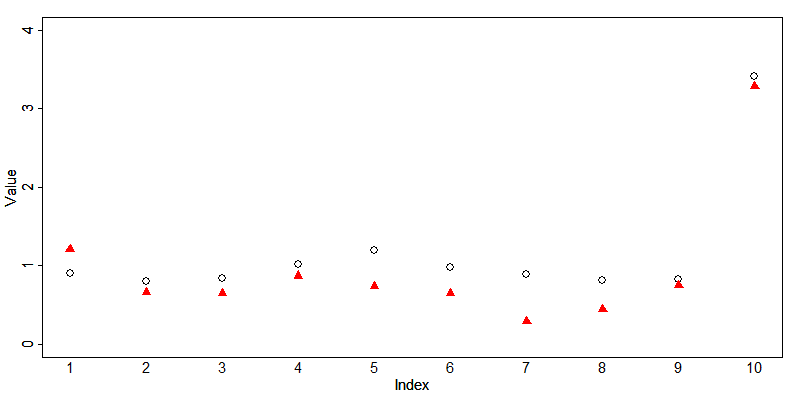
\includegraphics[width=1\linewidth]{Imagenes/image8} \caption{Ilustración del efecto de la adición de ruido a los valores atípicos}\label{fig:fig9}
\end{figure}

Existen varios algoritmos de adición de ruido. La versión más simple de la adición de ruido es el ruido aditivo no correlacionado normalmente distribuido, donde \(x_j\), los valores originales de la variable \(j\) son reemplazados por

\[z_{j} = x_{j} + \varepsilon_{j},\]

donde \(\varepsilon_{j} \sim N(0, \sigma_{\varepsilon_{j}}^{2})\) y \(\sigma_{\varepsilon_{j}} = \alpha * \sigma_{j}\) con \(\sigma_{j}\) la desviación estándar de los datos originales. De este modo, se conservan la media y las covarianzas, pero no las varianzas ni el coeficiente de correlación. Si el nivel de ruido añadido \(\alpha\), se da a conocer al usuario, se pueden estimar muchos estadísticos de forma coherente a partir de los datos perturbados. El ruido añadido es proporcional a la varianza de la variable original. La magnitud del ruido añadido se especifica mediante el parámetro α, que especifica esta proporción. La desviación estándar de los datos perturbados es \(1 + \alpha\) veces la desviación estándar de los datos perturbados. La decisión sobre la magnitud del ruido añadido debe estar informada por la situación legal relativa a la privacidad de los datos, la sensibilidad de los datos y los niveles aceptables de riesgo de divulgación y pérdida de información. En general, el nivel de ruido es una función de la varianza de las variables originales, el nivel de protección necesario y el rango de valores deseado tras la anonimización\footnote{Los valores habituales de \(\alpha\) están entre 0,5 y 2. El valor predeterminado en la función \texttt{addNoise()} de \texttt{sdcMicro} es 150, que es demasiado grande para la mayoría de los conjuntos de datos; el nivel de ruido debe establecerse en el argumento ``noise''.}. Un valor \(\alpha\) demasiado pequeño dará lugar a una protección insuficiente, mientras que un valor \(\alpha\) demasiado alto hará que los datos sean inútiles para los usuarios.

En \texttt{sdcMicro} la adición de ruido se implementa en la función \texttt{addNoise()}. El algoritmo y el parámetro pueden especificarse como argumentos en la función \texttt{addNoise()}. La adición de ruido simple se implementa en la función \texttt{addNoise()} con el valor ``additive'' para el argumento ``method''. El Bloque \ref{exm:bloque33jgm} muestra cómo utilizar \texttt{sdcMicro} para añadir ruido no correlacionado a las variables de gasto, donde la desviación estándar del ruido añadido es igual a la mitad de la desviación estándar de las variables originales\footnote{En este ejemplo y en los siguientes de esta sección, el objeto \texttt{sdcMicro} ``sdcIntial'' contiene un conjunto de datos con 2.000 individuos y 39 variables. Seleccionamos cinco identificadores indirectos categóricos y 12 identificadores indirectos continuos. Se trata de los componentes de gasto ``TFOODEXP'', ``TALCHEXP'', ``TCLTHEXP'', ``THOUSEXP'', ``TFURNEXP'', ``THLTHEXP'', ``TTRANSEXP'', ``TCOMMEXP'', ``TRECEXP'', ``TEDUEXP'', ``TRESTHOTEXP'', ``TMISCEXP''.}. El ruido se añade a todas las variables seleccionadas.

\hypertarget{section-7}{%
\subsubsection{}\label{section-7}}

\begin{example}
\protect\hypertarget{exm:bloque33jgm}{}\label{exm:bloque33jgm}Adición de ruido no correlacionado
\end{example}

\begin{Shaded}
\begin{Highlighting}[]
\NormalTok{sdcInitial }\OtherTok{\textless{}{-}} \FunctionTok{addNoise}\NormalTok{(}\AttributeTok{obj =}\NormalTok{ sdcInitial, }\AttributeTok{variables =} \FunctionTok{c}\NormalTok{(}\StringTok{"TFOODEXP"}\NormalTok{, }\StringTok{"TALCHEXP"}\NormalTok{, }\StringTok{"TCLTHEXP"}\NormalTok{, }\StringTok{"THOUSEXP"}\NormalTok{, }
                                                       \StringTok{"TFURNEXP"}\NormalTok{, }\StringTok{"THLTHEXP"}\NormalTok{, }\StringTok{"TTRANSEXP"}\NormalTok{, }\StringTok{"TCOMMEXP"}\NormalTok{,}
                                                       \StringTok{"TRECEXP"}\NormalTok{, }\StringTok{"TEDUEXP"}\NormalTok{, }\StringTok{"TRESTHOTEXP"}\NormalTok{, }\StringTok{"TMISCEXP"}\NormalTok{), }
                       \AttributeTok{noise =} \FloatTok{0.5}\NormalTok{, }\AttributeTok{method =} \StringTok{"additive"}\NormalTok{)}
\end{Highlighting}
\end{Shaded}

La \ref{fig:fig10} muestra la distribución de frecuencias de una variable numérica continua y la distribución antes y después de la adición de ruido con diferentes niveles de ruido (0.1, 0.5, 1, 2 y 5). El primer gráfico muestra la distribución de los valores originales. Los histogramas muestran claramente que el ruido de grandes magnitudes (valores altos de alfa) conduce a una distribución de los datos alejada de los valores originales. La distribución de los datos pasa a ser una distribución normal cuando la magnitud del ruido crece respectivamente a la varianza de los datos. La media de los datos se conserva, pero, al aumentar el nivel de ruido, la varianza de los datos perturbados crece. Tras añadir un ruido de magnitud 5, la distribución de los datos originales queda completamente alterada.

\begin{figure}
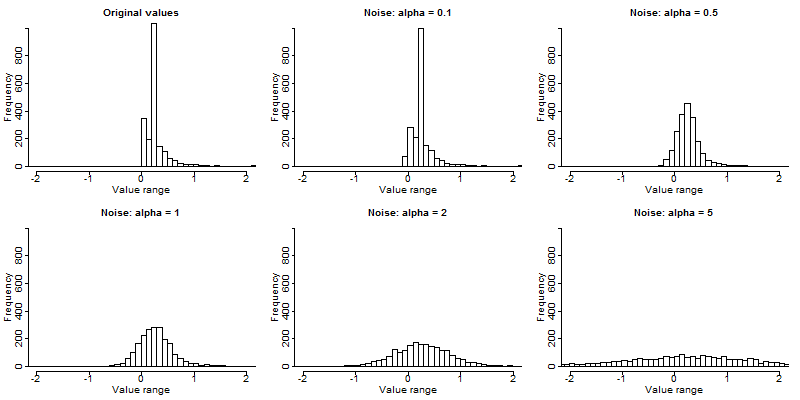
\includegraphics[width=1\linewidth]{Imagenes/image9} \caption{Distribución de frecuencias de una variable continua antes y después de la adición de ruido}\label{fig:fig10}
\end{figure}

La \ref{fig:fig11} muestra el rango de valores de una variable antes de añadir ruido (sin ruido) y después de añadir varios niveles de ruido (α de 0,1 a 1,5 con incrementos de 0,1). En la figura se representan el valor mínimo, los percentiles 20, 30 y 40, la mediana, los percentiles 60, 70, 80 y 90 y el valor máximo. La mediana (percentil 50) se indica con el símbolo rojo ``\(\color {red}{\text{+}}\)''. De las \ref{fig:fig10} y \ref{fig:fig11} se desprende que el rango de valores se amplía tras la adición de ruido, y que la mediana se mantiene aproximadamente en el mismo nivel, al igual que la media por construcción. Cuanto mayor sea la magnitud del ruido añadido, mayor será el rango de valores. En los casos en que la variable debe permanecer en un determinado rango de valores (por ejemplo, solo valores positivos, entre 0 y 100), esto puede ser una desventaja de la adición de ruido. Por ejemplo, las variables de gasto suelen tener valores no negativos, pero la adición de ruido a estas variables puede generar valores negativos, que son difíciles de interpretar. Una forma de evitar este problema es poner a cero los valores negativos. Sin embargo, este truncamiento de los valores por debajo de un determinado umbral distorsionará la distribución (matriz de media y varianza) de los datos perturbados. Esto significa que las características que se preservaron con la adición de ruido, como la conservación de la media y la matriz de covarianza, se pierden y el usuario, incluso con el conocimiento de la magnitud del ruido, ya no puede utilizar los datos para una estimación coherente.

Otra forma de evitar los valores negativos es la aplicación de ruido multiplicativo en lugar de aditivo. En ese caso, las variables se multiplican por un factor aleatorio con esperanza 1 y varianza positiva. Esto también dará lugar a mayores perturbaciones (en valor absoluto) de los valores atípicos. Si la varianza del ruido añadido es pequeña, no habrá factores negativos o serán pocos y, por tanto, habrá menos cambios de signo que en el caso del enmascaramiento por ruido aditivo. El enmascaramiento de ruido multiplicativo no está implementado en \texttt{sdcMicro}, pero puede implementarse con relativa facilidad en \emph{R base} generando un vector de números aleatorios y multiplicando los datos con este vector. Para más información sobre el enmascaramiento de ruido multiplicativo y las propiedades de los datos después del enmascaramiento, nos remitimos a \citep{KiWi03}.

\begin{figure}
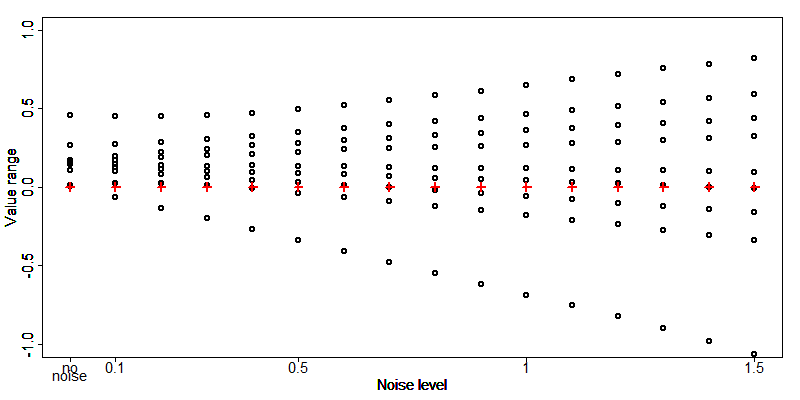
\includegraphics[width=1\linewidth]{Imagenes/image10} \caption{Niveles de ruido y el impacto en el rango de valores (percentiles)}\label{fig:fig11}
\end{figure}

Si se seleccionan dos o más variables para la adición de ruido, se prefiere la adición de ruido correlacionado para preservar la estructura de correlación en los datos. En este caso, la matriz de covarianza del ruido \(\Sigma_{\varepsilon}\) es proporcional a la matriz de covarianza de los datos originales \(\Sigma_{X}\):

\[\Sigma_{\varepsilon} = \alpha \Sigma_{X}\]

En la función \texttt{addNoise()} del paquete sdcMicro, se puede utilizar la adición de ruido correlacionado especificando los métodos ``correlated'' o ``correlated2''. El método ``correlated'' asume que las variables se distribuyen aproximadamente de forma normal. El método ``correlated2'' es una versión del método ``correlated'', que es robusto contra el supuesto de normalidad. El Bloque \ref{exm:bloque34jgm} muestra cómo utilizar el método ``correlated2''. La normalidad de las variables puede investigarse en R, con, por ejemplo, un test Jarque-Bera o Shapiro-Wilk\footnote{La prueba de Shapiro-Wilk se implementa en la función \texttt{shapiro.test()} del paquete \emph{stats} en R. La prueba de Jarque-Bera tiene varias implementaciones en R, por ejemplo, en la función \texttt{jarque.bera.test()} del paquete \emph{tseries}.}.

\hypertarget{section-8}{%
\subsubsection{}\label{section-8}}

\begin{example}
\protect\hypertarget{exm:bloque34jgm}{}\label{exm:bloque34jgm}Adición de ruido correlacionado
\end{example}

\begin{Shaded}
\begin{Highlighting}[]
\NormalTok{sdcInitial }\OtherTok{\textless{}{-}} \FunctionTok{addNoise}\NormalTok{(}\AttributeTok{obj =}\NormalTok{ sdcInitial, }\AttributeTok{variables =} \FunctionTok{c}\NormalTok{(}\StringTok{"TFOODEXP"}\NormalTok{, }\StringTok{"TALCHEXP"}\NormalTok{, }\StringTok{"TCLTHEXP"}\NormalTok{, }\StringTok{"THOUSEXP"}\NormalTok{, }
                                                       \StringTok{"TFURNEXP"}\NormalTok{, }\StringTok{"THLTHEXP"}\NormalTok{, }\StringTok{"TTRANSEXP"}\NormalTok{, }\StringTok{"TCOMMEXP"}\NormalTok{, }
                                                       \StringTok{"TRECEXP"}\NormalTok{, }\StringTok{"TEDUEXP"}\NormalTok{, }\StringTok{"TRESTHOTEXP"}\NormalTok{, }\StringTok{"TMISCEXP"}\NormalTok{), }
                       \AttributeTok{noise =} \FloatTok{0.5}\NormalTok{, }\AttributeTok{method =} \StringTok{"correlated2"}\NormalTok{)}
\end{Highlighting}
\end{Shaded}

En muchos casos, solo hay que proteger los valores atípicos, o hay que protegerlos más. El método ``outdect'' añade ruido solo a los valores atípicos, lo que se ilustra en el Bloque \ref{exm:bloque35jgm}. Los valores atípicos se identifican con métodos univariantes y multivariantes robustos basados en una distancia de Mahalanobis robusta calculada por el estimador MCD \citep{TMKC14}. Sin embargo, la adición de ruido no es el método más adecuado para la protección de los valores atípicos.

\hypertarget{section-9}{%
\subsubsection{}\label{section-9}}

\begin{example}
\protect\hypertarget{exm:bloque35jgm}{}\label{exm:bloque35jgm}Adición de ruido para los valores atípicos mediante el método ``outdect''
\end{example}

\begin{Shaded}
\begin{Highlighting}[]
\NormalTok{sdcInitial }\OtherTok{\textless{}{-}} \FunctionTok{addNoise}\NormalTok{(}\AttributeTok{obj =}\NormalTok{ sdcInitial, }\AttributeTok{variables =} \FunctionTok{c}\NormalTok{(}\StringTok{"TFOODEXP"}\NormalTok{, }\StringTok{"TALCHEXP"}\NormalTok{, }\StringTok{"TCLTHEXP"}\NormalTok{, }\StringTok{"THOUSEXP"}\NormalTok{, }
                                                       \StringTok{"TFURNEXP"}\NormalTok{, }\StringTok{"THLTHEXP"}\NormalTok{, }\StringTok{"TTRANSEXP"}\NormalTok{, }\StringTok{"TCOMMEXP"}\NormalTok{, }
                                                       \StringTok{"TRECEXP"}\NormalTok{, }\StringTok{"TEDUEXP"}\NormalTok{, }\StringTok{"TRESTHOTEXP"}\NormalTok{, }\StringTok{"TMISCEXP"}\NormalTok{), }
                       \AttributeTok{noise =} \FloatTok{0.5}\NormalTok{, }\AttributeTok{method =} \StringTok{"outdect"}\NormalTok{)}
\end{Highlighting}
\end{Shaded}

Si la adición de ruido se aplica a variables que son una proporción de un agregado, esta estructura puede verse seriamente alterada por la adición de ruido. Los ejemplos son los datos de ingresos y gastos con muchas categorías de ingresos y gastos. Las categorías suman el total de ingresos o el total de gastos. En los datos originales, los agregados coinciden con la suma de los componentes. Sin embargo, después de añadir ruido a sus componentes (por ejemplo, diferentes categorías de gasto), sus nuevos agregados ya no coincidirán necesariamente con la suma de las categorías. Una forma de mantener esta estructura es añadir ruido solo a los agregados y liberar los componentes como relación de los agregados perturbados. El Bloque \ref{exm:bloque36jgm} ilustra esto añadiendo ruido al total de los gastos. Posteriormente, se utilizan los cocientes de las categorías de gasto iniciales para cada individuo para reconstruir los valores perturbados de cada categoría de gasto.

\hypertarget{section-10}{%
\subsubsection{}\label{section-10}}

\begin{example}
\protect\hypertarget{exm:bloque36jgm}{}\label{exm:bloque36jgm}Adición de ruido a agregados y sus componentes
\end{example}

\begin{Shaded}
\begin{Highlighting}[]
\CommentTok{\# añadir ruido a los totales (ingresos / gastos)}
\NormalTok{sdcInital }\OtherTok{\textless{}{-}} \FunctionTok{addNoise}\NormalTok{(}\AttributeTok{noise =} \FloatTok{0.5}\NormalTok{, }\AttributeTok{obj =}\NormalTok{ sdcInitial, }\AttributeTok{variables=}\FunctionTok{c}\NormalTok{(}\StringTok{"TANHHEXP"}\NormalTok{, }\StringTok{"INCTOTGROSSHH"}\NormalTok{), }\AttributeTok{method=}\StringTok{"additive"}\NormalTok{) }

\CommentTok{\# multiplicar los totales anonimizados por los ratios para obtener los componentes anonimizados}
\NormalTok{compExp }\OtherTok{\textless{}{-}}  \FunctionTok{c}\NormalTok{(}\StringTok{"TFOODEXP"}\NormalTok{, }\StringTok{"TALCHEXP"}\NormalTok{, }\StringTok{"TCLTHEXP"}\NormalTok{, }\StringTok{"THOUSEXP"}\NormalTok{, }
              \StringTok{"TFURNEXP"}\NormalTok{, }\StringTok{"THLTHEXP"}\NormalTok{, }\StringTok{"TTRANSEXP"}\NormalTok{, }\StringTok{"TCOMMEXP"}\NormalTok{, }
              \StringTok{"TRECEXP"}\NormalTok{, }\StringTok{"TEDUEXP"}\NormalTok{, }\StringTok{"TRESTHOTEXP"}\NormalTok{, }\StringTok{"TMISCEXP"}\NormalTok{)}

\NormalTok{sdcInital}\SpecialCharTok{@}\NormalTok{manipNumVars[,compExp] }\OtherTok{\textless{}{-}}\NormalTok{ sdcInital }\SpecialCharTok{@}\NormalTok{manipNumVars[,}\StringTok{"TANHHEXP"}\NormalTok{] }\SpecialCharTok{*} 
\NormalTok{                                      sdcInital }\SpecialCharTok{@}\NormalTok{origData[,compExp]}\SpecialCharTok{/}\NormalTok{ sdcInital}\SpecialCharTok{@}\NormalTok{origData[,}\StringTok{"TANHHEXP"}\NormalTok{]}

\CommentTok{\# recalcular los riesgos después de cambiar manualmente los valores en el objeto sdcMicro}
\FunctionTok{calcRisks}\NormalTok{(sdcInital)}
\end{Highlighting}
\end{Shaded}

\begin{verbatim}
## The input dataset consists of 2000 rows and 40 variables.
##   --> Categorical key variables: URBRUR, REGION, HHSIZE, OWNAGLAND, RELIG
##   --> Numerical key variables: LANDSIZEHA, TANHHEXP, TFOODEXP, TALCHEXP, TCLTHEXP, THOUSEXP, TFURNEXP, THLTHEXP, TTRANSEXP, TCOMMEXP, TRECEXP, TEDUEXP, TRESTHOTEXP, TMISCEXP, INCTOTGROSSHH, INCRMT, INCWAGE, INCFARMBSN, INCNFARMBSN, INCRENT, INCFIN, INCPENSN, INCOTHER
##   --> Weight variable: WGTPOP
##   --> Strata variable(s): strata_region
## ----------------------------------------------------------------------
\end{verbatim}

\begin{verbatim}
## Information on categorical key variables:
## 
## Reported is the number, mean size and size of the smallest category >0 for recoded variables.
## In parenthesis, the same statistics are shown for the unmodified data.
## Note: NA (missings) are counted as seperate categories!
\end{verbatim}

\begin{verbatim}
##  Key Variable Number of categories      Mean size           
##        URBRUR                    2  (2)  1000.000 (1000.000)
##        REGION                    6  (6)   333.333  (333.333)
##        HHSIZE                   23 (23)    86.957   (86.957)
##     OWNAGLAND                    4  (4)   531.667  (531.667)
##         RELIG                    7  (7)   166.667  (166.667)
##  Size of smallest (>0)      
##                    684 (684)
##                    260 (260)
##                      1   (1)
##                    332 (332)
##                      7   (7)
\end{verbatim}

\begin{verbatim}
## ----------------------------------------------------------------------
\end{verbatim}

\begin{verbatim}
## Infos on 2/3-Anonymity:
## 
## Number of observations violating
##   - 2-anonymity: 115 (5.750%)
##   - 3-anonymity: 239 (11.950%)
##   - 5-anonymity: 497 (24.850%)
## 
## ----------------------------------------------------------------------
\end{verbatim}

\begin{verbatim}
## Numerical key variables: LANDSIZEHA, TANHHEXP, TFOODEXP, TALCHEXP, TCLTHEXP, THOUSEXP, TFURNEXP, THLTHEXP, TTRANSEXP, TCOMMEXP, TRECEXP, TEDUEXP, TRESTHOTEXP, TMISCEXP, INCTOTGROSSHH, INCRMT, INCWAGE, INCFARMBSN, INCNFARMBSN, INCRENT, INCFIN, INCPENSN, INCOTHER
## 
## Disclosure risk is currently between [0.00%; 65.50%]
## 
## Current Information Loss:
##   - IL1: 5502068.37
##   - Difference of Eigenvalues: -3410140045704050.500%
## ----------------------------------------------------------------------
\end{verbatim}

\begin{quote}
Lectura recomendada de adición de ruido:
- Brand, Ruth. 2002. ``Microdata Protection through Noise Addition.'' In Inference -Control in Statistical Databases - From Theory to Practice, edited byJosep Domingo-Ferrer. Lecture Notes in Computer Science Series 2316, 97-116. Berlin Heidelberg: Springer. \url{http://link.springer.com/chapter/10.1007\%2F3-540-47804-3_8}
- Kim, Jay J, and William W Winkler. 2003. ``Multiplicative Noise for Masking Continuous Data.'' Research Report Series (Statistical Research Division. US Bureau of the Census). \url{https://www.census.gov/srd/papers/pdf/rrs2003-01.pdf}
- Torra, Vicenç, and Isaac Cano. 2011. ``Edit Constraints on Microaggregation and Additive Noise.'' In Privacy and Security Issues in Data Mining and Machine Learning, edited by C. Dimitrakakis, A. Gkoulalas-Divanis, A. Mitrokotsa, V. S. Verykios, Y. Saygin. Lecture Notes in Computer Science Volume 6549, 1-14. Berlin Heidelberg: Springer. \url{http://link.springer.com/book/10.1007/978-3-642-19896-0}
- Mivule, K. 2013. ``Utilizing Noise Addition for Data Privacy, An Overview.'' Proceedings of the International Conference on Information and Knowledge Engineering (IKE 2012), (pp.65-71).Las Vegas, USA. \url{http://arxiv.org/ftp/arxiv/papers/1309/1309.3958.pdf}
\end{quote}

\hypertarget{rank-swapping-intercambio-de-rangos}{%
\subsection{Rank swapping (Intercambio de rangos)}\label{rank-swapping-intercambio-de-rangos}}

\emph{Rank swapping} se basa en intercambiar los valores de una determinada variable entre los registros. \emph{Rank swapping} es un tipo de intercambio de datos, que se define para las variables ordinales y continuas. Para \emph{Rank swapping}, los valores de la variable se ordenan primero. El número posible de valores con los que se puede intercambiar una variable está limitado por los valores que se encuentran alrededor del valor original al ordenar los valores del conjunto de datos. El tamaño de este vecindario puede especificarse, por ejemplo, como un porcentaje del número total de observaciones. Esto también significa que un valor puede ser intercambiado con valores iguales o muy similares. Esto es especialmente cierto si la vecindad es pequeña o si solo hay unos pocos valores diferentes en la variable (variable ordinal). Un ejemplo es la variable ``educación'' si tiene pocas categorías: (``ninguna'', ``primaria'', ``secundaria'', ``terciaria''). En estos casos, \emph{Rank swapping} no es un método adecuado al encontrarse con pocas categorías y limitarse por los valores que se encuentran alrededor, para que fuese adecuado, tendría que contar con un número mayor de categorías a intercambiar.

Si \emph{Rank swapping} se aplica a varias variables en simultáneo, la estructura de correlación entre las variables se mantiene. Por lo tanto, es importante comprobar si la estructura de correlación en los datos es plausible. \emph{Rank swapping} se implementa en la función \texttt{rankSwap()} de \texttt{sdcMicro}. Las variables que deben intercambiarse deben especificarse en el argumento ``variables''. Por defecto, los valores por debajo del percentil 5 y por encima del percentil 95 se codifican por arriba y por abajo y se sustituyen por su valor medio (véase la sección \protect\hyperlink{cod-sup-inf}{Codificación superior e inferior}). Especificando las opciones ``TopPercent'' y ``BottomPercent'' podemos elegir estos percentiles. El argumento ``p'' define el tamaño de la vecindad como porcentaje del tamaño de la muestra. Si el valor ``p'' es 0.05, el vecindario tendrá un tamaño de \(0.05 * n\), donde \(n\) es el tamaño de la muestra. Dado que \emph{Rank swapping} es un método probabilístico, es decir, el intercambio depende de un mecanismo generador de números aleatorios, se recomienda especificar una semilla para el generador de números aleatorios antes de utilizar \emph{Rank swapping} y así garantizar la reproducibilidad de los resultados. La semilla también puede especificarse como argumento de la función \texttt{rankSwap()}. El Bloque \ref{exm:bloque37jgm} muestra cómo aplicar \emph{Rank swapping} con \texttt{sdcMicro}. Si las variables contienen valores perdidos (\texttt{NA} en R), la función \texttt{rankSwap()} los recodificará automáticamente con el valor especificado en el argumento ``missing''. Este valor no debe estar en el rango de valores de ninguna de las variables. Después de utilizar la función \texttt{rankSwap()}, estos valores deberían recodificarse como \texttt{NA}. Esto se muestra en el Bloque \ref{exm:bloque37jgm}.

\hypertarget{section-11}{%
\subsubsection{}\label{section-11}}

\begin{example}
\protect\hypertarget{exm:bloque37jgm}{}\label{exm:bloque37jgm}Rank swapping usando \texttt{sdcMicro}
\end{example}

\begin{Shaded}
\begin{Highlighting}[]
\CommentTok{\# establecer la semilla para el generador de números aleatorios }
\FunctionTok{set.seed}\NormalTok{(}\DecValTok{12345}\NormalTok{) }

\CommentTok{\# comprobar la estructura de correlación entre las variables}
\FunctionTok{cor}\NormalTok{(file}\SpecialCharTok{$}\NormalTok{THOUSEXP, file}\SpecialCharTok{$}\NormalTok{TFOODEXP)}
\end{Highlighting}
\end{Shaded}

\begin{verbatim}
## [1] 0.3811335
\end{verbatim}

\begin{Shaded}
\begin{Highlighting}[]
\CommentTok{\# aplicar rank swapping}
\FunctionTok{rankSwap}\NormalTok{(sdcInitial, }\AttributeTok{variables =} \FunctionTok{c}\NormalTok{(}\StringTok{"THOUSEXP"}\NormalTok{, }\StringTok{"TFOODEXP"}\NormalTok{), }\AttributeTok{missing =} \ConstantTok{NA}\NormalTok{) }
\end{Highlighting}
\end{Shaded}

\begin{verbatim}
## setting parameter R0 = 0.95 as no inputs have been specified.
\end{verbatim}

\begin{verbatim}
## The input dataset consists of 2000 rows and 40 variables.
##   --> Categorical key variables: URBRUR, REGION, HHSIZE, OWNAGLAND, RELIG
##   --> Numerical key variables: LANDSIZEHA, TANHHEXP, TFOODEXP, TALCHEXP, TCLTHEXP, THOUSEXP, TFURNEXP, THLTHEXP, TTRANSEXP, TCOMMEXP, TRECEXP, TEDUEXP, TRESTHOTEXP, TMISCEXP, INCTOTGROSSHH, INCRMT, INCWAGE, INCFARMBSN, INCNFARMBSN, INCRENT, INCFIN, INCPENSN, INCOTHER
##   --> Weight variable: WGTPOP
##   --> Strata variable(s): strata_region
## ----------------------------------------------------------------------
\end{verbatim}

\begin{verbatim}
## Information on categorical key variables:
## 
## Reported is the number, mean size and size of the smallest category >0 for recoded variables.
## In parenthesis, the same statistics are shown for the unmodified data.
## Note: NA (missings) are counted as seperate categories!
\end{verbatim}

\begin{verbatim}
##  Key Variable Number of categories      Mean size           
##        URBRUR                    2  (2)  1000.000 (1000.000)
##        REGION                    6  (6)   333.333  (333.333)
##        HHSIZE                   23 (23)    86.957   (86.957)
##     OWNAGLAND                    4  (4)   531.667  (531.667)
##         RELIG                    7  (7)   166.667  (166.667)
##  Size of smallest (>0)      
##                    684 (684)
##                    260 (260)
##                      1   (1)
##                    332 (332)
##                      7   (7)
\end{verbatim}

\begin{verbatim}
## ----------------------------------------------------------------------
\end{verbatim}

\begin{verbatim}
## Infos on 2/3-Anonymity:
## 
## Number of observations violating
##   - 2-anonymity: 115 (5.750%)
##   - 3-anonymity: 239 (11.950%)
##   - 5-anonymity: 497 (24.850%)
## 
## ----------------------------------------------------------------------
\end{verbatim}

\begin{verbatim}
## Numerical key variables: LANDSIZEHA, TANHHEXP, TFOODEXP, TALCHEXP, TCLTHEXP, THOUSEXP, TFURNEXP, THLTHEXP, TTRANSEXP, TCOMMEXP, TRECEXP, TEDUEXP, TRESTHOTEXP, TMISCEXP, INCTOTGROSSHH, INCRMT, INCWAGE, INCFARMBSN, INCNFARMBSN, INCRENT, INCFIN, INCPENSN, INCOTHER
## 
## Disclosure risk is currently between [0.00%; 0.00%]
## 
## Current Information Loss:
##   - IL1: 5536040.91
##   - Difference of Eigenvalues: -5617470445211638.000%
## ----------------------------------------------------------------------
\end{verbatim}

Se ha comprobado que \emph{Rank swapping} da buenos resultados con respecto al equilibrio entre la pérdida de información y la protección de los datos \citep{DoTo01a}. \emph{Rank swapping} no es útil para variables con pocos valores diferentes o muchos valores perdidos, ya que el intercambio en ese caso no dará lugar a valores alterados. Además, si el intruso sabe a quién pertenece el valor más alto o más bajo de una variable específica (por ejemplo, los ingresos), el nivel de esta variable se revelará después de \emph{Rank swapping}, porque los valores en sí no se alteran y los valores originales se revelan todos. Esto puede resolverse codificando por arriba y por abajo los valores más bajos y/o más altos.

\begin{quote}
Lectura recomendada de adición de Rank Swapping:
- Dalenius T. and Reiss S.P. 1978. Data-swapping: a technique for disclosure control (extended abstract). In Proc. ASA Section on Survey Research Methods. American Statistical Association, Washington DC, 191--194.
- Domingo-Ferrer J. and Torra V. 2001. ``A Quantitative Comparison of Disclosure Control Methods for Microdata.'' In Confidentiality, Disclosure and Data Access: Theory and Practical Applications for Statistical Agencies, edited by P. Doyle, J.I. Lane, J.J.M. Theeuwes, and L. Zayatz, 111--134. Amsterdam, North-Holland.
- Hundepool A., Van de Wetering A., Ramaswamy R., Franconi F., Polettini S., Capobianchi A., De Wolf P.-P., Domingo-Ferrer J., Torra V., Brand R. and Giessing S. 2007. μ-Argus User's Manual version 4.1.
\end{quote}

\hypertarget{shuffling-barajado}{%
\subsection{Shuffling (Barajado)}\label{shuffling-barajado}}

El \emph{shuffling} introducido por \citep{MuSa06} es similar al \emph{swapping}, pero utiliza un modelo de regresión subyacente con las variables para determinar cuáles se intercambian. El \emph{shuffling} puede utilizarse para variables continuas y es un método determinista. El \emph{shuffling} mantiene las distribuciones marginales en los datos barajados. Sin embargo, \emph{shuffling} requiere una clasificación completa de los datos, que puede ser muy intensiva desde el punto de vista computacional para grandes conjuntos de datos con múltiples variables.

El método se explica en detalle en \citep{MuSa06}. La idea es clasificar a los individuos en función de sus variables originales. A continuación, se ajusta un modelo de regresión con las variables a proteger como regresores y un conjunto de variables que predicen bien esta variable (es decir, con las que están correlacionadas) como regresores. Este modelo de regresión se utiliza para generar \(n\) valores sintéticos (predichos) para cada variable que hay que proteger. Estos valores generados también se ranquean y cada valor original se sustituye por otro valor original con el rango que corresponde al ranking del valor generado. Esto significa que todos los valores originales estarán en los datos. La Tabla \ref{tab:Tabla19} presenta un ejemplo simplificado del método \emph{shuffling}. En este ejemplo no se especifican los regresores.

\begin{table}

\caption{\label{tab:Tabla19}\label{tab:Tabla19}Métodos de agrupación para la microagregación que son implementados en `sdcMicro`}
\centering
\begin{tabular}[t]{llllll}
\toprule
ID & Ingreso (orig.) & Rango (orig.) & Ingreso (pred.) & Rango (pred.) & Valores barajados\\
\midrule
1 & 2,300 & 2 & 2,466.56 & 4 & 2,345\\
2 & 2,434 & 6 & 2,583.58 & 7 & 2,543\\
3 & 2,123 & 1 & 2,594.17 & 8 & 2,643\\
4 & 2,312 & 3 & 2,530.97 & 6 & 2,434\\
5 & 6,045 & 10 & 5,964.04 & 10 & 6,045\\
\addlinespace
6 & 2,345 & 4 & 2,513.45 & 5 & 2,365\\
7 & 2,543 & 7 & 2,116.16 & 1 & 2,123\\
8 & 2,854 & 9 & 2,624.32 & 9 & 2,854\\
9 & 2,365 & 5 & 2,203.45 & 2 & 2,300\\
10 & 2,643 & 8 & 2,358.29 & 3 & 2,312\\
\bottomrule
\end{tabular}
\end{table}

Se recomienda el uso del método ``ds'' (el método por defecto de \emph{shuffling} en \texttt{sdcMicro}) \citep{TeMK14}. En el argumento ``form'' debe especificarse una función con regresores para las variables a proteger. Al menos dos regresores deben especificarse y estos deben tener poder predictivo para las variables a predecir. Esto puede comprobarse con medidas de bondad de ajuste como el \(R^2\) de la regresión. El \(R^2\) solo capta las relaciones lineales, pero estas son también las únicas relaciones que capta el modelo de regresión lineal utilizado para el \emph{shuffling}. A continuación, se presenta un ejemplo para barajar las variables de gasto, que se predicen mediante el gasto total de los hogares y el tamaño de estos.

\hypertarget{section-12}{%
\subsubsection{}\label{section-12}}

\begin{example}
\protect\hypertarget{exm:bloque38jgm}{}\label{exm:bloque38jgm}Shuffling usando una ecuación de regresión especificada
\end{example}

\begin{Shaded}
\begin{Highlighting}[]
\CommentTok{\# Evaluar el R{-}cuadrado (bondad de ajuste) del modelo de regresión}
\FunctionTok{summary}\NormalTok{(}\FunctionTok{lm}\NormalTok{(file, }\AttributeTok{form =}\NormalTok{ TFOODEXP }\SpecialCharTok{+}\NormalTok{ TALCHEXP }\SpecialCharTok{+}\NormalTok{ TCLTHEXP }\SpecialCharTok{+}\NormalTok{ THOUSEXP }\SpecialCharTok{+}\NormalTok{ TFURNEXP }\SpecialCharTok{+}\NormalTok{ THLTHEXP }\SpecialCharTok{+}\NormalTok{ TTRANSEXP }\SpecialCharTok{+}\NormalTok{ TCOMMEXP }\SpecialCharTok{+}\NormalTok{ TRECEXP }\SpecialCharTok{+}\NormalTok{ TEDUEXP }\SpecialCharTok{+}\NormalTok{ TRESTHOTEXP }\SpecialCharTok{+}\NormalTok{ TMISCEXP }\SpecialCharTok{\textasciitilde{}}\NormalTok{ TANHHEXP }\SpecialCharTok{+}\NormalTok{ HHSIZE)) }
\end{Highlighting}
\end{Shaded}

\begin{verbatim}
## 
## Call:
## lm(formula = TFOODEXP + TALCHEXP + TCLTHEXP + THOUSEXP + TFURNEXP + 
##     THLTHEXP + TTRANSEXP + TCOMMEXP + TRECEXP + TEDUEXP + TRESTHOTEXP + 
##     TMISCEXP ~ TANHHEXP + HHSIZE, data = file)
## 
## Residuals:
##       Min        1Q    Median        3Q       Max 
## -3.92e-10 -5.00e-12 -4.00e-12 -3.00e-12  3.90e-08 
## 
## Coefficients:
##              Estimate Std. Error   t value Pr(>|t|)    
## (Intercept) 2.853e-10  8.003e-12 3.565e+01   <2e-16 ***
## TANHHEXP    1.000e+00  1.075e-16 9.300e+15   <2e-16 ***
## HHSIZE      3.366e-13  1.087e-12 3.100e-01    0.757    
## ---
## Signif. codes:  0 '***' 0.001 '**' 0.01 '*' 0.05 '.' 0.1 ' ' 1
## 
## Residual standard error: 3.794e-10 on 10571 degrees of freedom
## Multiple R-squared:      1,  Adjusted R-squared:      1 
## F-statistic: 4.975e+31 on 2 and 10571 DF,  p-value: < 2.2e-16
\end{verbatim}

\begin{Shaded}
\begin{Highlighting}[]
\CommentTok{\# Shuffling utilizando la ecuación de regresión especificada}
\NormalTok{sdcInitial }\OtherTok{\textless{}{-}} \FunctionTok{shuffle}\NormalTok{(sdcInitial, }\AttributeTok{method=}\StringTok{"ds"}\NormalTok{, }
                      \AttributeTok{form =}\NormalTok{ TFOODEXP }\SpecialCharTok{+}\NormalTok{ TALCHEXP }\SpecialCharTok{+}\NormalTok{ TCLTHEXP }\SpecialCharTok{+}\NormalTok{ THOUSEXP }\SpecialCharTok{+} 
\NormalTok{                        TFURNEXP }\SpecialCharTok{+}\NormalTok{ THLTHEXP }\SpecialCharTok{+}\NormalTok{ TTRANSEXP }\SpecialCharTok{+}\NormalTok{ TCOMMEXP }\SpecialCharTok{+} 
\NormalTok{                        TRECEXP }\SpecialCharTok{+}\NormalTok{ TEDUEXP }\SpecialCharTok{+}\NormalTok{ TRESTHOTEXP }\SpecialCharTok{+}\NormalTok{ TMISCEXP }\SpecialCharTok{\textasciitilde{}}\NormalTok{ TANHHEXP }\SpecialCharTok{+}\NormalTok{ HHSIZE) }
\end{Highlighting}
\end{Shaded}

\begin{quote}
Lectura recomendada de shuffling:
- K. Muralidhar and R. Sarathy. 2006.''Data shuffling - A new masking approach for numerical data,'' Management Science, 52, 658-670.
\end{quote}

\hypertarget{comparaciuxf3n-de-pram-rank-swapping-y-shuffling}{%
\subsection{Comparación de PRAM, Rank swapping y Shuffling}\label{comparaciuxf3n-de-pram-rank-swapping-y-shuffling}}

PRAM, Rank swapping y Shuffling son métodos perturbativos, es decir, cambian los valores de los registros individuales y se utilizan principalmente para las variables continuas. Tras el rank swapping y shuffling, todos los valores originales están contenidos en el conjunto de datos tratado, pero pueden asignarse a otros registros. Esto implica que las tabulaciones univariantes no se modifican. Esto también se mantiene en la expectativa de PRAM, si se elige una matriz de transición que tenga la propiedad invariante.

La elección de un método se basa en la estructura a preservar en los datos. En los casos en los que el modelo de regresión se ajusta a los datos, el shuffling funcionaría muy bien, ya que debería haber suficientes regresores (continuos) disponibles. El rank swapping funciona bien si hay suficientes categorías en las variables. Se prefiere PRAM si el método de perturbación debe aplicarse solo a una o pocas variables; la ventaja es la posibilidad de especificar restricciones en la matriz de transición y aplicar PRAM solo dentro de los estratos, que pueden ser definidos por el usuario.

\hypertarget{anonimizaciuxf3n-del-identificador-indirecto-de-tamauxf1o-del-hogar}{%
\section{Anonimización del identificador indirecto de tamaño del hogar}\label{anonimizaciuxf3n-del-identificador-indirecto-de-tamauxf1o-del-hogar}}

El tamaño de un hogar es un identificador importante, especialmente para los hogares grandes\footnote{En este caso, todos los grupos pueden tener diferentes tamaños (es decir, número de individuos en un grupo). En la práctica, la búsqueda de grupos homogéneos se simplifica teniendo tamaños de grupo iguales para todos los grupos.}. Sin embargo, la supresión de la variable de tamaño real, si está disponible (por ejemplo, el número de miembros del hogar), no basta para eliminar esta información del conjunto de datos, ya que un simple recuento de los miembros del hogar para un hogar concreto permitirá reconstruir esta variable siempre que haya un identificador del hogar en los datos. En cualquier caso, los hogares de un tamaño muy grande o con una clave única o especial (es decir, una combinación de valores de identificadores indirectos) deben comprobarse manualmente. Una forma de tratarlos es eliminar estos hogares del conjunto de datos antes de su publicación. Otra posibilidad es dividir los hogares, pero hay que tener cuidado de suprimir o cambiar los valores de estos hogares para evitar que un intruso entienda inmediatamente que estos hogares han sido divididos y los reconstruya combinando los dos hogares con los mismos valores.

\hypertarget{resumen-de-muxe9todos-sdc}{%
\section{Resumen de métodos SDC}\label{resumen-de-muxe9todos-sdc}}

\begin{table}

\caption{\label{tab:Tablaxx}\label{tab:Tablaxx}Métodos de agrupación para la microagregación que son implementados en `sdcMicro`}
\centering
\begin{tabular}[t]{lllll}
\toprule
Métodos & Técnicas & Ventajas & Desventajas & Tipo de datos\\
\midrule
Perturbativos & PRAM & - Aplicar a subgrupos del conjunto   de datos.
- Probabilidad positiva de un match con un individuo erróneo.
- Seleccionar la matriz de transición y probabilidad.
- Útil con muchas variables y/o alta pérdida de información. & - Modificación de datos originales, se intercambian características.
- Mayor complejidad y posibilidad de error (seleccionar estratos).
- Aparenta que no hay anonimización.
- En el caso de las encuestas por muestreo, cada observación puede tener un   peso muestral diferente, por lo que, después de la generalización, no se garantiza la coherencia. & Categórico\\
Perturbativos & Microagregación & - Sencilla de comprender y aplicar.
- Versión univariada implica baja pérdida de información.
- Versión multivariada permite disminuir bastante el riesgo.
- Todos los valores originales están contenidos en la data tratada   (distribuciones univariadas no cambian).
- Evita la introducción de inconsistencias que requieran edición. & - Trade-off entre pérdida de   información y disminución de riesgo según si se aplica de forma univariado o   multivariada. & Continuo\\
Perturbativos & Adición de ruido & - Puede añadir ruido de forma univariada o bivariada.
- Sencilla de comprender y aplicar. & - Puede mantener niveles altos riesgos, no permite medir los riesgos post-aplicación.
- Variable de número enteros puede pasar a tener decimales (por ejemplo, 3,5   hijos).
- Puede incrementar rango de valores de variable.
- Necesaria edición posterior a la anonimización. & Continuo\\
Perturbativos & Shuffling (Barajado) & - Todos los valores originales están contenidos en la data tratada   (distribuciones univariadas no cambian).
- Permite mantener relaciones multivariadas. & - Requiere una clasificación completa de los datos, que puede ser computacionalmente muy intensiva para grandes conjuntos de datos con varias variables.
- Necesita regresión lineal (deben cumplirse supuestos y la recta ajustar bien)
- La técnica requiere al menos dos variables cuantitativas en la fórmula de   la función. & Continuo\\
Perturbativos & Rank swapping (Intercambio de rangos) & - Todos los valores originales están contenidos en la data tratada (distribuciones univariadas no   cambian).
- Sencilla de comprender y aplicar.
- Permite mantener relaciones multivariadas.
- Baja pérdida de información. & - Reduce rango de valores mínimos y máximos.
- Puede mantener niveles altos de riesgos. & Continuo\\
\addlinespace
No perturbativos & Supresión local & - Quitar datos atípicos.
- Seleccionar datos a eliminar según importancia. & - No es útil para variables continuas ni con alto número de categorías.
- Con alto número de variables o categorías puede no lograr solución.
- Limitación de algoritmo en librería `sdcMicro`.
- Observaciones con variables suprimidas quedan con valor perdido. & Categórico\\
No perturbativos & Recodificación Global & - Se disminuye información, pero   manteniendo estructura y relaciones. & - Pérdida de información continua   al categorizar para estimación de modelos.
- Cambia nivel de medición de variables continuas a ordinales o categóricas. & Continuo y categórico\\
No perturbativos & Codificación superior e inferior & - Se pierde menos información que con recodificación global, permite agrupar solo las colas de la distribución. & - Menor nivel de anonimización, se requiere evaluar trade-off entre ambos métodos. & Continuo y categórico\\
\bottomrule
\end{tabular}
\end{table}

\hypertarget{mediciuxf3n-de-la-utilidad-y-la-puxe9rdida-de-informaciuxf3n}{%
\chapter{Medición de la utilidad y la pérdida de información}\label{mediciuxf3n-de-la-utilidad-y-la-puxe9rdida-de-informaciuxf3n}}

Hoy en día, resolver la tensión entre la protección de la información personal y el suministro de datos es realmente un desafío que deben asumir las ONE. En esta situación, tres motivaciones empujan a las ONE a preservar la confidencialidad.

SDC es un intercambio entre el riesgo de divulgación versus la pérdida de utilidad de los datos (siempre buscando minimizar este último), al tiempo que reduce el riesgo de divulgación a un nivel aceptable. La utilidad de los datos en este contexto significa la utilidad de los datos anonimizados para los análisis estadísticos de los usuarios finales, así como la validez de estos análisis cuando se realizan con datos anonimizados. El riesgo de divulgación y su medición se definirán más adelante en \protect\hyperlink{mediciuxf3n-de-riesgos}{Medición de riesgos}.

Para lograr este equilibrio entre minimizar el riesgo de divulgación y maximizar la utilidad de los datos para los usuarios finales, es necesario medir la utilidad de los datos después de la anonimización y compararla con la utilidad de los datos originales.

En esta sección se busca describir las medidas que se pueden usar para comparar la utilidad de los datos antes y después de la anonimización, así como también cuantificar la pérdida de información. La pérdida de información es inversa a la utilidad de los datos: cuanto mayor sea la utilidad de los datos después de la anonimización, menor será la pérdida de información.

\begin{quote}
\textbf{Nota}
1. Si los microdatos a anonimizar se basan en una muestra, los datos incurrirán en un error de muestreo. También pueden estar presentes otros errores en los datos, como un error de falta de respuesta.
2. Los métodos discutidos aquí solo miden la pérdida de información causada por el proceso de anonimización en relación con los datos de la muestra original y no intentan medir el error causado por otras fuentes.
\end{quote}

La pérdida de información se evalúa con respecto a las necesidades y usos de los usuarios finales de los microdatos. Sin embargo, los diferentes usuarios de los datos anonimizados pueden tener usos muy diversos para los datos publicados y es posible que no sea posible recopilar una lista exhaustiva de los distintos usos. Es así que nos enfocaremos en la publicación de un conjunto de datos para evitar la divulgación no intencional. La publicación de múltiples conjuntos de datos anónimos para diferentes propósitos puede dar lugar a una divulgación no intencionada.\footnote{Es posible liberar archivos de datos para diferentes grupos de usuarios, por ejemplo, PUF y SUF. Sin embargo, toda la información en el archivo menos detallado también debe incluirse en el archivo más detallado para evitar la divulgación no deseada. Los conjuntos de datos publicados en enclaves de datos se pueden personalizar para el usuario, ya que el riesgo de que se combinen con otra versión es cero.}

El proceso SDC se caracteriza por el balance entre el riesgo de divulgación y la utilidad de los datos para los usuarios finales. La escala riesgo-utilidad se extiende entre dos extremos:

\begin{enumerate}
\def\labelenumi{\arabic{enumi}.}
\tightlist
\item
  No se difunden datos (riesgo cero de divulgación) y, por lo tanto, los usuarios no obtienen ninguna utilidad de los datos.
\item
  Los datos se difunden sin ningún tratamiento y, por lo tanto, con el máximo riesgo de divulgación, pero con la máxima utilidad para el usuario (es decir, sin pérdida de información).
\end{enumerate}

El objetivo de un proceso SDC bien implementado es encontrar el punto óptimo en el que la utilidad para los usuarios finales se maximice a un nivel de riesgo aceptable.

En el balance entre Riesgo y Utilidad que se muestra en la Figura @ref(fig:fig1\_sec05), por un extremo, el triángulo corresponde a los datos sin procesar, los que no tienen pérdida de información, pero generalmente tienen un riesgo de divulgación más alto que el nivel aceptable. El otro extremo es el cuadrado, que corresponde a la no publicación de datos. En ese caso, no hay riesgo de divulgación, pero tampoco hay utilidad de los datos para los usuarios. Los puntos intermedios corresponden a diferentes opciones de métodos SDC y/o parámetros aplicados a diferentes variables. El proceso SDC busca
métodos y parámetros, que son aplicados de una manera que produce una reducción del riesgo de forma muchas veces satisfactoria, minimizándose generalmente la pérdida de información.

\begin{figure}

{\centering \includegraphics[width=0.9\linewidth]{Imagenes/fig1} 

}

\caption{Balance riesgo-utilidad en un conjunto de datos.}(\#fig:fig1_sec05)
\end{figure}

\textbf{Fuente:} Imagen extraída de \citep{benschop2021}, pág.78.

En las siguientes secciones, primero proponemos medidas generales de utilidad independientes del uso de datos, y luego presentamos un ejemplo de una medida específica útil para medir la pérdida de información con respecto a usos de datos específicos. Finalmente, mostramos cómo visualizar cambios en los datos causados por la anonimización y discutimos la selección de medidas de utilidad para un conjunto de datos en particular.

\hypertarget{medidas-generales-de-utilidad-para-variables-continuas-y-categuxf3ricas}{%
\section{Medidas generales de utilidad para variables continuas y categóricas}\label{medidas-generales-de-utilidad-para-variables-continuas-y-categuxf3ricas}}

Las medidas generales de pérdida de información se pueden dividir en
aquellas que comparan los valores reales de los datos sin procesar y los
anonimizado, y aquellas que comparan las estadísticas de ambos conjuntos
de datos. Todas las medidas son a posteriori, ya que miden la utilidad
después de la anonimización y requieren tanto los datos originales como
los anonimizados.

Las medidas de utilidad son diferentes para variables categóricas y para
las variables continuas.

\hypertarget{variables-categuxf3ricas}{%
\subsection{Variables categóricas}\label{variables-categuxf3ricas}}

\hypertarget{nuxfamero-de-valores-faltantes}{%
\subsubsection{Número de valores faltantes}\label{nuxfamero-de-valores-faltantes}}

Una medida informativa es comparar el número de valores faltantes en los datos. Los valores faltantes a menudo se producen después de la supresión y a mayor cantidad de aplicación de supresiones será mayor el grado de pérdida de información. Después de usar la función de supresión local en un objeto \texttt{sdcMicro} , la cantidad de supresiones para cada variable clave categórica se puede recuperar con la función print(), como se muestra en el Bloque \ref{exm:bloque1lbn}\footnote{Aquí, el objeto \texttt{sdcMicro} ``sdcIntial'' contiene un conjunto de datos con 2500 personas y 103 variables. Seleccionamos cuatro cuasi-identificadores categóricos: ``URBRUR'', ``REGION'', ``RELIG'' y ``MARITAL'' y varios cuasi-identificadores continuos relativos a ingresos y gastos. Para ilustrar la pérdida de utilidad, también aplicamos varios métodos SDC a este objeto \texttt{sdcMicro} , como supresión local, PRAM y adición de ruido aditivo.}. El argumento `ls' en la función \texttt{print()} es la supresión local. La salida muestra el número absoluto y relativo de supresiones.

\begin{example}
\protect\hypertarget{exm:bloque1lbn}{}\label{exm:bloque1lbn}Uso de la función print() para recuperar el número total de supresiones para cada variable clave categórica
\end{example}

\begin{Shaded}
\begin{Highlighting}[]
\NormalTok{sdcInitial }\OtherTok{\textless{}{-}} \FunctionTok{localSuppression}\NormalTok{(sdcInitial, }\AttributeTok{k =} \DecValTok{5}\NormalTok{, }\AttributeTok{importance =} \ConstantTok{NULL}\NormalTok{)}

\FunctionTok{print}\NormalTok{(sdcInitial, }\StringTok{\textquotesingle{}ls\textquotesingle{}}\NormalTok{)}

\DocumentationTok{\#\# Local Suppression:}
\DocumentationTok{\#\#   KeyVar | Suppressions (\#) | Suppressions (\%)}
\DocumentationTok{\#\#   URBRUR |                0 |            0.000}
\DocumentationTok{\#\#   REGION |               81 |            4.050}
\DocumentationTok{\#\#    RELIG |                0 |            0.000}
\DocumentationTok{\#\#  MARITAL |                0 |            0.000}
\DocumentationTok{\#\# {-}{-}{-}{-}{-}{-}{-}{-}{-}{-}{-}{-}{-}{-}{-}{-}{-}{-}{-}{-}{-}{-}{-}{-}{-}{-}{-}{-}{-}{-}{-}{-}{-}{-}{-}{-}{-}{-}{-}{-}{-}{-}{-}{-}{-}{-}{-}{-}{-}{-}{-}{-}{-}{-}{-}{-}{-}{-}{-}{-}{-}{-}}
\end{Highlighting}
\end{Shaded}

Es posible contar y comparar el número de valores faltantes en los datos originales y los datos tratados. Esto puede ser útil para ver el aumento proporcional en el número de valores faltantes. Los valores faltantes
también pueden tener otras fuentes, como la no respuesta. En el Bloque \ref{exm:bloque2lbn} se muestran los valores faltantes para cada una de las variables clave categóricas en un objeto \texttt{sdcMicro}. Aquí se utiliza el supuesto que todos los valores faltantes están codificados como \texttt{NA}. Si los valores perdidos no están codificados como \texttt{NA}, sino otro valor, se debe utilizar el código de valores perdidos alternativo. Los resultados concuerdan con el número de valores faltantes introducidos por la supresión local en el ejemplo anterior, pero también muestran que la variable ``RELIG'' tiene 1000 valores faltantes en los datos originales.

\begin{example}
\protect\hypertarget{exm:bloque2lbn}{}\label{exm:bloque2lbn}Número de valores faltantes para cada variable clave categórica en un objeto \texttt{sdcMicro}
\end{example}

\begin{Shaded}
\begin{Highlighting}[]
\CommentTok{\# Almacene los nombres de todas las variables clave categóricas en un vector}
\NormalTok{namesKeyVars }\OtherTok{\textless{}{-}} \FunctionTok{names}\NormalTok{(sdcInitial}\SpecialCharTok{@}\NormalTok{manipKeyVars)}

\CommentTok{\# Elaborar una matriz para almacenar el número de valores faltantes (NA) antes y después de la anonimización}
\NormalTok{NAcount }\OtherTok{\textless{}{-}} \FunctionTok{matrix}\NormalTok{(}\ConstantTok{NA}\NormalTok{, }\AttributeTok{nrow =} \DecValTok{2}\NormalTok{, }\AttributeTok{ncol =} \FunctionTok{length}\NormalTok{(namesKeyVars))}
\FunctionTok{colnames}\NormalTok{(NAcount) }\OtherTok{\textless{}{-}} \FunctionTok{c}\NormalTok{(}\FunctionTok{paste0}\NormalTok{(}\StringTok{\textquotesingle{}NA\textquotesingle{}}\NormalTok{, namesKeyVars)) }\CommentTok{\# column names}
\FunctionTok{rownames}\NormalTok{(NAcount) }\OtherTok{\textless{}{-}} \FunctionTok{c}\NormalTok{(}\StringTok{\textquotesingle{}initial\textquotesingle{}}\NormalTok{, }\StringTok{\textquotesingle{}treated\textquotesingle{}}\NormalTok{) }\CommentTok{\# row names}

\CommentTok{\# Recuento de NA en todas las variables clave (NOTA: solo se cuentan las codificadas como NA)}
\ControlFlowTok{for}\NormalTok{(i }\ControlFlowTok{in} \DecValTok{1}\SpecialCharTok{:}\FunctionTok{length}\NormalTok{(namesKeyVars)) \{}
\NormalTok{  NAcount[}\DecValTok{1}\NormalTok{, i] }\OtherTok{\textless{}{-}} \FunctionTok{sum}\NormalTok{(}\FunctionTok{is.na}\NormalTok{(sdcInitial}\SpecialCharTok{@}\NormalTok{origData[,namesKeyVars[i]]))}
\NormalTok{  NAcount[}\DecValTok{2}\NormalTok{, i] }\OtherTok{\textless{}{-}} \FunctionTok{sum}\NormalTok{(}\FunctionTok{is.na}\NormalTok{(sdcInitial}\SpecialCharTok{@}\NormalTok{manipKeyVars[,i]))}
\NormalTok{\}}

\CommentTok{\# Mostrar resultados}
\NormalTok{NAcount}
\DocumentationTok{\#\# NAURBRUR NAREGION NARELIG NAMARITAL}
\DocumentationTok{\#\# inicial 0 0 1000 51}
\DocumentationTok{\#\# tratado 0 81 1000 51}
\end{Highlighting}
\end{Shaded}

\hypertarget{nuxfamero-de-registros-cambiados}{%
\subsubsection{Número de registros cambiados}\label{nuxfamero-de-registros-cambiados}}

Otra estadística útil es el número de registros modificados por variable. Estos se pueden contabilizar de forma similar a los valores perdidos e incluyen supresiones (es decir, cambios en los valores perdidos/\texttt{NA} en \texttt{R} ). El número de registros cambiados es un buen indicador del impacto de los métodos de anonimización en los datos. A
continuación en el Bloque \ref{exm:bloque3lbn} se muestra cómo calcular la cantidad de registros modificados para las variables PRAMmed.

\begin{example}
\protect\hypertarget{exm:bloque3lbn}{}\label{exm:bloque3lbn}Cálculo del número de registros modificados por variable
\end{example}

\begin{Shaded}
\begin{Highlighting}[]
\CommentTok{\# Almacene los nombres de todas las variables del pram en un vector}
\NormalTok{namesPramVars }\OtherTok{\textless{}{-}} \FunctionTok{names}\NormalTok{(sdcInitial}\SpecialCharTok{@}\NormalTok{manipPramVars)}

\CommentTok{\# Marco para guardar la cantidad de registros modificados}
\NormalTok{recChanged }\OtherTok{\textless{}{-}} \FunctionTok{rep}\NormalTok{(}\DecValTok{0}\NormalTok{, }\FunctionTok{length}\NormalTok{(namesPramVars))}
\FunctionTok{names}\NormalTok{(recChanged) }\OtherTok{\textless{}{-}} \FunctionTok{c}\NormalTok{(}\FunctionTok{paste0}\NormalTok{(}\StringTok{\textquotesingle{}RC\textquotesingle{}}\NormalTok{, namesPramVars))}

\CommentTok{\# Cuenta del número de registros cambiados}
\ControlFlowTok{for}\NormalTok{(j }\ControlFlowTok{in} \DecValTok{1}\SpecialCharTok{:}\FunctionTok{length}\NormalTok{(namesPramVars)) }\CommentTok{\# para todas las  variables clave}
\NormalTok{\{}
\NormalTok{  comp }\OtherTok{\textless{}{-}}\NormalTok{ sdcInitial}\SpecialCharTok{@}\NormalTok{origData[namesPramVars[j]] }\SpecialCharTok{!=}
\NormalTok{                              sdcInitial}\SpecialCharTok{@}\NormalTok{manipPramVars[namesPramVars[j]]}
\NormalTok{  temp1 }\OtherTok{\textless{}{-}} \FunctionTok{sum}\NormalTok{(comp, }\AttributeTok{na.rm =} \ConstantTok{TRUE}\NormalTok{) }\CommentTok{\# cambio en todas las variables sin NA}
\NormalTok{  temp2 }\OtherTok{\textless{}{-}} \FunctionTok{sum}\NormalTok{(}\FunctionTok{is.na}\NormalTok{(comp))        }\CommentTok{\# contabiliza los NA en el vector}
\NormalTok{  temp3 }\OtherTok{\textless{}{-}} \FunctionTok{sum}\NormalTok{(}\FunctionTok{is.na}\NormalTok{(sdcInitial}\SpecialCharTok{@}\NormalTok{origData[namesPramVars[j]])}
               \SpecialCharTok{+} \FunctionTok{is.na}\NormalTok{(sdcInitial}\SpecialCharTok{@}\NormalTok{manipPramVars[namesPramVars[j]])}\SpecialCharTok{==}\DecValTok{2}\NormalTok{)}
  \CommentTok{\# ambos NA, sin cambios, contabilizados en temp2}
\NormalTok{  recChanged[j] }\OtherTok{\textless{}{-}}\NormalTok{ temp1 }\SpecialCharTok{+}\NormalTok{ temp2 }\SpecialCharTok{{-}}\NormalTok{ temp3}
\NormalTok{\}}

\CommentTok{\# Mostrar resultados}
\NormalTok{recChanged}
\DocumentationTok{\#\#  RCWATER   RCROOF RCTOILET}
\DocumentationTok{\#\#      125       86      180}
\end{Highlighting}
\end{Shaded}

\hypertarget{comparaciuxf3n-de-tablas-de-contingencia}{%
\subsubsection{Comparación de tablas de contingencia}\label{comparaciuxf3n-de-tablas-de-contingencia}}

Una forma útil de medir la pérdida de información en variables categóricas es comparar tabulaciones univariadas y, lo que es más interesante, tablas de contingencia (también tabulaciones cruzadas o tablas de doble entrada) entre pares de variables. Para mantener la validez analítica de un conjunto de datos, las tablas de contingencia
deben permanecer aproximadamente iguales. La función \texttt{table()} produce tablas de contingencia de una o más variables. El Bloque \ref{exm:bloque4lbn} a continuación crea una tabla de contingencia de las variables ``REGION'' y ``URBRUR''. Observamos pequeñas diferencias entre las tablas antes y después de la anonimización.

\begin{example}
\protect\hypertarget{exm:bloque4lbn}{}\label{exm:bloque4lbn}Comparación de tablas de contingencia de variables categóricas
\end{example}

\begin{Shaded}
\begin{Highlighting}[]
\CommentTok{\# Tabla de contingencia (tabulación cruzada) de las variables region y urban/rural}
 \FunctionTok{table}\NormalTok{(sdcInitial}\SpecialCharTok{@}\NormalTok{origData[, }\FunctionTok{c}\NormalTok{(}\StringTok{\textquotesingle{}REGION\textquotesingle{}}\NormalTok{, }\StringTok{\textquotesingle{}URBRUR\textquotesingle{}}\NormalTok{)]) }\CommentTok{\# antes de la anonimización}
 \DocumentationTok{\#\#       URBRUR}
 \DocumentationTok{\#\# REGION   1   2}
 \DocumentationTok{\#\#      1 235  89}
 \DocumentationTok{\#\#      2 261  73}
 \DocumentationTok{\#\#      3 295  76}
 \DocumentationTok{\#\#      4 304  71}
 \DocumentationTok{\#\#      5 121 139}
 \DocumentationTok{\#\#      6 100 236}

 \FunctionTok{table}\NormalTok{(sdcInitial}\SpecialCharTok{@}\NormalTok{manipKeyVars[, }\FunctionTok{c}\NormalTok{(}\StringTok{\textquotesingle{}REGION\textquotesingle{}}\NormalTok{, }\StringTok{\textquotesingle{}URBRUR\textquotesingle{}}\NormalTok{)]) }\CommentTok{\# después de la anonimización}
 \DocumentationTok{\#\#       URBRUR}
 \DocumentationTok{\#\# REGION   1   2}
 \DocumentationTok{\#\#      1 235  89}
 \DocumentationTok{\#\#      2 261  73}
 \DocumentationTok{\#\#      3 295  76}
 \DocumentationTok{\#\#      4 304  71}
 \DocumentationTok{\#\#      5 105 130}
 \DocumentationTok{\#\#      6  79 201}
\end{Highlighting}
\end{Shaded}

\citep{domingo-ferrer2001}proponen una medida de pérdida de información basada en tablas de contingencia, que cuantifica la distancia entre las tablas de contingencia en los datos originales y los tratados.
Alternativamente, se pueden usar visualizaciones de la tabla de contingencia con gráficos de mosaico para comparar el impacto de los métodos de anonimización en las tabulaciones y tablas de contingencia (consulte la \protect\hyperlink{gruxe1ficos-de-mosaico}{Gráficos de mosaico}).

\hypertarget{variables-continuas}{%
\subsection{Variables continuas}\label{variables-continuas}}

\hypertarget{estaduxedsticas-media-covarianza-correlaciuxf3n}{%
\subsubsection{Estadísticas: media, covarianza, correlación}\label{estaduxedsticas-media-covarianza-correlaciuxf3n}}

Las estadísticas que caracterizan el conjunto de datos no deben cambiar después de la anonimización, como lo son la media, varianza, covarianza y la correlación entre las variables más importantes en el conjunto de
datos. \citep{domingo-ferrer2001} da una visión general de las estadísticas que se pueden considerar. Para evaluar la pérdida de información causada por la anonimización, se deben comparar las estadísticas apropiadas para las variables continuas antes y después de la anonimización.

Para evaluar la pérdida de utilidad se cuentan con varias formas de cálculo, por ejemplo, comparando medias y (co-)varianzas en los datos o comparando las distribuciones (multivariadas) de los datos. Especialmente los cambios en las correlaciones brindan información valiosa sobre la validez de los datos para las regresiones. Las
funciones del paquete base \texttt{R} o cualquier otro paquete estadístico se pueden usar para hacer esto. Los siguientes son algunos ejemplos en \texttt{R}.

Para calcular la media de cada variable numérica usamos la función \texttt{colMeans()}. Para ignorar los valores perdidos, es necesario utilizar la opción \texttt{na.rm\ =\ TRUE}. ``numVars'' es un vector con los nombres de las variables numéricas. El Bloque \ref{exm:bloque5lbn} muestra cómo calcular las medias de todas las variables numéricas. Los datos no tratados se extraen de la ranura `origData' del objeto \texttt{sdcMicro} y los datos anonimizados del \emph{slot} `manipNumVars', que contiene las variables numéricas manipuladas. Observamos pequeños cambios en cada una de las tres variables.

\begin{example}
\protect\hypertarget{exm:bloque5lbn}{}\label{exm:bloque5lbn}Comparando las medias de variables continuas
\end{example}

\begin{Shaded}
\begin{Highlighting}[]
\CommentTok{\# datos no tratados}
\FunctionTok{colMeans}\NormalTok{(sdcInitial}\SpecialCharTok{@}\NormalTok{origData[, numVars], }\AttributeTok{na.rm =} \ConstantTok{TRUE}\NormalTok{)}
\DocumentationTok{\#\#       INC    INCRMT   INCWAGE}
\DocumentationTok{\#\#  479.7710  961.0295 1158.1330}

\CommentTok{\# datos anonimizados}
\FunctionTok{colMeans}\NormalTok{(sdcInitial}\SpecialCharTok{@}\NormalTok{manipNumVars[, numVars], }\AttributeTok{na.rm =} \ConstantTok{TRUE}\NormalTok{)}
\DocumentationTok{\#\#       INC    INCRMT   INCWAGE}
\DocumentationTok{\#\#  489.6030  993.8512 1168.7561}
\end{Highlighting}
\end{Shaded}

De la misma manera, se pueden calcular las matrices de correlación y covarianza de las variables numéricas en el objeto \emph{sdcMicro} a partir de los datos no tratados y anonimizados. Esto se muestra en el Bloque \ref{exm:bloque6lbn}. Observamos que la varianza de cada variable (los elementos diagonales en la matriz de covarianza) ha aumentado por la anonimización. Estas funciones también permiten calcular intervalos de confianza en el caso de muestras. Las medias y las covarianzas de los subconjuntos de los datos tampoco deberían diferir. Un ejemplo es la media de ingresos por género, por grupo de edad o por región. Este tipo de características de los datos son importantes para el análisis.

\begin{example}
\protect\hypertarget{exm:bloque6lbn}{}\label{exm:bloque6lbn}Comparación de estructuras de covarianza y matrices de correlación de variables numéricas
\end{example}

\begin{Shaded}
\begin{Highlighting}[]
\CommentTok{\# datos no tratados}
\FunctionTok{cov}\NormalTok{(sdcInitial}\SpecialCharTok{@}\NormalTok{origData[, numVars])}
\DocumentationTok{\#\#               INC    INCRMT  INCWAGE}
\DocumentationTok{\#\# INC     1645926.1  586975.6  2378901}
\DocumentationTok{\#\# INCRMT   586975.6 6984502.3  1664257}
\DocumentationTok{\#\# INCWAGE 2378900.7 1664257.4 16169878}

\FunctionTok{cor}\NormalTok{(sdcInitial}\SpecialCharTok{@}\NormalTok{origData[, numVars])}

\DocumentationTok{\#\#               INC    INCRMT   INCWAGE}
\DocumentationTok{\#\# INC     1.0000000 0.1731200 0.4611241}
\DocumentationTok{\#\# INCRMT  0.1731200 1.0000000 0.1566028}
\DocumentationTok{\#\# INCWAGE 0.4611241 0.1566028 1.0000000}

\CommentTok{\# datos anonimizados}
\FunctionTok{cov}\NormalTok{(sdcInitial}\SpecialCharTok{@}\NormalTok{manipNumVars[, numVars])}
\DocumentationTok{\#\#               INC    INCRMT  INCWAGE}
\DocumentationTok{\#\# INC     2063013.1  649937.5  2382447}
\DocumentationTok{\#\# INCRMT   649937.5 8566169.1  1778985}
\DocumentationTok{\#\# INCWAGE 2382447.4 1778985.1 19925870}

\FunctionTok{cor}\NormalTok{(sdcInitial}\SpecialCharTok{@}\NormalTok{manipNumVars[, numVars])}
\DocumentationTok{\#\#               INC    INCRMT   INCWAGE}
\DocumentationTok{\#\# INC     1.0000000 0.1546063 0.3715897}
\DocumentationTok{\#\# INCRMT  0.1546063 1.0000000 0.1361665}
\DocumentationTok{\#\# INCWAGE 0.3715897 0.1361665 1.0000000}
\end{Highlighting}
\end{Shaded}

\citep{domingo-ferrer2001} propone varias medidas para la diferencia entre las matrices de covarianza y las de correlación. Estas medidas se basan en el error cuadrático medio, el error absoluto medio o la variación media de las celdas individuales. Nos referimos a \citep{domingo-ferrer2001} para obtener una descripción completa de estas medidas.

\hypertarget{medida-de-puxe9rdida-de-informaciuxf3n-il1s}{%
\subsubsection{Medida de pérdida de información IL1s}\label{medida-de-puxe9rdida-de-informaciuxf3n-il1s}}

Alternativamente, también podemos comparar los datos reales y cuantificar la distancia entre el conjunto de datos original \(X\) y el conjunto de datos tratado \(Z\). Aquí \(X\) y \(Z\) contienen sólo variables continuas. \citep{yancey2002} introduce la medida de distancia IL1s, que es la suma de las distancias absolutas entre las observaciones correspondientes en los conjuntos de datos sin procesar y anónimos, que están estandarizados por la desviación estándar de las variables en los datos originales. Para las variables continuas en el conjunto de datos,
la medida IL1s se define como:

\[IL1s=\frac{1}{pn}\sum_{j=1}^{p} \sum_{i=1}^{n} \frac{|xij−zij|} {\sqrt2S_1} \]

Donde \(p\) es el número de variables continuas; \(n\) es el número de registros en el conjunto de datos; \(xij\) y \(zij\), son los valores antes y después de la anonimización de la variable \(j\) e \(i\); Sj es la desviación estándar de la variable \(j\) en los datos originales \citep{yancey2002}.

Cuando se usa \texttt{sdcMicro}, la medida de utilidad de datos IL1s se pueden calcular para todos los cuasi-identificadores numéricos con la función \texttt{dUtility()}, que se ilustra en el Bloque \ref{exm:bloque7lbn} a
continuación. En caso de ser necesario, también se puede calcular la medida en subconjuntos del conjunto completo de cuasi-identificadores numéricos. La función se llama \texttt{dUtility()}, pero devuelve una medida de pérdida de información. El resultado se guarda en la ranura de utilidad del objeto \texttt{sdcMicro} . El Bloque \ref{exm:bloque7lbn} a continuación ilustra cómo llamar al resultado.

\begin{example}
\protect\hypertarget{exm:bloque7lbn}{}\label{exm:bloque7lbn}Uso de \texttt{dUtility()} para calcular la medida de utilidad de datos de IL1 en \texttt{sdcMicro}
\end{example}

\begin{Shaded}
\begin{Highlighting}[]
\CommentTok{\# Evaluación de la medida IL1s para las variables en sdcMicro object sdcInitial}
\NormalTok{sdcInitial }\OtherTok{\textless{}{-}} \FunctionTok{dUtility}\NormalTok{(sdcInitial)}

\CommentTok{\# Mostrar los resultados de IL1s}
\NormalTok{sdcInitial}\SpecialCharTok{@}\NormalTok{utility}\SpecialCharTok{$}\NormalTok{il1}
\DocumentationTok{\#\# [1] 0.2203791}

\CommentTok{\# IL1s para un subconjunto numérico cuasi{-}identificadores}
\NormalTok{subset }\OtherTok{\textless{}{-}} \FunctionTok{c}\NormalTok{(}\StringTok{\textquotesingle{}INCRMT\textquotesingle{}}\NormalTok{, }\StringTok{\textquotesingle{}INCWAGE\textquotesingle{}}\NormalTok{, }\StringTok{\textquotesingle{}INCFARMBSN\textquotesingle{}}\NormalTok{)}
\FunctionTok{dUtility}\NormalTok{(}\AttributeTok{obj =}\NormalTok{ sdcInitial}\SpecialCharTok{@}\NormalTok{origData[,subset], }\AttributeTok{xm =}\NormalTok{ sdcInitial}\SpecialCharTok{@}\NormalTok{manipNumVars[,subset],}
\AttributeTok{method =} \StringTok{\textquotesingle{}IL1\textquotesingle{}}\NormalTok{)}
\DocumentationTok{\#\# [1] 0.5641103}
\end{Highlighting}
\end{Shaded}

La medida es útil para comparar diferentes métodos. Cuanto menor sea el valor de la medida, más cerca estarán los valores de los valores originales y mayor será la utilidad.

\begin{quote}
\textbf{Nota}
Esta medida está relacionada con las medidas de riesgo basadas en distancia e intervalos (ver la sección \protect\hyperlink{medidas-de-riesgo-para-variables-continuas}{Medidas de riesgo para variables continuas})
Cuanto mayor sea la distancia entre los valores originales y anonimizados, menor será la utilidad de los datos. Sin embargo, una mayor distancia también reduce el riesgo de re-identificación.
\end{quote}

\hypertarget{valores-propios}{%
\subsubsection{Valores propios}\label{valores-propios}}

Otra forma de evaluar la pérdida de información es comparar los valores propios robustos de los datos antes y después de la anonimización. El Bloque \ref{exm:bloque8lbn} ilustra cómo usar este enfoque con \texttt{sdcMicro} . Aquí ``contVars'' es un vector con los nombres de las variables continuas que nos interesan. ``\texttt{obj}'' es el argumento que
especifica los datos no tratados y ``\texttt{xm}'' es el argumento que especifica los datos anonimizados. La salida de la función es la diferencia en valores propios. Por lo tanto, el valor mínimo es 0. Nuevamente, el uso principal es comparar diferentes métodos. Cuanto mayor sea el valor, mayores serán los cambios en los datos y la pérdida de información.

\begin{example}
\protect\hypertarget{exm:bloque8lbn}{}\label{exm:bloque8lbn}Uso de \texttt{dUtility()} para calcular valores propios en \texttt{sdcMicro}
\end{example}

\begin{Shaded}
\begin{Highlighting}[]
\CommentTok{\# Comparación de valores para variables continuas}
\FunctionTok{dUtility}\NormalTok{(}\AttributeTok{obj =}\NormalTok{ sdcInitial}\SpecialCharTok{@}\NormalTok{origData[,contVars],}
         \AttributeTok{xm =}\NormalTok{ sdcInitial}\SpecialCharTok{@}\NormalTok{manipNumVars[,contVars], }\AttributeTok{method =} \StringTok{\textquotesingle{}eigen\textquotesingle{}}\NormalTok{)}
\DocumentationTok{\#\# [1] 2.482948}

\CommentTok{\# Comparación de valores propios robustos de variables continuas*}
\FunctionTok{dUtility}\NormalTok{(}\AttributeTok{obj =}\NormalTok{ sdcInitial}\SpecialCharTok{@}\NormalTok{origData[,contVars],}
         \AttributeTok{xm =}\NormalTok{ sdcInitial}\SpecialCharTok{@}\NormalTok{manipNumVars[,contVars], }\AttributeTok{method =} \StringTok{\textquotesingle{}robeigen\textquotesingle{}}\NormalTok{)}
\DocumentationTok{\#\# [1] {-}4.297621e+14}
\end{Highlighting}
\end{Shaded}

\hypertarget{medidas-de-utilidad-basadas-en-las-necesidades-del-usuario-final}{%
\subsection{Medidas de utilidad basadas en las necesidades del usuario final}\label{medidas-de-utilidad-basadas-en-las-necesidades-del-usuario-final}}

No se pueden catalogar todas las necesidades y usos de un determinado conjunto de datos. Sin embargo, algunos tipos de datos tienen usos similares o características importantes, que pueden evaluarse antes y después de la anonimización. Los ejemplos de ``indicadores de evaluación comparativa'' \citep{templ2014} son diferentes para cada conjunto de datos. Los ejemplos incluyen medidas de pobreza para conjuntos de datos de ingresos y tasas de asistencia escolar. A menudo, las ideas para seleccionar dichos indicadores provienen de los informes que publican
los usuarios de datos basados en microdatos publicados anteriormente.

Como guía es necesario comparar los indicadores calculados sobre los datos no tratados y los datos después de la anonimización con diferentes métodos. Si las diferencias entre los indicadores no son demasiado grandes, el conjunto de datos anonimizados puede publicarse. Se debe tener en cuenta que los indicadores calculados sobre muestras son estimaciones con cierta varianza e intervalo de confianza. Por lo tanto, para datos de muestra, es informativo comparar la superposición de los intervalos de confianza y/o evaluar si la estimación puntual calculada después de la anonimización está contenida dentro del intervalo de confianza de la estimación original. Ejemplos de indicadores de referencia y sus intervalos de confianza y cómo calcularlos en \texttt{R} se incluyen en los estudios de casos de estas directrices. Aquí damos el ejemplo del coeficiente GINI.

El coeficiente de GINI es una medida de dispersión estadística, que a menudo se utiliza para medir la desigualdad de ingresos. Una forma de medir la pérdida de información en los datos de ingresos es comparar la distribución de ingresos, lo que se puede hacer fácilmente comparando los coeficientes de GINI. Varios paquetes de \texttt{R} tienen funciones para calcular el coeficiente GINI. Elegimos el paquete \texttt{laeken}, que calcula el coeficiente GINI como el área entre la línea de 45 grados y la curva de Lorenz. Para usar la función \texttt{gini()}, primero tenemos que instalar y cargar la paquete \texttt{laeken}. Para calcular el coeficiente de GINI para la variable, usamos los pesos de muestra en los datos. Esto se muestra en Bloque \ref{exm:bloque9lbn}. El coeficiente de GINI de los datos de la muestra es una variable aleatoria. Por lo tanto, es útil construir un intervalo de confianza alrededor del coeficiente para evaluar la importancia de cualquier cambio en el coeficiente después de la anonimización. La función \texttt{gini()} calcula un intervalo de confianza de 1-alfa para el coeficiente de GINI mediante el uso de bootstrap.

\begin{example}
\protect\hypertarget{exm:bloque9lbn}{}\label{exm:bloque9lbn}Cálculo del coeficiente de GINI a partir de la variable de ingresos para determinar la desigualdad de ingresos
\end{example}

\begin{Shaded}
\begin{Highlighting}[]
\CommentTok{\# Coeficiente de Gini antes de la anonimización}
\FunctionTok{gini}\NormalTok{(}\AttributeTok{inc =}\NormalTok{ sdcInitial}\SpecialCharTok{@}\NormalTok{origData[selInc,}\StringTok{\textquotesingle{}INC\textquotesingle{}}\NormalTok{],}
     \AttributeTok{weights =}\NormalTok{  curW[selInc], }\AttributeTok{na.rm =} \ConstantTok{TRUE}\NormalTok{)}\SpecialCharTok{$}\NormalTok{value }\CommentTok{\# antes}
\DocumentationTok{\#\# [1] 34.05928}

\CommentTok{\# Coeficiente de Gini después de la anonimización}
\FunctionTok{gini}\NormalTok{(}\AttributeTok{inc =}\NormalTok{ sdcInitial}\SpecialCharTok{@}\NormalTok{manipNumVars[selInc,}\StringTok{\textquotesingle{}INC\textquotesingle{}}\NormalTok{],}
     \AttributeTok{weights =}\NormalTok{ curW[selInc], }\AttributeTok{na.rm =} \ConstantTok{TRUE}\NormalTok{)}\SpecialCharTok{$}\NormalTok{value }\CommentTok{\# después}
\DocumentationTok{\#\# [1] 67.13218}
\end{Highlighting}
\end{Shaded}

\hypertarget{regresiuxf3n}{%
\subsection{Regresión}\label{regresiuxf3n}}

Además de comparar matrices de covarianza y correlación, las regresiones son una herramienta útil para evaluar si la estructura de los datos se mantiene después de la anonimización. Al comparar los parámetros de regresión, también es posible comparar relaciones entre variables no continuas (por ejemplo, al introducir variables ficticias o regresión con variables ordinales). Si se sabe con qué propósito y en qué campo se usan los datos, se pueden usar regresiones para comparar el cambio en los coeficientes y los intervalos de confianza.

Un ejemplo de la regresión para evaluar la utilidad de los datos en los datos de ingresos es la ecuación de Mincer. La ecuación de Mincer explica los ingresos en función de la educación y la experiencia mientras controla otras variables. La ecuación de Mincer se utiliza a menudo para evaluar la brecha salarial de género y la desigualdad salarial de género mediante la inclusión de una variable ficticia de género. Aquí mostramos cómo evaluar el impacto de los métodos de anonimización en el coeficiente de género. Realizamos una regresión del
ingreso logarítmico en una constante, una variable ficticia de género, años de educación, años de experiencia, años de experiencia al cuadrado y otros factores que influyen en el salario.

\[ln(wage)=β_0+β_1gender+β_2education+β_3experience+β_3experience^2+βX\]

El parámetro de interés aquí es \(β_1\), el efecto del género en el logaritmo del salario. \(X\) es una matriz con varios otros factores que influyen en el salario y \(β\) los coeficientes de estos factores. El Bloque \ref{exm:bloque10lbn} ilustra cómo ejecutar una regresión de Mincer en \(R\) usando la función \(ln()\) y la evaluación de los coeficientes y los intervalos de confianza alrededor de los coeficientes. Realizamos la regresión como se especifica para los empleados asalariados con un salario positivo en los grupos de edad de
15 a 65 años.

\begin{example}
\protect\hypertarget{exm:bloque10lbn}{}\label{exm:bloque10lbn}Estimación de la ecuación de Mincer (regresión) para evaluar la utilidad de los datos antes y después de la anonimización
\end{example}

\begin{Shaded}
\begin{Highlighting}[]
\CommentTok{\# Variables de la ecuación de Mincer antes de la anonimización}
\NormalTok{Mlwage    }\OtherTok{\textless{}{-}} \FunctionTok{log}\NormalTok{(sdcMincer}\SpecialCharTok{@}\NormalTok{origData}\SpecialCharTok{$}\NormalTok{wage) }\CommentTok{\# salario de registro}
\CommentTok{\# TRUE if \textquotesingle{}paid employee\textquotesingle{}, else FALSE or NA}
\NormalTok{Mempstat  }\OtherTok{\textless{}{-}}\NormalTok{ sdcMincer}\SpecialCharTok{@}\NormalTok{origData}\SpecialCharTok{$}\NormalTok{empstat}\SpecialCharTok{==}\StringTok{\textquotesingle{}Paid employee\textquotesingle{}}
\NormalTok{Mage      }\OtherTok{\textless{}{-}}\NormalTok{ sdcMincer}\SpecialCharTok{@}\NormalTok{origData}\SpecialCharTok{$}\NormalTok{age    }\CommentTok{\# edad en años}
\NormalTok{Meducy    }\OtherTok{\textless{}{-}}\NormalTok{ sdcMincer}\SpecialCharTok{@}\NormalTok{origData}\SpecialCharTok{$}\NormalTok{educy  }\CommentTok{\# educación en años}
\NormalTok{Mexp      }\OtherTok{\textless{}{-}}\NormalTok{ sdcMincer}\SpecialCharTok{@}\NormalTok{origData}\SpecialCharTok{$}\NormalTok{exp    }\CommentTok{\# experiencia en años}
\NormalTok{Mexp2     }\OtherTok{\textless{}{-}}\NormalTok{ Mexp}\SpecialCharTok{\^{}}\DecValTok{2}                    \CommentTok{\# experiencia al cuadrado}
\NormalTok{Mgender   }\OtherTok{\textless{}{-}}\NormalTok{ sdcMincer}\SpecialCharTok{@}\NormalTok{origData}\SpecialCharTok{$}\NormalTok{gender }\CommentTok{\# variable ficticia de género}
\NormalTok{Mwgt      }\OtherTok{\textless{}{-}}\NormalTok{ sdcMincer}\SpecialCharTok{@}\NormalTok{origData}\SpecialCharTok{$}\NormalTok{wgt    }\CommentTok{\# variable de género para la regresión}
\NormalTok{MfileB    }\OtherTok{\textless{}{-}} \FunctionTok{as.data.frame}\NormalTok{(}\FunctionTok{cbind}\NormalTok{(Mlwage, Mempstat, Mage, Meducy, Mexp, Mexp2,}
\NormalTok{                                 Mgender, Mwgt))}
\CommentTok{\# Variables de la ecuación de Mincer después de la anonimización}
\NormalTok{Mlwage    }\OtherTok{\textless{}{-}} \FunctionTok{log}\NormalTok{(sdcMincer}\SpecialCharTok{@}\NormalTok{manipNumVars}\SpecialCharTok{$}\NormalTok{wage) }\CommentTok{\# salario de registro}
\NormalTok{Mempstat  }\OtherTok{\textless{}{-}}\NormalTok{ sdcMincer}\SpecialCharTok{@}\NormalTok{manipKeyVars}\SpecialCharTok{$}\NormalTok{empstat}\SpecialCharTok{==}\StringTok{\textquotesingle{}Paid employee\textquotesingle{}}
\CommentTok{\# TRUE if \textquotesingle{}paid employee\textquotesingle{}, else FALSE or NA}
\NormalTok{Mage      }\OtherTok{\textless{}{-}}\NormalTok{ sdcMincer}\SpecialCharTok{@}\NormalTok{manipKeyVars}\SpecialCharTok{$}\NormalTok{age    }\CommentTok{\# edad en años}
\NormalTok{Meducy    }\OtherTok{\textless{}{-}}\NormalTok{ sdcMincer}\SpecialCharTok{@}\NormalTok{manipKeyVars}\SpecialCharTok{$}\NormalTok{educy  }\CommentTok{\# educación en años}
\NormalTok{Mexp      }\OtherTok{\textless{}{-}}\NormalTok{ sdcMincer}\SpecialCharTok{@}\NormalTok{manipKeyVars}\SpecialCharTok{$}\NormalTok{exp    }\CommentTok{\# experiencia en años}
\NormalTok{Mexp2     }\OtherTok{\textless{}{-}}\NormalTok{ Mexp}\SpecialCharTok{\^{}}\DecValTok{2}                        \CommentTok{\# experiencia al cuadrado}
\NormalTok{Mgender   }\OtherTok{\textless{}{-}}\NormalTok{ sdcMincer}\SpecialCharTok{@}\NormalTok{manipKeyVars}\SpecialCharTok{$}\NormalTok{gender }\CommentTok{\# variable ficticia de género}
\NormalTok{Mwgt      }\OtherTok{\textless{}{-}}\NormalTok{ sdcMincer}\SpecialCharTok{@}\NormalTok{origData}\SpecialCharTok{$}\NormalTok{wgt        }\CommentTok{\# variable de género para la regresión}
\NormalTok{MfileA    }\OtherTok{\textless{}{-}} \FunctionTok{as.data.frame}\NormalTok{(}\FunctionTok{cbind}\NormalTok{(Mlwage, Mempstat, Mage, Meducy, Mexp, Mexp2,}
\NormalTok{                                 Mgender, Mwgt))}

\CommentTok{\# Fórmula de regresión}
\NormalTok{Mformula }\OtherTok{\textless{}{-}} \StringTok{\textquotesingle{}Mlwage \textasciitilde{} Meducy + Mexp + Mexp2 + Mgender\textquotesingle{}}

\CommentTok{\# Regresión con la ecuación de Mincer}
\NormalTok{mincer1565B }\OtherTok{\textless{}{-}} \FunctionTok{lm}\NormalTok{(Mformula, }\AttributeTok{data =} \FunctionTok{subset}\NormalTok{(MfileB,}
\NormalTok{MfileB}\SpecialCharTok{$}\NormalTok{Mage }\SpecialCharTok{\textgreater{}=} \DecValTok{15} \SpecialCharTok{\&}\NormalTok{ MfileB}\SpecialCharTok{$}\NormalTok{Mage }\SpecialCharTok{\textless{}=} \DecValTok{65} \SpecialCharTok{\&}\NormalTok{ MfileB}\SpecialCharTok{$}\NormalTok{Mempstat}\SpecialCharTok{==}\ConstantTok{TRUE} \SpecialCharTok{\&}
\NormalTok{MfileB}\SpecialCharTok{$}\NormalTok{Mlwage }\SpecialCharTok{!=} \SpecialCharTok{{-}}\ConstantTok{Inf}\NormalTok{), }\AttributeTok{na.action =}\NormalTok{ na.exclude, }\AttributeTok{weights =}\NormalTok{ Mwgt) }\CommentTok{\# antes}
\NormalTok{mincer1565A }\OtherTok{\textless{}{-}} \FunctionTok{lm}\NormalTok{(Mformula,}
                  \AttributeTok{data =} \FunctionTok{subset}\NormalTok{(MfileA,}
\NormalTok{                                                MfileA}\SpecialCharTok{$}\NormalTok{Mage }\SpecialCharTok{\textgreater{}=} \DecValTok{15} \SpecialCharTok{\&}\NormalTok{ MfileA}\SpecialCharTok{$}\NormalTok{Mage }\SpecialCharTok{\textless{}=} \DecValTok{65} \SpecialCharTok{\&}
\NormalTok{                                                MfileA}\SpecialCharTok{$}\NormalTok{Mempstat}\SpecialCharTok{==}\ConstantTok{TRUE} \SpecialCharTok{\&}
\NormalTok{                                MfileA}\SpecialCharTok{$}\NormalTok{Mlwage }\SpecialCharTok{!=} \SpecialCharTok{{-}}\ConstantTok{Inf}\NormalTok{),}
                  \AttributeTok{na.action =}\NormalTok{ na.exclude, }\AttributeTok{weights =}\NormalTok{ Mwgt) }\CommentTok{\# después}

\CommentTok{\# los objetos mincer1565B y mincer1565A con los resultados}
\CommentTok{\# regresión antes y después de la anonimización}
\NormalTok{mincer1565B}\SpecialCharTok{$}\NormalTok{coefficients }\CommentTok{\# antes}
\DocumentationTok{\#\#   (Intercept)        Meducy          Mexp         Mexp2       Mgender}
\DocumentationTok{\#\#  3.9532064886  0.0212367075  0.0255962570 {-}0.0005682651 {-}0.4931289413}

\NormalTok{mincer1565A}\SpecialCharTok{$}\NormalTok{coefficients }\CommentTok{\# después}
\DocumentationTok{\#\#   (Intercept)        Meducy          Mexp         Mexp2       Mgender}
\DocumentationTok{\#\#  4.0526250282  0.0141090329  0.0326711056 {-}0.0007605492 {-}0.5393641862}

\CommentTok{\# Intervalos de confianza al 95\%}
\FunctionTok{confint}\NormalTok{(}\AttributeTok{obj =}\NormalTok{ mincer1565B, }\AttributeTok{level =} \FloatTok{0.95}\NormalTok{) }\CommentTok{\# antes}
\DocumentationTok{\#\#                    2.5 \%        97.5 \%}
\DocumentationTok{\#\# (Intercept)  3.435759991  4.4706529860}
\DocumentationTok{\#\# Meducy      {-}0.018860497  0.0613339120}
\DocumentationTok{\#\# Mexp         0.004602597  0.0465899167}
\DocumentationTok{\#\# Mexp2       {-}0.000971303 {-}0.0001652273}
\DocumentationTok{\#\# Mgender     {-}0.658085143 {-}0.3281727396}

\FunctionTok{confint}\NormalTok{(}\AttributeTok{obj =}\NormalTok{ mincer1565A, }\AttributeTok{level =} \FloatTok{0.95}\NormalTok{) }\CommentTok{\# después}
\DocumentationTok{\#\#                   2.5 \%        97.5 \%}
\DocumentationTok{\#\# (Intercept)  3.46800378  4.6372462758}
\DocumentationTok{\#\# Meducy      {-}0.03305743  0.0612754964}
\DocumentationTok{\#\# Mexp         0.01024867  0.0550935366}
\DocumentationTok{\#\# Mexp2       {-}0.00119162 {-}0.0003294784}
\DocumentationTok{\#\# Mgender     {-}0.71564602 {-}0.3630823543}
\end{Highlighting}
\end{Shaded}

Si las nuevas estimaciones caen dentro del intervalo de confianza original y los intervalos de confianza nuevos y originales se superponen en gran medida, los datos pueden considerarse válidos para este tipo de regresión después de la anonimización. La Figura @ref(fig:fig2\_\_sec05) muestra las estimaciones puntuales y los intervalos de confianza para el coeficiente de género en este intercambio para un conjunto de datos de ingresos de muestra y varios métodos y parámetros de SDC. El punto rojo y la barra de confianza (en la parte superior) corresponden a las estimaciones de los datos no tratados, mientras que las otras barras de confianza corresponden a los métodos SDC con diferentes parámetros. La anonimización reduce el número de re-identificaciones esperadas en los datos (eje izquierdo) y las estimaciones puntuales y los intervalos de confianza varían mucho para los diferentes métodos SDC. Elegiríamos un método que reduzca el número esperado de identificaciones, sin cambiar el coeficiente de género y con una gran superposición del intervalo de confianza con el intervalo de confianza estimado a partir de los datos originales.

\begin{figure}

{\centering 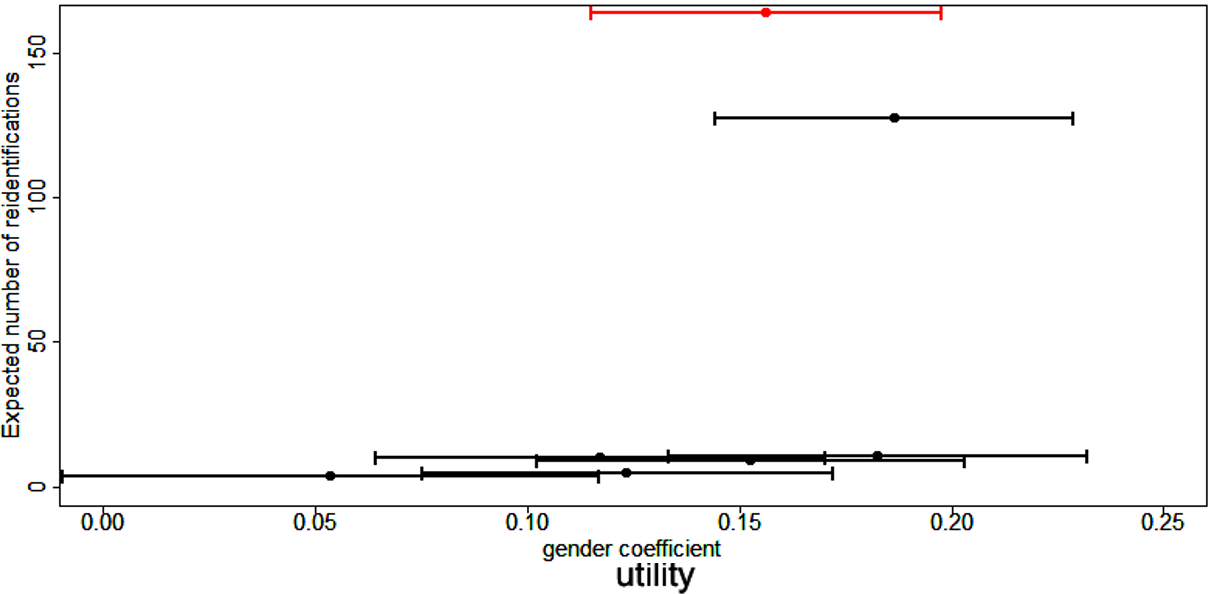
\includegraphics[width=0.9\linewidth]{Imagenes/fig2} 

}

\caption{Efecto de la anonimización en las estimaciones puntuales e intervalo de confianza del coeficiente de género en la ecuación de Mincer.}(\#fig:fig2_sec05)
\end{figure}

\textbf{Fuente:} Imagen extraída de \citep{benschop2021}, pág.90.

\hypertarget{evaluaciuxf3n-de-la-utilidad-de-los-datos-con-la-ayuda-de-visualizaciones-de-datos-en-r}{%
\section{\texorpdfstring{Evaluación de la utilidad de los datos con la ayuda de visualizaciones de datos (en \texttt{R})}{Evaluación de la utilidad de los datos con la ayuda de visualizaciones de datos (en R)}}\label{evaluaciuxf3n-de-la-utilidad-de-los-datos-con-la-ayuda-de-visualizaciones-de-datos-en-r}}

El uso de gráficos y otras técnicas de visualización, actúan como una buena forma de evaluar cuánto han cambiado los datos después de la anonimización ayudando a seleccionar las técnicas de anonimización adecuadas para los datos. Las visualizaciones pueden ser una herramienta útil para evaluar el impacto en la utilidad de los datos de los métodos de anonimización ya que facilitan la elección entre los métodos de anonimización. El lenguaje de programación \texttt{R} proporciona varias funciones y paquetes que pueden ayudar a visualizar los resultados de la
anonimización. Esta sección enumera algunas de estas funciones y paquetes y proporciona ejemplos de código para ilustrar cómo implementarlos. Se mostrarán las siguientes formas:

\begin{itemize}
\tightlist
\item
  histogramas y gráficos de densidad
\item
  diagrama de caja
\item
  gráfico en mosaico
\end{itemize}

Para hacer visualizaciones apropiadas, necesitamos usar los datos sin procesar y los datos anonimizados. Cuando se utiliza un objeto \texttt{sdcMicro} para el proceso de anonimización, los datos sin procesar se almacenan en la ranura ``origData'' del objeto y las variables anonimizadas están en las ranuras ``manipKeyVars'', ``manipPramVars'', ``manipNumVars'' y ``manipStrataVar''. Consulte la sección \protect\hyperlink{objetos-de-la-clase-sdcmicroobj}{Objetos de la clase \texttt{sdcMicroObj}} para obtener más información sobre los objetos \texttt{sdcMicro} , los \emph{slots} y cómo acceder a ellos.

\hypertarget{histogramas-y-gruxe1ficos-de-densidad}{%
\subsubsection{Histogramas y gráficos de densidad}\label{histogramas-y-gruxe1ficos-de-densidad}}

Son útiles para realizar comparaciones rápidas de la distribución de variables antes y después de la anonimización. La ventaja de los histogramas es que los resultados son exactos. Sin embargo, la
visualización depende de los anchos de las barras y el inicio de la primera barra. Los histogramas se pueden utilizar para variables continuas y semicontinuas. Los gráficos de densidad muestran la densidad del kernel de los datos; por lo tanto, la gráfica depende del kernel que se elija y si los datos se ajustan bien al kernel. Sin embargo, los gráficos de densidad son una buena herramienta para ilustrar el cambio de valores y rangos de valores de variables continuas.

Los histogramas se pueden trazar con la función \texttt{hist()} y las densidades del kernel con las funciones \texttt{plot()} y \texttt{density()} en \texttt{R} . El Bloque \ref{exm:bloque11lbn} muestra ejemplos de cómo utilizar estas funciones para ilustrar los cambios en la variable ``INC'', una variable de ingresos. La función \texttt{hist()} necesita como argumento los puntos de ruptura del histograma. Los resultados se muestran en la Figura @ref(fig:fig3\_sec05) y la Figura @ref(fig:fig4\_sec05). Los histogramas y los gráficos de densidad dan una indicación clara de cómo han cambiado los valores: la variabilidad de los datos ha aumentado y la forma de la distribución ha cambiado.

\begin{example}
\protect\hypertarget{exm:bloque11lbn}{}\label{exm:bloque11lbn}Trazado de histogramas y densidades kernel
\end{example}

\begin{Shaded}
\begin{Highlighting}[]
\CommentTok{\# Histograma}
\CommentTok{\# gráfico de histograma antes de la anonimización}
\FunctionTok{hist}\NormalTok{(sdcInitial}\SpecialCharTok{@}\NormalTok{origData}\SpecialCharTok{$}\NormalTok{INC, }\AttributeTok{breaks =}\NormalTok{ (}\DecValTok{0}\SpecialCharTok{:}\DecValTok{180}\NormalTok{)}\SpecialCharTok{*}\FloatTok{1e2}\NormalTok{,}
     \AttributeTok{main =}  \StringTok{"Histogram income {-} original data"}\NormalTok{)}

\CommentTok{\# gráfico de histograma después de la anonimización (adición de ruido)}
\FunctionTok{hist}\NormalTok{(sdcInitial}\SpecialCharTok{@}\NormalTok{manipNumVars}\SpecialCharTok{$}\NormalTok{INC, }\AttributeTok{breaks =}\NormalTok{ (}\SpecialCharTok{{-}}\DecValTok{20}\SpecialCharTok{:}\DecValTok{190}\NormalTok{)}\SpecialCharTok{*}\FloatTok{1e2}\NormalTok{,}
     \AttributeTok{main =} \StringTok{"Histogram income {-} anonymized data"}\NormalTok{)}

\CommentTok{\# gráfico de densidades}
\CommentTok{\# trazo de la curva de densidad original}
\FunctionTok{plot}\NormalTok{(}\FunctionTok{density}\NormalTok{(sdcInitial}\SpecialCharTok{@}\NormalTok{origData}\SpecialCharTok{$}\NormalTok{INC), }\AttributeTok{xlim =} \FunctionTok{c}\NormalTok{(}\DecValTok{0}\NormalTok{, }\DecValTok{8000}\NormalTok{), }\AttributeTok{ylim =} \FunctionTok{c}\NormalTok{(}\DecValTok{0}\NormalTok{, }\FloatTok{0.006}\NormalTok{),}
     \AttributeTok{main =} \StringTok{"Density income"}\NormalTok{, }\AttributeTok{xlab =} \StringTok{"income"}\NormalTok{)}
\FunctionTok{par}\NormalTok{ (}\AttributeTok{new =} \ConstantTok{TRUE}\NormalTok{)}

\CommentTok{\# trazo de la curva de densidad después de la anonimización (adición de ruido)}
\FunctionTok{plot}\NormalTok{(}\FunctionTok{density}\NormalTok{(sdcInitial}\SpecialCharTok{@}\NormalTok{manipNumVars}\SpecialCharTok{$}\NormalTok{INC), }\AttributeTok{xlim =} \FunctionTok{c}\NormalTok{(}\DecValTok{0}\NormalTok{, }\DecValTok{8000}\NormalTok{), }\AttributeTok{ylim =} \FunctionTok{c}\NormalTok{(}\DecValTok{0}\NormalTok{, }\FloatTok{0.006}\NormalTok{),}
     \AttributeTok{main =} \StringTok{"Density income"}\NormalTok{, }\AttributeTok{xlab =} \StringTok{"income"}\NormalTok{)}
\end{Highlighting}
\end{Shaded}

\begin{figure}

{\centering 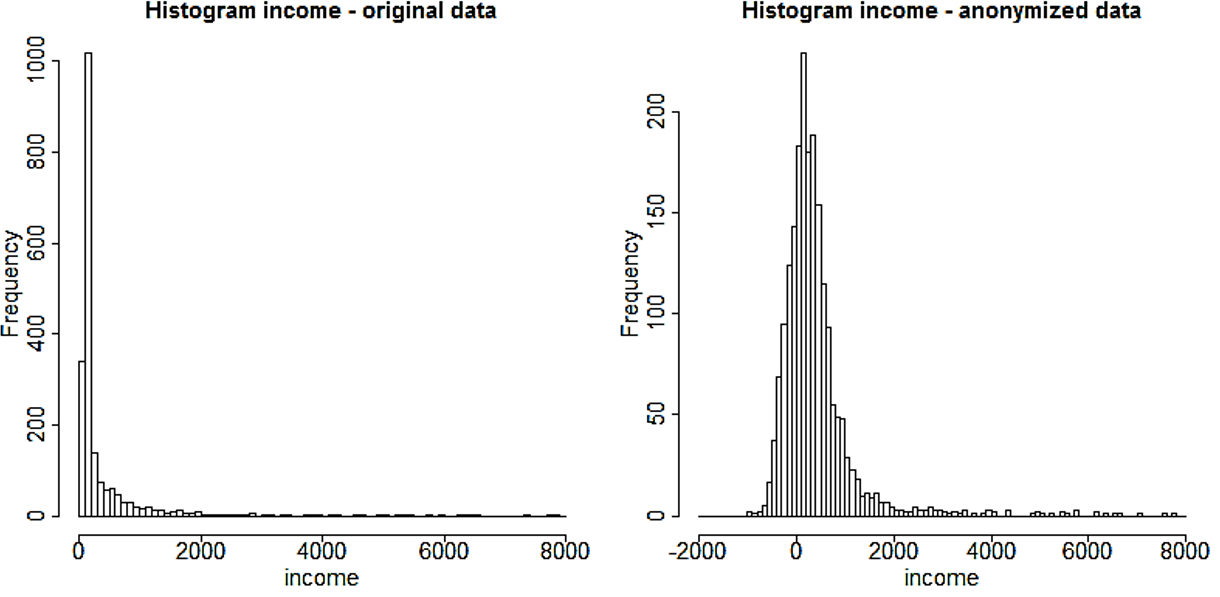
\includegraphics[width=0.9\linewidth]{Imagenes/fig3} 

}

\caption{Histogramas de ingresos antes y después de la anonimización.}(\#fig:fig3_sec05)
\end{figure}

\textbf{Fuente:} Imagen extraída de \citep{benschop2021}, pág.88.

\begin{figure}

{\centering 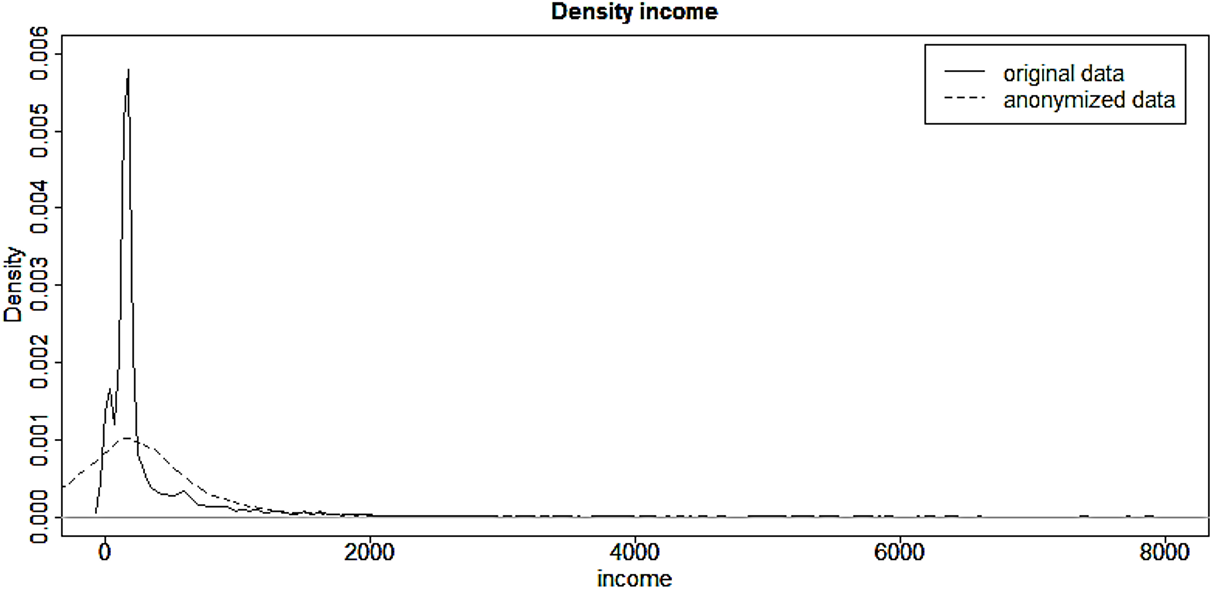
\includegraphics[width=0.9\linewidth]{Imagenes/fig4} 

}

\caption{Gráficas de densidad de ingresos antes y después de la anonimización.}(\#fig:fig4_sec05)
\end{figure}

\textbf{Fuente:} Imagen extraída de \citep{benschop2021}, pág.89.

\hypertarget{diagramas-de-caja}{%
\subsubsection{Diagramas de caja}\label{diagramas-de-caja}}

Los diagramas de caja brindan una descripción general rápida de los cambios en la dispersión y los valores atípicos de las variables continuas antes y después de la anonimización. El Bloque \ref{exm:bloque12lbn} a continuación muestra cómo generar diagramas de caja en \texttt{R} con la función \texttt{boxplot()}. resultado de la figura
@ref(fig:fig5\_sec05) muestra un ejemplo de una variable de gasto después de agregar ruido. El diagrama de caja muestra claramente que la variabilidad en la variable gasto aumentó como resultado de los métodos de anonimización aplicados.

\begin{example}
\protect\hypertarget{exm:bloque12lbn}{}\label{exm:bloque12lbn}Creación de diagramas de caja para variables continuas
\end{example}

\begin{Shaded}
\begin{Highlighting}[]
\FunctionTok{boxplot}\NormalTok{(sdcObj}\SpecialCharTok{@}\NormalTok{origData}\SpecialCharTok{$}\NormalTok{TOTFOOD, sdcObj}\SpecialCharTok{@}\NormalTok{manipNumVars}\SpecialCharTok{$}\NormalTok{TOTFOOD,}
        \AttributeTok{xaxt =} \StringTok{\textquotesingle{}n\textquotesingle{}}\NormalTok{, }\AttributeTok{ylab =} \StringTok{"Expenditure"}\NormalTok{)}
\FunctionTok{axis}\NormalTok{(}\DecValTok{1}\NormalTok{, }\AttributeTok{at =} \FunctionTok{c}\NormalTok{(}\DecValTok{1}\NormalTok{,}\DecValTok{2}\NormalTok{), }\AttributeTok{labels =} \FunctionTok{c}\NormalTok{(}\StringTok{\textquotesingle{}before\textquotesingle{}}\NormalTok{, }\StringTok{\textquotesingle{}after\textquotesingle{}}\NormalTok{))}
\end{Highlighting}
\end{Shaded}

\begin{figure}

{\centering 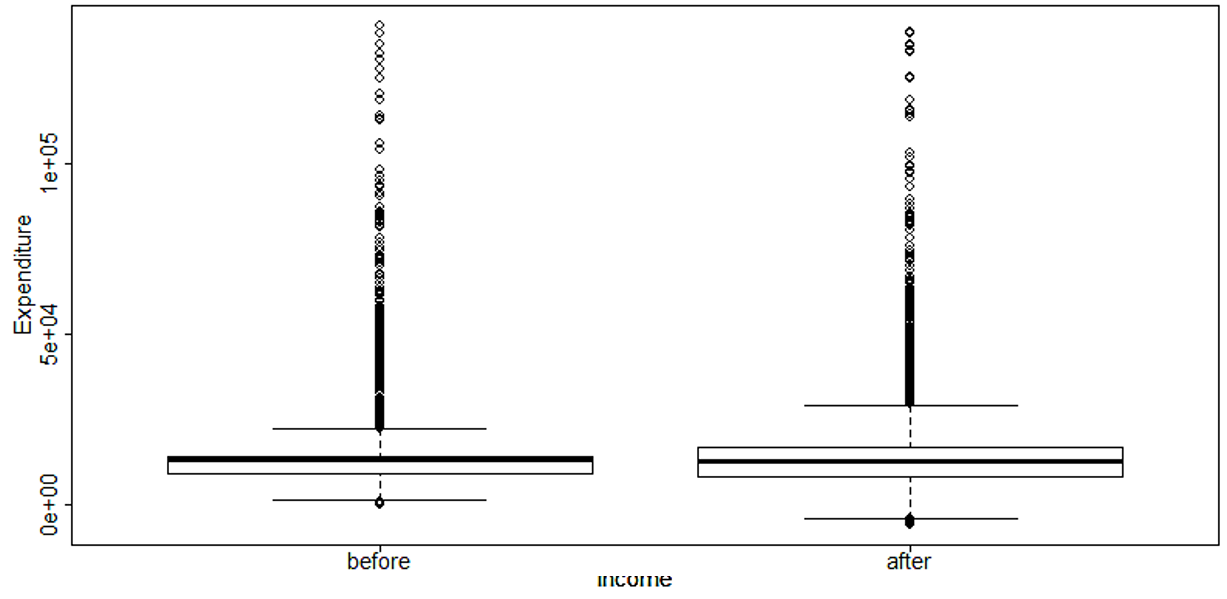
\includegraphics[width=0.9\linewidth]{Imagenes/fig5} 

}

\caption{Ejemplo de diagramas de caja de una variable de gasto antes y después de la anonimización.}(\#fig:fig5_sec05)
\end{figure}

\textbf{Fuente:} Imagen extraída de \citep{benschop2021}, pág.89.

\hypertarget{gruxe1ficos-de-mosaico}{%
\subsubsection{Gráficos de mosaico}\label{gruxe1ficos-de-mosaico}}

Los gráficos de mosaico univariados y multivariados son útiles para mostrar cambios en las tabulaciones de variables categóricas, especialmente cuando se comparan varios ``escenarios'' uno al lado del otro. Un escenario aquí se refiere a la elección de métodos de anonimización y sus parámetros. Con gráficos de mosaico podemos, por
ejemplo, ver rápidamente el efecto de diferentes niveles de k-anonimato o diferencias en los vectores de importancia en el algoritmo de supresión local (ver la Sección \protect\hyperlink{sup-loc}{Supresión local}.

Ilustramos los cambios en las tabulaciones con un ejemplo de la variable ``WATER'' antes y después de aplicar PRAM. Podemos usar gráficos de mosaico para ver rápidamente los cambios de cada categoría. El Bloque \ref{exm:bloque13lbn} muestra el código en \texttt{R} . La función \texttt{mosaicplot()} está disponible en el paquete base de \texttt{R}. Para graficar una tabulación, primero se debe hacer la tabulación con la función \texttt{table()}. Para mostrar las etiquetas en \texttt{mosaicplot()}, cambiamos la clase de las variables a `factor'. Al observar el gráfico de mosaico en la Figura @ref(fig:fig6\_sec05), vemos que la PRAM invariante prácticamente no tiene influencia en la distribución univariante.

\begin{example}
\protect\hypertarget{exm:bloque13lbn}{}\label{exm:bloque13lbn}Creando mosaicos univariados
\end{example}

\begin{Shaded}
\begin{Highlighting}[]
\CommentTok{\# Recopilación de datos de la variable WATER antes y después de la anonimización}
\CommentTok{\# asignación de etiquetas al gráfico}
\NormalTok{dataWater }\OtherTok{\textless{}{-}} \FunctionTok{t}\NormalTok{(}\FunctionTok{cbind}\NormalTok{(}\FunctionTok{table}\NormalTok{(}\FunctionTok{factor}\NormalTok{(sdcHH}\SpecialCharTok{@}\NormalTok{origData}\SpecialCharTok{$}\NormalTok{WATER,}
                                  \AttributeTok{levels =} \FunctionTok{c}\NormalTok{(}\DecValTok{1}\NormalTok{, }\DecValTok{2}\NormalTok{, }\DecValTok{3}\NormalTok{, }\DecValTok{4}\NormalTok{, }\DecValTok{5}\NormalTok{, }\DecValTok{6}\NormalTok{, }\DecValTok{7}\NormalTok{, }\DecValTok{8}\NormalTok{, }\DecValTok{9}\NormalTok{),}
                                  \AttributeTok{labels =} \FunctionTok{c}\NormalTok{(}\StringTok{"Pipe (own tap)"}\NormalTok{, }\StringTok{"Public standpipe"}\NormalTok{,}
                                             \StringTok{"Borehole"}\NormalTok{, }\StringTok{"Wells (protected)"}\NormalTok{,}
                                             \StringTok{"Wells (unprotected)"}\NormalTok{, }\StringTok{"Surface water"}\NormalTok{,}
                                             \StringTok{"Rain water"}\NormalTok{, }\StringTok{"Vendor/truck"}\NormalTok{, }\StringTok{"Other"}\NormalTok{))),}
                     \FunctionTok{table}\NormalTok{(}\FunctionTok{factor}\NormalTok{(sdcHH}\SpecialCharTok{@}\NormalTok{manipPramVars}\SpecialCharTok{$}\NormalTok{WATER,}
                                  \AttributeTok{levels =} \FunctionTok{c}\NormalTok{(}\DecValTok{1}\NormalTok{,}\DecValTok{2}\NormalTok{, }\DecValTok{3}\NormalTok{, }\DecValTok{4}\NormalTok{, }\DecValTok{5}\NormalTok{, }\DecValTok{6}\NormalTok{, }\DecValTok{7}\NormalTok{, }\DecValTok{8}\NormalTok{, }\DecValTok{9}\NormalTok{),}
                                  \AttributeTok{labels =} \FunctionTok{c}\NormalTok{(}\StringTok{"Pipe (own tap)"}\NormalTok{, }\StringTok{"Public standpipe"}\NormalTok{,}
                                             \StringTok{"Borehole"}\NormalTok{, }\StringTok{"Wells (protected)"}\NormalTok{,}
                                             \StringTok{"Wells (unprotected)"}\NormalTok{, }\StringTok{"Surface water"}\NormalTok{,}
                                             \StringTok{"Rain water"}\NormalTok{, }\StringTok{"Vendor/truck"}\NormalTok{,}\StringTok{"Other"}\NormalTok{)))))}
\FunctionTok{rownames}\NormalTok{(dataWater) }\OtherTok{\textless{}{-}} \FunctionTok{c}\NormalTok{(}\StringTok{"before"}\NormalTok{, }\StringTok{"after"}\NormalTok{)}

\CommentTok{\# gráfico de mosaico}
\FunctionTok{mosaicplot}\NormalTok{(dataWater, }\AttributeTok{main =} \StringTok{""}\NormalTok{, }\AttributeTok{color =} \DecValTok{2}\SpecialCharTok{:}\DecValTok{10}\NormalTok{, }\AttributeTok{las =} \DecValTok{2}\NormalTok{)}
\end{Highlighting}
\end{Shaded}

\begin{figure}

{\centering 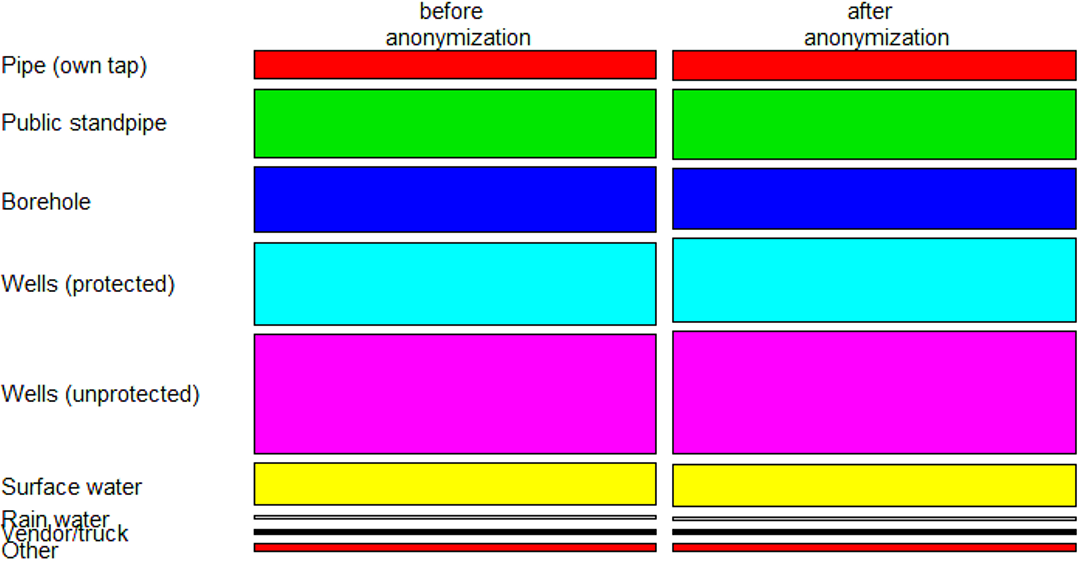
\includegraphics[width=0.9\linewidth]{Imagenes/fig6} 

}

\caption{Gráfico de mosaico para ilustrar los cambios en la variable WATER.}(\#fig:fig6_sec05)
\end{figure}

\textbf{Fuente:} Imagen extraída de \citep{benschop2021}, pág.90.

Usamos las variables ``\emph{gender}'' y ``\emph{relationship status}'' para ilustrar el uso de gráficos de mosaico para la ilustración de cambios en las tabulaciones univariadas introducidas por varios conjuntos de métodos de anonimización. La Tabla \ref{tab:tbl3lbn} proporciona los métodos aplicados en cada escenario. El escenario 0, el escenario base, muestra las categorías originales de las variables de género y estado civil, mientras que los escenarios 1 a 6 muestran cambios en las categorías después de aplicar diferentes técnicas de anonimización. La tabla muestra una descripción de los métodos de anonimización utilizados en cada escenario. En total, visualizamos el impacto de seis conjuntos diferentes de métodos de anonimización. Podemos usar gráficos de mosaico para ver rápidamente qué conjunto de métodos tiene qué impacto en las variables de \emph{gender} y \emph{relationship status}, que se pueden usar para seleccionar el mejor escenario. Mirando los gráficos de mosaico en la Figura @ref(fig:fig7\_sec05), vemos que los escenarios 2, 5 y 6 dan los cambios más pequeños para la variable de \emph{gender} y los escenarios 3 y 4 para la variable de \emph{relationship status}.

\begin{table}

\caption{\label{tab:tbl3lbn}Descripción de métodos de anonimización por escenario}
\begin{tabu} to \linewidth {>{\raggedright}X>{\raggedright}X}
\hline
Escenario & Descripción de los métodos de anonimización aplicados\\
\hline
\textbf{0 (base)} & Datos originales sin tratamiento\\
\hline
\textbf{1} & Recodificar age (intervalos de cinco años), más la supresión local (requerido k = 3, alta importancia en las variables de water, toilet y literacy)\\
\hline
\textbf{2} & Recodificar age (intervalos de cinco años), más supresión local (requerido k = 5, sin vector de importancia)\\
\hline
\textbf{3} & Recodificar la age (intervalos de cinco años), más la supresión local (requerido k = 3, alta importancia en toilet), al mismo tiempo que se recodifican las variables region, urban, education level y ocupation\\
\hline
\textbf{4} & Recodificar age (pasos de cinco años), más supresión local (requerido k = 5, alta importancia en water, toilet, y education level), al mismo tiempo que se recodifican variables de region, urban, education level y ocupation\\
\hline
\textbf{5} & Recodificar age (intervalos de cinco años), más supresión local (requerido k = 3, sin vector de importancia), microagregación (wealth index), al mismo tiempo que se recodifican variables de region, urban, education level y ocupation\\
\hline
\textbf{6} & Recodificar age (intervalos de cinco años) más supresión local (requerido k=3, sin vector de importancia), literacy PRAM, al mismo tiempo que se recodifican variables de region, urban, education level y ocupation\\
\hline
\end{tabu}
\end{table}

\begin{figure}

{\centering 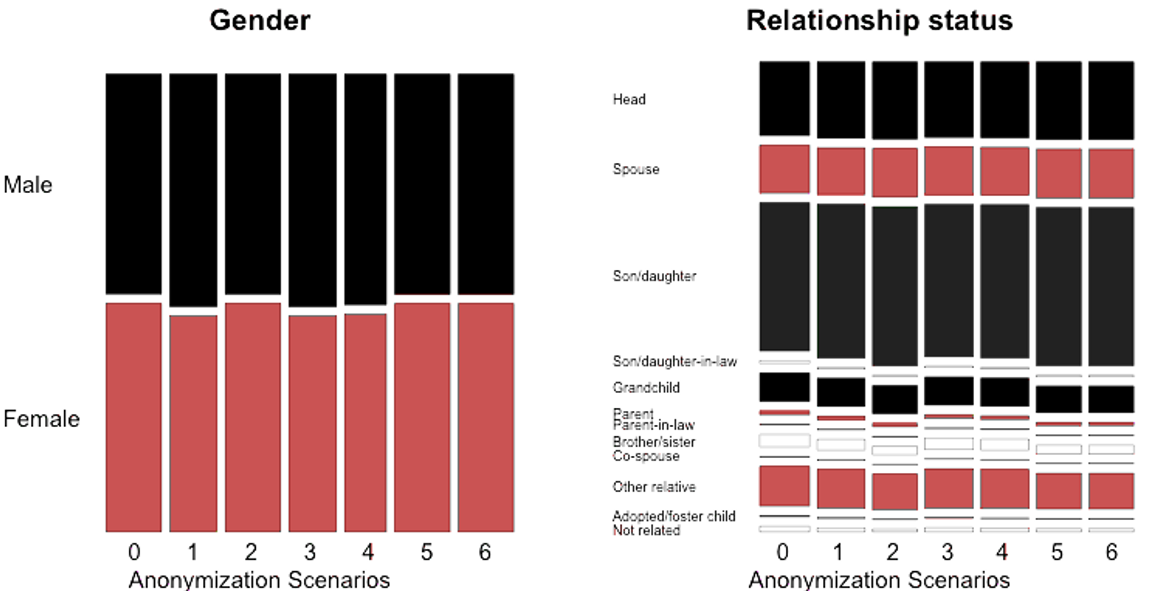
\includegraphics[width=0.9\linewidth]{Imagenes/fig7} 

}

\caption{Comparación de variables de gender y relationship status tratadas versus no tratadas con gráficos de mosaico.}(\#fig:fig7_sec05)
\end{figure}

\textbf{Fuente:} Imagen extraída de \citep{benschop2021}, pág.91

PRAM preserva las distribuciones univariadas. Por lo tanto, en este caso es más interesante observar los gráficos de mosaico multivariado. Los diagramas de mosaico también son una herramienta poderosa para mostrar cambios en
tabulaciones cruzadas/tablas de contingencia. El Bloque \ref{exm:bloque14lbn} a continuación muestra cómo generar gráficos de mosaico para dos variables. Para comparar los cambios, necesitamos comparar dos gráficos diferentes. La Figura @ref(fig:fig8\_sec05) y la Figura @ref(fig:fig9\_sec05) ilustran que la PRAM no conserva las tablas
de doble entrada en este caso.

\begin{example}
\protect\hypertarget{exm:bloque14lbn}{}\label{exm:bloque14lbn}Creando mosaicos multivariados
\end{example}

\begin{Shaded}
\begin{Highlighting}[]
\CommentTok{\# Antes de la anonimización: tabla de contingencia y gráfico de mosaico}
\NormalTok{ROOFTOILETbefore }\OtherTok{\textless{}{-}} \FunctionTok{t}\NormalTok{(}\FunctionTok{table}\NormalTok{(}\FunctionTok{factor}\NormalTok{(sdcHH}\SpecialCharTok{@}\NormalTok{origData}\SpecialCharTok{$}\NormalTok{ROOF, }\AttributeTok{levels =} \FunctionTok{c}\NormalTok{(}\DecValTok{1}\NormalTok{,}\DecValTok{2}\NormalTok{, }\DecValTok{3}\NormalTok{, }\DecValTok{4}\NormalTok{, }\DecValTok{5}\NormalTok{, }\DecValTok{9}\NormalTok{),}
                                   \AttributeTok{labels =} \FunctionTok{c}\NormalTok{(}\StringTok{"Concrete/cement/ }\SpecialCharTok{\textbackslash{}n}\StringTok{ brick/stone"}\NormalTok{, }\StringTok{"Wood"}\NormalTok{,}
                                              \StringTok{"Bamboo/thatch"}\NormalTok{, }\StringTok{"Tiles/shingles"}\NormalTok{,}
                                              \StringTok{"Tin/metal sheets"}\NormalTok{, }\StringTok{"Other"}\NormalTok{)),}
                            \FunctionTok{factor}\NormalTok{(sdcHH}\SpecialCharTok{@}\NormalTok{origData}\SpecialCharTok{$}\NormalTok{TOILET, }\AttributeTok{levels =} \FunctionTok{c}\NormalTok{(}\DecValTok{1}\NormalTok{,}\DecValTok{2}\NormalTok{, }\DecValTok{3}\NormalTok{, }\DecValTok{4}\NormalTok{, }\DecValTok{9}\NormalTok{),}
                                   \AttributeTok{labels =} \FunctionTok{c}\NormalTok{(}\StringTok{"Flush }\SpecialCharTok{\textbackslash{}n}\StringTok{ toilet"}\NormalTok{,}
                                              \StringTok{"Improved }\SpecialCharTok{\textbackslash{}n}\StringTok{ pit }\SpecialCharTok{\textbackslash{}n}\StringTok{ latrine"}\NormalTok{,}
                                              \StringTok{"Pit }\SpecialCharTok{\textbackslash{}n}\StringTok{ latrine"}\NormalTok{, }\StringTok{"No }\SpecialCharTok{\textbackslash{}n}\StringTok{ facility"}\NormalTok{,}
                                              \StringTok{"Other"}\NormalTok{))))}
\FunctionTok{mosaicplot}\NormalTok{(ROOFTOILETbefore, }\AttributeTok{main =} \StringTok{""}\NormalTok{, }\AttributeTok{las =} \DecValTok{2}\NormalTok{, }\AttributeTok{color =} \DecValTok{2}\SpecialCharTok{:}\DecValTok{6}\NormalTok{)}

\CommentTok{\# Después de la anonimización: tabla de contingencia y gráfico de mosaico}
\NormalTok{ROOFTOILETafter }\OtherTok{\textless{}{-}} \FunctionTok{t}\NormalTok{(}\FunctionTok{table}\NormalTok{(}\FunctionTok{factor}\NormalTok{(sdcHH}\SpecialCharTok{@}\NormalTok{manipPramVars}\SpecialCharTok{$}\NormalTok{ROOF, }\AttributeTok{levels =} \FunctionTok{c}\NormalTok{(}\DecValTok{1}\NormalTok{,}\DecValTok{2}\NormalTok{, }\DecValTok{3}\NormalTok{, }\DecValTok{4}\NormalTok{, }\DecValTok{5}\NormalTok{, }\DecValTok{9}\NormalTok{),}
                                  \AttributeTok{labels =} \FunctionTok{c}\NormalTok{(}\StringTok{"Concrete/cement/ }\SpecialCharTok{\textbackslash{}n}\StringTok{ brick/stone"}\NormalTok{, }\StringTok{"Wood"}\NormalTok{,}
                                             \StringTok{"Bamboo/thatch"}\NormalTok{, }\StringTok{"Tiles/shingles"}\NormalTok{,}
                                             \StringTok{"Tin/metal sheets"}\NormalTok{, }\StringTok{"Other"}\NormalTok{)),}
                           \FunctionTok{factor}\NormalTok{(sdcHH}\SpecialCharTok{@}\NormalTok{manipPramVars}\SpecialCharTok{$}\NormalTok{TOILET, }\AttributeTok{levels =} \FunctionTok{c}\NormalTok{(}\DecValTok{1}\NormalTok{,}\DecValTok{2}\NormalTok{, }\DecValTok{3}\NormalTok{, }\DecValTok{4}\NormalTok{, }\DecValTok{9}\NormalTok{),}
                                  \AttributeTok{labels =} \FunctionTok{c}\NormalTok{(}\StringTok{"Flush }\SpecialCharTok{\textbackslash{}n}\StringTok{ toilet"}\NormalTok{,}
                                             \StringTok{"Improved }\SpecialCharTok{\textbackslash{}\textbackslash{}}\StringTok{n pit }\SpecialCharTok{\textbackslash{}n}\StringTok{ latrine"}\NormalTok{,}
                                             \StringTok{"Pit }\SpecialCharTok{\textbackslash{}n}\StringTok{ latrine"}\NormalTok{, }\StringTok{"No }\SpecialCharTok{\textbackslash{}n}\StringTok{ facility"}\NormalTok{,}
                                             \StringTok{"Other"}\NormalTok{))))}
\FunctionTok{mosaicplot}\NormalTok{(ROOFTOILETafter, }\AttributeTok{main =} \StringTok{""}\NormalTok{, }\AttributeTok{las =} \DecValTok{2}\NormalTok{, }\AttributeTok{color =} \DecValTok{2}\SpecialCharTok{:}\DecValTok{6}\NormalTok{)}
\end{Highlighting}
\end{Shaded}

\begin{figure}

{\centering 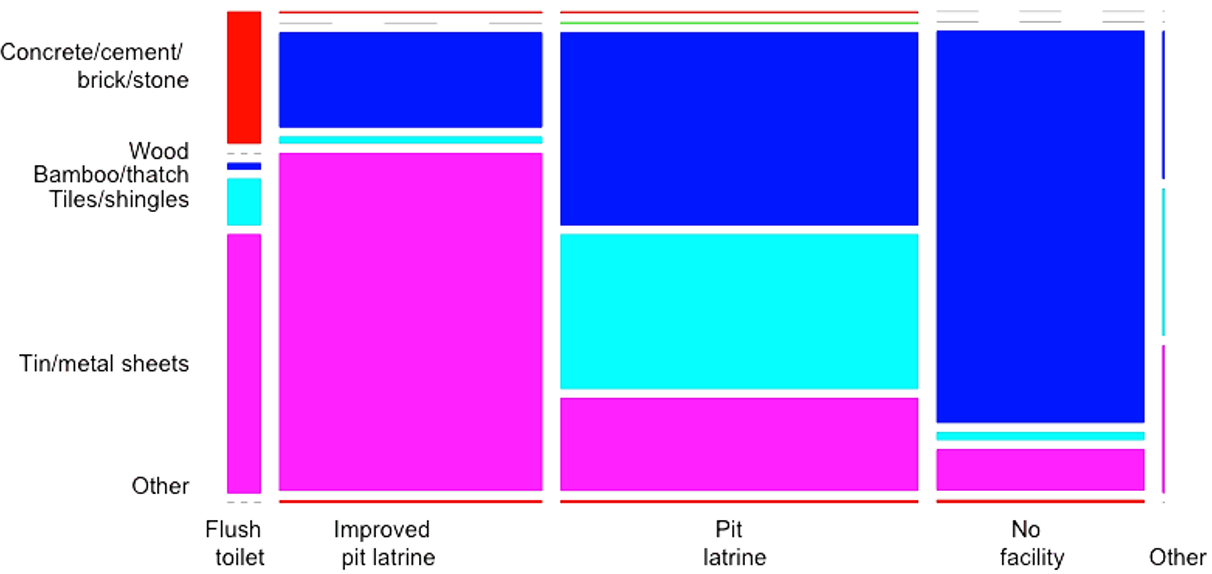
\includegraphics[width=0.9\linewidth]{Imagenes/fig8} 

}

\caption{Gráfico de mosaico de las variables ROOF e TOILET antes de la anonimización.}(\#fig:fig8_sec05)
\end{figure}

\textbf{Fuente:} Imagen extraída de \citep{benschop2021},pág. 92.

\begin{figure}

{\centering 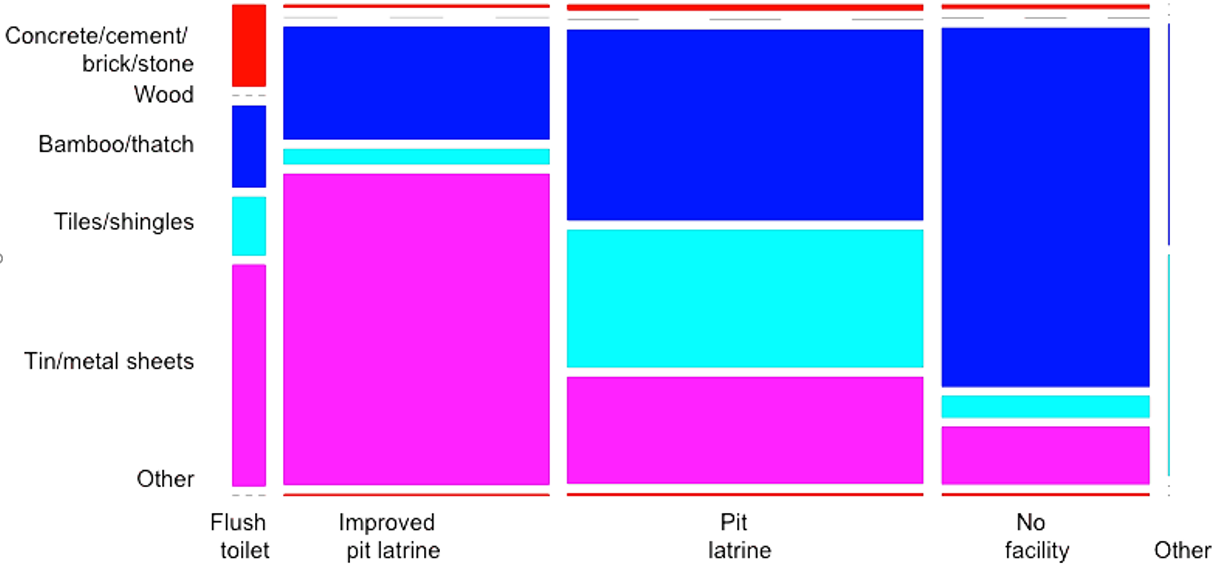
\includegraphics[width=0.9\linewidth]{Imagenes/fig9} 

}

\caption{Gráfico de mosaico de las variables ROOF e TOILET después de la anonimización.}(\#fig:fig9_sec05)
\end{figure}

\textbf{Fuente:} Imagen extraída de \citep{benschop2021}, pág.93.

\hypertarget{elecciuxf3n-de-la-medida-de-utilidad}{%
\subsection{Elección de la medida de utilidad}\label{elecciuxf3n-de-la-medida-de-utilidad}}

Además de los requisitos de los usuarios sobre los datos, las medidas de utilidad deben elegirse de acuerdo con los tipos de variables y los métodos de anonimización empleados. Las medidas de utilidad empleadas pueden ser una combinación de medidas generales y específicas del usuario. Como se discutió anteriormente, se deben usar diferentes medidas de utilidad para datos continuos y categóricos. Además, algunas medidas de utilidad no son informativas después de que se hayan aplicado ciertos métodos de anonimización. Por ejemplo, después de aplicar
métodos perturbativos que intercambian valores de datos, la comparación directa de valores no es útil porque dará la impresión de altos niveles de pérdida de información. En tales casos, es más informativo observar
las medias, las covarianzas y los indicadores de evaluación comparativa que se pueden calcular a partir de los datos. Es más, es importante no solo centrarse en las características de las variables una por una, sino
también en las interacciones entre las variables. Esto se puede hacer mediante tabulaciones cruzadas y regresiones. En general, al anonimizar datos muestreados, es recomendable calcular intervalos de confianza
alrededor de las estimaciones para interpretar la magnitud de los cambios.

\begin{quote}
\textbf{Nota:} Para material de lectura recomendado sobre la medición de la
utilidad y la pérdida de información ver \citep{dewaal1999}, \citep{domingo-ferrer2001} y \citep{domingo-ferrer2001}.
\end{quote}

\hypertarget{proceso-control-a-la-divulgaciuxf3n-estaduxedstica-sdc-ine-2021}{%
\chapter{Proceso Control a la Divulgación Estadística (SDC) INE 2021}\label{proceso-control-a-la-divulgaciuxf3n-estaduxedstica-sdc-ine-2021}}

\hypertarget{introducciuxf3n-2}{%
\section{Introducción}\label{introducciuxf3n-2}}

Esta sección presenta el proceso SDC en una representación paso a paso y se puede utilizar como guía para el proceso SDC real, de acuerdo con los lineamientos INE 2021 (ver \citep{ine2021}). Sin embargo, debe tenerse en cuenta que, a menudo, es necesario saltar de un paso a otro y volver a los pasos anteriores durante el proceso SDC real, ya que no es necesariamente un proceso lineal paso a paso. Esta guía reúne las diferentes partes del proceso SDC como se discutió en las secciones anteriores y los enlaces a estas secciones. El estudio de caso en la siguiente sección sigue estos pasos. La Figura \ref{fig:esquemaSDC} al final de esta sección presenta todo el proceso de forma esquemática.

\hypertarget{etapa-6.4.1-definiciones-previas-al-proceso-de-anonimizaciuxf3n}{%
\section{Etapa 6.4.1: Definiciones previas al proceso de anonimización}\label{etapa-6.4.1-definiciones-previas-al-proceso-de-anonimizaciuxf3n}}

El propósito de esta etapa es establecer los requerimientos necesarios para iniciar el subproceso de control a la divulgación, que incluye la revisión de insumos, revisión de las necesidades de los usuarios y características estadísticas prioritarias, y la determinación de la necesidad de protección de confidencialidad. Esto último, está estrechamente relacionado con la interpretación de las leyes y normas sobre este tema en Chile.

Los procedimientos descritos para esta etapa aplican para todas las operaciones estadísticas y productos relacionados cuyo levantamiento de información y/o publicación sea realizado por el INE (muestras, censos, procesos de múltiples fuentes y registros estadísticos) que darán a conocer información al público general u otros usuarios.
En esta etapa se debe revisar que no existan restricciones legales que impidan la publicación de los microdatos.
Por otra parte, si el conjunto de datos no posee variables sensibles o variables de identificación (directa o indirecta), se pasa a la \protect\hyperlink{etapa-6.4.5-generar-reportes-y-liberar-datos}{Etapa 6.4.5: Generar reportes y liberar datos}.

\hypertarget{definiciones-previas}{%
\subsection{Definiciones previas}\label{definiciones-previas}}

\begin{itemize}
\item
  \textbf{Organización del proceso y equipo de trabajo}: El trabajo del proceso SDC y los roles del equipo a cargo se deben organizar considerando las siguientes dos fases: diagnóstico e implementación. La fase de diagnóstico corresponde a la evaluación de riesgo de intrusión con los datos no tratados (originales o brutos), y permite juzgar si el conjunto de datos es lo suficientemente seguro para su publicación, mientras que la fase de implementación se refiere a la aplicación de métodos SDC y su evaluación, a fin de producir un conjunto de datos seguro para su publicación.
\item
  \textbf{Revisión de insumos o productos estadísticos necesarios que permiten la ejecución del proceso}: Se debe revisar que los insumos o productos estadísticos provenientes de los siguientes procesos en el mapa de procesos INE, segmento negocios\footnote{Disponible en \url{https://inechile.sharepoint.com/sites/Intranet/departamentodegestionestrategica/Mprocesos/Paginas/Segmento-Negocio.aspx}}: 2. ``Diseño y planificación'', 5. ``Procesamiento'' y 6.3 ``Interpretar y explicar los resultados''; necesarios para la ejecución de este subproceso, se encuentren completos y actualizados. Esto incluye la revisión de convenios, fichas metodológicas, manuales de usuarios, bases de datos, diccionario de variables, paquetes estadísticos, infraestructura y seguridad, entre otros.
\end{itemize}

\hypertarget{determinaciuxf3n-de-la-necesidad-de-protecciuxf3n-de-la-confidencialidad}{%
\subsection{Determinación de la necesidad de protección de la confidencialidad}\label{determinaciuxf3n-de-la-necesidad-de-protecciuxf3n-de-la-confidencialidad}}

Antes de iniciar el proceso SDC para un conjunto de microdatos, se debe determinar la necesidad de protección de la confidencialidad. Esto está estrechamente relacionado con la interpretación de las leyes y reglamentos sobre este tema en Chile. Un primer paso es determinar las unidades estadísticas en el conjunto de datos: si se trata de individuos, hogares o entidades legales, como empresas, es probable que sea necesario controlar la divulgación. También hay ejemplos de microdatos para los que no hay necesidad de control de divulgación. Los ejemplos podrían ser datos con observaciones climáticas y meteorológicas o datos con viviendas como unidades estadísticas. Sin embargo, aunque las unidades estadísticas primarias no sean personas físicas o jurídicas, los datos pueden contener información confidencial sobre personas físicas o jurídicas. Por ejemplo, un conjunto de datos con viviendas como unidades estadísticas primarias también puede contener información sobre las personas que viven en estas viviendas y sus ingresos o un conjunto de datos sobre hospitalizaciones puede incluir información sobre los pacientes hospitalizados. En estos casos, es probable que todavía sea necesaria la protección de la confidencialidad. Una opción para resolver esto es eliminar la información sobre las personas físicas y jurídicas en los conjuntos de datos para su publicación.

Un conjunto de datos también puede contener más de un tipo de unidad estadística. El ejemplo estándar aquí es un conjunto de datos que contiene información sobre individuos y hogares. Otro ejemplo son los datos con empleados en empresas. Todos los tipos de unidades estadísticas presentes en el conjunto de datos deben ser considerados para la necesidad de SDC. Esto es especialmente importante en caso de que los datos tengan una estructura jerárquica, como individuos en hogares o empleados en empresas.

Además, se debe evaluar si las variables contenidas en el conjunto de datos son de identificación, confidenciales o sensibles. Qué variables son sensibles o confidenciales depende nuevamente de la legislación aplicable y puede diferir sustancialmente de un país a otro. En caso de que el conjunto de datos incluya variables sensibles o confidenciales, es probable que se requiera SDC. El conjunto de variables sensibles y variables de identificación junto con las unidades estadísticas en el conjunto de datos determinan la necesidad de control de divulgación estadística.

Por otra parte, se debe realizar una revisión normativa que pueda afectar o impedir la publicación de la información sujeta a anonimizar, esto incluye: identificar las restricciones actuales de publicación de la información, identificar acuerdos y restricciones de las particularidades establecidas en los convenios del INE con fuentes externas.

Si no existen variables sensibles o variables de identificación en el conjunto de datos, o restricciones desde el marco legal normativo, la decisión es pasar a la \protect\hyperlink{etapa-6.4.5-generar-reportes-y-liberar-datos}{Etapa 6.4.5: Generar reportes y liberar datos}, según las características establecidas en la metodología de la operación estadística o convenio institucional, según corresponda a lo establecido en el proceso 2. ``Diseño y planificación''. Por el contrario, en caso de que el conjunto de datos contenga variables sensibles o variables de identificación, y no haya restricciones desde el marco legal normativo, la decisión es llevar a cabo un proceso SDC.

\hypertarget{definiciuxf3n-de-las-caracteruxedsticas-de-las-bases-de-datos-a-preservar}{%
\subsection{Definición de las características de las bases de datos a preservar}\label{definiciuxf3n-de-las-caracteruxedsticas-de-las-bases-de-datos-a-preservar}}

En este paso, analizamos los principales usos de los datos por parte de los usuarios finales del archivo de microdatos publicado. Los datos deben ser útiles para el tipo de análisis estadístico para el que se recopilaron y para el que se utilizan principalmente. Los usos y requisitos de los usuarios de datos serán diferentes para los diferentes tipos de publicación. Ponerse en contacto directamente con los usuarios de datos o buscar estudios y artículos científicos que utilicen datos similares puede resultar útil a la hora de recopilar esta información y realizar esta evaluación. Además, es importante comprender qué nivel de precisión necesitan los usuarios de datos y qué tipos de categorías se utilizan. Por ejemplo, en el caso de la recodificación global de la edad en años, uno podría recodificar la edad en grupos de 10 años, por ejemplo, \(0 – 9, 10 – 19, 20 – 29, ...\). Sin embargo, muchos indicadores relacionados con el mercado laboral usan categorías que abarcan el rango 15 -- 65. Por lo tanto, construir categorías que coincidan con las categorías utilizadas para los indicadores hace que los datos sean mucho más útiles y, al mismo tiempo, reduce el riesgo de divulgación de manera similar. Este conocimiento es importante para la selección de medidas de utilidad apropiadas, que a su vez se utilizan para seleccionar los métodos SDC apropiados.

La anonimización siempre conducirá a la pérdida de información y un archivo PUF tendrá una utilidad reducida.

Las estadísticas calculadas a partir del archivo de microdatos anonimizados y publicados deberían producir resultados analíticos que concuerdan o casi concuerdan con las estadísticas publicadas previamente a partir de los datos originales. Si, por ejemplo, se calculó el promedio de ingresos de los hogares chilenos previamente a partir de estos datos y se publicó, el conjunto de datos anónimos publicado debería producir un resultado muy similar al resultado publicado oficialmente. Como mínimo, el resultado debe estar dentro de la región de confianza del resultado publicado. Puede darse el caso de que no todas las estadísticas publicadas puedan generarse a partir de los datos publicados. Si este es el caso, se debe elegir en qué indicadores y estadísticas enfocarse, e informar a los usuarios sobre cuáles se han seleccionado y por qué. Además, es importante definir porcentajes de variación permitidos por variable y niveles de desagregación geográfica o temática para las características estadísticas, a fin de medir la utilidad que compara los datos originales y los datos anonimizados, teniendo en cuenta la necesidad del usuario final para su análisis.

Algunos ejemplos de características estadísticas a preservar son las siguientes:

\begin{itemize}
\tightlist
\item
  Propiedades globales de las variables, como promedios.
\item
  Mantener cifras por nivel de desagregación geográfica o temática, como, por ejemplo, mantener para la variable grupos étnicos en los totales de cada categoría a nivel regional.
\item
  Mantener correlaciones entre variables.
\item
  Mantener tendencias de las variables a través del tiempo, por ejemplo, si los ingresos promedio de los hogares chilenos ha presentado un comportamiento decreciente en el primer trimestre de 2021, al publicar la base de datos anonimizada el equipo de trabajo desea garantizar que esta tendencia se conserve.
\end{itemize}

Como se discutió en la Sección \protect\hyperlink{mediciuxf3n-de-la-utilidad-y-la-puxe9rdida-de-informaciuxf3n}{Medición de la utilidad y la pérdida de información}, es necesario calcular medidas generales de utilidad que comparen los datos sin procesar y anonimizados, teniendo en cuenta la necesidad del usuario final para su análisis. En algunos casos, las medidas de utilidad pueden arrojar resultados contradictorios, por ejemplo, un determinado método SDC podría generar una menor pérdida de información para las cifras de la fuerza laboral pero una mayor pérdida de información para los índices relacionados con la educación. En tales casos, es posible que sea necesario clasificar los usos de los datos en orden de importancia y se debe documentar claramente para el usuario que la priorización de ciertas métricas sobre otras significa hará que algunas métricas ya no sean válidas. Esto puede ser necesario, ya que no es posible liberar varios archivos para diferentes usuarios. Este problema se presenta especialmente en estudios polivalentes. Para obtener más detalles sobre las medidas de utilidad, consulte la Sección \protect\hyperlink{mediciuxf3n-de-la-utilidad-y-la-puxe9rdida-de-informaciuxf3n}{Medición de la utilidad y la pérdida de información}.

\hypertarget{etapa-6.4.2-preparaciuxf3n-y-exploraciuxf3n-de-datos}{%
\section{Etapa 6.4.2: Preparación y exploración de datos}\label{etapa-6.4.2-preparaciuxf3n-y-exploraciuxf3n-de-datos}}

Después de evaluar la necesidad de un control de divulgación estadística, debemos preparar los datos y, si hay varios, combinar y considerar todos los archivos de datos relacionados. Luego exploramos las características y la estructura de los datos, que son importantes para los usuarios de los datos. La compilación de un inventario de estas características es importante para evaluar la utilidad de los datos después de la anonimización y producir un conjunto de datos anonimizados, que es útil para los usuarios finales.

El primer paso en la preparación de datos es clasificar las variables como confidenciales o no confidenciales y eliminar identificadores directos como nombres completos, números de pasaporte, direcciones, números de teléfono y coordenadas GPS. En el caso de datos de encuestas, una inspección del cuestionario de la encuesta es útil para clasificar las variables. Además, es necesario seleccionar las variables que contienen información relevante para los usuarios finales y deben incluirse en el conjunto de datos para su publicación. En este punto, también puede ser útil eliminar variables que no sean identificadores directos del conjunto de microdatos que se publicará. Un ejemplo puede ser una variable con muchos valores faltantes, por ejemplo, una variable registrada solo para un grupo selecto de personas elegibles para un módulo de encuesta en particular y valores faltantes para el resto. Tales variables pueden causar un alto nivel de riesgo de divulgación y agregar poca información para los usuarios finales. Ejemplos son variables relacionadas con la educación (grado actual), donde un valor faltante indica que la persona no está actualmente en la escuela, o variables relacionadas con el parto, donde un valor faltante indica que la persona no ha dado a luz en el período de referencia. Los valores faltantes en sí mismos pueden ser reveladores, especialmente si indican que la variable no es aplicable. A menudo, las variables a las que les faltan la mayoría de los valores ya se eliminan en esta etapa. Otras variables que podrían eliminarse en esta etapa son aquellas demasiado sensibles para anonimizarlas y difundirlas o aquellas que no son importantes para los usuarios de datos y que podrían aumentar el riesgo de divulgación.

Las relaciones pueden existir entre las variables en un conjunto de datos por una variedad de razones. Por ejemplo, las variables pueden ser mutuamente excluyentes en los casos en que se utilizan varias variables binarias para cada categoría. Un individuo que no está en la fuerza laboral tendrá un valor faltante para el sector en el que esta persona está empleada (o, más precisamente, no aplicable). Las relaciones también pueden existir si algunas variables son proporciones, sumas u otras funciones matemáticas de otras variables. Algunos ejemplos son la variable tamaño del hogar (como un recuento de personas por hogar) o el gasto agregado (como la suma de todos los componentes del gasto). Un cierto valor en una variable también puede reducir el número de valores posibles o válidos para otra variable; por ejemplo, la edad de una persona que asiste a la educación primaria o el sexo de una persona que ha dado a luz. Estas relaciones son importantes por dos razones: 1) pueden ser utilizadas por intrusos para reconstruir valores anonimizados. Por ejemplo, si se suprime la edad pero otra variable indica que está en la escuela, aún es posible inferir un rango de edad probable para ese individuo. Otro ejemplo es si se demuestra que un individuo está activo en el Sector B de la economía. Incluso si se suprime la condición laboral de este individuo, se puede inferir que esta persona está empleada. 2) las relaciones en los datos originales deben mantenerse en el conjunto de datos anonimizados y deben evitarse las inconsistencias (por ejemplo, los métodos SDC no deben crear niños en edad escolar de 58 años o niños casados de 3 años), o el conjunto de datos será inválido para el análisis. Otro ejemplo es el caso de los gastos por categoría, donde es importante que la suma de las categorías sume el total. Una forma de garantizar esto es anonimizar los totales y luego recalcular las subcategorías de acuerdo con las acciones originales de los totales anónimos.

También es útil en esta etapa consolidar variables que brinden la misma información cuando sea posible, para reducir el número de variables, reducir la probabilidad de inconsistencias y minimizar las variables que un intruso puede usar para reconstruir los datos. Esto es especialmente cierto si los microdatos provienen de un cuestionario elaborado y cada variable representa una (sub) pregunta que conduce a un conjunto de datos con cientos de variables. Como ejemplo, tomamos una encuesta con varias variables de fuerza laboral que indican si una persona está en la fuerza laboral, empleada o desempleada, y si está empleada, en qué sector. Los datos de la Tabla \ref{tab:tabProc1} ilustra este ejemplo. Es posible que cada tipo de sector tenga su propia variable binaria. En ese caso, este conjunto de variables se puede resumir en dos variables: una variable que indica si una persona está en la fuerza laboral y otra que indica la situación laboral, así como el sector respectivo si una persona está empleada. Estas dos variables contienen toda la información contenida en las cinco variables anteriores y facilitan el proceso de anonimización. Si los usuarios de datos están acostumbrados a un determinado formato de publicación en el que la norma ha sido incluir las cinco variables, entonces es posible volver a transformar las variables después del proceso de anonimización en lugar de complicar el proceso de anonimización tratando de tratar más variables de las necesarias.

\begin{table}

\caption{\label{tab:tabProc1}Ilustración de la combinación de variables sin pérdida de información para el proceso SDC.}
\centering
\begin{tabular}[t]{c|c|c|c|c|c|c}
\hline
FL-Orig & Empleado-Orig & Sector-A & Sector-B & Sector-C & FL-Nueva & Empleado-Nueva\\
\hline
Sí & Sí & NA & Sí & NA & Sí & B\\
\hline
No & No & NA & NA & NA & No & No\\
\hline
Sí & Sí & Sí & NA & NA & Sí & A\\
\hline
Sí & Sí & NA & Sí & NA & Sí & B\\
\hline
Sí & Sí & NA & NA & Sí & Sí & C\\
\hline
Sí & No & NA & NA & NA & Sí & No\\
\hline
\end{tabular}
\end{table}

\begin{quote}
\textbf{Nota sobre los pasos siguientes}:
Los siguientes pasos, \protect\hyperlink{etapa-6.4.3-mediciuxf3n-y-evaluaciuxf3n-de-riesgos-de-divulgaciuxf3n}{Etapa 6.4.3: Medición y evaluación de riesgos de divulgación}, \protect\hyperlink{etapa-6.4.4.1-selecciuxf3n-y-aplicaciuxf3n-de-muxe9todos-sdc}{Etapa 6.4.4.1: Selección y aplicación de métodos SDC} y \protect\hyperlink{etapa-6.4.4.2-evaluaciuxf3n-de-proceso-sdc}{Etapa 6.4.4.2: Evaluación de proceso SDC}, deben repetirse si los datos tienen identificadores indirectos que se encuentran en diferentes niveles jerárquicos, por ejemplo, individuo y hogar. En ese caso, las variables del nivel jerárquico superior deben anonimizarse primero y luego fusionarse con las variables no tratadas del nivel inferior. Posteriormente, el conjunto de datos combinado debe anonimizarse. Este enfoque garantiza la consistencia en los datos tratados. Si descuidamos este procedimiento, los valores de las variables medidas en el nivel jerárquico superior podrían recibir un tratamiento diferente para las observaciones de la misma unidad. Por ejemplo, la variable ``región'' es la misma para todos los miembros del hogar. Si se suprimiera el valor `Valparaíso' para dos miembros pero no para los tres restantes, esto daría lugar a una divulgación no intencionada; con la identificación del hogar, la variable región sería fácil de reconstruir para los dos valores suprimidos. Las secciones \protect\hyperlink{riesgo-jeruxe1rquico-o-del-hogar}{Riesgo jerárquico (o del hogar)} y \protect\hyperlink{estructura-del-hogar}{Estructura del hogar} brindan más detalles sobre cómo tratar los datos con la estructura del hogar en \texttt{R} y \texttt{sdcMicro} .
\end{quote}

\hypertarget{etapa-6.4.3-mediciuxf3n-y-evaluaciuxf3n-de-riesgos-de-divulgaciuxf3n}{%
\section{Etapa 6.4.3: Medición y evaluación de riesgos de divulgación}\label{etapa-6.4.3-mediciuxf3n-y-evaluaciuxf3n-de-riesgos-de-divulgaciuxf3n}}

El propósito de esta etapa es calcular medidas de riesgo sobre los datos originales o brutos y, en base a estas medidas, juzgar si un archivo de microdatos es lo suficientemente seguro para su publicación.

Los procedimientos descritos para esta etapa aplican para todas las operaciones estadísticas y productos relacionados cuyo levantamiento de información y/o publicación sea realizado por el INE (encuestas, censos, procesos de múltiples fuentes y registros administrativos) que darán a conocer información al público general u otros usuarios.

En esta etapa solo se calculan las medidas de riesgo sobre los datos originales, que permiten decidir si el archivo de microdatos es lo suficientemente seguro para su publicación, o si requiere la aplicación de métodos SDC (ver \protect\hyperlink{etapa-6.4.4.1-selecciuxf3n-y-aplicaciuxf3n-de-muxe9todos-sdc}{Etapa 6.4.4.1: Selección y aplicación de métodos SDC}). La decisión sobre qué hacer con las unidades riesgosas (una vez aplicados los métodos SDC) se aborda en la \protect\hyperlink{etapa-6.4.4.2-evaluaciuxf3n-de-proceso-sdc}{Etapa 6.4.4.2: Evaluación de proceso SDC}.

\hypertarget{definiciuxf3n-de-escenarios-de-divulgaciuxf3n-y-selecciuxf3n-de-identificadores-indirectos-cuasi-identificadores-o-variables-clave}{%
\subsection{Definición de escenarios de divulgación y selección de identificadores indirectos (cuasi-identificadores o variables clave)}\label{definiciuxf3n-de-escenarios-de-divulgaciuxf3n-y-selecciuxf3n-de-identificadores-indirectos-cuasi-identificadores-o-variables-clave}}

Después de determinar el tipo de publicación de los datos, se deben examinar las posibilidades de cómo un individuo en los microdatos podría (de manera realista) ser identificado por un intruso bajo ese tipo de publicación. Para el lanzamiento de PUF, el enfoque está en el uso de conjuntos de datos externos de varias fuentes. Estas posibilidades se describen en escenarios de divulgación o intrusión, que especifican a qué datos podría tener acceso un intruso y cómo se pueden utilizar estos datos auxiliares para la divulgación de identidad. Esto conduce a la especificación de identificadores indirectos, que son un conjunto de variables que están disponibles tanto en el conjunto de datos que se publicará como en conjuntos de datos auxiliares y necesitan protección.

Esto es especialmente cierto para los lanzamientos de PUF. Los escenarios de divulgación también pueden ayudar a definir el nivel requerido de anonimización.

La redacción de escenarios de divulgación requiere el apoyo de especialistas en la materia, suponiendo que el especialista en la materia no sea la misma persona que realiza la anonimización. Los conjuntos de datos auxiliares pueden contener información sobre la identidad de las personas y permitir la divulgación de la identidad. Ejemplos de estos archivos de datos auxiliares son los registros de población y los padrones electorales, registros de Servicio de Impuestos Internos, encuestas publicadas por el INE y datos censales, así como los datos recopilados por empresas especializadas, entre otras.

De entre los diferentes escenarios de divulgación que pueden ser considerados, uno debe ser priorizado. La definición de este escenario puede responder a los siguientes criterios:

\begin{itemize}
\tightlist
\item
  Considerar escenarios realistas (probables). Las variables o conjuntos de datos pueden no coincidir perfectamente (por ejemplo, diferentes definiciones, variables más o menos detalladas, diferentes períodos de tiempo, etc.). Los registros externos podrían no estar lo suficientemente actualizados y, por lo tanto, un \emph{matching} exacto con la base de datos a anonimizar, puede ser poco probable.
\item
  Algunos criterios para priorizar la selección de los escenarios son: Probabilidad de datos disponibles para el intruso con más variables y categorías, y probabilidad de \emph{matching} exitoso, considerando combinación de variables con mayor frecuencia.
\end{itemize}

\begin{quote}
** Notas **:
- Pueden ser especificados tanto identificadores indirectos categóricos como cuantitativos. - Considerar como mínimo un identificador indirecto, pero sin número máximo.
- Considerar en la definición de los escenarios, variables que den cuenta de la desagregación geográfica. Por ejemplo, región, provincia, comuna.
- Considerar el escenario de reconocimiento espontáneo. Bajo este escenario, se debe verificar combinaciones raras o patrones inusuales en las variables. Ejemplos de variables que pueden conducir a reconocimiento espontáneo son: número de integrantes del hogar, área de un terreno, número de trabajadores de una empresa, ingresos y gastos, enfermedades, profesiones u oficios de baja prevalencia en el área geográfica circunscrita, entre otras.
- Si el número de identificadores indirectos es alto, se recomienda reducir el conjunto de identificadores indirectos, eliminando algunas variables del conjunto de datos para su publicación. Sin embargo, esta decisión debe estar fundada bajo los siguientes criterios: 1) La variable no posee alto valor analítico y se puede prescindir de ella, o 2) La variable tiene una alta contribución al riesgo de divulgación. Si esta variable no se puede tratar adecuadamente mediante los métodos SDC (es decir, aún se mantienen altos niveles de riesgo), se debe quitar del conjunto de datos.
\end{quote}

\hypertarget{mediciuxf3n-y-evaluaciuxf3n-de-riesgos}{%
\subsection{Medición y evaluación de riesgos}\label{mediciuxf3n-y-evaluaciuxf3n-de-riesgos}}

El siguiente paso es evaluar el riesgo de divulgación de los datos no tratados (sin procesar). Aquí es importante distinguir entre datos muestrales y datos censales. En el caso de los datos del censo, es posible calcular directamente las medidas de riesgo cuando se supone que el conjunto de datos cubre a toda la población. Si se trabaja con una muestra, o una muestra del censo (que es el caso más común cuando se liberan datos de muestra), podemos usar los modelos discutidos en la Sección \protect\hyperlink{mediciuxf3n-de-riesgos}{Medición de riesgos} para estimar el riesgo en la población. Las principales entradas para la medición del riesgo son el conjunto de identificadores indirectos determinados a partir de los escenarios de divulgación en la sección anterior y los umbrales para los cálculos de riesgo (por ejemplo, el nivel de k-anonimato o el umbral por el cual un individuo se considera en riesgo). Si los datos tienen una estructura jerárquica (por ejemplo, una estructura de hogar), el riesgo debe medirse teniendo en cuenta esta estructura como se describe en la Sección \protect\hyperlink{riesgo-jeruxe1rquico-o-del-hogar}{Riesgo jerárquico (o del hogar)}.

Cada una de las diferentes medidas de riesgo descritas en la Sección \protect\hyperlink{mediciuxf3n-de-riesgos}{Medición de riesgos} tiene ventajas y desventajas. En general, el k-anonimato, el riesgo individual y el riesgo global se utilizan para producir una idea del riesgo de divulgación. Estos valores pueden ser inicialmente muy altos, pero a menudo pueden reducirse muy fácilmente después de una recodificación simple pero apropiada (consulte la \protect\hyperlink{etapa-6.4.4.1-selecciuxf3n-y-aplicaciuxf3n-de-muxe9todos-sdc}{Etapa 6.4.4.1: Selección y aplicación de métodos SDC}). Los umbrales son los establecidos por la institución de acuerdo con el tipo de operación estadística. Recuerde siempre, sin embargo, que al usar una muestra, las medidas de riesgo basadas en los modelos presentados en la literatura ofrecen el peor escenario de riesgo y, por lo tanto, podrían ser una exageración de los riesgos reales para algunos casos (consulte la Sección \protect\hyperlink{riesgo-individual}{Riesgo individual}).

\hypertarget{etapa-6.4.4.1-selecciuxf3n-y-aplicaciuxf3n-de-muxe9todos-sdc}{%
\section{Etapa 6.4.4.1: Selección y aplicación de métodos SDC}\label{etapa-6.4.4.1-selecciuxf3n-y-aplicaciuxf3n-de-muxe9todos-sdc}}

La selección de los métodos SDC depende de la necesidad de protección de datos (medida por el riesgo de divulgación), la estructura de los datos y el tipo de variables. La influencia de los diferentes métodos sobre las características de los datos importantes para los usuarios o la utilidad de los datos también debe tenerse en cuenta al seleccionar los métodos SDC. En la práctica, la elección de los métodos SDC es parcialmente un proceso de prueba y error: después de aplicar un método elegido, el riesgo de divulgación y la utilidad de los datos se miden y comparan con otras opciones de métodos y parámetros. La elección de los métodos está sujeta a la legislación, por un lado, y a un compromiso entre utilidad y riesgo, por el otro.

La clasificación de métodos que se presenta en la Tabla \ref{tab:tabProc2} ofrece una buena visión general para elegir los métodos apropiados. Los métodos deben elegirse según el tipo de variable, continua o categórica, los requisitos de los usuarios y el tipo de liberación. Para una descripción más completa de estos métodos, consulte la Sección \protect\hyperlink{muxe9todos-sdc}{Métodos SDC}.

\begin{table}

\caption{\label{tab:tabProc2}Métodos SDC y funciones correspondientes en `sdcMicro`}
\centering
\begin{tabular}[t]{c|c|c|c}
\hline
Método & Clasificación & Tipo de datos & Función en sdcMicro\\
\hline
Recodificación global & No perturbativo, determinístico & Continuo y categórico & `globalRecode`,`groupVars`\\
\hline
Codificación superior e inferior & No perturbativo, determinístico & Continuo y categórico & `topBotCoding`\\
\hline
Supresión local & No perturbativo, determinístico & Categórico & `localSuppression`,`localSupp`\\
\hline
PRAM & Perturbativo, probabilístico & Categórico & `pram`\\
\hline
Microagregación & Perturbativo, probabilístico & Continuo & `microaggregation`\\
\hline
Adición de ruido & Perturbativo, probabilístico & Continuo & `addNoise`\\
\hline
Barajado & Perturbativo, probabilístico & Continuo & `shuffle`\\
\hline
Intercambio de rango & Perturbativo, probabilístico & Continuo & `rankSwap`\\
\hline
\end{tabular}
\end{table}

En general, para la anonimización de variables categóricas, es útil restringir el número de supresiones aplicando primero una recodificación global y/o eliminando variables del conjunto de microdatos. Cuando el número requerido de supresiones para lograr el nivel de riesgo requerido es suficientemente bajo, las pocas unidades en riesgo pueden ser tratadas mediante supresión. Estos son generalmente valores atípicos. Cabe señalar que posiblemente no todas las variables se puedan publicar y algunas se deban eliminar del conjunto de datos (consulte la \protect\hyperlink{etapa-6.4.2-preparaciuxf3n-y-exploraciuxf3n-de-datos}{Etapa 6.4.2: Preparación y exploración de datos}). La recodificación y el uso mínimo de la supresión garantizan que las cifras ya publicadas de los datos sin procesar se puedan reproducir suficientemente bien a partir de los datos anonimizados. Si se aplica la supresión sin una recodificación suficiente, el número de supresiones puede ser muy alto y la estructura de los datos puede cambiar significativamente. Esto se debe a que la supresión afecta principalmente a las combinaciones que son raras en los datos.

Si los resultados de la recodificación y la supresión no logran el resultado requerido, especialmente en los casos en que el número de identificadores indirectos seleccionados es alto, una alternativa es usar métodos perturbativos. Estos se pueden utilizar sin una recodificación previa de las variables. Estos métodos, sin embargo, preservan la estructura de datos solo parcialmente. El método preferido depende de los requisitos de los usuarios. Nos referimos a la Sección \protect\hyperlink{muxe9todos-sdc}{Métodos SDC} y especialmente a la Sección \protect\hyperlink{muxe9todos-perturbativos}{Métodos perturbativos} para una discusión de los métodos perturbativos implementados en \texttt{sdcMicro}.

Finalmente, la selección de los métodos SDC depende de los datos utilizados, ya que los mismos métodos producen diferentes resultados en diferentes conjuntos de datos. Por lo tanto, la comparación de resultados con respecto al riesgo y la utilidad (ver \protect\hyperlink{etapa-6.4.4.2-evaluaciuxf3n-de-proceso-sdc}{Etapa 6.4.4.2: Evaluación de proceso SDC}) es clave para la elección realizada. La mayoría de los métodos se implementan en el paquete \texttt{sdcMicro}. Sin embargo, a veces es útil emplear soluciones a medida. En la sección \protect\hyperlink{muxe9todos-sdc}{Métodos SDC} se presentan algunos ejemplos.

\hypertarget{etapa-6.4.4.2-evaluaciuxf3n-de-proceso-sdc}{%
\section{Etapa 6.4.4.2: Evaluación de proceso SDC}\label{etapa-6.4.4.2-evaluaciuxf3n-de-proceso-sdc}}

El propósito de esta etapa es verificar si la base de datos anonimizada cumple con las condiciones para presentarse como versión final. Estas son: el nivel de riesgo definido en la \protect\hyperlink{etapa-6.4.3-mediciuxf3n-y-evaluaciuxf3n-de-riesgos-de-divulgaciuxf3n}{Etapa 6.4.3: Medición y evaluación de riesgos de divulgación} y la utilidad esperada definida en la \protect\hyperlink{etapa-6.4.1-definiciones-previas-al-proceso-de-anonimizaciuxf3n}{Etapa 6.4.1: Definiciones previas al proceso de anonimización}.

Su alcance considera la reevaluación del riesgo y la medición de la utilidad, comparar con mediciones de los datos originales y decidir si la base cumple o no con los criterios establecidos.

\hypertarget{vuelva-a-medir-el-riesgo}{%
\subsection{Vuelva a medir el riesgo}\label{vuelva-a-medir-el-riesgo}}

En este paso, reevaluamos el riesgo de divulgación con las medidas de riesgo elegidas en la \protect\hyperlink{etapa-6.4.3-mediciuxf3n-y-evaluaciuxf3n-de-riesgos-de-divulgaciuxf3n}{Etapa 6.4.3: Medición y evaluación de riesgos de divulgación} después de aplicar los métodos SDC. Además de estas medidas de riesgo, también es importante observar a las unidades con alto riesgo y/o características especiales, combinaciones de valores o valores atípicos en los datos. Si el riesgo no está en un nivel aceptable, la \protect\hyperlink{etapa-6.4.3-mediciuxf3n-y-evaluaciuxf3n-de-riesgos-de-divulgaciuxf3n}{Etapa 6.4.3: Medición y evaluación de riesgos de divulgación} y \protect\hyperlink{etapa-6.4.4.1-selecciuxf3n-y-aplicaciuxf3n-de-muxe9todos-sdc}{Etapa 6.4.4.1: Selección y aplicación de métodos SDC} deben repetirse con diferentes métodos y/o parámetros.

Medidas de riesgo basadas en conteos de frecuencia (k-anonimato, riesgo individual, riesgo global y riesgo del hogar) no se pueden utilizar después de aplicar métodos perturbativos ya que sus estimaciones de riesgo no son válidas. Estos métodos se basan en introducir incertidumbre en el conjunto de datos y no en aumentar las frecuencias de las claves en los datos y, por lo tanto, sobreestimarán el riesgo.

\hypertarget{mida-la-utilidad}{%
\subsection{Mida la utilidad}\label{mida-la-utilidad}}

En este paso, volvemos a medir las medidas de utilidad definidas en la \protect\hyperlink{etapa-6.4.1-definiciones-previas-al-proceso-de-anonimizaciuxf3n}{Etapa 6.4.1: Definiciones previas al proceso de anonimización} y las comparamos con los resultados de los datos sin procesar. Además, aquí es útil construir intervalos de confianza alrededor de las estimaciones puntuales y comparar estos intervalos de confianza. La importancia del valor absoluto de una desviación solo puede interpretarse conociendo la varianza de la estimación. Además de estas medidas de utilidad específicas, se deben evaluar las medidas de utilidad general, como se analiza en la Sección \protect\hyperlink{mediciuxf3n-de-la-utilidad-y-la-puxe9rdida-de-informaciuxf3n}{Medición de la utilidad y la pérdida de información}. Esto es especialmente importante si se han aplicado métodos perturbativos. Si los datos no cumplen con los requisitos del usuario y las desviaciones son demasiado grandes, repita la \protect\hyperlink{etapa-6.4.3-mediciuxf3n-y-evaluaciuxf3n-de-riesgos-de-divulgaciuxf3n}{Etapa 6.4.3: Medición y evaluación de riesgos de divulgación} y \protect\hyperlink{etapa-6.4.4.1-selecciuxf3n-y-aplicaciuxf3n-de-muxe9todos-sdc}{Etapa 6.4.4.1: Selección y aplicación de métodos SDC} con diferentes métodos y/o diferentes parámetros.

La anonimización siempre conducirá a al menos alguna pérdida de información.

\hypertarget{evaluaciuxf3n-de-reglas-de-validaciuxf3n-y-consistencia}{%
\subsection{Evaluación de reglas de validación y consistencia}\label{evaluaciuxf3n-de-reglas-de-validaciuxf3n-y-consistencia}}

Por último, se debe verificar que todas las relaciones en los datos anonimizados preserven todas las reglas de validación y consistencia propias de la operación estadística. Esto incluye:

\begin{itemize}
\tightlist
\item
  Variables que son sumas de otras variables o proporciones.
\item
  Relaciones de orden, por ejemplo, la variable X debe ser siempre menor a la variable Y.
\item
  Cualquier valor inusual causado por la anonimización debe ser detectado. Por ejemplo, los ingresos negativos, una persona de 14 años en la fuerza laboral o un alumno en el vigésimo grado de la escuela. Esto puede suceder después de aplicar métodos perturbativos de SDC.
\end{itemize}

Se debe verificar que los indicadores publicados previamente de los datos originales o brutos son reproducibles a partir de los datos que se van a publicar. Si este no es el caso, los usuarios de datos podrían cuestionar la credibilidad del conjunto de datos anonimizados.

En la Figura \ref{fig:evalSDC} se presenta el flujo que resume las actividades que componen esta etapa y que, en consecuencia, permite juzgar la efectividad de los métodos SDC aplicados y la factibilidad de liberar el conjunto de microdatos.

\begin{figure}

{\centering 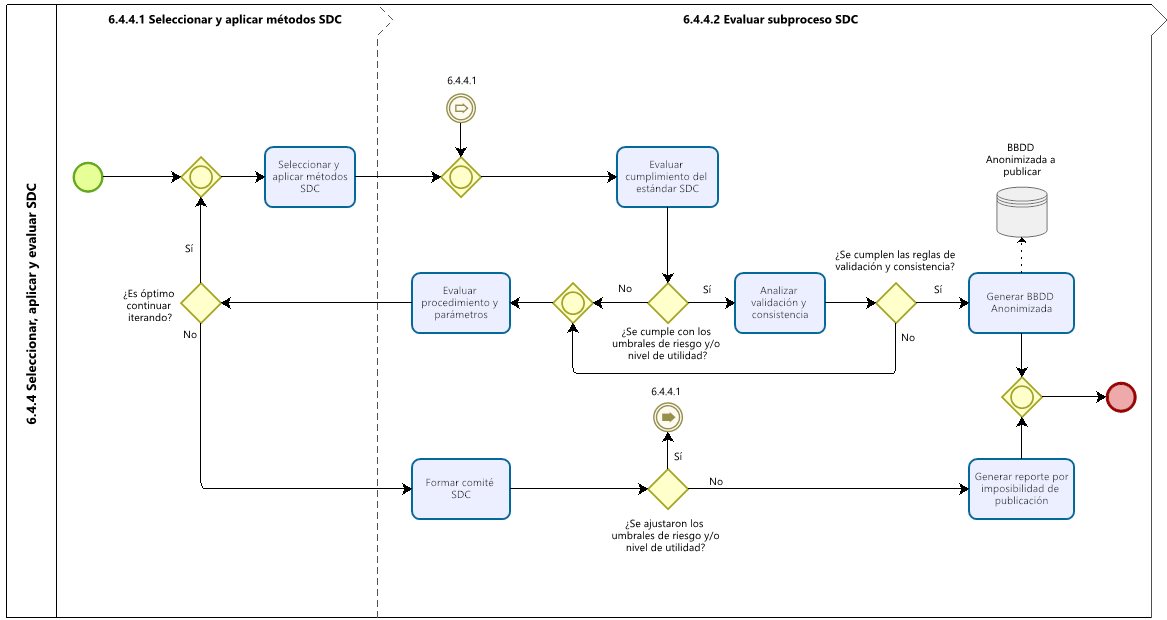
\includegraphics[width=0.9\linewidth]{Imagenes/Eval_Proc_SDC} 

}

\caption{Evaluación de proceso SDC INE 2021.}\label{fig:evalSDC}
\end{figure}

\hypertarget{etapa-6.4.5-generar-reportes-y-liberar-datos}{%
\section{Etapa 6.4.5: Generar reportes y liberar datos}\label{etapa-6.4.5-generar-reportes-y-liberar-datos}}

El propósito de esta etapa es la generación de reportes, tanto interno como externo, que acompañan la liberación de datos.

Los informes internos contienen la descripción exacta de los métodos de anonimización utilizados, los parámetros, pero también las medidas de riesgo antes y después de la anonimización. Esto permite la replicación del conjunto de datos anonimizados y es importante para las autoridades/organismos de control para garantizar que el proceso de anonimización sea suficiente para garantizar el anonimato de acuerdo con la legislación aplicable.

Los informes externos informan al usuario que los datos han sido anonimizados, brindan información para un análisis válido de los datos y explican las limitaciones de los datos como resultado de la anonimización. Puede incluirse una breve descripción de los métodos utilizados. La publicación de microdatos anonimizados debe ir acompañada de los metadatos habituales de la encuesta (peso de la encuesta, estratos, metodología de la encuesta), así como información sobre los métodos de anonimización que permiten a los investigadores realizar análisis válidos (por ejemplo, cantidad de ruido agregado, matriz de transición para PRAM).Se debe tener cuidado de que esta información no se pueda utilizar para la reidentificación (por ejemplo, no se libera semilla aleatoria para PRAM).

Por otra parte, los metadatos deben actualizarse para cumplir con los datos anonimizados. Las descripciones de las variables o las etiquetas de valores pueden haber cambiado como resultado del proceso de anonimización. Además, la pérdida de información debido al proceso de anonimización debe explicarse en detalle a los usuarios para que sean conscientes de los límites de la validez de los datos y sus análisis.

El último paso en el proceso de SDC es la publicación real de los datos anónimos. En el contexto INE, el tipo de publicación factible es el PUF. Los cambios realizados en las variables en la \protect\hyperlink{etapa-6.4.2-preparaciuxf3n-y-exploraciuxf3n-de-datos}{Etapa 6.4.2: Preparación y exploración de datos}, como la fusión de variables, se pueden deshacer para generar un conjunto de datos útil para los usuarios.

\begin{figure}

{\centering 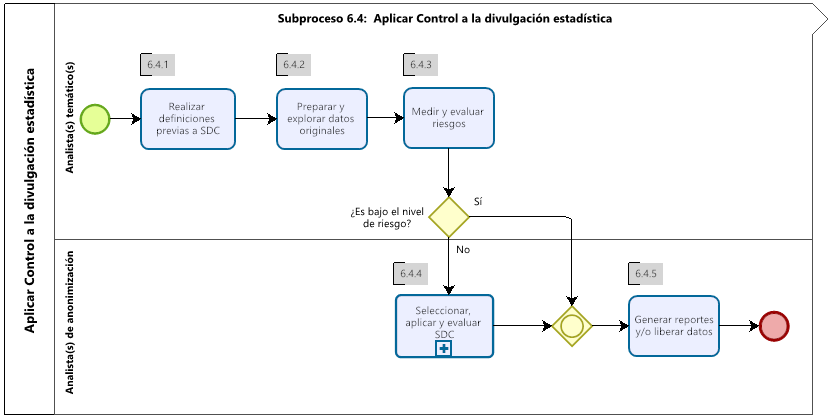
\includegraphics[width=0.9\linewidth]{Imagenes/Esquema_Proc_SDC} 

}

\caption{Esquema general de proceso SDC INE 2021.}\label{fig:esquemaSDC}
\end{figure}

\hypertarget{caso-de-estudio}{%
\chapter{Caso de estudio}\label{caso-de-estudio}}

El objetivo del siguiente proceso de anonimización es ilustrar el proceso SDC establecido en la GUÍA PARA EL CONTROL DE DIVULGACIÓN ESTADÍSTICA EN MICRODATOS propuesta por la Mesa de Anonimización INE. Los datos utilizados corresponden a una base de datos sintética que se basa en el diseño de la 17a ENUSC 2020 \citep{manualbdenusc}.

El proceso SDC aquí implementado pretender generar un archivo de datos PUF (del inglés, \emph{Public Use File}), que pueda ponerse a disposición de forma pública y para cualquier usuario que lo requiera. Para ello, el proceso SDC aplicado apunta al logro de los umbrales de riesgo establecido por la GUÍA PARA EL CONTROL DE DIVULGACIÓN ESTADÍSTICA EN MICRODATOS para encuestas de hogares \citep{manualsdcine}. Simultáneamente, el ejercicio busca mantener la utilidad de los datos, intentando minimizar la intervención de los mismos para que los usuarios puedan replicar las estadísticas priorizadas por esta encuesta.

Los umbrales de riesgo establecidos son los siguientes:

\textbf{RIESGO GLOBAL}

\begin{itemize}
\tightlist
\item
  Riesgo global inferior al 10\%
\end{itemize}

\textbf{RIESGOS INDIVIDUALES}

\begin{itemize}
\tightlist
\item
  Hasta 20\% de observaciones con riesgo individual mayor al 1\%
\item
  Hasta 15\% de observaciones con riesgo individual mayor al 5\%
\item
  0\% de observaciones con riesgo individual mayor al 25\%
\end{itemize}

\textbf{K-ANONIMATO}

\begin{itemize}
\tightlist
\item
  0\% de observaciones violando k = 2
\item
  Hasta 5\% de observaciones violando k = 3
\item
  Hasta 10\% de observaciones violando k = 5
\end{itemize}

A continuación, la guía presenta paso a paso como proceder con este conjunto de datos para lograr el cumplimiento de estos umbrales de riesgo.

\hypertarget{paso-uno-definiciones-previas-al-proceso-de-anonimizaciuxf3n}{%
\section{Paso Uno: Definiciones previas al proceso de anonimización}\label{paso-uno-definiciones-previas-al-proceso-de-anonimizaciuxf3n}}

\hypertarget{definiciuxf3n-del-equipo-de-trabajo}{%
\subsection{Definición del equipo de trabajo}\label{definiciuxf3n-del-equipo-de-trabajo}}

En esta primera etapa, se define el equipo de trabajo, el cual debe estar compuesto al menos por un encargado temático, encargado de los criterios para la selección de variables claves y definición de escenarios, y un analista de anonimización, encargando de la implementación de la misma a través de un \emph{script} como el aquí expuesto.

\hypertarget{insumos-yo-productos-necesarios-para-la-ejecuciuxf3n-del-proceso}{%
\subsection{Insumos y/o productos necesarios para la ejecución del proceso}\label{insumos-yo-productos-necesarios-para-la-ejecuciuxf3n-del-proceso}}

En esta etapa se describe la metodología del producto estadístico, la revisión temática de la base de datos, su caracterización y clasificación de variables, la infraestructura con que se cuenta para el proceso, entre otros elementos que se especifican en el documento adjunto.

\hypertarget{archivo-de-base-de-datos}{%
\subsubsection{Archivo de Base de datos}\label{archivo-de-base-de-datos}}

Antes de cargar los datos, declaramos el directorio de trabajo donde se ubican los archivos con que trabajaremos.

\begin{example}
\protect\hypertarget{exm:bloque1nbm}{}\label{exm:bloque1nbm}Indicar el directorio de trabajo
\end{example}

\begin{Shaded}
\begin{Highlighting}[]
\NormalTok{yourdirectory}\OtherTok{\textless{}{-}}\StringTok{"/simulacion"} 
\FunctionTok{setwd}\NormalTok{(yourdirectory)}
\end{Highlighting}
\end{Shaded}

Se trabaja con la base bruta de la ENUSC, que contiene todas las variables previo a la innominación (en este caso es una base de datos sintética).

\begin{example}
\protect\hypertarget{exm:bloque2nbm}{}\label{exm:bloque2nbm}Indicar el nombre del archivo de datos
\end{example}

\begin{Shaded}
\begin{Highlighting}[]
\NormalTok{fname }\OtherTok{\textless{}{-}} \StringTok{"BD\_ENUSC\_SINTETICA\_ETIQUETADA.sav"}
\NormalTok{file }\OtherTok{\textless{}{-}}\NormalTok{ haven}\SpecialCharTok{::}\FunctionTok{read\_sav}\NormalTok{(fname)}
\end{Highlighting}
\end{Shaded}

\hypertarget{caracterizaciuxf3n-de-la-base-de-datos}{%
\subsubsection{Caracterización de la base de datos}\label{caracterizaciuxf3n-de-la-base-de-datos}}

Primero revisamos las dimensiones del archivo, es decir, cuantos registros y variables contiene. La base contiene 47.344 registros y 73 variables. Luego, revisamos el nombre de las variables contenido en la base de datos para verificar que se ajusta a la base con que se requiere trabajar.

\begin{example}
\protect\hypertarget{exm:bloque3nbm}{}\label{exm:bloque3nbm}Inspeccionar las dimensiones del conjunto de datos y los nombres de las columnas
\end{example}

\begin{Shaded}
\begin{Highlighting}[]
\FunctionTok{dim}\NormalTok{(file)}
\end{Highlighting}
\end{Shaded}

\begin{verbatim}
## [1] 47344    73
\end{verbatim}

\begin{Shaded}
\begin{Highlighting}[]
\FunctionTok{names}\NormalTok{(file)}
\end{Highlighting}
\end{Shaded}

\begin{verbatim}
##  [1] "enc_idr"                  "rph_ID"                  
##  [3] "enc_id"                   "enc_region"              
##  [5] "enc_rpc"                  "enc_distrito"            
##  [7] "enc_zona"                 "enc_manzana"             
##  [9] "enc_vivienda"             "IDC"                     
## [11] "enc_letraKish"            "enc_direccion"           
## [13] "enc_numero"               "enc_codfono"             
## [15] "enc_fono"                 "enc_Nombre_ID"           
## [17] "Enc_Fono_ID"              "Enc_Correo_ID"           
## [19] "enc_Nombre_K"             "enc_Edad_K"              
## [21] "Enc_Fono_K"               "Enc_Correo_K"            
## [23] "FECHA"                    "IH_residencia_habitual"  
## [25] "Hora_inicio_rph"          "rph_numeroLinea"         
## [27] "rph_nombrepila"           "rph_parentesco"          
## [29] "rph_dianacimiento"        "rph_mesnacimiento"       
## [31] "rph_agnonacimiento"       "rph_edad"                
## [33] "rph_sexo"                 "rph_idgen"               
## [35] "Kish"                     "rph_pertenencia_indigena"
## [37] "rph_nacionalidad"         "rph_migracion"           
## [39] "rph_p9"                   "rph_p10"                 
## [41] "rph_p11"                  "rph_p12"                 
## [43] "rph_p13"                  "rph_p14"                 
## [45] "Hora_termino_rph"         "P17"                     
## [47] "P24"                      "A1_1_1"                  
## [49] "A1_1_1_N_Veces"           "B1_1_1"                  
## [51] "B1_1_1_N_Veces"           "C1_1_1"                  
## [53] "C1_1_1_N_Veces"           "D1_1_1"                  
## [55] "D1_1_1_N_Veces"           "E1_1_1"                  
## [57] "E1_1_1_N_Veces"           "F1_1_1"                  
## [59] "G1_1_1"                   "G1_1_1_N_Veces"          
## [61] "H1_1_1"                   "H1_1_1_N_Veces"          
## [63] "VA_DC"                    "VP_DC"                   
## [65] "DEN_AGREG"                "RVA_DC"                  
## [67] "Hora_inicio_cc"           "Hora_termino_cc"         
## [69] "Fact_Pers"                "Fact_Hog"                
## [71] "VarStrat"                 "Conglomerado"            
## [73] "Fact_Ind"
\end{verbatim}

Es importante señalar que la base de datos se compone de variables de caracterización de los hogares y las personas (módulo de Registro de Personas en el Hogar o RPH) y variables temáticas de la encuesta referidas a percepción de inseguridad y victimización.

Adicionalmente, la base de datos contiene pesos muestrales, que deben ser considerados durante la anonimización. Para el nivel hogar se utiliza Fact\_Hog, mientras que para el nivel persona se utiliza Fact\_Ind.

Además, la base de datos cuenta con variables de Conglomerado y VarStrat, que serán utilizadas para declarar el diseño complejo y evaluar la utilidad de los datos antes y después del tratamiento de los mismos.

El archivo ``Diccionario de Variables.xlsx'' contiene la descripción de las variables contenidas en la base de datos.

\hypertarget{clasificaciuxf3n-de-variables-1}{%
\subsubsection{Clasificación de variables}\label{clasificaciuxf3n-de-variables-1}}

Las potenciales variables clave, que podría permitir una re-identificación, se ubican en el módulo de Registro de Personas en el Hogar (RPH), ya que permiten dar cuenta de atributos de las personas y hogares, como también en la portada de la encuesta, donde se encuentran las variables de ubicación geográfica. Estas últimas coinciden en parte con la base de datos de Hoja de Ruta, no obstante esta base no se publica.

\hypertarget{libreruxedas-requeridas}{%
\subsubsection{Librerías requeridas}\label{libreruxedas-requeridas}}

Se cargan las librerías requeridas para el proceso. En caso de que no estén instaladas, deberá instalarlas con la función \texttt{install.packages()} como se muestra en el siguiente ejemplo:

\begin{example}
\protect\hypertarget{exm:bloque4nbm}{}\label{exm:bloque4nbm}Ejemplo de instalación de librería
\end{example}

\begin{Shaded}
\begin{Highlighting}[]
\CommentTok{\#install.packages("nombre\_libreria") }
\end{Highlighting}
\end{Shaded}

Luego, cargamos las librerías:

\begin{example}
\protect\hypertarget{exm:bloque5nbm}{}\label{exm:bloque5nbm}Cargar librerías
\end{example}

\begin{Shaded}
\begin{Highlighting}[]
\FunctionTok{library}\NormalTok{(sdcMicro)  }\CommentTok{\# paquete sdcMicro con funciones para el proceso SDC}
\FunctionTok{library}\NormalTok{(survey)    }\CommentTok{\# para diseño complejo}
\FunctionTok{library}\NormalTok{(calidad)   }\CommentTok{\# evaluación de calidad de las estimaciones}
\FunctionTok{library}\NormalTok{(tidyverse) }\CommentTok{\# herramientas para manipulación de datos}
\FunctionTok{library}\NormalTok{(openxlsx)  }\CommentTok{\# lectura/escritura de archivos xlsx}
\FunctionTok{library}\NormalTok{(stringr) }\CommentTok{\# procesamiento de textos}
\end{Highlighting}
\end{Shaded}

\hypertarget{determinaciuxf3n-de-necesidades-de-protecciuxf3n-de-confidencialidad}{%
\subsection{Determinación de necesidades de protección de confidencialidad}\label{determinaciuxf3n-de-necesidades-de-protecciuxf3n-de-confidencialidad}}

En esta actividad se describen el marco normativo y convenios a tener en cuenta para la anonimización, las unidades estadísticas contenidas en la base de datos, las variables sensibles contenidas en la base de datos, y el diagnóstico de necesidad de protección de confidencialidad.

\hypertarget{unidades-estaduxedsticas}{%
\subsubsection{Unidades estadísticas}\label{unidades-estaduxedsticas}}

Se verifica la cantidad de viviendas y de personas registradas en la base de datos. Para ello, se mide la cantidad de valores únicos del folio de viviendas (\emph{enc\_idr}) y el folio de personas (\emph{rph\_ID}).

\textbf{Viviendas:} 18.766
\textbf{Personas:} 47.344

\begin{example}
\protect\hypertarget{exm:bloque6nbm}{}\label{exm:bloque6nbm}Contar la cantidad de folios a nivel de viviendas y personas
\end{example}

\begin{Shaded}
\begin{Highlighting}[]
\FunctionTok{length}\NormalTok{(}\FunctionTok{unique}\NormalTok{(file}\SpecialCharTok{$}\NormalTok{enc\_idr))}
\end{Highlighting}
\end{Shaded}

\begin{verbatim}
## [1] 18766
\end{verbatim}

\begin{Shaded}
\begin{Highlighting}[]
\FunctionTok{length}\NormalTok{(}\FunctionTok{unique}\NormalTok{(file}\SpecialCharTok{$}\NormalTok{rph\_ID))}
\end{Highlighting}
\end{Shaded}

\begin{verbatim}
## [1] 47344
\end{verbatim}

De este modo, se da cuenta de la cantidad de unidades estadísticas y de la estructura jerárquica de la base de datos.

\hypertarget{variables-sensibles}{%
\subsubsection{variables sensibles}\label{variables-sensibles}}

Se establecen como variables sensibles aquellas referidas a la tenencia de armas (P17), a elementos de seguridad en la vivienda (P24), y acerca de denuncia de delitos (DEN\_AGREG).

\begin{example}
\protect\hypertarget{exm:bloque7nbm}{}\label{exm:bloque7nbm}Guardar variables sensibles en un vector de texto
\end{example}

\begin{Shaded}
\begin{Highlighting}[]
\NormalTok{sensibles }\OtherTok{\textless{}{-}} \FunctionTok{c}\NormalTok{(}\StringTok{\textquotesingle{}P17\textquotesingle{}}\NormalTok{,}
               \StringTok{\textquotesingle{}P24\textquotesingle{}}\NormalTok{,}
               \StringTok{\textquotesingle{}DEN\_AGREG\textquotesingle{}}\NormalTok{)}
\end{Highlighting}
\end{Shaded}

Se verifica que las variables sensibles están presentes en la base de datos. Se espera que esta función devuelva el valor \emph{TRUE}.

\begin{example}
\protect\hypertarget{exm:bloque8nbm}{}\label{exm:bloque8nbm}Verificar presencia de variables sensibles
\end{example}

\begin{Shaded}
\begin{Highlighting}[]
\FunctionTok{all}\NormalTok{(sensibles }\SpecialCharTok{\%in\%} \FunctionTok{names}\NormalTok{(file))}
\end{Highlighting}
\end{Shaded}

\begin{verbatim}
## [1] TRUE
\end{verbatim}

\hypertarget{diagnuxf3stico-de-necesidad-de-protecciuxf3n-de-confidencialidad}{%
\subsubsection{Diagnóstico de necesidad de protección de confidencialidad}\label{diagnuxf3stico-de-necesidad-de-protecciuxf3n-de-confidencialidad}}

Dado que las variables sensibles se encuentran presentes en el archivo de datos, corresponde aplicar el proceso SDC para asegurar la anonimización de los datos.

\hypertarget{propiedades-estaduxedsticas-a-preservar}{%
\subsection{Propiedades estadísticas a preservar}\label{propiedades-estaduxedsticas-a-preservar}}

\hypertarget{usos-claves-de-los-datos}{%
\subsubsection{Usos claves de los datos}\label{usos-claves-de-los-datos}}

Se espera que los datos mantengan las siguientes propiedades:

\begin{itemize}
\item
  Se debe poder reproducir los indicadores principales de la encuesta con precisión, por lo que idealmente no deben modificarse, con un máximo de diferencia en la estimación no mayor a un punto porcentual (diferencia en términos absolutos, dado que las estimaciones de ENUSC son de proporción).
\item
  Además, se deben mantener las variables de desagregación de tabulados de la encuesta, siendo estas sexo y región. Es decir, no deben observarse valores perdidos en estas variables.
\end{itemize}

Dado que las variables temáticas no corresponden a potenciales variables clave, se descuenta la posibilidad de modificar dichas variables, asegurando mantener sus propiedades estadísticas.

Por ende, el foco debe estar en mantener las relaciones entre las variables de desagregación que podrían ser modificadas como sexo y región, y las variables de los indicadores principales.

Un dato frecuentemente solicitado por transparencia es la variable comuna. Si bien el diseño muestral de ENUSC no permite realizar estimaciones a ese nivel de desagregación, esta variable es de todos modos de interés para los usuarios para análisis a nivel descriptivo y referencial. En este sentido, es pertinente evaluar la posibilidad de mantener esta variable en la base de datos anonimizada.

Por otro lado, la variable de edad en versiones anteriores de la ENUSC se publicaba con todos los valores de la variable (semi-continua), siendo ahora publicada como tramos etarios. Dado que usuarios del mundo académico y otros investigadores dan uso a esta variable, es también de interés analizar la posibilidad de mantenerla como semi-continua

\hypertarget{indicadores-priorizados}{%
\subsubsection{Indicadores priorizados}\label{indicadores-priorizados}}

Los indicadores priorizados corresponden a:

\textbf{Victimización Agregada de Delitos Consumados}
Calculado en base a la variable VA\_DC, por lo que la base de datos anonimizada debe permitir calcular este indicador a nivel nacional y regional (corresponde a hogares, por lo que no es desagregable por sexo).

\textbf{Victimización Personal de Delitos Consumados}
Calculado en base a la variable VP\_DC, por lo que la base de datos anonimizada debe permitir calcular este indicador a nivel nacional, regional y según sexo.

Finalmente, dado que la variable de edad es de interés para el análisis de cómo distintos grupos etarios se ven afectados por la delincuencia, es de interés que la relación entre la variable de edad y la variable de victimización personal se mantenga. Esto se evaluará a través de un modelo de regresión logística simple.

\hypertarget{mediciuxf3n-de-utilidad}{%
\subsubsection{Medición de utilidad}\label{mediciuxf3n-de-utilidad}}

\hypertarget{reproducciuxf3n-de-estimaciones-y-desagregaciones}{%
\paragraph{Reproducción de estimaciones y desagregaciones}\label{reproducciuxf3n-de-estimaciones-y-desagregaciones}}

Dado que las variables de sexo, región y de los indicadores principales no serán modificadas se espera que estas mantengan las propiedades estadísticas de la base de datos original o no tratada con la mayor fidelidad posible. Partiendo del supuesto de que estas variables no serán modificadas, sino que el proceso SDC se aplicará sobre otras variables (principalmente otras variables del RPH), solo podría verse alteradas las estimaciones en caso de supresión de registros.

En este sentido, se espera que las estimaciones no difieran de la estimación original en más de un punto porcentual, en tanto diferencia en términos absolutos (todos los indicadores de ENUSC son de proporción).

A continuación, se presentan las estimaciones de la ENUSC utilizando el paquete de calidad de las estimaciones desarrollado en el INE, ya que también se espera que se mantengan los estándares de calidad de las estimaciones.

Ahora, se trabaja con un conjunto que contiene solo a los informantes que respondieron la encuesta (\emph{file\_kish}), descartando al resto de los integrantes del hogar. Esto es un paso necesario para poder declarar el diseño complejo de la encuesta.

Se establece el diseño complejo para personas y para hogares:

\begin{example}
\protect\hypertarget{exm:bloque9nbm}{}\label{exm:bloque9nbm}Declarar el diseño complejo
\end{example}

\begin{Shaded}
\begin{Highlighting}[]
\NormalTok{file\_kish }\OtherTok{\textless{}{-}}\NormalTok{ file[file}\SpecialCharTok{$}\NormalTok{Kish  }\SpecialCharTok{\%in\%} \DecValTok{1}\NormalTok{,]}

\FunctionTok{options}\NormalTok{(}\AttributeTok{survey.lonely.psu =} \StringTok{"certainty"}\NormalTok{)}

\NormalTok{dc\_pers }\OtherTok{\textless{}{-}} \FunctionTok{svydesign}\NormalTok{(}\AttributeTok{ids =} \SpecialCharTok{\textasciitilde{}}\NormalTok{Conglomerado, }
                     \AttributeTok{strata =} \SpecialCharTok{\textasciitilde{}}\NormalTok{VarStrat, }
                     \AttributeTok{data =}\NormalTok{ file\_kish,}
                     \AttributeTok{weights =} \SpecialCharTok{\textasciitilde{}}\NormalTok{Fact\_Pers)}

\NormalTok{dc\_hog }\OtherTok{\textless{}{-}} \FunctionTok{svydesign}\NormalTok{(}\AttributeTok{ids =} \SpecialCharTok{\textasciitilde{}}\NormalTok{Conglomerado, }
                    \AttributeTok{strata =} \SpecialCharTok{\textasciitilde{}}\NormalTok{VarStrat, }
                    \AttributeTok{data =}\NormalTok{ file\_kish,}
                    \AttributeTok{weights =} \SpecialCharTok{\textasciitilde{}}\NormalTok{Fact\_Hog)}
\end{Highlighting}
\end{Shaded}

Luego, realizamos las estimaciones desagregadas por región y sexo, guardando las tablas para posterior evaluación de la utilidad de los datos.

Victimización agregada de delitos consumados, desagregado por región:

\begin{example}
\protect\hypertarget{exm:bloque10nbm}{}\label{exm:bloque10nbm}Estimar Victimización Agregada a nivel regional, con estandar de calidad INE
\end{example}

\begin{Shaded}
\begin{Highlighting}[]
\NormalTok{insumos\_prop }\OtherTok{\textless{}{-}} \FunctionTok{create\_prop}\NormalTok{(}\AttributeTok{var =} \StringTok{\textquotesingle{}VA\_DC\textquotesingle{}}\NormalTok{, }
                                   \AttributeTok{domains =} \StringTok{\textquotesingle{}enc\_region\textquotesingle{}}\NormalTok{, }
                                   \AttributeTok{design =}\NormalTok{  dc\_hog)}

\NormalTok{VA\_DC\_REG\_PRE }\OtherTok{\textless{}{-}} \FunctionTok{assess}\NormalTok{(insumos\_prop)}
\NormalTok{VA\_DC\_REG\_PRE[}\DecValTok{1}\SpecialCharTok{:}\DecValTok{6}\NormalTok{]}
\end{Highlighting}
\end{Shaded}

\begin{verbatim}
##    enc_region      stat         se   df    n         cv
## 1           1 0.5180939 0.01656239 1117 1283 0.03196793
## 2           2 0.4986086 0.02015781  701  834 0.04042813
## 3           3 0.5025207 0.01687235 1048 1224 0.03357544
## 4           4 0.5096128 0.01963187  763  892 0.03852312
## 5           5 0.5046148 0.01265927 1821 2106 0.02508700
## 6           6 0.4937284 0.01719661 1017 1169 0.03483011
## 7           7 0.5193102 0.01797112  920 1067 0.03460576
## 8           8 0.5170244 0.01427234 1474 1724 0.02760477
## 9           9 0.5070849 0.01951509  753  889 0.03848486
## 10         10 0.5261810 0.01672262 1085 1251 0.03178111
## 11         11 0.5240267 0.01849898  903 1066 0.03530160
## 12         12 0.5167737 0.01889486  796  932 0.03656313
## 13         13 0.5084057 0.02151621  604  731 0.04232094
## 14         14 0.5096388 0.01751652  975 1135 0.03437047
## 15         15 0.5026934 0.01590767 1191 1365 0.03164488
## 16         16 0.4899313 0.01751388  929 1098 0.03574763
\end{verbatim}

Victimización personal de delitos consumados, desagregado por sexo:

\begin{example}
\protect\hypertarget{exm:bloque11nbm}{}\label{exm:bloque11nbm}Estimar Victimización Personal según sexo, con estandar de calidad INE
\end{example}

\begin{Shaded}
\begin{Highlighting}[]
\NormalTok{insumos\_prop }\OtherTok{\textless{}{-}} \FunctionTok{create\_prop}\NormalTok{(}\AttributeTok{var =} \StringTok{\textquotesingle{}VP\_DC\textquotesingle{}}\NormalTok{, }
                                   \AttributeTok{domains =} \StringTok{\textquotesingle{}rph\_sexo\textquotesingle{}}\NormalTok{, }
                                   \AttributeTok{design =}\NormalTok{  dc\_pers}
\NormalTok{                                )}

\NormalTok{VP\_DC\_SEXO\_PRE }\OtherTok{\textless{}{-}} \FunctionTok{assess}\NormalTok{(insumos\_prop)}
\NormalTok{VP\_DC\_SEXO\_PRE[}\DecValTok{1}\SpecialCharTok{:}\DecValTok{6}\NormalTok{]}
\end{Highlighting}
\end{Shaded}

\begin{verbatim}
##   rph_sexo      stat          se   df    n         cv
## 1        1 0.2526373 0.005327597 6721 9439 0.02108793
## 2        2 0.2447268 0.005269227 6590 9327 0.02153106
\end{verbatim}

Victimización personal de delitos consumados, desagregado por región:

\begin{example}
\protect\hypertarget{exm:bloque12nbm}{}\label{exm:bloque12nbm}Estimar Victimización Personal a nivel regional, con estandar de calidad INE
\end{example}

\begin{Shaded}
\begin{Highlighting}[]
\NormalTok{insumos\_prop }\OtherTok{\textless{}{-}} \FunctionTok{create\_prop}\NormalTok{(}\AttributeTok{var =} \StringTok{\textquotesingle{}VP\_DC\textquotesingle{}}\NormalTok{, }
                                   \AttributeTok{domains =} \StringTok{\textquotesingle{}enc\_region\textquotesingle{}}\NormalTok{, }
                                   \AttributeTok{design =}\NormalTok{  dc\_pers)}

\NormalTok{VP\_DC\_REG\_PRE }\OtherTok{\textless{}{-}} \FunctionTok{assess}\NormalTok{(insumos\_prop)}
\NormalTok{VP\_DC\_REG\_PRE[}\DecValTok{1}\SpecialCharTok{:}\DecValTok{6}\NormalTok{]}
\end{Highlighting}
\end{Shaded}

\begin{verbatim}
##    enc_region      stat         se   df    n         cv
## 1           1 0.2568172 0.01420410 1117 1283 0.05530824
## 2           2 0.2313854 0.01700058  701  834 0.07347300
## 3           3 0.2379758 0.01447234 1048 1224 0.06081436
## 4           4 0.2475154 0.01704076  763  892 0.06884725
## 5           5 0.2422258 0.01087581 1821 2106 0.04489945
## 6           6 0.2521763 0.01503618 1017 1169 0.05962565
## 7           7 0.2685464 0.01612499  920 1067 0.06004546
## 8           8 0.2611829 0.01250193 1474 1724 0.04786657
## 9           9 0.2412502 0.01739434  753  889 0.07210085
## 10         10 0.2361271 0.01413669 1085 1251 0.05986900
## 11         11 0.2773473 0.01612302  903 1066 0.05813297
## 12         12 0.2396374 0.01618739  796  932 0.06754952
## 13         13 0.2462710 0.01884833  604  731 0.07653493
## 14         14 0.2527983 0.01529804  975 1135 0.06051481
## 15         15 0.2404411 0.01327941 1191 1365 0.05522937
## 16         16 0.2431671 0.01512454  929 1098 0.06219815
\end{verbatim}

Victimización personal de delitos consumados, desagregado por sexo y región:

\begin{example}
\protect\hypertarget{exm:bloque13nbm}{}\label{exm:bloque13nbm}Estimar Victimización Personal a nivel regional y según sexo, con estandar de calidad INE
\end{example}

\begin{Shaded}
\begin{Highlighting}[]
\NormalTok{insumos\_prop }\OtherTok{\textless{}{-}} \FunctionTok{create\_prop}\NormalTok{(}\AttributeTok{var =} \StringTok{\textquotesingle{}VP\_DC\textquotesingle{}}\NormalTok{, }
                                   \AttributeTok{domains =} \StringTok{\textquotesingle{}rph\_sexo+enc\_region\textquotesingle{}}\NormalTok{, }
                                   \AttributeTok{design =}\NormalTok{  dc\_pers)}

\NormalTok{VP\_DC\_REG\_SEXO\_PRE }\OtherTok{\textless{}{-}} \FunctionTok{assess}\NormalTok{(insumos\_prop)}
\NormalTok{VP\_DC\_REG\_SEXO\_PRE[}\DecValTok{1}\SpecialCharTok{:}\DecValTok{6}\NormalTok{]}
\end{Highlighting}
\end{Shaded}

\begin{verbatim}
##    rph_sexo enc_region      stat         se  df    n
## 1         1          1 0.2612492 0.01993875 541  660
## 2         2          1 0.2522270 0.02020040 508  623
## 3         1          2 0.2138315 0.02274576 317  428
## 4         2          2 0.2493531 0.02527904 304  406
## 5         1          3 0.2392046 0.02068420 485  600
## 6         2          3 0.2367133 0.02041682 501  624
## 7         1          4 0.2571475 0.02439808 340  440
## 8         2          4 0.2388935 0.02367246 342  452
## 9         1          5 0.2582590 0.01563089 921 1067
## 10        2          5 0.2261775 0.01500918 889 1039
## 11        1          6 0.2557568 0.02147664 472  582
## 12        2          6 0.2486357 0.02088754 469  587
## 13        1          7 0.2751938 0.02324332 429  540
## 14        2          7 0.2616656 0.02226621 412  527
## 15        1          8 0.2826785 0.01822327 688  829
## 16        2          8 0.2408143 0.01715973 746  895
## 17        1          9 0.2479841 0.02381286 359  467
## 18        2          9 0.2333432 0.02543398 316  422
## 19        1         10 0.2458082 0.01995371 521  639
## 20        2         10 0.2262334 0.01988504 492  612
## 21        1         11 0.2660547 0.02254731 422  531
## 22        2         11 0.2894683 0.02341303 418  535
## 23        1         12 0.2383125 0.02254203 365  475
## 24        2         12 0.2410698 0.02307637 352  457
## 25        1         13 0.2515748 0.02693269 252  356
## 26        2         13 0.2411737 0.02646547 273  375
## 27        1         14 0.2533536 0.02087620 490  598
## 28        2         14 0.2521585 0.02282616 414  537
## 29        1         15 0.2408291 0.01870310 565  686
## 30        2         15 0.2400561 0.01891161 562  679
## 31        1         16 0.2262722 0.02063687 425  541
## 32        2         16 0.2592696 0.02167361 442  557
\end{verbatim}

Se espera que la base de datos anonimizada mantenga las propiedades aquí expuestas, por lo que se almacenan en objetos para su posterior comparación con los datos tratados.

Por otro lado, dado que queremos mantener la utilidad de los datos en relación con edad, se mide la relación entre la variable edad y la variable VP\_DC, lo cual se debería mantener en caso que se deba recodificar la edad en tramos.

\hypertarget{relaciuxf3n-entre-variable-de-edad-y-victimizaciuxf3n-personal}{%
\paragraph{Relación entre variable de edad y victimización personal}\label{relaciuxf3n-entre-variable-de-edad-y-victimizaciuxf3n-personal}}

Se genera un modelo \emph{logit} con la variable de Victimización Personal como dependiente y con la variable de edad como regresor. Se espera que los resultados aquí obtenidos sean similares con los datos tratados, lo que se evaluará al final del proceso de anonimización.

\textbf{Carga de datos}

Primero, se cargan los datos, y se filtran dejando solo al informante Kish.

\begin{example}
\protect\hypertarget{exm:bloque14nbm}{}\label{exm:bloque14nbm}Generar dataframe para modelo
\end{example}

\begin{Shaded}
\begin{Highlighting}[]
\NormalTok{data }\OtherTok{\textless{}{-}}\NormalTok{ file[file}\SpecialCharTok{$}\NormalTok{Kish }\SpecialCharTok{\%in\%} \DecValTok{1}\NormalTok{,]}
\end{Highlighting}
\end{Shaded}

\textbf{Dividir datos en \emph{training} y \emph{testing} sets}

Luego, se dividen los datos en sets de training y testing.

\begin{example}
\protect\hypertarget{exm:bloque15nbm}{}\label{exm:bloque15nbm}Dividir datos en \emph{training} y \emph{testing} sets
\end{example}

\begin{Shaded}
\begin{Highlighting}[]
\FunctionTok{library}\NormalTok{(caTools)}
\FunctionTok{set.seed}\NormalTok{(}\DecValTok{2022}\NormalTok{)}

\NormalTok{ids\_train }\OtherTok{\textless{}{-}} \FunctionTok{sample}\NormalTok{(data}\SpecialCharTok{$}\NormalTok{rph\_ID, }\FunctionTok{nrow}\NormalTok{(data)}\SpecialCharTok{/}\DecValTok{3}\SpecialCharTok{*}\DecValTok{2}\NormalTok{)}
\NormalTok{training}\OtherTok{\textless{}{-}}\NormalTok{ sjlabelled}\SpecialCharTok{::}\FunctionTok{remove\_all\_labels}\NormalTok{(data[data}\SpecialCharTok{$}\NormalTok{rph\_ID }\SpecialCharTok{\%in\%}\NormalTok{ ids\_train,])}
\NormalTok{testing}\OtherTok{\textless{}{-}}\NormalTok{ sjlabelled}\SpecialCharTok{::}\FunctionTok{remove\_all\_labels}\NormalTok{(data[}\SpecialCharTok{!}\NormalTok{data}\SpecialCharTok{$}\NormalTok{rph\_ID }\SpecialCharTok{\%in\%}\NormalTok{ ids\_train,])}
\end{Highlighting}
\end{Shaded}

\textbf{Construir modelo}

Luego, construimos el modelo utilizando la función \texttt{glm()}.

\begin{example}
\protect\hypertarget{exm:bloque16nbm}{}\label{exm:bloque16nbm}Construir modelo
\end{example}

\begin{Shaded}
\begin{Highlighting}[]
\NormalTok{modelo}\OtherTok{\textless{}{-}}\FunctionTok{glm}\NormalTok{(VP\_DC}\SpecialCharTok{\textasciitilde{}}\NormalTok{rph\_edad, }
            \AttributeTok{data=}\NormalTok{training, }
            \AttributeTok{family =} \StringTok{"binomial"}\NormalTok{)}
\FunctionTok{summary}\NormalTok{(modelo)}
\end{Highlighting}
\end{Shaded}

\begin{verbatim}
## 
## Call:
## glm(formula = VP_DC ~ rph_edad, family = "binomial", data = training)
## 
## Deviance Residuals: 
##     Min       1Q   Median       3Q      Max  
## -0.8025  -0.7661  -0.7320  -0.6980   1.7502  
## 
## Coefficients:
##               Estimate Std. Error z value Pr(>|z|)    
## (Intercept) -1.3401916  0.0525124  -25.52  < 2e-16 ***
## rph_edad     0.0034786  0.0007714    4.51  6.5e-06 ***
## ---
## Signif. codes:  0 '***' 0.001 '**' 0.01 '*' 0.05 '.' 0.1 ' ' 1
## 
## (Dispersion parameter for binomial family taken to be 1)
## 
##     Null deviance: 13933  on 12509  degrees of freedom
## Residual deviance: 13912  on 12508  degrees of freedom
## AIC: 13916
## 
## Number of Fisher Scoring iterations: 4
\end{verbatim}

\textbf{Validación de modelo}

Luego aplicamos el test de Hosmer Lemeshow para validar el modelo.

\begin{example}
\protect\hypertarget{exm:bloque17nbm}{}\label{exm:bloque17nbm}Validación de modelo
\end{example}

\begin{Shaded}
\begin{Highlighting}[]
\FunctionTok{library}\NormalTok{(ResourceSelection)}
\end{Highlighting}
\end{Shaded}

\begin{verbatim}
## ResourceSelection 0.3-6   2023-06-27
\end{verbatim}

\begin{Shaded}
\begin{Highlighting}[]
\FunctionTok{hoslem.test}\NormalTok{(modelo}\SpecialCharTok{$}\NormalTok{y,}\FunctionTok{fitted}\NormalTok{(modelo),}\AttributeTok{g=}\DecValTok{10}\NormalTok{) }\CommentTok{\# Test de Hosmer Lemeshow}
\end{Highlighting}
\end{Shaded}

\begin{verbatim}
## 
##  Hosmer and Lemeshow goodness of fit (GOF) test
## 
## data:  modelo$y, fitted(modelo)
## X-squared = 255.13, df = 8, p-value < 2.2e-16
\end{verbatim}

\begin{Shaded}
\begin{Highlighting}[]
\FunctionTok{library}\NormalTok{(pROC)}
\end{Highlighting}
\end{Shaded}

\begin{verbatim}
## Type 'citation("pROC")' for a citation.
\end{verbatim}

\begin{verbatim}
## 
## Attaching package: 'pROC'
\end{verbatim}

\begin{verbatim}
## The following objects are masked from 'package:stats':
## 
##     cov, smooth, var
\end{verbatim}

\begin{Shaded}
\begin{Highlighting}[]
\NormalTok{indiceC.trainig}\OtherTok{\textless{}{-}}\FunctionTok{roc}\NormalTok{(modelo}\SpecialCharTok{$}\NormalTok{y,}\FunctionTok{fitted}\NormalTok{(modelo))     }\CommentTok{\# Curva ROC}
\end{Highlighting}
\end{Shaded}

\begin{verbatim}
## Setting levels: control = 0, case = 1
\end{verbatim}

\begin{verbatim}
## Setting direction: controls < cases
\end{verbatim}

\begin{Shaded}
\begin{Highlighting}[]
\NormalTok{indiceC.trainig}
\end{Highlighting}
\end{Shaded}

\begin{verbatim}
## 
## Call:
## roc.default(response = modelo$y, predictor = fitted(modelo))
## 
## Data: fitted(modelo) in 9444 controls (modelo$y 0) < 3066 cases (modelo$y 1).
## Area under the curve: 0.5272
\end{verbatim}

\textbf{Punto de corte óptimo}

Se calcula el punto de corte óptimo utilizando la función \texttt{coords()}.

\begin{example}
\protect\hypertarget{exm:bloque18nbm}{}\label{exm:bloque18nbm}Calcular punto de corte óptimo
\end{example}

\begin{Shaded}
\begin{Highlighting}[]
\NormalTok{ptocorteop.training}\OtherTok{\textless{}{-}}\FunctionTok{coords}\NormalTok{(indiceC.trainig,}\AttributeTok{x=}\StringTok{"best"}\NormalTok{,}
                            \AttributeTok{input=}\StringTok{"threshold"}\NormalTok{,}
                            \AttributeTok{best.method=}\StringTok{"youden"}\NormalTok{)}
\NormalTok{ptocorteop.training}
\end{Highlighting}
\end{Shaded}

\begin{verbatim}
##   threshold specificity sensitivity
## 1  0.270795   0.9431385   0.1457926
\end{verbatim}

\begin{Shaded}
\begin{Highlighting}[]
\FunctionTok{library}\NormalTok{(ROCR)}
\NormalTok{ROC.training}\OtherTok{\textless{}{-}}\FunctionTok{performance}\NormalTok{(}\AttributeTok{prediction.obj =} \FunctionTok{prediction}\NormalTok{(}\AttributeTok{predictions =} \FunctionTok{fitted}\NormalTok{(modelo),}
                                                      \AttributeTok{labels =} \FunctionTok{as.factor}\NormalTok{(modelo}\SpecialCharTok{$}\NormalTok{y)),}
                          \StringTok{"tpr"}\NormalTok{,}
                          \StringTok{"fpr"}\NormalTok{)}
\end{Highlighting}
\end{Shaded}

Luego, visualizamos el punto de corte óptimo utilizando la función \texttt{plot()}.

\begin{example}
\protect\hypertarget{exm:bloque19nbm}{}\label{exm:bloque19nbm}Visualizar punto de corte óptimo
\end{example}

\begin{Shaded}
\begin{Highlighting}[]
\FunctionTok{plot}\NormalTok{(ROC.training, }\AttributeTok{colorize=}\ConstantTok{TRUE}\NormalTok{, }\AttributeTok{print.cutoffs.at=}\FunctionTok{seq}\NormalTok{(}\FloatTok{0.1}\NormalTok{, }\AttributeTok{by=}\FloatTok{0.1}\NormalTok{))}
\FunctionTok{abline}\NormalTok{(}\AttributeTok{a=}\DecValTok{0}\NormalTok{,}\AttributeTok{b=}\DecValTok{1}\NormalTok{)}
\FunctionTok{abline}\NormalTok{(}\AttributeTok{v=}\NormalTok{ptocorteop.training}\SpecialCharTok{$}\NormalTok{threshold,}\AttributeTok{col=}\StringTok{"red"}\NormalTok{)}
\end{Highlighting}
\end{Shaded}

\begin{figure}
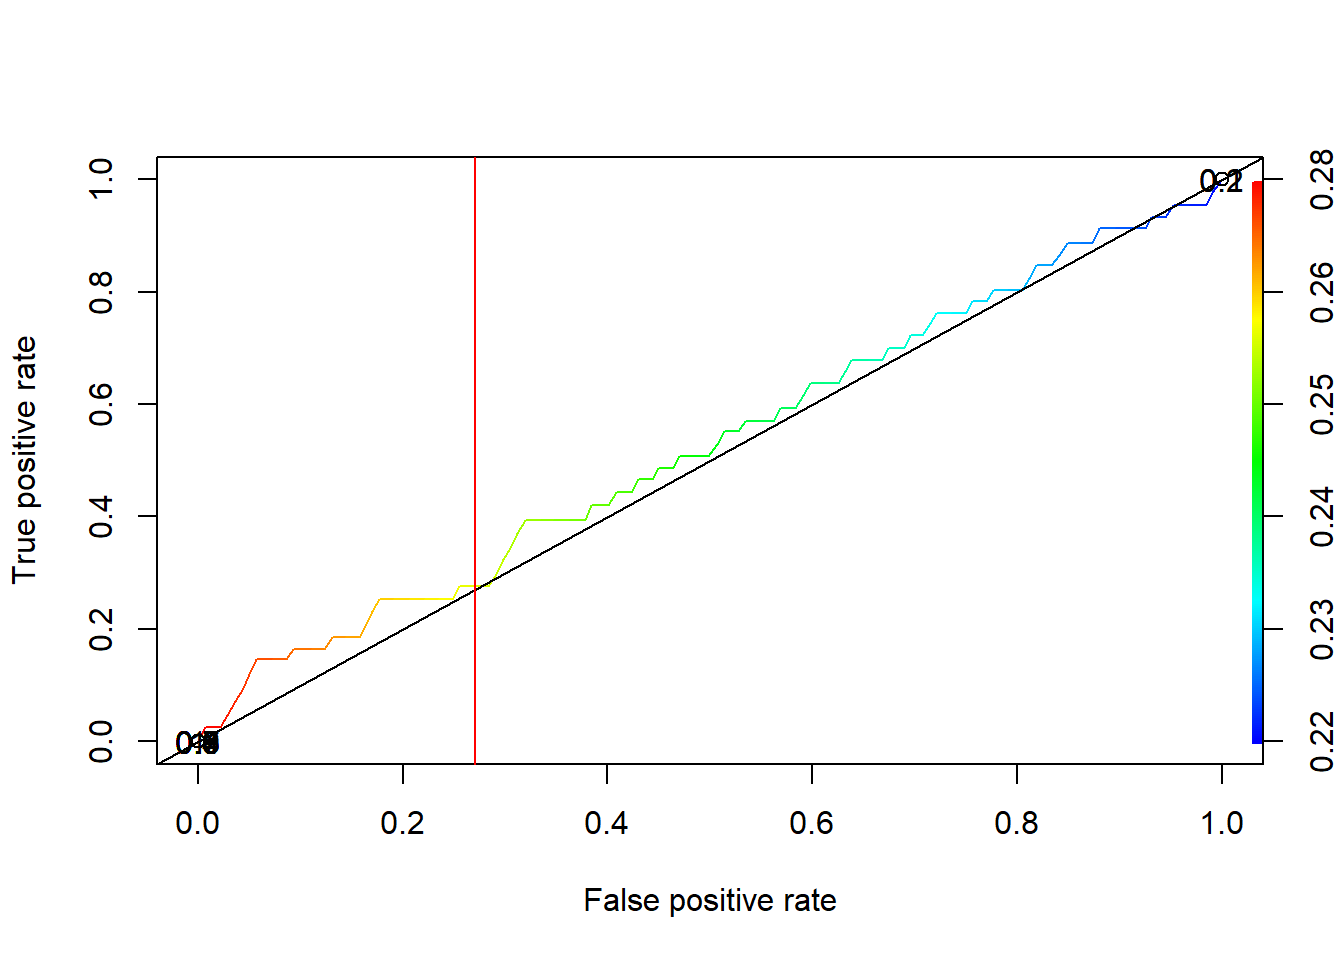
\includegraphics[width=0.9\linewidth]{bookdown-demo_files/figure-latex/unnamed-chunk-92-1} \caption{Punto de corte óptimo con datos no tratados}\label{fig:unnamed-chunk-92}
\end{figure}

\textbf{Predicciones y matriz de confusión}

Se realizan predicciones y se genera una matriz de confusión.

\begin{example}
\protect\hypertarget{exm:bloque20nbm}{}\label{exm:bloque20nbm}Predicciones y matriz de confusión
\end{example}

\begin{Shaded}
\begin{Highlighting}[]
\NormalTok{pred.training}\OtherTok{\textless{}{-}}\FunctionTok{predict}\NormalTok{(modelo, }\AttributeTok{data=}\NormalTok{training, }\AttributeTok{type=}\StringTok{"response"}\NormalTok{)}
\FunctionTok{table}\NormalTok{(}\AttributeTok{ActualValue=}\NormalTok{training}\SpecialCharTok{$}\NormalTok{VP\_DC, }
      \AttributeTok{PredictValue=}\NormalTok{pred.training}\SpecialCharTok{\textgreater{}}\NormalTok{ptocorteop.training}\SpecialCharTok{$}\NormalTok{threshold)}
\end{Highlighting}
\end{Shaded}

\begin{verbatim}
##            PredictValue
## ActualValue FALSE TRUE
##           0  8907  537
##           1  2619  447
\end{verbatim}

A continuación, se continua la evaluación del modelo con datos de prueba.

\textbf{Validación de modelo (con datos de prueba)}

Aplicamos nuevamente la validación con el test de Hosmer Lemeshow, esta vez con los datos de prueba.

\begin{example}
\protect\hypertarget{exm:bloque21nbm}{}\label{exm:bloque21nbm}Validación de modelo con datos de prueba
\end{example}

\begin{Shaded}
\begin{Highlighting}[]
\FunctionTok{hoslem.test}\NormalTok{(testing}\SpecialCharTok{$}\NormalTok{VP\_DC,}\FunctionTok{predict}\NormalTok{(modelo,}\AttributeTok{newdata=}\NormalTok{testing,}\AttributeTok{type=}\StringTok{"response"}\NormalTok{),}\AttributeTok{g=}\DecValTok{5}\NormalTok{)   }\CommentTok{\# Test de Hosmer Lemeshow}
\end{Highlighting}
\end{Shaded}

\begin{verbatim}
## 
##  Hosmer and Lemeshow goodness of fit (GOF) test
## 
## data:  testing$VP_DC, predict(modelo, newdata = testing, type = "response")
## X-squared = 60.369, df = 3, p-value = 4.903e-13
\end{verbatim}

\begin{Shaded}
\begin{Highlighting}[]
\NormalTok{indiceC.testing}\OtherTok{=}\FunctionTok{roc}\NormalTok{(testing}\SpecialCharTok{$}\NormalTok{VP\_DC,}\FunctionTok{predict}\NormalTok{(modelo,}\AttributeTok{newdata=}\NormalTok{testing,}\AttributeTok{type=}\StringTok{"response"}\NormalTok{)) }\CommentTok{\# Curva ROC}
\end{Highlighting}
\end{Shaded}

\begin{verbatim}
## Setting levels: control = 0, case = 1
\end{verbatim}

\begin{verbatim}
## Setting direction: controls < cases
\end{verbatim}

\begin{Shaded}
\begin{Highlighting}[]
\NormalTok{indiceC.testing}
\end{Highlighting}
\end{Shaded}

\begin{verbatim}
## 
## Call:
## roc.default(response = testing$VP_DC, predictor = predict(modelo,     newdata = testing, type = "response"))
## 
## Data: predict(modelo, newdata = testing, type = "response") in 4666 controls (testing$VP_DC 0) < 1590 cases (testing$VP_DC 1).
## Area under the curve: 0.5203
\end{verbatim}

\textbf{Punto de corte óptimo (con datos de prueba)}

Se calcula el punto de corte óptimo utilizando la función \texttt{coords()}.

\begin{example}
\protect\hypertarget{exm:bloque22nbm}{}\label{exm:bloque22nbm}Calcular de corte óptimo con datos de prueba
\end{example}

\begin{Shaded}
\begin{Highlighting}[]
\NormalTok{ptocorteop.testing}\OtherTok{\textless{}{-}}\FunctionTok{coords}\NormalTok{(indiceC.testing,}\AttributeTok{x=}\StringTok{"best"}\NormalTok{,}\AttributeTok{input=}\StringTok{"threshold"}\NormalTok{,}\AttributeTok{best.method=}\StringTok{"youden"}\NormalTok{)}
\NormalTok{ptocorteop.testing}
\end{Highlighting}
\end{Shaded}

\begin{verbatim}
##   threshold specificity sensitivity
## 1 0.2633057   0.8317617   0.2440252
\end{verbatim}

\begin{Shaded}
\begin{Highlighting}[]
\NormalTok{ROC.testing}\OtherTok{\textless{}{-}}\FunctionTok{performance}\NormalTok{(}\FunctionTok{prediction}\NormalTok{(}\FunctionTok{predict}\NormalTok{(modelo,}\AttributeTok{newdata=}\NormalTok{testing,}\AttributeTok{type=}\StringTok{"response"}\NormalTok{),}
                                    \FunctionTok{as.factor}\NormalTok{(testing}\SpecialCharTok{$}\NormalTok{VP\_DC)),}\StringTok{"tpr"}\NormalTok{,}\StringTok{"fpr"}\NormalTok{)}
\end{Highlighting}
\end{Shaded}

Luego, visualizamos el punto de corte óptimo utilizando la función \texttt{plot()}.

\begin{example}
\protect\hypertarget{exm:bloque23nbm}{}\label{exm:bloque23nbm}Visualizar de corte óptimo con datos de prueba
\end{example}

\begin{Shaded}
\begin{Highlighting}[]
\FunctionTok{plot}\NormalTok{(ROC.testing, }\AttributeTok{colorize=}\ConstantTok{TRUE}\NormalTok{, }\AttributeTok{print.cutoffs.at=}\FunctionTok{seq}\NormalTok{(}\FloatTok{0.1}\NormalTok{, }\AttributeTok{by=}\FloatTok{0.1}\NormalTok{))}
\FunctionTok{abline}\NormalTok{(}\AttributeTok{a=}\DecValTok{0}\NormalTok{,}\AttributeTok{b=}\DecValTok{1}\NormalTok{)}
\FunctionTok{abline}\NormalTok{(}\AttributeTok{v=}\NormalTok{ptocorteop.testing}\SpecialCharTok{$}\NormalTok{threshold,}\AttributeTok{col=}\StringTok{"red"}\NormalTok{)}
\end{Highlighting}
\end{Shaded}

\begin{figure}
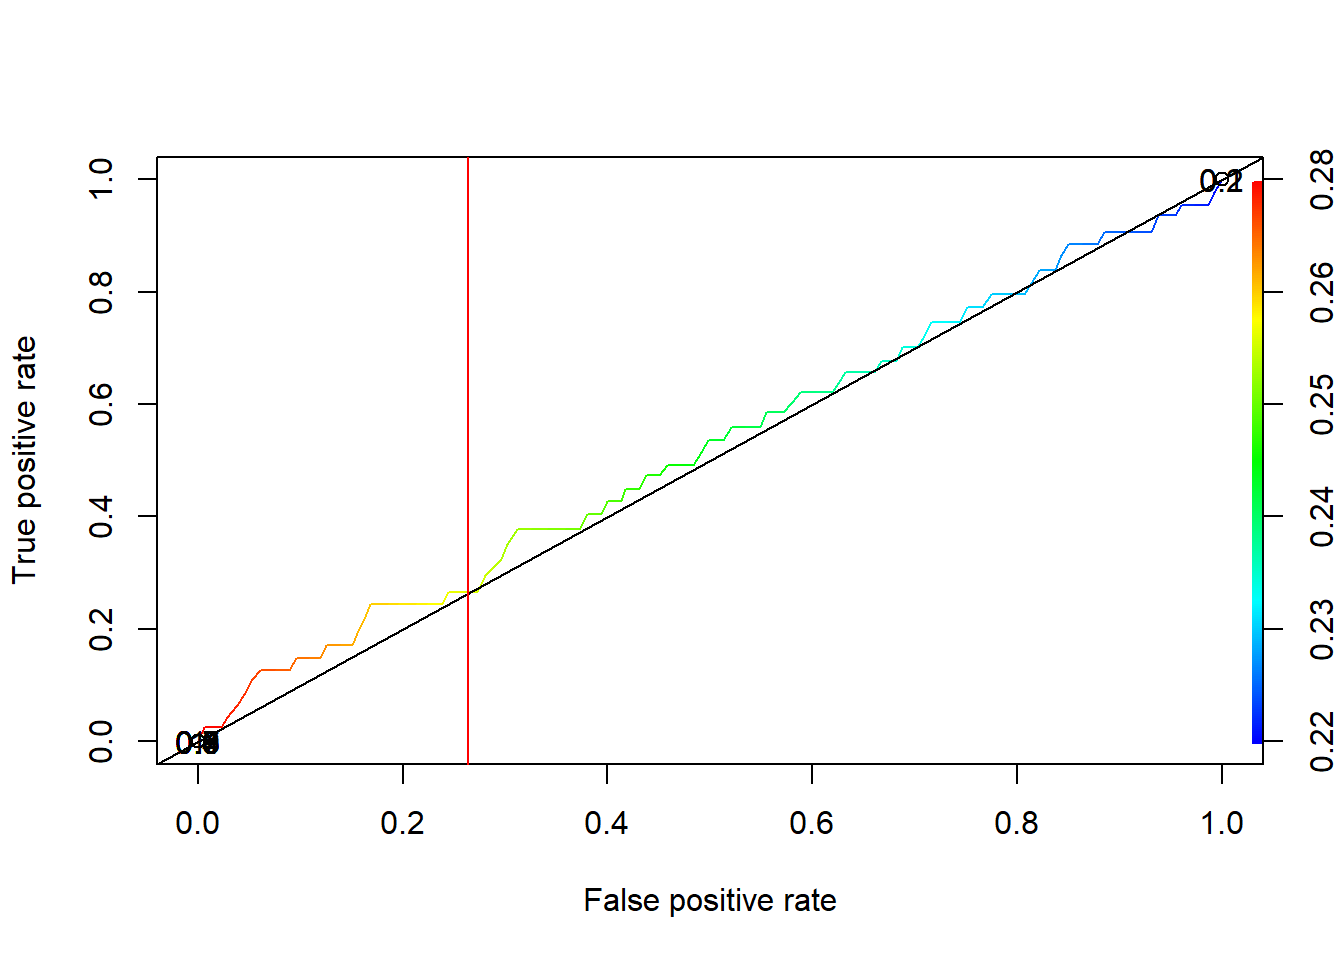
\includegraphics[width=0.9\linewidth]{bookdown-demo_files/figure-latex/unnamed-chunk-96-1} \caption{Punto de corte óptimo con datos de prueba a partir de datos no tratados}\label{fig:unnamed-chunk-96}
\end{figure}

\textbf{Predicciones y matriz de confusión (con datos de prueba)}

Se realizan predicciones y se genera una matriz de confusión.

\begin{example}
\protect\hypertarget{exm:bloque24nbm}{}\label{exm:bloque24nbm}Predicciones y matriz de confusión con datos de prueba
\end{example}

\begin{Shaded}
\begin{Highlighting}[]
\NormalTok{pred.testing}\OtherTok{\textless{}{-}}\FunctionTok{predict}\NormalTok{(modelo, testing, }\AttributeTok{type=}\StringTok{"response"}\NormalTok{)}
\FunctionTok{table}\NormalTok{(}\AttributeTok{ActualValue=}\NormalTok{testing}\SpecialCharTok{$}\NormalTok{VP\_DC, }\AttributeTok{PredictValue=}\NormalTok{pred.testing}\SpecialCharTok{\textgreater{}}\NormalTok{ptocorteop.testing}\SpecialCharTok{$}\NormalTok{threshold)}
\end{Highlighting}
\end{Shaded}

\begin{verbatim}
##            PredictValue
## ActualValue FALSE TRUE
##           0  3881  785
##           1  1202  388
\end{verbatim}

\textbf{Comparar área bajo la curva, umbral, sensibilidad y especificidad}

Finalmente, comparamos el área bajo la curva, umbral, sensibilidad y especificidad, a partir de los resultados del modelo con los datos de entrenamiento y con los datos de prueba.

\begin{example}
\protect\hypertarget{exm:bloque25nbm}{}\label{exm:bloque25nbm}Comparar área bajo la curva, umbral, sensibilidad y especificidad
\end{example}

\begin{Shaded}
\begin{Highlighting}[]
\NormalTok{auc    }\OtherTok{\textless{}{-}}\NormalTok{indiceC.trainig}\SpecialCharTok{$}\NormalTok{auc              }\SpecialCharTok{{-}}\NormalTok{ indiceC.testing}\SpecialCharTok{$}\NormalTok{auc}
\NormalTok{corte  }\OtherTok{\textless{}{-}}\NormalTok{ptocorteop.training}\SpecialCharTok{$}\NormalTok{threshold    }\SpecialCharTok{{-}}\NormalTok{ ptocorteop.testing}\SpecialCharTok{$}\NormalTok{threshold}
\NormalTok{sens   }\OtherTok{\textless{}{-}}\NormalTok{ ptocorteop.training}\SpecialCharTok{$}\NormalTok{sensitivity }\SpecialCharTok{{-}}\NormalTok{ ptocorteop.testing}\SpecialCharTok{$}\NormalTok{sensitivity}
\NormalTok{spe    }\OtherTok{\textless{}{-}}\NormalTok{ ptocorteop.training}\SpecialCharTok{$}\NormalTok{specificity }\SpecialCharTok{{-}}\NormalTok{ ptocorteop.testing}\SpecialCharTok{$}\NormalTok{specificity}
\end{Highlighting}
\end{Shaded}

\hypertarget{paso-dos-preparar-y-explorar-datos-originales}{%
\section{Paso Dos: Preparar y explorar datos originales}\label{paso-dos-preparar-y-explorar-datos-originales}}

\hypertarget{preparaciuxf3n-de-datos}{%
\subsection{Preparación de datos}\label{preparaciuxf3n-de-datos}}

\hypertarget{integraciuxf3n-de-datos}{%
\subsubsection{Integración de datos}\label{integraciuxf3n-de-datos}}

La base de datos ENUSC ya se encuentra integrada y no se combina con ninguna otra base producida para este producto estadístico.

\hypertarget{eliminaciuxf3n-de-identificadores-directos}{%
\subsubsection{Eliminación de identificadores directos}\label{eliminaciuxf3n-de-identificadores-directos}}

Se registra nombres de identificadores directos y otras variables internas del proyecto que no son publicadas.

\begin{example}
\protect\hypertarget{exm:bloque26nbm}{}\label{exm:bloque26nbm}Almacenar indicadores directos y otras variables excluidas en un vector de texto
\end{example}

\begin{Shaded}
\begin{Highlighting}[]
\NormalTok{identificadores\_directos }\OtherTok{\textless{}{-}} \FunctionTok{c}\NormalTok{(}\StringTok{\textquotesingle{}enc\_id\textquotesingle{}}\NormalTok{,}\StringTok{\textquotesingle{}enc\_distrito\textquotesingle{}}\NormalTok{,}
                              \StringTok{\textquotesingle{}enc\_zona\textquotesingle{}}\NormalTok{,}\StringTok{\textquotesingle{}enc\_manzana\textquotesingle{}}\NormalTok{,}\StringTok{\textquotesingle{}enc\_vivienda\textquotesingle{}}\NormalTok{,}\StringTok{\textquotesingle{}FECHA\textquotesingle{}}\NormalTok{,}
                              \StringTok{\textquotesingle{}enc\_Nombre\_ID\textquotesingle{}}\NormalTok{,}
                              \StringTok{\textquotesingle{}enc\_Nombre\_K\textquotesingle{}}\NormalTok{,}\StringTok{\textquotesingle{}enc\_Edad\_K\textquotesingle{}}\NormalTok{,}
                              \StringTok{\textquotesingle{}rph\_dianacimiento\textquotesingle{}}\NormalTok{,}\StringTok{\textquotesingle{}rph\_mesnacimiento\textquotesingle{}}\NormalTok{,}
                              \StringTok{\textquotesingle{}rph\_agnonacimiento\textquotesingle{}}\NormalTok{,}
                              \StringTok{\textquotesingle{}rph\_nombrepila\textquotesingle{}}\NormalTok{,}\StringTok{\textquotesingle{}Hora\_inicio\_rph\textquotesingle{}}\NormalTok{,}
                              \StringTok{\textquotesingle{}Hora\_termino\_rph\textquotesingle{}}\NormalTok{,}\StringTok{\textquotesingle{}Hora\_inicio\_cc\textquotesingle{}}\NormalTok{,}\StringTok{\textquotesingle{}Hora\_termino\_cc\textquotesingle{}}\NormalTok{,}
                              \StringTok{\textquotesingle{}IDC\textquotesingle{}}\NormalTok{,}\StringTok{\textquotesingle{}enc\_letraKish\textquotesingle{}}\NormalTok{,}
                              \StringTok{\textquotesingle{}enc\_direccion\textquotesingle{}}\NormalTok{,}\StringTok{\textquotesingle{}enc\_numero\textquotesingle{}}\NormalTok{,}\StringTok{\textquotesingle{}enc\_codfono\textquotesingle{}}\NormalTok{,}
                              \StringTok{\textquotesingle{}enc\_fono\textquotesingle{}}\NormalTok{,}\StringTok{\textquotesingle{}Enc\_Fono\_ID\textquotesingle{}}\NormalTok{,}\StringTok{\textquotesingle{}Enc\_Correo\_ID\textquotesingle{}}\NormalTok{,}
                              \StringTok{\textquotesingle{}Enc\_Fono\_K\textquotesingle{}}\NormalTok{,}\StringTok{\textquotesingle{}Enc\_Correo\_K\textquotesingle{}}\NormalTok{)}

\FunctionTok{all}\NormalTok{(identificadores\_directos }\SpecialCharTok{\%in\%} \FunctionTok{names}\NormalTok{(file))}
\end{Highlighting}
\end{Shaded}

\begin{verbatim}
## [1] TRUE
\end{verbatim}

Luego, se quitan estas variables de la base de datos.

\begin{example}
\protect\hypertarget{exm:bloque27nbm}{}\label{exm:bloque27nbm}Filtrar columnas excluidas
\end{example}

\begin{Shaded}
\begin{Highlighting}[]
\NormalTok{file }\OtherTok{\textless{}{-}}\NormalTok{ file[,}\SpecialCharTok{!}\FunctionTok{names}\NormalTok{(file) }\SpecialCharTok{\%in\%}\NormalTok{ identificadores\_directos]}
\end{Highlighting}
\end{Shaded}

También, se quitan las variables de cadena con registros de observaciones, que tampoco corresponde publicar (en caso de que las hubiera). Estas corresponden a variables de texto que registran observaciones de terreno del encuestador y relatos de los delitos brindados por los informantes, información utilizada para el procesamiento de la base de datos, pero que no se consideran para su publicación.

\begin{example}
\protect\hypertarget{exm:bloque28nbm}{}\label{exm:bloque28nbm}Filtrar columnas de texto y observaciones de terreno
\end{example}

\begin{Shaded}
\begin{Highlighting}[]
\NormalTok{file }\OtherTok{\textless{}{-}}\NormalTok{ file[,}\SpecialCharTok{!}\FunctionTok{str\_detect}\NormalTok{(}\FunctionTok{names}\NormalTok{(file),}\StringTok{\textquotesingle{}\^{}Obs|Obs$\textquotesingle{}}\NormalTok{)]}
\end{Highlighting}
\end{Shaded}

\hypertarget{selecciuxf3n-de-variables}{%
\subsubsection{Selección de Variables}\label{selecciuxf3n-de-variables}}

En principio, todas las variables restantes son pertinentes de publicar, en la medida que se cumplan los requerimientos de anonimización de los datos.

Para efectos de los análisis siguientes y para la medición del riesgo, solo se considerará el siguiente listado de variables, que se considera que pueden ser utilizadas como variables clave para la re-identificación de los informantes. Todas estas corresponden a variables de ubicación o del RPH.

\begin{longtable}[]{@{}
  >{\raggedright\arraybackslash}p{(\columnwidth - 2\tabcolsep) * \real{0.5000}}
  >{\raggedright\arraybackslash}p{(\columnwidth - 2\tabcolsep) * \real{0.5000}}@{}}
\toprule()
\begin{minipage}[b]{\linewidth}\raggedright
Variable
\end{minipage} & \begin{minipage}[b]{\linewidth}\raggedright
Etiqueta
\end{minipage} \\
\midrule()
\endhead
enc\_rpc & Identificador de comuna \\
enc\_region & Identificador de región \\
IH\_residencia\_habitual & Número de residentes habituales \\
rph\_edad & Edad \\
rph\_sexo & Sexo \\
rph\_idgen & Identidad de Género \\
rph\_pertenencia\_indigena & Pertenencia a pueblos indígenas \\
rph\_nacionalidad & Nacionalidad \\
rph\_p14 & Razón para no buscar un empleo o iniciar una actividad por cuenta propia \\
\bottomrule()
\end{longtable}

El resto de las variables que no son clave, pero se consideran para la publicación, se mantienen en el archivo de datos (variables temáticas sobre percepción de inseguridad y victimización).

\hypertarget{consolidaciuxf3n-de-variables}{%
\subsubsection{Consolidación de variables}\label{consolidaciuxf3n-de-variables}}

De las variables recién descritas, la variable comuna se encuentra anidada en la variable de región, por lo que hay redundancia al mantener ambas. Dado que comuna (enc\_rpc) tiene mayor nivel de información, se utilizará primero esta variable para los siguientes análisis y la medición de riesgo, incluyendo región solo en caso de que sea necesario retirar la variable de comuna.

A continuación, se transforman y consolidan variables para poder aplicar adecuadamente los análisis.

Primero, las variables de comparte gastos y número de grupos se excluyen del análisis, ya que son redundantes con la cantidad de residentes habituales y cantidad de hogares, siendo utilizadas solo estas últimas dos.

Se fusionan categorías trans y otros, dado que son poco frecuentes.

\begin{example}
\protect\hypertarget{exm:bloque29nbm}{}\label{exm:bloque29nbm}Consolidar categorías de identidad de género y sus valores perdidos
\end{example}

\begin{Shaded}
\begin{Highlighting}[]
\NormalTok{file}\SpecialCharTok{$}\NormalTok{rph\_idgen[file}\SpecialCharTok{$}\NormalTok{rph\_idgen }\SpecialCharTok{\%in\%} \FunctionTok{c}\NormalTok{(}\DecValTok{3}\NormalTok{,}\DecValTok{4}\NormalTok{)] }\OtherTok{\textless{}{-}} \DecValTok{3}
\NormalTok{file}\SpecialCharTok{$}\NormalTok{rph\_idgen[file}\SpecialCharTok{$}\NormalTok{rph\_idgen }\SpecialCharTok{\%in\%} \FunctionTok{c}\NormalTok{(}\DecValTok{88}\NormalTok{,}\DecValTok{99}\NormalTok{,}\DecValTok{96}\NormalTok{)] }\OtherTok{\textless{}{-}} \ConstantTok{NA}
\end{Highlighting}
\end{Shaded}

Se recodifican perdidos en diversas variables clave.

\begin{example}
\protect\hypertarget{exm:bloque30nbm}{}\label{exm:bloque30nbm}Recodificar valores perdidos de pertenencia indígena
\end{example}

\begin{Shaded}
\begin{Highlighting}[]
\NormalTok{file}\SpecialCharTok{$}\NormalTok{rph\_pertenencia\_indigena[file}\SpecialCharTok{$}\NormalTok{rph\_pertenencia\_indigena }\SpecialCharTok{\%in\%} \FunctionTok{c}\NormalTok{(}\DecValTok{88}\NormalTok{,}\DecValTok{99}\NormalTok{,}\DecValTok{96}\NormalTok{)] }\OtherTok{\textless{}{-}} \ConstantTok{NA}
\NormalTok{file}\SpecialCharTok{$}\NormalTok{rph\_nacionalidad[file}\SpecialCharTok{$}\NormalTok{rph\_nacionalidad }\SpecialCharTok{\%in\%} \FunctionTok{c}\NormalTok{(}\DecValTok{88}\NormalTok{,}\DecValTok{99}\NormalTok{,}\DecValTok{96}\NormalTok{)] }\OtherTok{\textless{}{-}} \ConstantTok{NA}
\NormalTok{file}\SpecialCharTok{$}\NormalTok{rph\_p14[file}\SpecialCharTok{$}\NormalTok{rph\_p14 }\SpecialCharTok{\%in\%} \FunctionTok{c}\NormalTok{(}\DecValTok{88}\NormalTok{,}\DecValTok{99}\NormalTok{,}\DecValTok{96}\NormalTok{)] }\OtherTok{\textless{}{-}} \ConstantTok{NA}
\end{Highlighting}
\end{Shaded}

Consolidamos variable de situación ocupacional, ya que de otro modo tiene muchos valores perdidos por flujo, y apuntan a una sola clasificación con tres categorías que es lo más relevante.

\begin{example}
\protect\hypertarget{exm:bloque31nbm}{}\label{exm:bloque31nbm}Consolidar situación ocupacional
\end{example}

\begin{Shaded}
\begin{Highlighting}[]
\CommentTok{\# Generamos variable vacía}
\NormalTok{file}\SpecialCharTok{$}\NormalTok{rph\_situacion\_ocupacional }\OtherTok{\textless{}{-}} \ConstantTok{NA}

\CommentTok{\# Ocupados}
\NormalTok{file}\SpecialCharTok{$}\NormalTok{rph\_situacion\_ocupacional[file}\SpecialCharTok{$}\NormalTok{rph\_p9 }\SpecialCharTok{\%in\%} \DecValTok{1} \SpecialCharTok{|}\NormalTok{ file}\SpecialCharTok{$}\NormalTok{rph\_p10 }\SpecialCharTok{\%in\%} \DecValTok{1}\NormalTok{] }\OtherTok{\textless{}{-}} \DecValTok{1}

\CommentTok{\# Desocupados}
\NormalTok{file}\SpecialCharTok{$}\NormalTok{rph\_situacion\_ocupacional[file}\SpecialCharTok{$}\NormalTok{rph\_p12 }\SpecialCharTok{\%in\%} \DecValTok{1} \SpecialCharTok{\&}\NormalTok{ file}\SpecialCharTok{$}\NormalTok{rph\_p13 }\SpecialCharTok{\%in\%} \DecValTok{1}\NormalTok{] }\OtherTok{\textless{}{-}} \DecValTok{2}

\CommentTok{\# Inactivos}
\NormalTok{file}\SpecialCharTok{$}\NormalTok{rph\_situacion\_ocupacional[file}\SpecialCharTok{$}\NormalTok{rph\_p12 }\SpecialCharTok{\%in\%} \DecValTok{2} \SpecialCharTok{|}\NormalTok{ file}\SpecialCharTok{$}\NormalTok{rph\_p13 }\SpecialCharTok{\%in\%} \DecValTok{2}\NormalTok{] }\OtherTok{\textless{}{-}} \DecValTok{3}

\CommentTok{\# Revisamos}
\FunctionTok{table}\NormalTok{(file}\SpecialCharTok{$}\NormalTok{rph\_situacion\_ocupacional)}
\end{Highlighting}
\end{Shaded}

\begin{verbatim}
## 
##     1     2     3 
## 30364  2470  7498
\end{verbatim}

Luego, integramos algunas categorías de inactivos con la condición de inactividad, ya que esto especifica subtipos de los inactivos que pueden ser relevantes para la re-identificación. Se agrupan las categorías que no son claves para re-identificar.

\begin{example}
\protect\hypertarget{exm:bloque32nbm}{}\label{exm:bloque32nbm}Consolidar situación ocupacional con categorías de inactivos.
\end{example}

\begin{Shaded}
\begin{Highlighting}[]
\CommentTok{\# Inactivo {-} Otros}
\NormalTok{file}\SpecialCharTok{$}\NormalTok{rph\_situacion\_ocupacional[file}\SpecialCharTok{$}\NormalTok{rph\_situacion\_ocupacional }\SpecialCharTok{\%in\%} \DecValTok{3} \SpecialCharTok{\&}
\NormalTok{                                 (file}\SpecialCharTok{$}\NormalTok{rph\_p14 }\SpecialCharTok{\%in\%} \FunctionTok{c}\NormalTok{(}\DecValTok{1}\NormalTok{,}\DecValTok{2}\NormalTok{,}\DecValTok{6}\NormalTok{,}\DecValTok{7}\NormalTok{) }\SpecialCharTok{|} \FunctionTok{is.na}\NormalTok{(file}\SpecialCharTok{$}\NormalTok{rph\_p14))] }\OtherTok{\textless{}{-}} \DecValTok{3} 

\CommentTok{\# Inactivo {-} Estudiante}
\NormalTok{file}\SpecialCharTok{$}\NormalTok{rph\_situacion\_ocupacional[file}\SpecialCharTok{$}\NormalTok{rph\_situacion\_ocupacional }\SpecialCharTok{\%in\%} \DecValTok{3} \SpecialCharTok{\&}
\NormalTok{                                 file}\SpecialCharTok{$}\NormalTok{rph\_p14 }\SpecialCharTok{\%in\%} \DecValTok{3}\NormalTok{] }\OtherTok{\textless{}{-}} \DecValTok{4} 

\CommentTok{\# Inactivo {-} Jubilado, pensionado o rentista}
\NormalTok{file}\SpecialCharTok{$}\NormalTok{rph\_situacion\_ocupacional[file}\SpecialCharTok{$}\NormalTok{rph\_situacion\_ocupacional }\SpecialCharTok{\%in\%} \DecValTok{3} \SpecialCharTok{\&}
\NormalTok{                                 file}\SpecialCharTok{$}\NormalTok{rph\_p14 }\SpecialCharTok{\%in\%} \DecValTok{4}\NormalTok{] }\OtherTok{\textless{}{-}} \DecValTok{5} 

\CommentTok{\# Inactivo {-} Motivos de salud permanentes}
\NormalTok{file}\SpecialCharTok{$}\NormalTok{rph\_situacion\_ocupacional[file}\SpecialCharTok{$}\NormalTok{rph\_situacion\_ocupacional }\SpecialCharTok{\%in\%} \DecValTok{3} \SpecialCharTok{\&}
\NormalTok{                                 file}\SpecialCharTok{$}\NormalTok{rph\_p14 }\SpecialCharTok{\%in\%} \DecValTok{5}\NormalTok{] }\OtherTok{\textless{}{-}} \DecValTok{6} 

\CommentTok{\# Revisamos}
\FunctionTok{table}\NormalTok{(file}\SpecialCharTok{$}\NormalTok{rph\_situacion\_ocupacional)}
\end{Highlighting}
\end{Shaded}

\begin{verbatim}
## 
##     1     2     3     4     5     6 
## 30364  2470  5358   730   718   692
\end{verbatim}

Finalmente, se convierten las variables categóricas a tipo factor, quitándole el etiquetado de \texttt{haven}, ya que causa problemas con \texttt{sdcMicro}.

\begin{example}
\protect\hypertarget{exm:bloque33nbm}{}\label{exm:bloque33nbm}Convertir variables clave a factor
\end{example}

\begin{Shaded}
\begin{Highlighting}[]
\NormalTok{file}\SpecialCharTok{$}\NormalTok{enc\_region }\OtherTok{\textless{}{-}} \FunctionTok{as.factor}\NormalTok{(}\FunctionTok{as.numeric}\NormalTok{(file}\SpecialCharTok{$}\NormalTok{enc\_region))}
\NormalTok{file}\SpecialCharTok{$}\NormalTok{enc\_rpc }\OtherTok{\textless{}{-}} \FunctionTok{as.factor}\NormalTok{(}\FunctionTok{as.numeric}\NormalTok{(file}\SpecialCharTok{$}\NormalTok{enc\_rpc))}
\NormalTok{file}\SpecialCharTok{$}\NormalTok{rph\_sexo }\OtherTok{\textless{}{-}} \FunctionTok{as.factor}\NormalTok{(}\FunctionTok{as.numeric}\NormalTok{(file}\SpecialCharTok{$}\NormalTok{rph\_sexo ))}
\NormalTok{file}\SpecialCharTok{$}\NormalTok{rph\_idgen }\OtherTok{\textless{}{-}} \FunctionTok{as.factor}\NormalTok{(}\FunctionTok{as.numeric}\NormalTok{(file}\SpecialCharTok{$}\NormalTok{rph\_idgen))}
\NormalTok{file}\SpecialCharTok{$}\NormalTok{rph\_pertenencia\_indigena }\OtherTok{\textless{}{-}} \FunctionTok{as.factor}\NormalTok{(}\FunctionTok{as.numeric}\NormalTok{(file}\SpecialCharTok{$}\NormalTok{rph\_pertenencia\_indigena))}
\NormalTok{file}\SpecialCharTok{$}\NormalTok{rph\_nacionalidad }\OtherTok{\textless{}{-}} \FunctionTok{as.factor}\NormalTok{(}\FunctionTok{as.numeric}\NormalTok{(file}\SpecialCharTok{$}\NormalTok{rph\_nacionalidad))}
\NormalTok{file}\SpecialCharTok{$}\NormalTok{rph\_situacion\_ocupacional }\OtherTok{\textless{}{-}} \FunctionTok{as.factor}\NormalTok{(}\FunctionTok{as.numeric}\NormalTok{(file}\SpecialCharTok{$}\NormalTok{rph\_situacion\_ocupacional))}
\end{Highlighting}
\end{Shaded}

\hypertarget{exploraciuxf3n-del-conjunto-de-datos}{%
\subsection{Exploración del conjunto de datos}\label{exploraciuxf3n-del-conjunto-de-datos}}

Primero, revisamos cuáles variables tenemos en la base de datos en este punto del proceso.

\begin{example}
\protect\hypertarget{exm:bloque34nbm}{}\label{exm:bloque34nbm}Revisar nuevamente variables presente en conjunto de datos
\end{example}

\begin{Shaded}
\begin{Highlighting}[]
\FunctionTok{names}\NormalTok{(file)}
\end{Highlighting}
\end{Shaded}

\begin{verbatim}
##  [1] "enc_idr"                   "rph_ID"                   
##  [3] "enc_region"                "enc_rpc"                  
##  [5] "IH_residencia_habitual"    "rph_numeroLinea"          
##  [7] "rph_parentesco"            "rph_edad"                 
##  [9] "rph_sexo"                  "rph_idgen"                
## [11] "Kish"                      "rph_pertenencia_indigena" 
## [13] "rph_nacionalidad"          "rph_migracion"            
## [15] "rph_p9"                    "rph_p10"                  
## [17] "rph_p11"                   "rph_p12"                  
## [19] "rph_p13"                   "rph_p14"                  
## [21] "P17"                       "P24"                      
## [23] "A1_1_1"                    "A1_1_1_N_Veces"           
## [25] "B1_1_1"                    "B1_1_1_N_Veces"           
## [27] "C1_1_1"                    "C1_1_1_N_Veces"           
## [29] "D1_1_1"                    "D1_1_1_N_Veces"           
## [31] "E1_1_1"                    "E1_1_1_N_Veces"           
## [33] "F1_1_1"                    "G1_1_1"                   
## [35] "G1_1_1_N_Veces"            "H1_1_1"                   
## [37] "H1_1_1_N_Veces"            "VA_DC"                    
## [39] "VP_DC"                     "DEN_AGREG"                
## [41] "RVA_DC"                    "Fact_Pers"                
## [43] "Fact_Hog"                  "VarStrat"                 
## [45] "Conglomerado"              "Fact_Ind"                 
## [47] "rph_situacion_ocupacional"
\end{verbatim}

\hypertarget{cuxe1lculo-de-porcentaje-de-valores-perdidos-en-las-variables}{%
\subsubsection{Cálculo de porcentaje de valores perdidos en las variables}\label{cuxe1lculo-de-porcentaje-de-valores-perdidos-en-las-variables}}

Luego, calculamos el porcentaje de valores perdidos en las variables, considerando las celdas válidas según flujo de la encuesta (no se cuentan como valores perdidos las celdas vacías por saltos en el cuestionario). Aquellas variables que contengan más de un 50\% de celdas perdidas, se excluyen del proceso de anonimización (pero sí deben incluirse en el archivo final de datos).

Se observa que no hay variables clave que tengan valores perdidos.

\begin{example}
\protect\hypertarget{exm:bloque35nbm}{}\label{exm:bloque35nbm}Chequear valores perdidos
\end{example}

\begin{Shaded}
\begin{Highlighting}[]
\FunctionTok{any}\NormalTok{(}\FunctionTok{is.na}\NormalTok{(file}\SpecialCharTok{$}\NormalTok{enc\_region))}
\end{Highlighting}
\end{Shaded}

\begin{verbatim}
## [1] FALSE
\end{verbatim}

\begin{Shaded}
\begin{Highlighting}[]
\FunctionTok{any}\NormalTok{(}\FunctionTok{is.na}\NormalTok{(file}\SpecialCharTok{$}\NormalTok{enc\_rpc))}
\end{Highlighting}
\end{Shaded}

\begin{verbatim}
## [1] FALSE
\end{verbatim}

\begin{Shaded}
\begin{Highlighting}[]
\FunctionTok{any}\NormalTok{(}\FunctionTok{is.na}\NormalTok{(file}\SpecialCharTok{$}\NormalTok{IH\_residencia\_habitual))}
\end{Highlighting}
\end{Shaded}

\begin{verbatim}
## [1] FALSE
\end{verbatim}

\begin{Shaded}
\begin{Highlighting}[]
\FunctionTok{any}\NormalTok{(}\FunctionTok{is.na}\NormalTok{(file}\SpecialCharTok{$}\NormalTok{rph\_sexo))}
\end{Highlighting}
\end{Shaded}

\begin{verbatim}
## [1] FALSE
\end{verbatim}

\begin{Shaded}
\begin{Highlighting}[]
\FunctionTok{any}\NormalTok{(}\FunctionTok{is.na}\NormalTok{(file}\SpecialCharTok{$}\NormalTok{rph\_edad))}
\end{Highlighting}
\end{Shaded}

\begin{verbatim}
## [1] FALSE
\end{verbatim}

\begin{Shaded}
\begin{Highlighting}[]
\FunctionTok{any}\NormalTok{(}\FunctionTok{is.na}\NormalTok{(file}\SpecialCharTok{$}\NormalTok{rph\_pertenencia\_indigena)) }
\end{Highlighting}
\end{Shaded}

\begin{verbatim}
## [1] FALSE
\end{verbatim}

\begin{Shaded}
\begin{Highlighting}[]
\FunctionTok{any}\NormalTok{(}\FunctionTok{is.na}\NormalTok{(file}\SpecialCharTok{$}\NormalTok{rph\_nacionalidad)) }
\end{Highlighting}
\end{Shaded}

\begin{verbatim}
## [1] FALSE
\end{verbatim}

\begin{Shaded}
\begin{Highlighting}[]
\FunctionTok{any}\NormalTok{(}\FunctionTok{is.na}\NormalTok{(file}\SpecialCharTok{$}\NormalTok{rph\_situacion\_ocupacional[file}\SpecialCharTok{$}\NormalTok{rph\_edad }\SpecialCharTok{\textgreater{}} \DecValTok{14}\NormalTok{])) }
\end{Highlighting}
\end{Shaded}

\begin{verbatim}
## [1] FALSE
\end{verbatim}

Se concluye que todas las variables cumplen con las condiciones para incluirse en el proceso de anonimización.

\hypertarget{cuxe1lculo-de-estaduxedsticas-de-resumen}{%
\subsubsection{Cálculo de estadísticas de resumen}\label{cuxe1lculo-de-estaduxedsticas-de-resumen}}

Por último, se revisan frecuencias para variables categóricas y estadísticos de resumen para numéricas. Esto permite visualizar que variables tienen categorías infrecuentes, lo que puede ser relevante más adelante para la toma de decisión de cuáles métodos aplicar y sobre cuáles variables.

\begin{example}
\protect\hypertarget{exm:bloque36nbm}{}\label{exm:bloque36nbm}Tablas de frecuencia de variables clave
\end{example}

\begin{Shaded}
\begin{Highlighting}[]
\FunctionTok{table}\NormalTok{(file}\SpecialCharTok{$}\NormalTok{enc\_region)}
\end{Highlighting}
\end{Shaded}

\begin{verbatim}
## 
##    1    2    3    4    5    6    7    8    9   10   11   12   13   14   15   16 
## 3223 2061 3115 2264 5269 2938 2648 4393 2241 3138 2693 2401 1842 2944 3368 2806
\end{verbatim}

\begin{Shaded}
\begin{Highlighting}[]
\FunctionTok{table}\NormalTok{(file}\SpecialCharTok{$}\NormalTok{enc\_rpc)}
\end{Highlighting}
\end{Shaded}

\begin{verbatim}
## 
##  1101  1102  1103  1104  1105  1106  2101  2102  2103  2104  2105  2106  3101 
##   561   601   522   500   533   506   326   355   350   358   343   329   524 
##  3102  3103  3104  3105  3106  4101  4102  4103  4104  4105  4106  5101  5102 
##   564   493   461   514   559   393   416   342   436   351   326   889   926 
##  5103  5104  5105  5106  6101  6102  6103  6104  6105  6106  7101  7102  7103 
##   890   862   812   890   495   471   455   507   522   488   434   470   395 
##  7104  7105  7106  8101  8102  8103  8104  8105  8106  9101  9102  9103  9104 
##   463   409   477   698   720   774   700   724   777   402   380   337   385 
##  9105  9106 10101 10102 10103 10104 10105 10106 11101 11102 11103 11104 11105 
##   344   393   539   519   495   525   492   568   340   350   380   446   375 
## 11106 11107 12101 12102 12103 12104 12105 12106 12107 13101 13102 13103 13104 
##   432   370   322   302   382   411   340   362   282   251   273   270   234 
## 13105 13106 13107 14101 14102 14103 14104 14105 14106 14107 15101 15102 15103 
##   214   293   307   419   447   410   373   427   444   424   443   483   511 
## 15104 15105 15106 15107 16101 16102 16103 16104 16105 16106 16107 
##   467   544   438   482   448   362   397   351   371   431   446
\end{verbatim}

\begin{Shaded}
\begin{Highlighting}[]
\FunctionTok{table}\NormalTok{(file}\SpecialCharTok{$}\NormalTok{rph\_sexo)}
\end{Highlighting}
\end{Shaded}

\begin{verbatim}
## 
##     1     2 
## 23694 23650
\end{verbatim}

\begin{Shaded}
\begin{Highlighting}[]
\FunctionTok{table}\NormalTok{(file}\SpecialCharTok{$}\NormalTok{rph\_idgen)}
\end{Highlighting}
\end{Shaded}

\begin{verbatim}
## 
##     1     2     3 
## 10116 10030 20186
\end{verbatim}

\begin{Shaded}
\begin{Highlighting}[]
\FunctionTok{table}\NormalTok{(file}\SpecialCharTok{$}\NormalTok{rph\_pertenencia\_indigena)}
\end{Highlighting}
\end{Shaded}

\begin{verbatim}
## 
##    1    2    3    4    5    6    7    8    9   10   11 
## 4341 4276 4315 4368 4265 4322 4403 4317 4217 4239 4281
\end{verbatim}

\begin{Shaded}
\begin{Highlighting}[]
\FunctionTok{table}\NormalTok{(file}\SpecialCharTok{$}\NormalTok{rph\_nacionalidad)}
\end{Highlighting}
\end{Shaded}

\begin{verbatim}
## 
##     1     2     3     4     5     6     7     8     9 
## 38923  1049  1010  1060  1025  1048  1035  1125  1069
\end{verbatim}

\begin{Shaded}
\begin{Highlighting}[]
\FunctionTok{table}\NormalTok{(file}\SpecialCharTok{$}\NormalTok{rph\_situacion\_ocupacional)}
\end{Highlighting}
\end{Shaded}

\begin{verbatim}
## 
##     1     2     3     4     5     6 
## 30364  2470  5358   730   718   692
\end{verbatim}

\begin{example}
\protect\hypertarget{exm:bloque37nbm}{}\label{exm:bloque37nbm}Estadísticos de resumen de variables clave
\end{example}

\begin{Shaded}
\begin{Highlighting}[]
\FunctionTok{summary}\NormalTok{(file}\SpecialCharTok{$}\NormalTok{IH\_residencia\_habitual)}
\end{Highlighting}
\end{Shaded}

\begin{verbatim}
##    Min. 1st Qu.  Median    Mean 3rd Qu.    Max. 
##   1.000   2.000   3.000   2.942   4.000   4.000
\end{verbatim}

\begin{Shaded}
\begin{Highlighting}[]
\FunctionTok{summary}\NormalTok{(file}\SpecialCharTok{$}\NormalTok{rph\_edad)}
\end{Highlighting}
\end{Shaded}

\begin{verbatim}
##    Min. 1st Qu.  Median    Mean 3rd Qu.    Max. 
##    0.00   25.00   53.00   53.06   80.00  107.00
\end{verbatim}

\hypertarget{paso-tres-mediciuxf3n-y-evaluaciuxf3n-del-riesgo-de-divulgaciuxf3n}{%
\section{Paso Tres: Medición y evaluación del riesgo de divulgación}\label{paso-tres-mediciuxf3n-y-evaluaciuxf3n-del-riesgo-de-divulgaciuxf3n}}

\hypertarget{definiciuxf3n-de-escenarios-de-divulgaciuxf3n}{%
\subsection{Definición de escenarios de divulgación}\label{definiciuxf3n-de-escenarios-de-divulgaciuxf3n}}

Las variables escogidas en su gran mayoría se encuentran contenidas también en otros productos estadísticos del INE y otras entidades públicas, ya que refieren a variables básicas de ubicación y caracterización sociodemográfica. Se destaca la coincidencia de variables de caracterización de personas de los hogares con CASEN y EPF, como ejemplos de fuentes internas. En el caso de fuentes externas, la ENPG de SENDA se considera una encuesta que contiene variables similares para hacer \emph{match}.

Por este motivo, se toma un único escenario conservador, en que todas estas variables son potencialmente utilizables en combinación por un intruso, siendo posibles de enlazar a otras base de datos públicas y/o privadas, habilitando una posible re-identificación de registros.

En este sentido, y considerando las variables ya fusionadas/consolidadas, se mantiene el siguiente listado de variables para la medición del riesgo:

\begin{longtable}[]{@{}ll@{}}
\toprule()
Variable & Etiqueta \\
\midrule()
\endhead
enc\_rpc & Identificador de comuna \\
enc\_region & Identificador de región \\
IH\_residencia\_habitual & Número de residentes habituales \\
rph\_edad & Edad \\
rph\_sexo & Sexo \\
rph\_idgen & Identidad de género \\
rph\_pertenencia\_indigena & Pertenencia a pueblos indígenas \\
rph\_nacionalidad & Nacionalidad \\
rph\_situacion\_ocupacional & Situación ocupacional \\
\bottomrule()
\end{longtable}

\hypertarget{mediciuxf3n-de-riesgos-de-divulgaciuxf3n}{%
\subsection{Medición de riesgos de divulgación}\label{mediciuxf3n-de-riesgos-de-divulgaciuxf3n}}

Para medir el riesgo se considerarán las medidas de riesgo global, riesgo individual, \emph{l-diversity} y k-anonimato,considerando además la estructura jerárquica de la base. Por este motivo, primero se mide el riesgo a nivel de vivienda/hogar, para luego medir a nivel individual.

\hypertarget{mediciuxf3n-de-riesgos-de-divulgaciuxf3n-a-nivel-viviendahogar}{%
\subsubsection{Medición de riesgos de divulgación a nivel vivienda/hogar}\label{mediciuxf3n-de-riesgos-de-divulgaciuxf3n-a-nivel-viviendahogar}}

En los siguientes pasos, se seleccionan las variables del nivel jerárquico superior y se genera el objeto \texttt{sdcMicro} en base al cual se realizan las estimaciones.

Primero, se generan vectores con las variables claves y las variables numéricas en el conjunto de datos (nivel hogar). Luego, opcionalmente se pueden declarar variables para el método PRAM (en este caso se genera un vector vacío ya que no se utilizará el método PRAM).

\begin{example}
\protect\hypertarget{exm:bloque38nbm}{}\label{exm:bloque38nbm}Generar vectores con variables claves categóricas, numéricas y variables PRAM
\end{example}

\begin{Shaded}
\begin{Highlighting}[]
\CommentTok{\# Selección de variables para la anonimización a nivel de hogar}
\NormalTok{selectedKeyVarsHH }\OtherTok{\textless{}{-}} \FunctionTok{c}\NormalTok{(}\StringTok{"enc\_rpc"}\NormalTok{)}

\CommentTok{\# variables numericas}
\NormalTok{numVarsHH }\OtherTok{\textless{}{-}} \FunctionTok{c}\NormalTok{(}\StringTok{"IH\_residencia\_habitual"}\NormalTok{)}

\CommentTok{\# No se declaran variables para método PRAM}
\NormalTok{pramVarsHH }\OtherTok{\textless{}{-}} \FunctionTok{c}\NormalTok{()}
\end{Highlighting}
\end{Shaded}

A continuación, se genera un vector con la variable de ponderación de hogares.

\begin{example}
\protect\hypertarget{exm:bloque39nbm}{}\label{exm:bloque39nbm}Asignar variables de ponderación a nivel hogar
\end{example}

\begin{Shaded}
\begin{Highlighting}[]
\CommentTok{\# Se indican las variables de ponderación de hogares}
\NormalTok{weightVarsHH }\OtherTok{\textless{}{-}} \FunctionTok{c}\NormalTok{(}\StringTok{"Fact\_Hog"}\NormalTok{)}
\end{Highlighting}
\end{Shaded}

Ahora, reunimos todas estas variables en un vector denominado \emph{HHVars}

\begin{example}
\protect\hypertarget{exm:bloque40nbm}{}\label{exm:bloque40nbm}Generar vector con variables del nivel hogar
\end{example}

\begin{Shaded}
\begin{Highlighting}[]
\CommentTok{\# Luego se genera un vector con todas las variables del nivel de hogar}
\NormalTok{HHVars }\OtherTok{\textless{}{-}} \FunctionTok{c}\NormalTok{(}\StringTok{\textquotesingle{}enc\_idr\textquotesingle{}}\NormalTok{,selectedKeyVarsHH, pramVarsHH, numVarsHH, weightVarsHH)}
\NormalTok{variables }\OtherTok{\textless{}{-}}\NormalTok{ HHVars}
\NormalTok{todas\_variables }\OtherTok{\textless{}{-}} \FunctionTok{names}\NormalTok{(file)}
\NormalTok{HHVars }\OtherTok{\textless{}{-}} \FunctionTok{intersect}\NormalTok{(todas\_variables,variables)}
\end{Highlighting}
\end{Shaded}

Luego, generamos un conjunto de datos con solo las columnas y filas que corresponden. En este caso son las variables del nivel hogar y las filas que corresponden al informante Kish, de manera tal que haya un caso por hogar.

\begin{example}
\protect\hypertarget{exm:bloque41nbm}{}\label{exm:bloque41nbm}Filtrar un caso por vivienda
\end{example}

\begin{Shaded}
\begin{Highlighting}[]
\CommentTok{\# Creamos un subconjunto de datos de file con hogares y variables HH}
\NormalTok{fileHH }\OtherTok{\textless{}{-}}\NormalTok{ file[,HHVars]}
\NormalTok{fileHH}\SpecialCharTok{$}\NormalTok{Kish }\OtherTok{\textless{}{-}}\NormalTok{ file}\SpecialCharTok{$}\NormalTok{Kish}

\CommentTok{\# Se deja un caso por cada hogar asignado en fileHH}
\NormalTok{fileHH }\OtherTok{\textless{}{-}}\NormalTok{ fileHH[fileHH}\SpecialCharTok{$}\NormalTok{Kish }\SpecialCharTok{\%in\%} \DecValTok{1}\NormalTok{,]}
\NormalTok{fileHH }\OtherTok{\textless{}{-}}\NormalTok{ dplyr}\SpecialCharTok{::}\FunctionTok{select}\NormalTok{(fileHH, }\SpecialCharTok{{-}}\NormalTok{Kish)}
\end{Highlighting}
\end{Shaded}

Luego, se verifican las dimensiones del conjunto de datos con la función \texttt{dim()}.

\begin{example}
\protect\hypertarget{exm:bloque42nbm}{}\label{exm:bloque42nbm}Construir e inspeccionar dataframe de hogares
\end{example}

\begin{Shaded}
\begin{Highlighting}[]
\CommentTok{\# Se genera el dataset para medición de riesgo}
\NormalTok{fileHH }\OtherTok{\textless{}{-}} \FunctionTok{data.frame}\NormalTok{(}\AttributeTok{enc\_idr =}\NormalTok{ fileHH}\SpecialCharTok{$}\NormalTok{enc\_idr,}
                     \AttributeTok{enc\_rpc =}\NormalTok{ fileHH}\SpecialCharTok{$}\NormalTok{enc\_rpc,}
                     \AttributeTok{IH\_residencia\_habitual =}\NormalTok{ fileHH}\SpecialCharTok{$}\NormalTok{IH\_residencia\_habitual,}
                     \AttributeTok{Fact\_Hog =}\NormalTok{ fileHH}\SpecialCharTok{$}\NormalTok{Fact\_Hog)}

\CommentTok{\# Se verifican dimensiones del conjunto de datos}
\FunctionTok{dim}\NormalTok{(fileHH)}
\end{Highlighting}
\end{Shaded}

\begin{verbatim}
## [1] 18766     4
\end{verbatim}

Y se genera el objeto SDC a nivel de hogar.

\begin{example}
\protect\hypertarget{exm:bloque43nbm}{}\label{exm:bloque43nbm}Crear objeto SDC
\end{example}

\begin{Shaded}
\begin{Highlighting}[]
\CommentTok{\# Se crea objeto SDC inicial para variables de nivel de hogar}
\NormalTok{sdcHH }\OtherTok{\textless{}{-}} \FunctionTok{createSdcObj}\NormalTok{(}\AttributeTok{dat =}\NormalTok{ fileHH, }\AttributeTok{keyVars =}\NormalTok{ selectedKeyVarsHH,}
                      \AttributeTok{numVars =}\NormalTok{ numVarsHH, }\AttributeTok{weightVar =}\NormalTok{ weightVarsHH)}
\end{Highlighting}
\end{Shaded}

Por último, se guarda en un vector la cantidad de hogares para uso posterior.

\begin{example}
\protect\hypertarget{exm:bloque44nbm}{}\label{exm:bloque44nbm}Almacenar número de hogares
\end{example}

\begin{Shaded}
\begin{Highlighting}[]
\CommentTok{\# Se genera variable con número de hogares}
\NormalTok{numHH }\OtherTok{\textless{}{-}} \FunctionTok{length}\NormalTok{(fileHH[,}\DecValTok{1}\NormalTok{]) }\CommentTok{\# número de hogares }
\end{Highlighting}
\end{Shaded}

Primero, revisamos las medidas globales de riesgo. Se observa que no hay hasta el momento observaciones que tengan un riesgo superior que la mayoría de los datos.

\begin{example}
\protect\hypertarget{exm:bloque45nbm}{}\label{exm:bloque45nbm}Medidas globales de riesgo
\end{example}

\begin{Shaded}
\begin{Highlighting}[]
\FunctionTok{print}\NormalTok{(sdcHH, }\StringTok{"risk"}\NormalTok{)}
\end{Highlighting}
\end{Shaded}

\begin{verbatim}
## Risk measures:
## 
## Number of observations with higher risk than the main part of the data: 0
## Expected number of re-identifications: 0.16 (0.00 %)
\end{verbatim}

Ahora medimos el riesgo de manera individual. Se observan 0 casos con riesgo sobre el 1\%.
::: \{.example \#bloque46nbm\}
Riesgo individual
:::

\begin{Shaded}
\begin{Highlighting}[]
\CommentTok{\# Observations with risk above certain threshold (0.01)}
\FunctionTok{nrow}\NormalTok{(fileHH[sdcHH}\SpecialCharTok{@}\NormalTok{risk}\SpecialCharTok{$}\NormalTok{individual[, }\StringTok{"risk"}\NormalTok{] }\SpecialCharTok{\textgreater{}} \FloatTok{0.01}\NormalTok{,])}
\end{Highlighting}
\end{Shaded}

\begin{verbatim}
## [1] 0
\end{verbatim}

Revisamos el k-anonimato para los casos ponderados.No hay casos que violen ningún nivel de k-anonimato. Para ello, se usa la función \texttt{kAnon\_violations()}, indicando \emph{TRUE} (T) como argumento para el parámetro de pesos (\emph{weighted}) y el valor de \emph{k} a evaluar.

\begin{example}
\protect\hypertarget{exm:bloque47nbm}{}\label{exm:bloque47nbm}K-anonimato
\end{example}

\begin{Shaded}
\begin{Highlighting}[]
\FunctionTok{kAnon\_violations}\NormalTok{(sdcHH, }\AttributeTok{weighted =}\NormalTok{ T, }\AttributeTok{k =} \DecValTok{2}\NormalTok{)}
\end{Highlighting}
\end{Shaded}

\begin{verbatim}
## [1] 0
## attr(,"k")
## [1] 2
## attr(,"weighted")
## [1] TRUE
\end{verbatim}

\begin{Shaded}
\begin{Highlighting}[]
\FunctionTok{kAnon\_violations}\NormalTok{(sdcHH, }\AttributeTok{weighted =}\NormalTok{ T, }\AttributeTok{k =} \DecValTok{3}\NormalTok{)}
\end{Highlighting}
\end{Shaded}

\begin{verbatim}
## [1] 0
## attr(,"k")
## [1] 3
## attr(,"weighted")
## [1] TRUE
\end{verbatim}

\begin{Shaded}
\begin{Highlighting}[]
\FunctionTok{kAnon\_violations}\NormalTok{(sdcHH, }\AttributeTok{weighted =}\NormalTok{ T, }\AttributeTok{k =} \DecValTok{5}\NormalTok{)}
\end{Highlighting}
\end{Shaded}

\begin{verbatim}
## [1] 0
## attr(,"k")
## [1] 5
## attr(,"weighted")
## [1] TRUE
\end{verbatim}

En resumen, se observa que para el nivel hogar los riesgos ya cumplen con los umbrales establecidos por el estándar de anonimización. Por lo que se prosigue analizando el riesgo a nivel de personas.

\hypertarget{mediciuxf3n-de-riesgos-de-divulgaciuxf3n-a-nivel-persona}{%
\subsubsection{Medición de riesgos de divulgación a nivel persona}\label{mediciuxf3n-de-riesgos-de-divulgaciuxf3n-a-nivel-persona}}

En este siguiente paso, se procede a seleccionar todas las variables de ambos niveles, para crear el objeto \texttt{sdcMicro} considerando la estructura jerárquica hasta el nivel persona.

\begin{example}
\protect\hypertarget{exm:bloque48nbm}{}\label{exm:bloque48nbm}Comandos para construir el objeto SDC a nivel de persona
\end{example}

\begin{Shaded}
\begin{Highlighting}[]
\CommentTok{\# Se indican variables clave (nivel individual)}
\NormalTok{selectedKeyVarsIND }\OtherTok{\textless{}{-}} \FunctionTok{c}\NormalTok{(}\StringTok{\textquotesingle{}enc\_rpc\textquotesingle{}}\NormalTok{,}
                        \StringTok{\textquotesingle{}rph\_edad\textquotesingle{}}\NormalTok{,}
                        \StringTok{\textquotesingle{}rph\_sexo\textquotesingle{}}\NormalTok{,}
                        \StringTok{\textquotesingle{}rph\_idgen\textquotesingle{}}\NormalTok{,}
                        \StringTok{\textquotesingle{}rph\_pertenencia\_indigena\textquotesingle{}}\NormalTok{, }
                       \StringTok{\textquotesingle{}rph\_nacionalidad\textquotesingle{}}\NormalTok{,}
                       \StringTok{\textquotesingle{}rph\_situacion\_ocupacional\textquotesingle{}}\NormalTok{) }

\CommentTok{\# Se indica factor de expansión de personas}
\NormalTok{WeightVarIND }\OtherTok{\textless{}{-}} \FunctionTok{c}\NormalTok{(}\StringTok{\textquotesingle{}Fact\_Ind\textquotesingle{}}\NormalTok{)}

\CommentTok{\# ID Hogares}
\NormalTok{selectedHouseholdID }\OtherTok{\textless{}{-}} \FunctionTok{c}\NormalTok{(}\StringTok{\textquotesingle{}enc\_idr\textquotesingle{}}\NormalTok{)}

\CommentTok{\# Recombinación de conjuntos de datos HH anónimos y variables de nivel individuales}
\NormalTok{indVars }\OtherTok{\textless{}{-}} \FunctionTok{c}\NormalTok{(}\StringTok{"enc\_idr"}\NormalTok{, }\StringTok{"rph\_ID"}\NormalTok{, selectedKeyVarsIND,WeightVarIND,sensibles) }\CommentTok{\# HID and all non HH variables}

\NormalTok{fileInd }\OtherTok{\textless{}{-}}\NormalTok{ file[indVars] }\CommentTok{\# subset of file without HHVars}

\NormalTok{fileCombined }\OtherTok{\textless{}{-}}\NormalTok{ dplyr}\SpecialCharTok{::}\FunctionTok{inner\_join}\NormalTok{(fileInd, }\FunctionTok{select}\NormalTok{(fileHH, }\SpecialCharTok{{-}}\NormalTok{enc\_rpc), }\AttributeTok{by=} \FunctionTok{c}\NormalTok{(}\StringTok{\textquotesingle{}enc\_idr\textquotesingle{}}\NormalTok{))}

\FunctionTok{dim}\NormalTok{(fileCombined)}
\end{Highlighting}
\end{Shaded}

\begin{verbatim}
## [1] 47344    15
\end{verbatim}

\begin{Shaded}
\begin{Highlighting}[]
\CommentTok{\# Objetos SDC con todas las variables y variables HH tratadas para}
\CommentTok{\# anonimización de variables de nivel individual}
\NormalTok{sdcCombined }\OtherTok{\textless{}{-}} \FunctionTok{createSdcObj}\NormalTok{(}\AttributeTok{dat =}\NormalTok{ fileCombined, }\AttributeTok{keyVars =}\NormalTok{ selectedKeyVarsIND,}
                            \AttributeTok{hhId =}\NormalTok{ selectedHouseholdID, }\AttributeTok{weightVar =}\NormalTok{ WeightVarIND,}
                            \AttributeTok{sensibleVar =}\NormalTok{ sensibles)}
\end{Highlighting}
\end{Shaded}

Primero, revisamos las medidas globales de riesgo. Se observa una cantidad relevante de observaciones con riesgo alto, y también un porcentaje alto de re-identificaciones esperadas, lo que se acentúa al considerar la estructura jerárquica. Esta supera el umbral establecido de no más del 10\%.

\begin{example}
\protect\hypertarget{exm:bloque49nbm}{}\label{exm:bloque49nbm}Medidas globales de riesgo
\end{example}

\begin{Shaded}
\begin{Highlighting}[]
\FunctionTok{print}\NormalTok{(sdcCombined, }\StringTok{"risk"}\NormalTok{)}
\end{Highlighting}
\end{Shaded}

\begin{verbatim}
## Risk measures:
## 
## Number of observations with higher risk than the main part of the data: 3108
## Expected number of re-identifications: 2048.36 (4.33 %)
## 
## Information on hierarchical risk:
## Expected number of re-identifications: 5412.30 (11.43 %)
## ----------------------------------------------------------------------
\end{verbatim}

Ahora medimos el riesgo de manera individual. Para ello, se revisa la cantidad de observaciones con riesgo mayor a cada umbral de riesgo individual. Se observa que casi todos los casos presentan un riesgo superior al 1\%, lo que incumple el umbral establecido. Al filtrar por porcentajes de riesgo más alto, se observa aún una cantidad muy alta de observaciones con riesgo altísimo, con 261 observaciones con riesgo superior al 50\%.

\begin{example}
\protect\hypertarget{exm:bloque50nbm}{}\label{exm:bloque50nbm}Riesgo individual
\end{example}

\begin{Shaded}
\begin{Highlighting}[]
\CommentTok{\# Observaciones con riesgo individual superior al 1\%:}
\FunctionTok{nrow}\NormalTok{(fileCombined[sdcCombined}\SpecialCharTok{@}\NormalTok{risk}\SpecialCharTok{$}\NormalTok{individual[, }\StringTok{"risk"}\NormalTok{] }\SpecialCharTok{\textgreater{}} \FloatTok{0.01}\NormalTok{,])}
\end{Highlighting}
\end{Shaded}

\begin{verbatim}
## [1] 43123
\end{verbatim}

\begin{Shaded}
\begin{Highlighting}[]
\CommentTok{\# Observaciones con riesgo individual superior al 5\%:}
\FunctionTok{nrow}\NormalTok{(fileCombined[sdcCombined}\SpecialCharTok{@}\NormalTok{risk}\SpecialCharTok{$}\NormalTok{individual[, }\StringTok{"risk"}\NormalTok{] }\SpecialCharTok{\textgreater{}} \FloatTok{0.05}\NormalTok{,]) }
\end{Highlighting}
\end{Shaded}

\begin{verbatim}
## [1] 8862
\end{verbatim}

\begin{Shaded}
\begin{Highlighting}[]
\CommentTok{\# Observaciones con riesgo individual superior al 25\%:}
\FunctionTok{nrow}\NormalTok{(fileCombined[sdcCombined}\SpecialCharTok{@}\NormalTok{risk}\SpecialCharTok{$}\NormalTok{individual[, }\StringTok{"risk"}\NormalTok{] }\SpecialCharTok{\textgreater{}} \FloatTok{0.25}\NormalTok{,]) }
\end{Highlighting}
\end{Shaded}

\begin{verbatim}
## [1] 812
\end{verbatim}

\begin{Shaded}
\begin{Highlighting}[]
\CommentTok{\# Observaciones con riesgo individual superior al 50\%:}
\FunctionTok{nrow}\NormalTok{(fileCombined[sdcCombined}\SpecialCharTok{@}\NormalTok{risk}\SpecialCharTok{$}\NormalTok{individual[, }\StringTok{"risk"}\NormalTok{] }\SpecialCharTok{\textgreater{}} \FloatTok{0.5}\NormalTok{,]) }
\end{Highlighting}
\end{Shaded}

\begin{verbatim}
## [1] 261
\end{verbatim}

Luego, revisamos el k-anonimato para los casos ponderados. Se detectan casos que incumplen el k-anonimato, incluso con ponderación.

\begin{example}
\protect\hypertarget{exm:bloque51nbm}{}\label{exm:bloque51nbm}K-anonimato
\end{example}

\begin{Shaded}
\begin{Highlighting}[]
\CommentTok{\# 2{-}anonimato}
\FunctionTok{kAnon\_violations}\NormalTok{(sdcCombined, }\AttributeTok{weighted =}\NormalTok{ T, }\AttributeTok{k =} \DecValTok{2}\NormalTok{) }
\end{Highlighting}
\end{Shaded}

\begin{verbatim}
## [1] 153
## attr(,"k")
## [1] 2
## attr(,"weighted")
## [1] TRUE
\end{verbatim}

\begin{Shaded}
\begin{Highlighting}[]
\CommentTok{\# 3{-}anonimato}
\FunctionTok{kAnon\_violations}\NormalTok{(sdcCombined, }\AttributeTok{weighted =}\NormalTok{ T, }\AttributeTok{k =} \DecValTok{3}\NormalTok{) }
\end{Highlighting}
\end{Shaded}

\begin{verbatim}
## [1] 225
## attr(,"k")
## [1] 3
## attr(,"weighted")
## [1] TRUE
\end{verbatim}

\begin{Shaded}
\begin{Highlighting}[]
\CommentTok{\# 5{-}anonimato}
\FunctionTok{kAnon\_violations}\NormalTok{(sdcCombined, }\AttributeTok{weighted =}\NormalTok{ T, }\AttributeTok{k =} \DecValTok{5}\NormalTok{) }
\end{Highlighting}
\end{Shaded}

\begin{verbatim}
## [1] 388
## attr(,"k")
## [1] 5
## attr(,"weighted")
## [1] TRUE
\end{verbatim}

Finalmente, medimos el \emph{l-diversity}, que es una medida complementaria al k-anonimato. Esta indica cuantos valores de respuesta tienen las variables sensibles para cada combinación de las variables clave. Se espera obtener valores superiores a 1, dado que este valor indica que hay una única respuesta para cada combinación, lo que implica que un intruso podría saber el valor de respuesta a pesar de que se cumplan los umbrales de k-anonimato. En este sentido, esta métrica de riesgo es complementaria y da respaldo a lo evaluado a partir del k-anonimato.

\begin{example}
\protect\hypertarget{exm:bloque52nbm}{}\label{exm:bloque52nbm}L-Diversity
\end{example}

\begin{Shaded}
\begin{Highlighting}[]
\CommentTok{\# Generamos el objeto de l{-}diversity}
\NormalTok{med\_riesgo }\OtherTok{\textless{}{-}} \FunctionTok{ldiversity}\NormalTok{(sdcCombined, }\AttributeTok{ldiv\_index =}\NormalTok{ sensibles,}
                         \AttributeTok{l\_recurs\_c =} \DecValTok{2}\NormalTok{, }\AttributeTok{missing =} \ConstantTok{NA}\NormalTok{)}

\CommentTok{\# revisamos las medidas de riesgo de l{-}diversity}
\NormalTok{med\_riesgo}\SpecialCharTok{@}\NormalTok{risk}\SpecialCharTok{$}\NormalTok{ldiversity}
\end{Highlighting}
\end{Shaded}

\begin{verbatim}
## --------------------------
\end{verbatim}

\begin{verbatim}
## L-Diversity Measures
\end{verbatim}

\begin{verbatim}
## --------------------------
\end{verbatim}

\begin{verbatim}
##  P17_Distinct_Ldiversity P24_Distinct_Ldiversity DEN_AGREG_Distinct_Ldiversity
##  Min.   :1.000           Min.   :1.000           Min.   :1.000                
##  1st Qu.:1.000           1st Qu.:1.000           1st Qu.:1.000                
##  Median :1.000           Median :1.000           Median :1.000                
##  Mean   :1.021           Mean   :1.024           Mean   :1.022                
##  3rd Qu.:1.000           3rd Qu.:1.000           3rd Qu.:1.000                
##  Max.   :3.000           Max.   :3.000           Max.   :3.000
\end{verbatim}

Como se señaló previamente, el valor 1 indica un mínimo nivel de diversidad en las variables sensibles para cada
combinación de variables clave. En este sentido, el que la media y promedio del \emph{l-diversity} se aproximen a 1 nos indica que tenemos pocas combinaciones, lo que es señal de un mayor riesgo de que el intruso logre llegar al valor de las variables sensibles.

\hypertarget{evaluaciuxf3n-de-riesgos-de-divulgaciuxf3n}{%
\subsection{Evaluación de riesgos de divulgación}\label{evaluaciuxf3n-de-riesgos-de-divulgaciuxf3n}}

\textbf{CONCLUSIÓN DE LA EVALUACIÓN DE RIESGOS}

Dado que, a nivel jerárquico, considerando hasta el nivel de persona, se incumplen los umbrales requeridos por el estándar de anonimización a nivel global, individual y de k-anonimato, además de que se observa un valor riesgoso en el \emph{l-diversity}, se confirma la necesidad de aplicar métodos SDC para asegurar la confidencialidad de los datos.

Estos métodos se continúan aplicando sobre el nivel de personas del conjunto de datos, dado que a nivel hogares ya se cumplen los umbrales requeridos.

\hypertarget{paso-cuatro-selecciuxf3n-y-aplicaciuxf3n-de-muxe9todos-sdc}{%
\section{Paso Cuatro: Selección y aplicación de métodos SDC}\label{paso-cuatro-selecciuxf3n-y-aplicaciuxf3n-de-muxe9todos-sdc}}

En esta sección se aplicarán iterativamente métodos SDC intentando alcanzar los umbrales de riesgo requeridos. Como veremos, al ser un proceso iterativo, también considerará de forma recurrente la re-medición del riesgo, que corresponde en estricto rigor a la primera parte del paso cinco. Esto es necesario para ir evaluando si es necesario aplicar métodos adicionales o distintos.

\hypertarget{primer-conjunto-de-muxe9todos-sdc}{%
\subsection{Primer conjunto de métodos SDC}\label{primer-conjunto-de-muxe9todos-sdc}}

El primer método a aplicar es la recodificación global para la variable de edad,pasando de semi continua a ordinal. Los tramos etarios escogidos corresponden a una adaptación más desagregada de los tramos etarios utilizados en la publicación de tabulados en versiones anteriores de la encuesta.

Se procede con este método primero dado que, por experiencia de los analistas de la encuesta, es uno de los que tiene mayor impacto en la reducción de riesgos.

Para ello, aplicamos la función \texttt{globalRecode()}. Esta función implementa el método de recodificación global descrito en la guía de anonimización. El método toma cuatro argumentos: el objeto SDC, la columna a recodificar, los límites de los intervalos a generar, y las etiquetas que debe asignar a cada tramo.

\begin{example}
\protect\hypertarget{exm:bloque53nbm}{}\label{exm:bloque53nbm}Recodificar edad
\end{example}

\begin{Shaded}
\begin{Highlighting}[]
\NormalTok{sdcCombined }\OtherTok{\textless{}{-}} \FunctionTok{globalRecode}\NormalTok{(sdcCombined,}
                            \AttributeTok{column =} \StringTok{"rph\_edad"}\NormalTok{,}
                            \AttributeTok{breaks=}\FunctionTok{c}\NormalTok{(}\SpecialCharTok{{-}}\DecValTok{1}\NormalTok{,}\DecValTok{14}\NormalTok{,}\DecValTok{19}\NormalTok{,}\DecValTok{24}\NormalTok{,}\DecValTok{29}\NormalTok{,}\DecValTok{39}\NormalTok{,}\DecValTok{49}\NormalTok{,}\DecValTok{59}\NormalTok{,}\DecValTok{69}\NormalTok{,}\DecValTok{79}\NormalTok{,}\DecValTok{89}\NormalTok{,}\DecValTok{120}\NormalTok{),}
                            \AttributeTok{labels=}\DecValTok{0}\SpecialCharTok{:}\DecValTok{10}\NormalTok{)}
\end{Highlighting}
\end{Shaded}

Alternativamente, se podría simplemente haber ocupado otras funciones de \texttt{R\ base} o de \texttt{Tidyverse} para recodificar esta variable en tramos, como, por ejemplo, las funciones \texttt{ifelse()} o \texttt{case\_when()}. Sin embargo, esta aproximación tiene la desventaja de que requiere generar nuevamente el objeto SDC por completo, por lo que se pierde la trazabilidad de las ediciones realizadas y de la reducción del riesgo desde la línea base inicial. Por este motivo, es que se recomienda usar \texttt{globalRecode()}.

Luego de haber aplicado este método SDC, procedemos a medir el impacto de esta modificación en las medidas de riesgo.

\hypertarget{re-mediciuxf3n-del-riesgo-para-primer-conjunto-de-muxe9todos}{%
\subsection{Re-medición del riesgo para primer conjunto de métodos}\label{re-mediciuxf3n-del-riesgo-para-primer-conjunto-de-muxe9todos}}

Primero, revisamos las medidas globales de riesgo con los datos tratados. Se observa una mejora en los resultados, llegando a umbrales aceptables (\textless10\%). No obstante, es necesario revisar el resto de las métricas, donde se está más lejos de cumplir con los estándares requeridos.

\begin{example}
\protect\hypertarget{exm:bloque54nbm}{}\label{exm:bloque54nbm}Riesgo global
\end{example}

\begin{Shaded}
\begin{Highlighting}[]
\FunctionTok{print}\NormalTok{(sdcCombined, }\StringTok{"risk"}\NormalTok{)}
\end{Highlighting}
\end{Shaded}

\begin{verbatim}
## Risk measures:
## 
## Number of observations with higher risk than the main part of the data: 
##   in modified data: 2169
##   in original data: 3108
## Expected number of re-identifications: 
##   in modified data: 1488.69 (3.14 %)
##   in original data: 2048.36 (4.33 %)
## 
## Information on hierarchical risk:
## Expected number of re-identifications: 
##   in modified data: 4006.48 (8.46 %)
##   in original data: 5412.30 (11.43 %)
## ----------------------------------------------------------------------
\end{verbatim}

Ahora medimos el riesgo de manera individual. Se observa que 30.922 de los casos tiene un riesgo superior al 1\%. Al filtrar por porcentajes de riesgo más alto, se observa aún una cantidad importante de observaciones con riesgo altísimo, con 189 observaciones con riesgo superior al 50\%, lo que aún es demasiado alto.

\begin{example}
\protect\hypertarget{exm:bloque55nbm}{}\label{exm:bloque55nbm}Riesgo individual
\end{example}

\begin{Shaded}
\begin{Highlighting}[]
\CommentTok{\# Observaciones con riesgo individual superior al 1\%:}
\FunctionTok{nrow}\NormalTok{(fileCombined[sdcCombined}\SpecialCharTok{@}\NormalTok{risk}\SpecialCharTok{$}\NormalTok{individual[, }\StringTok{"risk"}\NormalTok{] }\SpecialCharTok{\textgreater{}} \FloatTok{0.01}\NormalTok{,])}
\end{Highlighting}
\end{Shaded}

\begin{verbatim}
## [1] 30922
\end{verbatim}

\begin{Shaded}
\begin{Highlighting}[]
\CommentTok{\# Observaciones con riesgo individual superior al 5\%:}
\FunctionTok{nrow}\NormalTok{(fileCombined[sdcCombined}\SpecialCharTok{@}\NormalTok{risk}\SpecialCharTok{$}\NormalTok{individual[, }\StringTok{"risk"}\NormalTok{] }\SpecialCharTok{\textgreater{}} \FloatTok{0.05}\NormalTok{,])}
\end{Highlighting}
\end{Shaded}

\begin{verbatim}
## [1] 6169
\end{verbatim}

\begin{Shaded}
\begin{Highlighting}[]
\CommentTok{\# Observaciones con riesgo individual superior al 25\%:}
\FunctionTok{nrow}\NormalTok{(fileCombined[sdcCombined}\SpecialCharTok{@}\NormalTok{risk}\SpecialCharTok{$}\NormalTok{individual[, }\StringTok{"risk"}\NormalTok{] }\SpecialCharTok{\textgreater{}} \FloatTok{0.25}\NormalTok{,])}
\end{Highlighting}
\end{Shaded}

\begin{verbatim}
## [1] 569
\end{verbatim}

\begin{Shaded}
\begin{Highlighting}[]
\CommentTok{\# Observaciones con riesgo individual superior al 50\%:}
\FunctionTok{nrow}\NormalTok{(fileCombined[sdcCombined}\SpecialCharTok{@}\NormalTok{risk}\SpecialCharTok{$}\NormalTok{individual[, }\StringTok{"risk"}\NormalTok{] }\SpecialCharTok{\textgreater{}} \FloatTok{0.5}\NormalTok{,])}
\end{Highlighting}
\end{Shaded}

\begin{verbatim}
## [1] 189
\end{verbatim}

Revisamos el k-anonimato para los casos ponderados. Aún se observan 116 casos que incumplen el 2-anonimato.

\begin{example}
\protect\hypertarget{exm:bloque56nbm}{}\label{exm:bloque56nbm}K-anonimato
\end{example}

\begin{Shaded}
\begin{Highlighting}[]
\CommentTok{\# 2{-}anonimato}
\FunctionTok{kAnon\_violations}\NormalTok{(sdcCombined, }\AttributeTok{weighted =}\NormalTok{ T, }\AttributeTok{k =} \DecValTok{2}\NormalTok{) }
\end{Highlighting}
\end{Shaded}

\begin{verbatim}
## [1] 116
## attr(,"k")
## [1] 2
## attr(,"weighted")
## [1] TRUE
\end{verbatim}

\begin{Shaded}
\begin{Highlighting}[]
\CommentTok{\# 3{-}anonimato}
\FunctionTok{kAnon\_violations}\NormalTok{(sdcCombined, }\AttributeTok{weighted =}\NormalTok{ T, }\AttributeTok{k =} \DecValTok{3}\NormalTok{) }
\end{Highlighting}
\end{Shaded}

\begin{verbatim}
## [1] 166
## attr(,"k")
## [1] 3
## attr(,"weighted")
## [1] TRUE
\end{verbatim}

\begin{Shaded}
\begin{Highlighting}[]
\CommentTok{\# 5{-}anonimato}
\FunctionTok{kAnon\_violations}\NormalTok{(sdcCombined, }\AttributeTok{weighted =}\NormalTok{ T, }\AttributeTok{k =} \DecValTok{5}\NormalTok{) }
\end{Highlighting}
\end{Shaded}

\begin{verbatim}
## [1] 280
## attr(,"k")
## [1] 5
## attr(,"weighted")
## [1] TRUE
\end{verbatim}

Luego medimos el \emph{l-diversity}, donde observamos aún valores muy cercanos a 1, para las tres variables sensibles.

\begin{example}
\protect\hypertarget{exm:bloque57nbm}{}\label{exm:bloque57nbm}L-diveristy
\end{example}

\begin{Shaded}
\begin{Highlighting}[]
\CommentTok{\# Generamos el objeto de l{-}diversity}
\NormalTok{med\_riesgo }\OtherTok{\textless{}{-}} \FunctionTok{ldiversity}\NormalTok{(sdcCombined, }\AttributeTok{ldiv\_index =}\NormalTok{ sensibles,}
                         \AttributeTok{l\_recurs\_c =} \DecValTok{2}\NormalTok{, }\AttributeTok{missing =} \ConstantTok{NA}\NormalTok{)}

\CommentTok{\# revisamos las medidas de riesgo de l{-}diversity}
\NormalTok{med\_riesgo}\SpecialCharTok{@}\NormalTok{risk}\SpecialCharTok{$}\NormalTok{ldiversity}
\end{Highlighting}
\end{Shaded}

\begin{verbatim}
## --------------------------
\end{verbatim}

\begin{verbatim}
## L-Diversity Measures
\end{verbatim}

\begin{verbatim}
## --------------------------
\end{verbatim}

\begin{verbatim}
##  P17_Distinct_Ldiversity P24_Distinct_Ldiversity DEN_AGREG_Distinct_Ldiversity
##  Min.   :1.000           Min.   :1.000           Min.   :1.000                
##  1st Qu.:1.000           1st Qu.:1.000           1st Qu.:1.000                
##  Median :1.000           Median :1.000           Median :1.000                
##  Mean   :1.219           Mean   :1.252           Mean   :1.229                
##  3rd Qu.:1.000           3rd Qu.:1.000           3rd Qu.:1.000                
##  Max.   :6.000           Max.   :6.000           Max.   :6.000
\end{verbatim}

En conclusión, si bien se cumplen los umbrales a nivel global, los umbrales a nivel individual, el k-anonimato y el \emph{l-diversity} nos indican que se requiere aplicar más métodos SDC para asegurar la anonimización de los datos.

\hypertarget{segundo-conjunto-de-muxe9todos-sdc}{%
\subsection{Segundo conjunto de métodos SDC}\label{segundo-conjunto-de-muxe9todos-sdc}}

El hecho de estar aplicando nuevamente el paso 4 nos indica una característica fundamental de los procesos de anonimización, que es que estos son procesos iterativos, donde es necesario ir aplicando métodos progresivamente y monitorear los niveles de riesgo en cada iteración. Como veremos en este ejercicio aplicado, serán varias iteraciones antes de llegar a un resultado satisfactorio de niveles de riesgo.

Retomando el proceso, el segundo método a aplicar es la eliminación de la variable de comuna. En cambio, se incluye la variable de región, ya que deja de ser redundante. Esto, dado que previamente se había retirado en el paso de consolidación de variables puesto que la comuna es una variable anidada en la variable de región.

Los pasos aplicados en el siguiente bloque de código son los mismos que se aplicaron la primera vez que se construyó el objeto \emph{sdcCombined}. La única diferencia es que se reemplaza la variable \emph{enc\_rpc} por \emph{enc\_region} dentro del vector de variables clave \emph{selectedKeyVarsIND}.

\begin{example}
\protect\hypertarget{exm:bloque58nbm}{}\label{exm:bloque58nbm}Reconstruir el objeto SDC a nivel persona con variable región
\end{example}

\begin{Shaded}
\begin{Highlighting}[]
\CommentTok{\# Se indican variables clave (nivel individual)}
\NormalTok{selectedKeyVarsIND }\OtherTok{\textless{}{-}} \FunctionTok{c}\NormalTok{(}\StringTok{\textquotesingle{}enc\_region\textquotesingle{}}\NormalTok{,}
                        \StringTok{\textquotesingle{}rph\_edad\textquotesingle{}}\NormalTok{,}
                        \StringTok{\textquotesingle{}rph\_sexo\textquotesingle{}}\NormalTok{,}
                        \StringTok{\textquotesingle{}rph\_idgen\textquotesingle{}}\NormalTok{,}
                        \StringTok{\textquotesingle{}rph\_pertenencia\_indigena\textquotesingle{}}\NormalTok{, }
                       \StringTok{\textquotesingle{}rph\_nacionalidad\textquotesingle{}}\NormalTok{,}
                       \StringTok{\textquotesingle{}rph\_situacion\_ocupacional\textquotesingle{}}\NormalTok{) }

\CommentTok{\# Se indica factor de expansión de personas}
\NormalTok{WeightVarIND }\OtherTok{\textless{}{-}} \FunctionTok{c}\NormalTok{(}\StringTok{\textquotesingle{}Fact\_Ind\textquotesingle{}}\NormalTok{)}

\CommentTok{\# ID Hogares}
\NormalTok{selectedHouseholdID }\OtherTok{\textless{}{-}} \FunctionTok{c}\NormalTok{(}\StringTok{\textquotesingle{}enc\_idr\textquotesingle{}}\NormalTok{)}

\CommentTok{\# Recombinación de conjuntos de datos HH anónimos y variables de nivel individuales}
\NormalTok{indVars }\OtherTok{\textless{}{-}} \FunctionTok{c}\NormalTok{(}\StringTok{"enc\_idr"}\NormalTok{, }\StringTok{"rph\_ID"}\NormalTok{, selectedKeyVarsIND,WeightVarIND,sensibles) }\CommentTok{\# HID and all non HH variables}

\NormalTok{fileInd }\OtherTok{\textless{}{-}}\NormalTok{ file[indVars] }\CommentTok{\# subset of file without HHVars}

\NormalTok{fileCombined }\OtherTok{\textless{}{-}}\NormalTok{ dplyr}\SpecialCharTok{::}\FunctionTok{inner\_join}\NormalTok{(fileInd, }\FunctionTok{select}\NormalTok{(fileHH, }\SpecialCharTok{{-}}\NormalTok{enc\_rpc), }\AttributeTok{by=} \FunctionTok{c}\NormalTok{(}\StringTok{\textquotesingle{}enc\_idr\textquotesingle{}}\NormalTok{))}

\FunctionTok{dim}\NormalTok{(fileCombined)}
\end{Highlighting}
\end{Shaded}

\begin{verbatim}
## [1] 47344    15
\end{verbatim}

\begin{Shaded}
\begin{Highlighting}[]
\CommentTok{\# Objetos SDC con todas las variables y variables HH tratadas para}
\CommentTok{\# anonimización de variables de nivel individual}
\NormalTok{sdcCombined }\OtherTok{\textless{}{-}} \FunctionTok{createSdcObj}\NormalTok{(}\AttributeTok{dat =}\NormalTok{ fileCombined, }\AttributeTok{keyVars =}\NormalTok{ selectedKeyVarsIND,}
                            \AttributeTok{hhId =}\NormalTok{ selectedHouseholdID, }\AttributeTok{weightVar =}\NormalTok{ WeightVarIND,}
                            \AttributeTok{sensibleVar =}\NormalTok{ sensibles)}
\end{Highlighting}
\end{Shaded}

Además, como en este caso fue necesario crear nuevamente el objeto SDC, hay que aplicar nuevamente la recodificación de la variable edad con la función \texttt{globalRecode()}.

\begin{example}
\protect\hypertarget{exm:bloque59nbm}{}\label{exm:bloque59nbm}Recodificar edad nuevamente
\end{example}

\begin{Shaded}
\begin{Highlighting}[]
\NormalTok{sdcCombined }\OtherTok{\textless{}{-}} \FunctionTok{globalRecode}\NormalTok{(sdcCombined,}
                            \AttributeTok{column =} \StringTok{"rph\_edad"}\NormalTok{,}
                            \AttributeTok{breaks=}\FunctionTok{c}\NormalTok{(}\SpecialCharTok{{-}}\DecValTok{1}\NormalTok{,}\DecValTok{14}\NormalTok{,}\DecValTok{19}\NormalTok{,}\DecValTok{24}\NormalTok{,}\DecValTok{29}\NormalTok{,}\DecValTok{39}\NormalTok{,}\DecValTok{49}\NormalTok{,}\DecValTok{59}\NormalTok{,}\DecValTok{69}\NormalTok{,}\DecValTok{79}\NormalTok{,}\DecValTok{89}\NormalTok{,}\DecValTok{120}\NormalTok{),}
                            \AttributeTok{labels=}\DecValTok{0}\SpecialCharTok{:}\DecValTok{10}\NormalTok{)}
\end{Highlighting}
\end{Shaded}

\hypertarget{re-mediciuxf3n-del-riesgo-para-segundo-conjunto-de-muxe9todos}{%
\subsection{Re-medición del riesgo para segundo conjunto de métodos}\label{re-mediciuxf3n-del-riesgo-para-segundo-conjunto-de-muxe9todos}}

Nuevamente, revisamos las medidas globales de riesgo. Se observa que a nivel global obtenemos valores aceptables de riesgo, ya que se habían logrado en la primera iteración.

\begin{example}
\protect\hypertarget{exm:bloque60nbm}{}\label{exm:bloque60nbm}Riesgo global
\end{example}

\begin{Shaded}
\begin{Highlighting}[]
\FunctionTok{print}\NormalTok{(sdcCombined, }\StringTok{"risk"}\NormalTok{)}
\end{Highlighting}
\end{Shaded}

\begin{verbatim}
## Risk measures:
## 
## Number of observations with higher risk than the main part of the data: 
##   in modified data: 1035
##   in original data: 2471
## Expected number of re-identifications: 
##   in modified data: 762.14 (1.61 %)
##   in original data: 1683.54 (3.56 %)
## 
## Information on hierarchical risk:
## Expected number of re-identifications: 
##   in modified data: 2216.99 (4.68 %)
##   in original data: 4524.60 (9.56 %)
## ----------------------------------------------------------------------
\end{verbatim}

Ahora medimos el riesgo de manera individual. Se observa que 15.463 de los casos (32,7\% del total) presentan un riesgo superior al 1\%, lo que aún incumple el umbral establecido, que indica el 20\% de los casos. Por otro lado, se observa que 3.000 de las personas (6,3\% del total) presentan un riesgo mayor al 5\%, lo que cumple con el umbral (no más de 15\%). Por otro lado, se observa que 286 y un 92 de los casos tienen riesgos superiores al 25\% y 50\%, respectivamente. Esto incumple con los umbrales establecidos ya que se espera que no haya observaciones con estos niveles de riesgo.

\begin{example}
\protect\hypertarget{exm:bloque61nbm}{}\label{exm:bloque61nbm}Riesgo individual
\end{example}

\begin{Shaded}
\begin{Highlighting}[]
\CommentTok{\# Observaciones con riesgo individual superior al 1\%:}
\FunctionTok{nrow}\NormalTok{(fileCombined[sdcCombined}\SpecialCharTok{@}\NormalTok{risk}\SpecialCharTok{$}\NormalTok{individual[, }\StringTok{"risk"}\NormalTok{] }\SpecialCharTok{\textgreater{}} \FloatTok{0.01}\NormalTok{,])}
\end{Highlighting}
\end{Shaded}

\begin{verbatim}
## [1] 15463
\end{verbatim}

\begin{Shaded}
\begin{Highlighting}[]
\CommentTok{\# Observaciones con riesgo individual superior al 5\%:}
\FunctionTok{nrow}\NormalTok{(fileCombined[sdcCombined}\SpecialCharTok{@}\NormalTok{risk}\SpecialCharTok{$}\NormalTok{individual[, }\StringTok{"risk"}\NormalTok{] }\SpecialCharTok{\textgreater{}} \FloatTok{0.05}\NormalTok{,])}
\end{Highlighting}
\end{Shaded}

\begin{verbatim}
## [1] 3000
\end{verbatim}

\begin{Shaded}
\begin{Highlighting}[]
\CommentTok{\# Observaciones con riesgo individual superior al 25\%:}
\FunctionTok{nrow}\NormalTok{(fileCombined[sdcCombined}\SpecialCharTok{@}\NormalTok{risk}\SpecialCharTok{$}\NormalTok{individual[, }\StringTok{"risk"}\NormalTok{] }\SpecialCharTok{\textgreater{}} \FloatTok{0.25}\NormalTok{,])}
\end{Highlighting}
\end{Shaded}

\begin{verbatim}
## [1] 286
\end{verbatim}

\begin{Shaded}
\begin{Highlighting}[]
\CommentTok{\# Observaciones con riesgo individual superior al 50\%:}
\FunctionTok{nrow}\NormalTok{(fileCombined[sdcCombined}\SpecialCharTok{@}\NormalTok{risk}\SpecialCharTok{$}\NormalTok{individual[, }\StringTok{"risk"}\NormalTok{] }\SpecialCharTok{\textgreater{}} \FloatTok{0.5}\NormalTok{,])}
\end{Highlighting}
\end{Shaded}

\begin{verbatim}
## [1] 92
\end{verbatim}

Revisamos el k-anonimato para los casos ponderados. Aún hay 54 casos que incumplen el 2-anonimato.

\begin{example}
\protect\hypertarget{exm:bloque62nbm}{}\label{exm:bloque62nbm}K-anonimato
\end{example}

\begin{Shaded}
\begin{Highlighting}[]
\CommentTok{\# 2{-}anonimato}
\FunctionTok{kAnon\_violations}\NormalTok{(sdcCombined, }\AttributeTok{weighted =}\NormalTok{ T, }\AttributeTok{k =} \DecValTok{2}\NormalTok{) }
\end{Highlighting}
\end{Shaded}

\begin{verbatim}
## [1] 54
## attr(,"k")
## [1] 2
## attr(,"weighted")
## [1] TRUE
\end{verbatim}

\begin{Shaded}
\begin{Highlighting}[]
\CommentTok{\# 3{-}anonimato}
\FunctionTok{kAnon\_violations}\NormalTok{(sdcCombined, }\AttributeTok{weighted =}\NormalTok{ T, }\AttributeTok{k =} \DecValTok{3}\NormalTok{) }
\end{Highlighting}
\end{Shaded}

\begin{verbatim}
## [1] 85
## attr(,"k")
## [1] 3
## attr(,"weighted")
## [1] TRUE
\end{verbatim}

\begin{Shaded}
\begin{Highlighting}[]
\CommentTok{\# 5{-}anonimato}
\FunctionTok{kAnon\_violations}\NormalTok{(sdcCombined, }\AttributeTok{weighted =}\NormalTok{ T, }\AttributeTok{k =} \DecValTok{5}\NormalTok{) }
\end{Highlighting}
\end{Shaded}

\begin{verbatim}
## [1] 132
## attr(,"k")
## [1] 5
## attr(,"weighted")
## [1] TRUE
\end{verbatim}

Luego medimos el \emph{l-diversity}. Se observa una leve mejora en el \emph{l-diversity}, al observarse ahora una diversidad de 2 en promedio para las distintas combinaciones de variables clave en relación con las variables sensibles.

\begin{example}
\protect\hypertarget{exm:bloque63nbm}{}\label{exm:bloque63nbm}L-diversity
\end{example}

\begin{Shaded}
\begin{Highlighting}[]
\CommentTok{\# Generamos el objeto de l{-}diversity}
\NormalTok{med\_riesgo }\OtherTok{\textless{}{-}} \FunctionTok{ldiversity}\NormalTok{(sdcCombined, }\AttributeTok{ldiv\_index =}\NormalTok{ sensibles,}
                         \AttributeTok{l\_recurs\_c =} \DecValTok{2}\NormalTok{, }\AttributeTok{missing =} \ConstantTok{NA}\NormalTok{)}

\CommentTok{\# revisamos las medidas de riesgo de l{-}diversity}
\NormalTok{med\_riesgo}\SpecialCharTok{@}\NormalTok{risk}\SpecialCharTok{$}\NormalTok{ldiversity}
\end{Highlighting}
\end{Shaded}

\begin{verbatim}
## --------------------------
\end{verbatim}

\begin{verbatim}
## L-Diversity Measures
\end{verbatim}

\begin{verbatim}
## --------------------------
\end{verbatim}

\begin{verbatim}
##  P17_Distinct_Ldiversity P24_Distinct_Ldiversity DEN_AGREG_Distinct_Ldiversity
##  Min.   : 1.0            Min.   : 1.0            Min.   : 1.00                
##  1st Qu.: 1.0            1st Qu.: 1.0            1st Qu.: 1.00                
##  Median : 1.0            Median : 2.0            Median : 1.00                
##  Mean   : 2.2            Mean   : 2.4            Mean   : 2.27                
##  3rd Qu.: 3.0            3rd Qu.: 3.0            3rd Qu.: 3.00                
##  Max.   :13.0            Max.   :14.0            Max.   :13.00
\end{verbatim}

En suma, debido a los riesgos individuales, k-anonimato y \emph{l-diversity}, aún se requiere seguir aplicando métodos SDC.

\hypertarget{tercer-conjunto-de-muxe9todos-sdc}{%
\subsection{Tercer conjunto de métodos SDC}\label{tercer-conjunto-de-muxe9todos-sdc}}

Como tercera iteración, se aplican varios métodos para poder reducir los riesgos individuales y el incumplimiento de 2-anonimato, que son las métricas que han presentado mayor dificultad para disminuir.

Primero, se recodifican globalmente las variables de pertenencia indígena y nacionalidad. Para esto se ocupa una función distinta, \texttt{groupAndRename()}, que permite también recodificar variables categóricas. También se fusionan categorías de situación laboral, lo que equivale a posteriormente eliminar la variable de razón de inactividad de la base de datos. Esto porque esta variable corresponde a una consolidación de variables (revisar paso 2.1.4).

\begin{example}
\protect\hypertarget{exm:bloque64nbm}{}\label{exm:bloque64nbm}Recodificar de variables
\end{example}

\begin{Shaded}
\begin{Highlighting}[]
\CommentTok{\# Recodificamos pertenencia indígena}
\NormalTok{sdcCombined }\OtherTok{\textless{}{-}} \FunctionTok{groupAndRename}\NormalTok{(sdcCombined, }\AttributeTok{var=}\StringTok{"rph\_pertenencia\_indigena"}\NormalTok{,}
                              \AttributeTok{before=}\FunctionTok{c}\NormalTok{(}\DecValTok{1}\SpecialCharTok{:}\DecValTok{9}\NormalTok{), }\AttributeTok{after=}\FunctionTok{c}\NormalTok{(}\DecValTok{1}\NormalTok{))}

\NormalTok{sdcCombined }\OtherTok{\textless{}{-}} \FunctionTok{groupAndRename}\NormalTok{(sdcCombined, }\AttributeTok{var=}\StringTok{"rph\_pertenencia\_indigena"}\NormalTok{,}
                              \AttributeTok{before=}\FunctionTok{c}\NormalTok{(}\DecValTok{10}\NormalTok{), }\AttributeTok{after=}\FunctionTok{c}\NormalTok{(}\DecValTok{2}\NormalTok{))}

\CommentTok{\# Recodificamos nacionalidad}
\NormalTok{sdcCombined }\OtherTok{\textless{}{-}} \FunctionTok{groupAndRename}\NormalTok{(sdcCombined, }\AttributeTok{var=}\StringTok{"rph\_nacionalidad"}\NormalTok{,}
                              \AttributeTok{before=}\FunctionTok{c}\NormalTok{(}\DecValTok{2}\SpecialCharTok{:}\DecValTok{9}\NormalTok{), }\AttributeTok{after=}\FunctionTok{c}\NormalTok{(}\DecValTok{2}\NormalTok{))}
\end{Highlighting}
\end{Shaded}

Luego, se aplica supresión local en las variables de menor prioridad. Se seleccionan estas variables cuidadosamente, dado que se aplicará un método drástico como es la supresión local, teniendo como criterio las propiedades estadísticas que se buscan preservar en la base de datos.

Por otro lado, los umbrales que se entregan como argumento a esta función en el parámetro \emph{threshold} dependen de la data y se debe probar iterativamente hasta lograr los umbrales deseados. Se debe introducir en los argumentos umbrales de riesgo no tan bajos, evitando sobre-anonimizar, dado que esto nos llevaría a perder más utilidad de la necesaria. En este caso, se indican umbrales de 0.1, es decir, del 10\% de riesgo individual como objetivo.

\begin{example}
\protect\hypertarget{exm:bloque65nbm}{}\label{exm:bloque65nbm}Supresión local
\end{example}

\begin{Shaded}
\begin{Highlighting}[]
\CommentTok{\# supresión local para riesgos globales e individuales}
\NormalTok{sdcCombined }\OtherTok{\textless{}{-}} \FunctionTok{localSupp}\NormalTok{(sdcCombined, }\AttributeTok{keyVar=}\StringTok{\textquotesingle{}rph\_idgen\textquotesingle{}}\NormalTok{, }\AttributeTok{threshold=}\FloatTok{0.1}\NormalTok{)}
\NormalTok{sdcCombined }\OtherTok{\textless{}{-}} \FunctionTok{localSupp}\NormalTok{(sdcCombined, }\AttributeTok{keyVar=}\StringTok{\textquotesingle{}rph\_pertenencia\_indigena\textquotesingle{}}\NormalTok{, }\AttributeTok{threshold=}\FloatTok{0.1}\NormalTok{)}
\NormalTok{sdcCombined }\OtherTok{\textless{}{-}} \FunctionTok{localSupp}\NormalTok{(sdcCombined, }\AttributeTok{keyVar=}\StringTok{\textquotesingle{}rph\_nacionalidad\textquotesingle{}}\NormalTok{, }\AttributeTok{threshold=}\FloatTok{0.1}\NormalTok{)}
\NormalTok{sdcCombined }\OtherTok{\textless{}{-}} \FunctionTok{localSupp}\NormalTok{(sdcCombined, }\AttributeTok{keyVar=}\StringTok{\textquotesingle{}rph\_situacion\_ocupacional\textquotesingle{}}\NormalTok{, }\AttributeTok{threshold=}\FloatTok{0.1}\NormalTok{)}
\end{Highlighting}
\end{Shaded}

Como veremos en el siguiente paso,los métodos aplicados en esta tercera iteración logran alcanzar los umbrales requeridos. Con esto, podemos pasar al Paso Cinco y evaluar de forma completa el proceso SDC, consirando tanto la evaluación del riesgo como de la utilidad.

\hypertarget{paso-cinco-evaluar-proceso-sdc}{%
\section{Paso Cinco: Evaluar proceso SDC}\label{paso-cinco-evaluar-proceso-sdc}}

\hypertarget{re-mediciuxf3n-del-riesgo}{%
\subsection{Re-medición del riesgo}\label{re-mediciuxf3n-del-riesgo}}

Primero, revisamos las medidas globales de riesgo. Se observa, valores mucho menores de riesgo global, aun cuando esto ya cumplía previamente con los niveles esperados.

\begin{example}
\protect\hypertarget{exm:bloque66nbm}{}\label{exm:bloque66nbm}Riesgo global
\end{example}

\begin{Shaded}
\begin{Highlighting}[]
\FunctionTok{print}\NormalTok{(sdcCombined, }\StringTok{"risk"}\NormalTok{)}
\end{Highlighting}
\end{Shaded}

\begin{verbatim}
## Risk measures:
## 
## Number of observations with higher risk than the main part of the data: 
##   in modified data: 0
##   in original data: 2471
## Expected number of re-identifications: 
##   in modified data: 151.03 (0.32 %)
##   in original data: 1683.54 (3.56 %)
## 
## Information on hierarchical risk:
## Expected number of re-identifications: 
##   in modified data: 459.40 (0.97 %)
##   in original data: 4524.60 (9.56 %)
## ----------------------------------------------------------------------
\end{verbatim}

Ahora medimos el riesgo de manera individual. Se observa que el 19,3\% de los casos presentan un riesgo superior al 1\%, lo que cumple el umbral establecido, que indica el 20\% de los casos. Por otro lado, se observa que hay 1.078 registros con riesgo individual superior al 5\%, lo que equivale al 2,3\% de los casos, lo que cumple con el umbral establecido (\textless15\%). Finalmente, no se observan casos con riesgo individual superior al 25\%.

\begin{example}
\protect\hypertarget{exm:bloque67nbm}{}\label{exm:bloque67nbm}Riesgo individual
\end{example}

\begin{Shaded}
\begin{Highlighting}[]
\CommentTok{\# Observaciones con riesgo individual superior al 1\%:}
\FunctionTok{nrow}\NormalTok{(fileCombined[sdcCombined}\SpecialCharTok{@}\NormalTok{risk}\SpecialCharTok{$}\NormalTok{individual[, }\StringTok{"risk"}\NormalTok{] }\SpecialCharTok{\textgreater{}} \FloatTok{0.01}\NormalTok{,])}
\end{Highlighting}
\end{Shaded}

\begin{verbatim}
## [1] 3970
\end{verbatim}

\begin{Shaded}
\begin{Highlighting}[]
\CommentTok{\# Observaciones con riesgo individual superior al 5\%:}
\FunctionTok{nrow}\NormalTok{(fileCombined[sdcCombined}\SpecialCharTok{@}\NormalTok{risk}\SpecialCharTok{$}\NormalTok{individual[, }\StringTok{"risk"}\NormalTok{] }\SpecialCharTok{\textgreater{}} \FloatTok{0.05}\NormalTok{,])}
\end{Highlighting}
\end{Shaded}

\begin{verbatim}
## [1] 480
\end{verbatim}

\begin{Shaded}
\begin{Highlighting}[]
\CommentTok{\# Observaciones con riesgo individual superior al 25\%:}
\FunctionTok{nrow}\NormalTok{(fileCombined[sdcCombined}\SpecialCharTok{@}\NormalTok{risk}\SpecialCharTok{$}\NormalTok{individual[, }\StringTok{"risk"}\NormalTok{] }\SpecialCharTok{\textgreater{}} \FloatTok{0.25}\NormalTok{,])}
\end{Highlighting}
\end{Shaded}

\begin{verbatim}
## [1] 0
\end{verbatim}

\begin{Shaded}
\begin{Highlighting}[]
\CommentTok{\# Observaciones con riesgo individual superior al 50\%:}
\FunctionTok{nrow}\NormalTok{(fileCombined[sdcCombined}\SpecialCharTok{@}\NormalTok{risk}\SpecialCharTok{$}\NormalTok{individual[, }\StringTok{"risk"}\NormalTok{] }\SpecialCharTok{\textgreater{}} \FloatTok{0.5}\NormalTok{,])}
\end{Highlighting}
\end{Shaded}

\begin{verbatim}
## [1] 0
\end{verbatim}

Revisamos el k-anonimato para los casos ponderados. Ahora, no hay casos que violen ningún nivel de k-anonimato, por lo que se cumpliría de buena forma lo planteado para estos umbrales.

\begin{example}
\protect\hypertarget{exm:bloque68nbm}{}\label{exm:bloque68nbm}K-anonimato
\end{example}

\begin{Shaded}
\begin{Highlighting}[]
\CommentTok{\# 2{-}anonimato}
\FunctionTok{kAnon\_violations}\NormalTok{(sdcCombined, }\AttributeTok{weighted =}\NormalTok{ T, }\AttributeTok{k =} \DecValTok{2}\NormalTok{) }
\end{Highlighting}
\end{Shaded}

\begin{verbatim}
## [1] 0
## attr(,"k")
## [1] 2
## attr(,"weighted")
## [1] TRUE
\end{verbatim}

\begin{Shaded}
\begin{Highlighting}[]
\CommentTok{\# 3{-}anonimato}
\FunctionTok{kAnon\_violations}\NormalTok{(sdcCombined, }\AttributeTok{weighted =}\NormalTok{ T, }\AttributeTok{k =} \DecValTok{3}\NormalTok{) }
\end{Highlighting}
\end{Shaded}

\begin{verbatim}
## [1] 0
## attr(,"k")
## [1] 3
## attr(,"weighted")
## [1] TRUE
\end{verbatim}

\begin{Shaded}
\begin{Highlighting}[]
\CommentTok{\# 5{-}anonimato}
\FunctionTok{kAnon\_violations}\NormalTok{(sdcCombined, }\AttributeTok{weighted =}\NormalTok{ T, }\AttributeTok{k =} \DecValTok{5}\NormalTok{) }
\end{Highlighting}
\end{Shaded}

\begin{verbatim}
## [1] 0
## attr(,"k")
## [1] 5
## attr(,"weighted")
## [1] TRUE
\end{verbatim}

Luego medimos el \emph{l-diversity}. Se observa que los valores de promedio y mediana de \emph{l-diversity} son levemente superiores, lo que indican un menor nivel de riesgo de que el intruso logre acertar a los valores de las variables sensibles. Si bien estos no son valores ideales, se decide no proseguir con métodos SDC para no perder más utilidad de los datos.

\begin{example}
\protect\hypertarget{exm:bloque69nbm}{}\label{exm:bloque69nbm}L-diversity
\end{example}

\begin{Shaded}
\begin{Highlighting}[]
\CommentTok{\# Generamos el objeto de l{-}diversity}
\NormalTok{med\_riesgo }\OtherTok{\textless{}{-}} \FunctionTok{ldiversity}\NormalTok{(sdcCombined, }\AttributeTok{ldiv\_index =}\NormalTok{ sensibles,}
                         \AttributeTok{l\_recurs\_c =} \DecValTok{2}\NormalTok{, }\AttributeTok{missing =} \ConstantTok{NA}\NormalTok{)}

\CommentTok{\# revisamos las medidas de riesgo de l{-}diversity}
\NormalTok{med\_riesgo}\SpecialCharTok{@}\NormalTok{risk}\SpecialCharTok{$}\NormalTok{ldiversity}
\end{Highlighting}
\end{Shaded}

\begin{verbatim}
## --------------------------
\end{verbatim}

\begin{verbatim}
## L-Diversity Measures
\end{verbatim}

\begin{verbatim}
## --------------------------
\end{verbatim}

\begin{verbatim}
##  P17_Distinct_Ldiversity P24_Distinct_Ldiversity DEN_AGREG_Distinct_Ldiversity
##  Min.   : 1.000          Min.   : 1.000          Min.   : 1.000               
##  1st Qu.: 1.000          1st Qu.: 1.000          1st Qu.: 1.000               
##  Median : 5.000          Median : 6.000          Median : 5.000               
##  Mean   : 9.127          Mean   : 9.608          Mean   : 9.429               
##  3rd Qu.:14.000          3rd Qu.:14.000          3rd Qu.:14.000               
##  Max.   :70.000          Max.   :71.000          Max.   :71.000
\end{verbatim}

Los resultados aquí expuestos cumplen con los umbrales, por lo que ahora corresponde volver a medir la utilidad.

\hypertarget{evaluar-proceso-sdc---volver-a-medir-utilidad}{%
\subsection{Evaluar proceso SDC - Volver a medir utilidad}\label{evaluar-proceso-sdc---volver-a-medir-utilidad}}

\hypertarget{extracciuxf3n-de-datos-tratados-y-mediciuxf3n-de-perdida-de-informaciuxf3n.}{%
\subsubsection{Extracción de datos tratados y medición de perdida de información.}\label{extracciuxf3n-de-datos-tratados-y-mediciuxf3n-de-perdida-de-informaciuxf3n.}}

Primero, extraemos la data tratada. Para ello se usa la función \texttt{extractManipData()}.

\begin{example}
\protect\hypertarget{exm:bloque70nbm}{}\label{exm:bloque70nbm}Extraer datos tratados
\end{example}

\begin{Shaded}
\begin{Highlighting}[]
\NormalTok{fileTratada }\OtherTok{\textless{}{-}} \FunctionTok{extractManipData}\NormalTok{(sdcCombined)}
\end{Highlighting}
\end{Shaded}

Luego evaluamos cuántos valores perdidos tenemos debido a la supresión local. Para ello, imprimimos el porcentaje de celdas perdidas pre y post anonimización.

Primero vemos que, por flujo algunas variables tienen celdas vacías. La comparación consiste en ver si luego estos porcentajes aumentan.

\begin{example}
\protect\hypertarget{exm:bloque71nbm}{}\label{exm:bloque71nbm}Celdas vacías previo a anomización
\end{example}

\begin{Shaded}
\begin{Highlighting}[]
\CommentTok{\# \% de celdas vacías pre{-}anonimización}
\ControlFlowTok{for}\NormalTok{(i }\ControlFlowTok{in} \DecValTok{1}\SpecialCharTok{:}\FunctionTok{length}\NormalTok{(}\FunctionTok{names}\NormalTok{(fileCombined)))\{}
  \FunctionTok{print}\NormalTok{(}\FunctionTok{names}\NormalTok{(fileCombined)[i])}
  \FunctionTok{print}\NormalTok{(}\FunctionTok{sum}\NormalTok{(}\FunctionTok{is.na}\NormalTok{(fileCombined[[}\FunctionTok{names}\NormalTok{(fileCombined)[i]]]))}\SpecialCharTok{/}\FunctionTok{nrow}\NormalTok{(fileCombined)}\SpecialCharTok{*}\DecValTok{100}\NormalTok{)}
\NormalTok{\}}
\end{Highlighting}
\end{Shaded}

\begin{verbatim}
## [1] "enc_idr"
## [1] 0
## [1] "rph_ID"
## [1] 0
## [1] "enc_region"
## [1] 0
## [1] "rph_edad"
## [1] 0
## [1] "rph_sexo"
## [1] 0
## [1] "rph_idgen"
## [1] 14.81075
## [1] "rph_pertenencia_indigena"
## [1] 0
## [1] "rph_nacionalidad"
## [1] 0
## [1] "rph_situacion_ocupacional"
## [1] 14.81075
## [1] "Fact_Ind"
## [1] 0
## [1] "P17"
## [1] 60.36245
## [1] "P24"
## [1] 60.36245
## [1] "DEN_AGREG"
## [1] 60.36245
## [1] "IH_residencia_habitual"
## [1] 0
## [1] "Fact_Hog"
## [1] 0
\end{verbatim}

Acá vemos los porcentajes de valores perdidos en los datos tratados. Vemos que en las variables de identidad de género (\emph{rph\_idgen}), pertenencia indígena (\emph{rph\_pertenencia\_indigena}) y nacionalidad (\emph{rph\_nacionalidad}), hay un leve aumento de celdas en blanco. Esto es muy marginal, siendo menos de 2\% de celdas vacías adicionales en identidad de género y menos de 1\% adicional de celdas vacías en las otras dos variables. Además, se observa que para el caso de situación ocupacional (\emph{rph\_situacion\_ocupacional}), el algoritmo de supresión local no eliminó valores, dado que los umbrales ya se habían cumplido.

\begin{example}
\protect\hypertarget{exm:bloque72nbm}{}\label{exm:bloque72nbm}Celdas vacías después de anomización
\end{example}

\begin{Shaded}
\begin{Highlighting}[]
\ControlFlowTok{for}\NormalTok{(i }\ControlFlowTok{in} \DecValTok{1}\SpecialCharTok{:}\FunctionTok{length}\NormalTok{(}\FunctionTok{names}\NormalTok{(fileTratada)))\{}
  \FunctionTok{print}\NormalTok{(}\FunctionTok{names}\NormalTok{(fileTratada)[i])}
  \FunctionTok{print}\NormalTok{(}\FunctionTok{sum}\NormalTok{(}\FunctionTok{is.na}\NormalTok{(fileTratada[[}\FunctionTok{names}\NormalTok{(fileTratada)[i]]]))}\SpecialCharTok{/}\FunctionTok{nrow}\NormalTok{(fileTratada)}\SpecialCharTok{*}\DecValTok{100}\NormalTok{)}
\NormalTok{\}}
\end{Highlighting}
\end{Shaded}

\begin{verbatim}
## [1] "enc_idr"
## [1] 0
## [1] "rph_ID"
## [1] 0
## [1] "enc_region"
## [1] 0
## [1] "rph_edad"
## [1] 0
## [1] "rph_sexo"
## [1] 0
## [1] "rph_idgen"
## [1] 15.40216
## [1] "rph_pertenencia_indigena"
## [1] 0.2513518
## [1] "rph_nacionalidad"
## [1] 0.084488
## [1] "rph_situacion_ocupacional"
## [1] 14.83821
## [1] "Fact_Ind"
## [1] 0
## [1] "P17"
## [1] 60.36245
## [1] "P24"
## [1] 60.36245
## [1] "DEN_AGREG"
## [1] 60.36245
## [1] "IH_residencia_habitual"
## [1] 0
## [1] "Fact_Hog"
## [1] 0
\end{verbatim}

En el resto de las variables, no hay pérdida de información.

\hypertarget{propiedades-estaduxedsticas-priorizadas}{%
\subsubsection{Propiedades estadísticas priorizadas}\label{propiedades-estaduxedsticas-priorizadas}}

Ahora, se procede a evaluar si se mantienen las propiedades estadísticas priorizadas de los datos.

Primero, se genera una variable de edad a partir de la marca de clase de los tramos etarios, para evaluar si se mantiene la relación con los indicadores principales. Esto no se evaluará inmediatamente, pero se genera para uso posterior. Es importante aclarar que esta recodificación se realiza solo con fines analíticos para determinar la utilidad de los datos anonimizados, no siendo utilizada para los datos a liberar (en estos se mantienen los tramos etarios).

\begin{example}
\protect\hypertarget{exm:bloque73nbm}{}\label{exm:bloque73nbm}Generar variable de marcas de clase de edad
\end{example}

\begin{Shaded}
\begin{Highlighting}[]
\NormalTok{fileTratada}\SpecialCharTok{$}\NormalTok{rph\_edad\_mc }\OtherTok{\textless{}{-}}\NormalTok{ dplyr}\SpecialCharTok{::}\FunctionTok{case\_when}\NormalTok{(}
\NormalTok{  fileTratada}\SpecialCharTok{$}\NormalTok{rph\_edad }\SpecialCharTok{==} \DecValTok{1} \SpecialCharTok{\textasciitilde{}} \FloatTok{7.5}\NormalTok{,}
\NormalTok{  fileTratada}\SpecialCharTok{$}\NormalTok{rph\_edad }\SpecialCharTok{==} \DecValTok{2} \SpecialCharTok{\textasciitilde{}} \DecValTok{17}\NormalTok{,}
\NormalTok{  fileTratada}\SpecialCharTok{$}\NormalTok{rph\_edad }\SpecialCharTok{==} \DecValTok{3} \SpecialCharTok{\textasciitilde{}} \DecValTok{22}\NormalTok{,}
\NormalTok{  fileTratada}\SpecialCharTok{$}\NormalTok{rph\_edad }\SpecialCharTok{==} \DecValTok{4} \SpecialCharTok{\textasciitilde{}} \DecValTok{27}\NormalTok{,}
\NormalTok{  fileTratada}\SpecialCharTok{$}\NormalTok{rph\_edad }\SpecialCharTok{==} \DecValTok{5} \SpecialCharTok{\textasciitilde{}} \FloatTok{34.5}\NormalTok{,}
\NormalTok{  fileTratada}\SpecialCharTok{$}\NormalTok{rph\_edad }\SpecialCharTok{==} \DecValTok{6} \SpecialCharTok{\textasciitilde{}} \FloatTok{44.5}\NormalTok{,}
\NormalTok{  fileTratada}\SpecialCharTok{$}\NormalTok{rph\_edad }\SpecialCharTok{==} \DecValTok{7} \SpecialCharTok{\textasciitilde{}} \FloatTok{54.5}\NormalTok{,}
\NormalTok{  fileTratada}\SpecialCharTok{$}\NormalTok{rph\_edad }\SpecialCharTok{==} \DecValTok{8} \SpecialCharTok{\textasciitilde{}} \FloatTok{64.5}\NormalTok{,}
\NormalTok{  fileTratada}\SpecialCharTok{$}\NormalTok{rph\_edad }\SpecialCharTok{==} \DecValTok{9} \SpecialCharTok{\textasciitilde{}} \FloatTok{74.5}\NormalTok{,}
\NormalTok{  fileTratada}\SpecialCharTok{$}\NormalTok{rph\_edad }\SpecialCharTok{==} \DecValTok{10} \SpecialCharTok{\textasciitilde{}} \FloatTok{84.5}\NormalTok{,}
\NormalTok{  fileTratada}\SpecialCharTok{$}\NormalTok{rph\_edad }\SpecialCharTok{==} \DecValTok{11} \SpecialCharTok{\textasciitilde{}} \DecValTok{90}
\NormalTok{)}

\NormalTok{fileTratada}\SpecialCharTok{$}\NormalTok{rph\_edad\_mc }\OtherTok{\textless{}{-}} \FunctionTok{as.numeric}\NormalTok{(fileTratada}\SpecialCharTok{$}\NormalTok{rph\_edad\_mc)}
\FunctionTok{table}\NormalTok{(fileTratada}\SpecialCharTok{$}\NormalTok{rph\_edad\_mc)}
\end{Highlighting}
\end{Shaded}

\begin{verbatim}
## 
##  7.5   17   22   27 34.5 44.5 54.5 64.5 74.5 84.5   90 
## 7012 2216 2228 2114 4324 4282 4274 4304 4397 4348 7845
\end{verbatim}

Luego, se pegan las variables de diseño muestral e indicadores a evaluar, ya que no se encuentran dentro del conjunto de datos con que se trabajó durante el proceso de anonimización.

\begin{example}
\protect\hypertarget{exm:bloque74nbm}{}\label{exm:bloque74nbm}Añadir variables de diseño muestral
\end{example}

\begin{Shaded}
\begin{Highlighting}[]
\NormalTok{fileTratada }\OtherTok{\textless{}{-}}\NormalTok{ dplyr}\SpecialCharTok{::}\FunctionTok{left\_join}\NormalTok{(fileTratada,}
\NormalTok{                                file[,}\FunctionTok{c}\NormalTok{(}\StringTok{\textquotesingle{}rph\_ID\textquotesingle{}}\NormalTok{,}\StringTok{\textquotesingle{}Fact\_Pers\textquotesingle{}}\NormalTok{,}\StringTok{\textquotesingle{}Fact\_Hog\textquotesingle{}}\NormalTok{,}
                                        \StringTok{\textquotesingle{}Conglomerado\textquotesingle{}}\NormalTok{,}\StringTok{\textquotesingle{}VarStrat\textquotesingle{}}\NormalTok{,}
                                        \StringTok{\textquotesingle{}VA\_DC\textquotesingle{}}\NormalTok{,}\StringTok{\textquotesingle{}VP\_DC\textquotesingle{}}\NormalTok{,}\StringTok{\textquotesingle{}Kish\textquotesingle{}}\NormalTok{)])}
\end{Highlighting}
\end{Shaded}

\begin{verbatim}
## Joining with `by = join_by(rph_ID, Fact_Hog)`
\end{verbatim}

A continuación, se comparan los resultados de los datos originales con los tratados en lo que refiere al cálculo de indicadores principales con desagregaciones.

Para ello, primero se establece el diseño complejo para personas y para hogares.

\begin{example}
\protect\hypertarget{exm:bloque75nbm}{}\label{exm:bloque75nbm}Declarar diseño complejo
\end{example}

\begin{Shaded}
\begin{Highlighting}[]
\CommentTok{\# generamos un conjunto de datos tratados donde solo tenemos las filas del informante Kish}
\NormalTok{fileTratada\_kish }\OtherTok{\textless{}{-}}\NormalTok{ fileTratada[fileTratada}\SpecialCharTok{$}\NormalTok{Kish  }\SpecialCharTok{\%in\%} \DecValTok{1}\NormalTok{,]}

\CommentTok{\# fijamos las opciones del diseño complejo}
\FunctionTok{options}\NormalTok{(}\AttributeTok{survey.lonely.psu =} \StringTok{"certainty"}\NormalTok{)}

\CommentTok{\# generamos el diseño complejo para el factor de expansión de personas}
\NormalTok{dc\_pers\_trat }\OtherTok{\textless{}{-}} \FunctionTok{svydesign}\NormalTok{(}\AttributeTok{ids =} \SpecialCharTok{\textasciitilde{}}\NormalTok{Conglomerado, }
                     \AttributeTok{strata =} \SpecialCharTok{\textasciitilde{}}\NormalTok{VarStrat, }
                     \AttributeTok{data =}\NormalTok{ fileTratada\_kish,}
                     \AttributeTok{weights =} \SpecialCharTok{\textasciitilde{}}\NormalTok{Fact\_Pers)}

\CommentTok{\# generamos el diseño complejo para el factor de expansión de hogares}
\NormalTok{dc\_hog\_trat }\OtherTok{\textless{}{-}} \FunctionTok{svydesign}\NormalTok{(}\AttributeTok{ids =} \SpecialCharTok{\textasciitilde{}}\NormalTok{Conglomerado, }
                    \AttributeTok{strata =} \SpecialCharTok{\textasciitilde{}}\NormalTok{VarStrat, }
                    \AttributeTok{data =}\NormalTok{ fileTratada\_kish,}
                    \AttributeTok{weights =} \SpecialCharTok{\textasciitilde{}}\NormalTok{Fact\_Hog)}
\end{Highlighting}
\end{Shaded}

Previamente, calculamos estas desagregaciones con los datos no tratados. A continuación, se recalculan con los datos tratados y se comparan los resultados calculando la diferencia. Esta se visualiza a través de la función \texttt{summary()}.

Victimización agregada de delitos consumados, desagregado por región:

\begin{example}
\protect\hypertarget{exm:bloque76nbm}{}\label{exm:bloque76nbm}Estimar Victimización Agregada a nivel regional, con estandar de calidad INE
\end{example}

\begin{Shaded}
\begin{Highlighting}[]
\NormalTok{insumos\_prop }\OtherTok{\textless{}{-}} \FunctionTok{create\_prop}\NormalTok{(}\AttributeTok{var =} \StringTok{\textquotesingle{}VA\_DC\textquotesingle{}}\NormalTok{, }
                                   \AttributeTok{domains =} \StringTok{\textquotesingle{}enc\_region\textquotesingle{}}\NormalTok{, }
                                   \AttributeTok{design =}\NormalTok{  dc\_hog\_trat)}


\NormalTok{VA\_DC\_REG\_TRAT }\OtherTok{\textless{}{-}} \FunctionTok{assess}\NormalTok{(insumos\_prop)}

\FunctionTok{summary}\NormalTok{(VA\_DC\_REG\_PRE}\SpecialCharTok{$}\NormalTok{objetivo }\SpecialCharTok{{-}}\NormalTok{ VA\_DC\_REG\_TRAT}\SpecialCharTok{$}\NormalTok{objetivo)}
\end{Highlighting}
\end{Shaded}

\begin{verbatim}
##    Min. 1st Qu.  Median    Mean 3rd Qu.    Max. 
## 
\end{verbatim}

Victimización personal de delitos consumados, desagregado por sexo:

\begin{example}
\protect\hypertarget{exm:bloque77nbm}{}\label{exm:bloque77nbm}Estimar Victimización Personal según sexo, con estandar de calidad INE
\end{example}

\begin{Shaded}
\begin{Highlighting}[]
\NormalTok{insumos\_prop }\OtherTok{\textless{}{-}} \FunctionTok{create\_prop}\NormalTok{(}\AttributeTok{var =} \StringTok{\textquotesingle{}VP\_DC\textquotesingle{}}\NormalTok{, }
                                   \AttributeTok{domains =} \StringTok{\textquotesingle{}rph\_sexo\textquotesingle{}}\NormalTok{, }
                                   \AttributeTok{design =}\NormalTok{  dc\_pers\_trat)}

\NormalTok{VP\_DC\_SEXO\_TRAT }\OtherTok{\textless{}{-}} \FunctionTok{assess}\NormalTok{(insumos\_prop)}

\FunctionTok{summary}\NormalTok{(VP\_DC\_SEXO\_PRE}\SpecialCharTok{$}\NormalTok{objetivo }\SpecialCharTok{{-}}\NormalTok{ VP\_DC\_SEXO\_TRAT}\SpecialCharTok{$}\NormalTok{objetivo)}
\end{Highlighting}
\end{Shaded}

\begin{verbatim}
##    Min. 1st Qu.  Median    Mean 3rd Qu.    Max. 
## 
\end{verbatim}

Victimización personal de delitos consumados, desagregado por región:

\begin{example}
\protect\hypertarget{exm:bloque78nbm}{}\label{exm:bloque78nbm}Estimar Victimización Personal a nivel regional, con estandar de calidad INE
\end{example}

\begin{Shaded}
\begin{Highlighting}[]
\NormalTok{insumos\_prop }\OtherTok{\textless{}{-}} \FunctionTok{create\_prop}\NormalTok{(}\AttributeTok{var =} \StringTok{\textquotesingle{}VP\_DC\textquotesingle{}}\NormalTok{, }
                                   \AttributeTok{domains =} \StringTok{\textquotesingle{}enc\_region\textquotesingle{}}\NormalTok{, }
                                   \AttributeTok{design =}\NormalTok{  dc\_pers\_trat)}

\NormalTok{VP\_DC\_REG\_TRAT }\OtherTok{\textless{}{-}} \FunctionTok{assess}\NormalTok{(insumos\_prop)}

\FunctionTok{summary}\NormalTok{(VP\_DC\_REG\_PRE}\SpecialCharTok{$}\NormalTok{objetivo }\SpecialCharTok{{-}}\NormalTok{ VP\_DC\_REG\_TRAT}\SpecialCharTok{$}\NormalTok{objetivo)}
\end{Highlighting}
\end{Shaded}

\begin{verbatim}
##    Min. 1st Qu.  Median    Mean 3rd Qu.    Max. 
## 
\end{verbatim}

Victimización personal de delitos consumados, desagregado por sexo y región:

\begin{example}
\protect\hypertarget{exm:bloque79nbm}{}\label{exm:bloque79nbm}Estimar Victimización Personal a nivel regional y según sexo, con estandar de calidad INE
\end{example}

\begin{Shaded}
\begin{Highlighting}[]
\NormalTok{insumos\_prop }\OtherTok{\textless{}{-}} \FunctionTok{create\_prop}\NormalTok{(}\AttributeTok{var =} \StringTok{\textquotesingle{}VP\_DC\textquotesingle{}}\NormalTok{, }
                                   \AttributeTok{domains =} \StringTok{\textquotesingle{}rph\_sexo+enc\_region\textquotesingle{}}\NormalTok{, }
                                   \AttributeTok{design =}\NormalTok{  dc\_pers\_trat)}

\NormalTok{VP\_DC\_REG\_SEXO\_TRAT }\OtherTok{\textless{}{-}} \FunctionTok{assess}\NormalTok{(insumos\_prop)}

\FunctionTok{summary}\NormalTok{(VP\_DC\_REG\_SEXO\_PRE}\SpecialCharTok{$}\NormalTok{objetivo }\SpecialCharTok{{-}}\NormalTok{ VP\_DC\_REG\_SEXO\_TRAT}\SpecialCharTok{$}\NormalTok{objetivo)}
\end{Highlighting}
\end{Shaded}

\begin{verbatim}
##    Min. 1st Qu.  Median    Mean 3rd Qu.    Max. 
## 
\end{verbatim}

En resumen, se cumple para todos los casos que no hay diferencias en las estimaciones al calcular con los datos originales y los tratados.

Por último, se evalúa si se mantiene la relación entre la variable de edad y el indicador de Victimización Personal, utilizando las marcas de clase de los tramos etarios presentes en los datos tratados.

Si bien, los modelos obtenidos no son buenos predictores de la victimización, ya que es un fenómeno influenciado por múltiples factores y acá solo se está considerando la edad, si se aprecia que los resultados son similares a los de los datos sin tratar. En particular el coeficiente beta de la variable de edad en el modelo \emph{logit} de victimización personal es prácticamente el mismo que en los datos no tratados.

\textbf{Se genera un dataframe ``data'' para trabajar con el modelo}

Primero, se cargan los datos, y se filtran dejando solo al informante Kish.

\begin{example}
\protect\hypertarget{exm:bloque80nbm}{}\label{exm:bloque80nbm}Generar dataframe para modelo
\end{example}

\begin{Shaded}
\begin{Highlighting}[]
\NormalTok{data }\OtherTok{\textless{}{-}}\NormalTok{ fileTratada\_kish}
\end{Highlighting}
\end{Shaded}

\textbf{Dividir datos en \emph{training} and \emph{testing} sets}

Luego, se dividen los datos en sets de training y testing.

\begin{example}
\protect\hypertarget{exm:bloque81nbm}{}\label{exm:bloque81nbm}Dividir datos en \emph{training} y \emph{testing} sets
\end{example}

\begin{Shaded}
\begin{Highlighting}[]
\FunctionTok{library}\NormalTok{(caTools)}
\FunctionTok{set.seed}\NormalTok{(}\DecValTok{2022}\NormalTok{)}

\NormalTok{ids\_train }\OtherTok{\textless{}{-}} \FunctionTok{sample}\NormalTok{(data}\SpecialCharTok{$}\NormalTok{rph\_ID, }\FunctionTok{nrow}\NormalTok{(data)}\SpecialCharTok{/}\DecValTok{3}\SpecialCharTok{*}\DecValTok{2}\NormalTok{)}
\NormalTok{training}\OtherTok{\textless{}{-}}\NormalTok{ sjlabelled}\SpecialCharTok{::}\FunctionTok{remove\_all\_labels}\NormalTok{(data[data}\SpecialCharTok{$}\NormalTok{rph\_ID }\SpecialCharTok{\%in\%}\NormalTok{ ids\_train,])}
\NormalTok{testing}\OtherTok{\textless{}{-}}\NormalTok{ sjlabelled}\SpecialCharTok{::}\FunctionTok{remove\_all\_labels}\NormalTok{(data[}\SpecialCharTok{!}\NormalTok{data}\SpecialCharTok{$}\NormalTok{rph\_ID }\SpecialCharTok{\%in\%}\NormalTok{ ids\_train,])}
\end{Highlighting}
\end{Shaded}

\textbf{Construir modelo}

Luego, construimos el modelo utilizando la función \texttt{glm()}.

\begin{example}
\protect\hypertarget{exm:bloque82nbm}{}\label{exm:bloque82nbm}Construir modelo
\end{example}

\begin{Shaded}
\begin{Highlighting}[]
\NormalTok{modelo}\OtherTok{\textless{}{-}}\FunctionTok{glm}\NormalTok{(VP\_DC}\SpecialCharTok{\textasciitilde{}}\NormalTok{rph\_edad\_mc, }
            \AttributeTok{data=}\NormalTok{training, }
            \AttributeTok{family =} \StringTok{"binomial"}\NormalTok{)}
\FunctionTok{summary}\NormalTok{(modelo)}
\end{Highlighting}
\end{Shaded}

\begin{verbatim}
## 
## Call:
## glm(formula = VP_DC ~ rph_edad_mc, family = "binomial", data = training)
## 
## Deviance Residuals: 
##     Min       1Q   Median       3Q      Max  
## -0.7857  -0.7670  -0.7317  -0.7004   1.7468  
## 
## Coefficients:
##               Estimate Std. Error z value Pr(>|z|)    
## (Intercept) -1.3416201  0.0556848 -24.093  < 2e-16 ***
## rph_edad_mc  0.0036047  0.0008517   4.232 2.31e-05 ***
## ---
## Signif. codes:  0 '***' 0.001 '**' 0.01 '*' 0.05 '.' 0.1 ' ' 1
## 
## (Dispersion parameter for binomial family taken to be 1)
## 
##     Null deviance: 13933  on 12509  degrees of freedom
## Residual deviance: 13915  on 12508  degrees of freedom
## AIC: 13919
## 
## Number of Fisher Scoring iterations: 4
\end{verbatim}

\textbf{Validación de modelo}

Luego aplicamos el test de Hosmer Lemeshow para validar el modelo.

\begin{example}
\protect\hypertarget{exm:bloque83nbm}{}\label{exm:bloque83nbm}Validación de modelo
\end{example}

\begin{Shaded}
\begin{Highlighting}[]
\FunctionTok{library}\NormalTok{(ResourceSelection)}
\FunctionTok{hoslem.test}\NormalTok{(modelo}\SpecialCharTok{$}\NormalTok{y,}\FunctionTok{fitted}\NormalTok{(modelo),}\AttributeTok{g=}\DecValTok{10}\NormalTok{) }\CommentTok{\# Test de Hosmer Lemeshow}
\end{Highlighting}
\end{Shaded}

\begin{verbatim}
## 
##  Hosmer and Lemeshow goodness of fit (GOF) test
## 
## data:  modelo$y, fitted(modelo)
## X-squared = 156.47, df = 6, p-value < 2.2e-16
\end{verbatim}

\begin{Shaded}
\begin{Highlighting}[]
\FunctionTok{library}\NormalTok{(pROC)}
\NormalTok{indiceC.trainig}\OtherTok{\textless{}{-}}\FunctionTok{roc}\NormalTok{(modelo}\SpecialCharTok{$}\NormalTok{y,}\FunctionTok{fitted}\NormalTok{(modelo))     }\CommentTok{\# Curva ROC}
\end{Highlighting}
\end{Shaded}

\begin{verbatim}
## Setting levels: control = 0, case = 1
\end{verbatim}

\begin{verbatim}
## Setting direction: controls < cases
\end{verbatim}

\begin{Shaded}
\begin{Highlighting}[]
\NormalTok{indiceC.trainig}
\end{Highlighting}
\end{Shaded}

\begin{verbatim}
## 
## Call:
## roc.default(response = modelo$y, predictor = fitted(modelo))
## 
## Data: fitted(modelo) in 9444 controls (modelo$y 0) < 3066 cases (modelo$y 1).
## Area under the curve: 0.5302
\end{verbatim}

\textbf{Punto de corte óptimo}

Se calcula el punto de corte óptimo utilizando la función \texttt{coords()}.

\begin{example}
\protect\hypertarget{exm:bloque84nbm}{}\label{exm:bloque84nbm}Calcular punto de corte óptimo
\end{example}

\begin{Shaded}
\begin{Highlighting}[]
\NormalTok{ptocorteop.training}\OtherTok{\textless{}{-}}\FunctionTok{coords}\NormalTok{(indiceC.trainig,}\AttributeTok{x=}\StringTok{"best"}\NormalTok{,}
                            \AttributeTok{input=}\StringTok{"threshold"}\NormalTok{,}
                            \AttributeTok{best.method=}\StringTok{"youden"}\NormalTok{)}
\NormalTok{ptocorteop.training}
\end{Highlighting}
\end{Shaded}

\begin{verbatim}
##   threshold specificity sensitivity
## 1 0.2636494   0.8235917   0.2524462
\end{verbatim}

\begin{Shaded}
\begin{Highlighting}[]
\FunctionTok{library}\NormalTok{(ROCR)}
\NormalTok{ROC.training}\OtherTok{\textless{}{-}}\FunctionTok{performance}\NormalTok{(}\AttributeTok{prediction.obj =} \FunctionTok{prediction}\NormalTok{(}\AttributeTok{predictions =} \FunctionTok{fitted}\NormalTok{(modelo),}
                                                      \AttributeTok{labels =} \FunctionTok{as.factor}\NormalTok{(modelo}\SpecialCharTok{$}\NormalTok{y)),}
                          \StringTok{"tpr"}\NormalTok{,}
                          \StringTok{"fpr"}\NormalTok{)}
\end{Highlighting}
\end{Shaded}

Luego, visualizamos el punto de corte óptimo utilizando la función \texttt{plot()}.

\begin{example}
\protect\hypertarget{exm:bloque85nbm}{}\label{exm:bloque85nbm}Visualizar punto de corte óptimo
\end{example}

\begin{Shaded}
\begin{Highlighting}[]
\FunctionTok{plot}\NormalTok{(ROC.training, }\AttributeTok{colorize=}\ConstantTok{TRUE}\NormalTok{, }\AttributeTok{print.cutoffs.at=}\FunctionTok{seq}\NormalTok{(}\FloatTok{0.1}\NormalTok{, }\AttributeTok{by=}\FloatTok{0.1}\NormalTok{))}
\FunctionTok{abline}\NormalTok{(}\AttributeTok{a=}\DecValTok{0}\NormalTok{,}\AttributeTok{b=}\DecValTok{1}\NormalTok{)}
\FunctionTok{abline}\NormalTok{(}\AttributeTok{v=}\NormalTok{ptocorteop.training}\SpecialCharTok{$}\NormalTok{threshold,}\AttributeTok{col=}\StringTok{"red"}\NormalTok{)}
\end{Highlighting}
\end{Shaded}

\begin{figure}
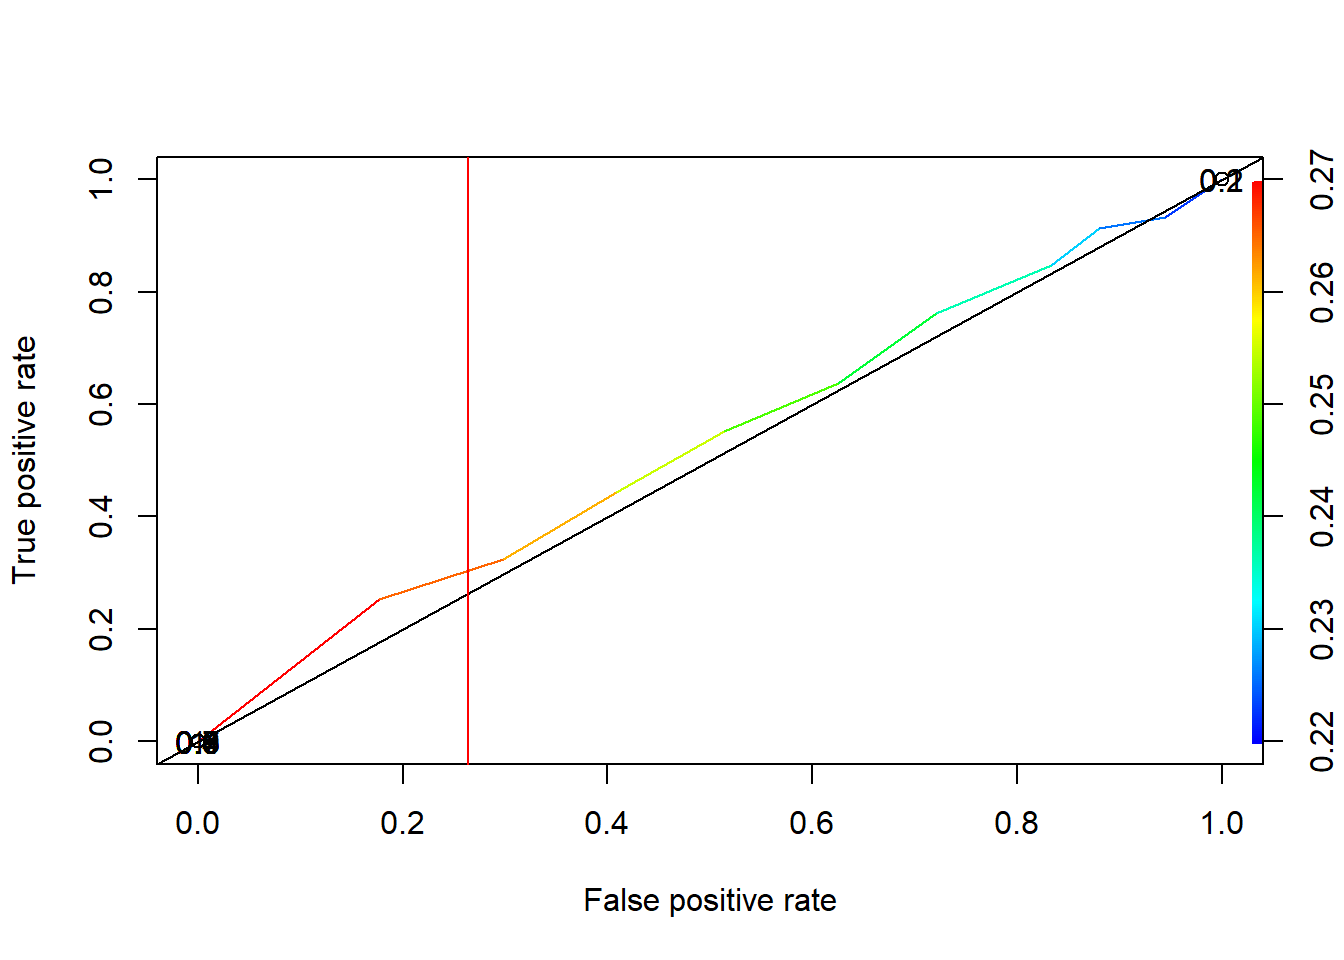
\includegraphics[width=0.9\linewidth]{bookdown-demo_files/figure-latex/unnamed-chunk-158-1} \caption{Punto de corte óptimo con datos tratados}\label{fig:unnamed-chunk-158}
\end{figure}

\textbf{Predicciones y matriz de confusión}

Se realizan predicciones y se genera una matriz de confusión.

\begin{example}
\protect\hypertarget{exm:bloque86nbm}{}\label{exm:bloque86nbm}Predicciones y matriz de confusión
\end{example}

\begin{Shaded}
\begin{Highlighting}[]
\NormalTok{pred.training}\OtherTok{\textless{}{-}}\FunctionTok{predict}\NormalTok{(modelo, }\AttributeTok{data=}\NormalTok{training, }\AttributeTok{type=}\StringTok{"response"}\NormalTok{)}
\FunctionTok{table}\NormalTok{(}\AttributeTok{ActualValue=}\NormalTok{training}\SpecialCharTok{$}\NormalTok{VP\_DC, }
      \AttributeTok{PredictValue=}\NormalTok{pred.training}\SpecialCharTok{\textgreater{}}\NormalTok{ptocorteop.training}\SpecialCharTok{$}\NormalTok{threshold)}
\end{Highlighting}
\end{Shaded}

\begin{verbatim}
##            PredictValue
## ActualValue FALSE TRUE
##           0  7778 1666
##           1  2292  774
\end{verbatim}

A continuación, se continua la evaluación del modelo con datos de prueba.

\textbf{Validación de modelo (con datos de prueba)}

Aplicamos nuevamente la validación con el test de Hosmer Lemeshow, esta vez con los datos de prueba.

\begin{example}
\protect\hypertarget{exm:bloque87nbm}{}\label{exm:bloque87nbm}Validación de modelo con datos de prueba
\end{example}

\begin{Shaded}
\begin{Highlighting}[]
\FunctionTok{hoslem.test}\NormalTok{(testing}\SpecialCharTok{$}\NormalTok{VP\_DC,}\FunctionTok{predict}\NormalTok{(modelo,}\AttributeTok{newdata=}\NormalTok{testing,}\AttributeTok{type=}\StringTok{"response"}\NormalTok{),}\AttributeTok{g=}\DecValTok{5}\NormalTok{)   }\CommentTok{\# Test de Hosmer Lemeshow}
\end{Highlighting}
\end{Shaded}

\begin{verbatim}
## 
##  Hosmer and Lemeshow goodness of fit (GOF) test
## 
## data:  testing$VP_DC, predict(modelo, newdata = testing, type = "response")
## X-squared = 66.467, df = 3, p-value = 2.431e-14
\end{verbatim}

\begin{Shaded}
\begin{Highlighting}[]
\NormalTok{indiceC.testing}\OtherTok{=}\FunctionTok{roc}\NormalTok{(testing}\SpecialCharTok{$}\NormalTok{VP\_DC,}\FunctionTok{predict}\NormalTok{(modelo,}\AttributeTok{newdata=}\NormalTok{testing,}\AttributeTok{type=}\StringTok{"response"}\NormalTok{)) }\CommentTok{\# Curva ROC}
\end{Highlighting}
\end{Shaded}

\begin{verbatim}
## Setting levels: control = 0, case = 1
\end{verbatim}

\begin{verbatim}
## Setting direction: controls < cases
\end{verbatim}

\begin{Shaded}
\begin{Highlighting}[]
\NormalTok{indiceC.testing}
\end{Highlighting}
\end{Shaded}

\begin{verbatim}
## 
## Call:
## roc.default(response = testing$VP_DC, predictor = predict(modelo,     newdata = testing, type = "response"))
## 
## Data: predict(modelo, newdata = testing, type = "response") in 4666 controls (testing$VP_DC 0) < 1590 cases (testing$VP_DC 1).
## Area under the curve: 0.5243
\end{verbatim}

\textbf{Punto de corte óptimo (con datos de prueba)}

Se calcula el punto de corte óptimo utilizando la función \texttt{coords()}.

\begin{example}
\protect\hypertarget{exm:bloque88nbm}{}\label{exm:bloque88nbm}Calcular de corte óptimo con datos de prueba
\end{example}

\begin{Shaded}
\begin{Highlighting}[]
\NormalTok{ptocorteop.testing}\OtherTok{\textless{}{-}}\FunctionTok{coords}\NormalTok{(indiceC.testing,}\AttributeTok{x=}\StringTok{"best"}\NormalTok{,}\AttributeTok{input=}\StringTok{"threshold"}\NormalTok{,}\AttributeTok{best.method=}\StringTok{"youden"}\NormalTok{)}
\NormalTok{ptocorteop.testing}
\end{Highlighting}
\end{Shaded}

\begin{verbatim}
##   threshold specificity sensitivity
## 1 0.2636494   0.8317617   0.2440252
\end{verbatim}

\begin{Shaded}
\begin{Highlighting}[]
\NormalTok{ROC.testing}\OtherTok{\textless{}{-}}\FunctionTok{performance}\NormalTok{(}\FunctionTok{prediction}\NormalTok{(}\FunctionTok{predict}\NormalTok{(modelo,}\AttributeTok{newdata=}\NormalTok{testing,}\AttributeTok{type=}\StringTok{"response"}\NormalTok{),}
                                    \FunctionTok{as.factor}\NormalTok{(testing}\SpecialCharTok{$}\NormalTok{VP\_DC)),}\StringTok{"tpr"}\NormalTok{,}\StringTok{"fpr"}\NormalTok{)}
\end{Highlighting}
\end{Shaded}

Luego, visualizamos el punto de corte óptimo utilizando la función \texttt{plot()}.

\begin{example}
\protect\hypertarget{exm:bloque89nbm}{}\label{exm:bloque89nbm}Visualizar de corte óptimo con datos de prueba
\end{example}

\begin{Shaded}
\begin{Highlighting}[]
\FunctionTok{plot}\NormalTok{(ROC.testing, }\AttributeTok{colorize=}\ConstantTok{TRUE}\NormalTok{, }\AttributeTok{print.cutoffs.at=}\FunctionTok{seq}\NormalTok{(}\FloatTok{0.1}\NormalTok{, }\AttributeTok{by=}\FloatTok{0.1}\NormalTok{))}
\FunctionTok{abline}\NormalTok{(}\AttributeTok{a=}\DecValTok{0}\NormalTok{,}\AttributeTok{b=}\DecValTok{1}\NormalTok{)}
\FunctionTok{abline}\NormalTok{(}\AttributeTok{v=}\NormalTok{ptocorteop.testing}\SpecialCharTok{$}\NormalTok{threshold,}\AttributeTok{col=}\StringTok{"red"}\NormalTok{)}
\end{Highlighting}
\end{Shaded}

\begin{figure}
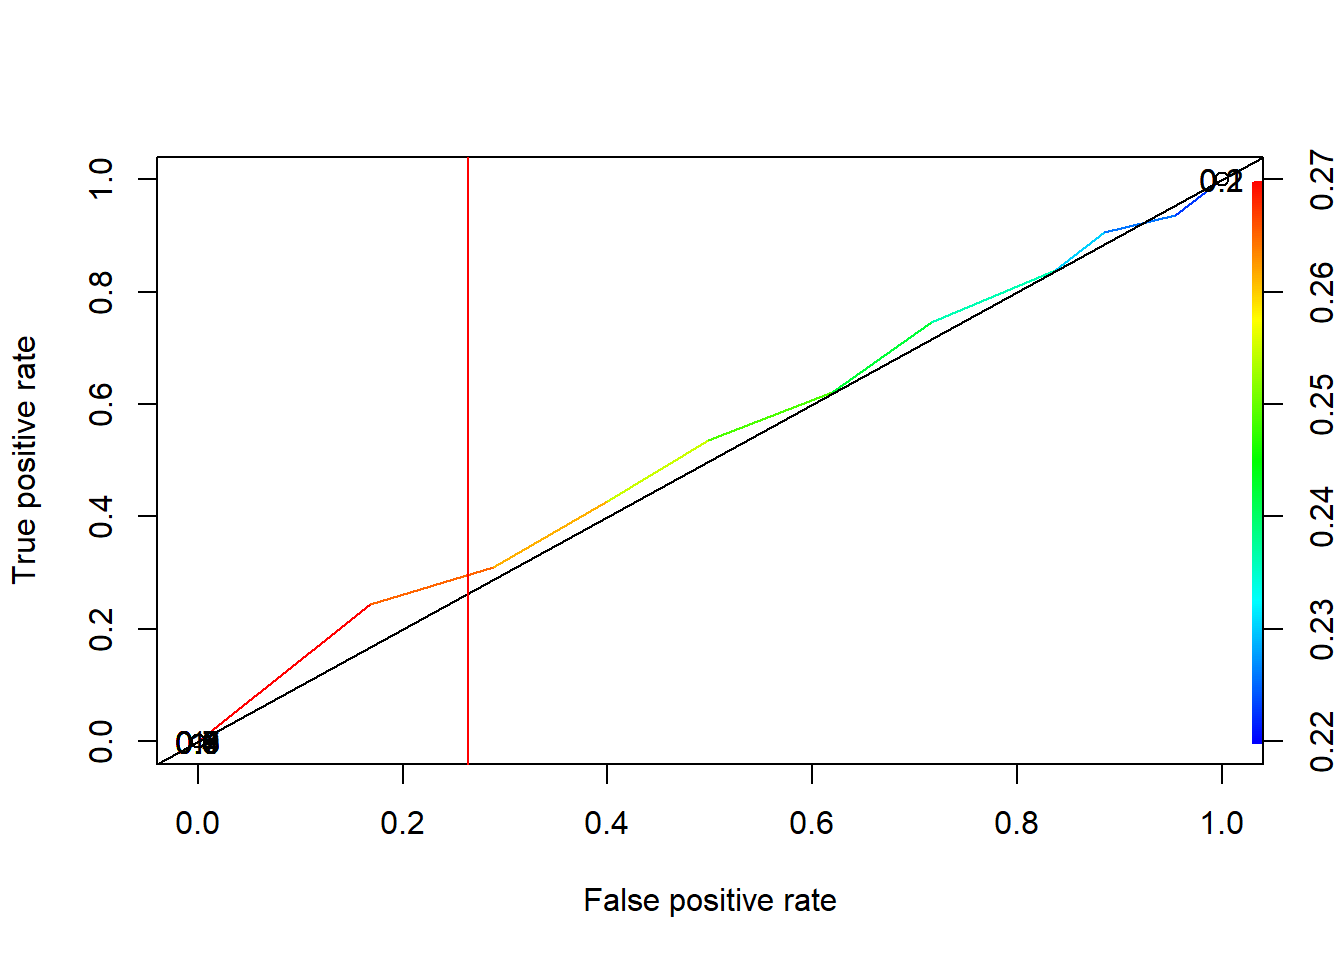
\includegraphics[width=0.9\linewidth]{bookdown-demo_files/figure-latex/unnamed-chunk-162-1} \caption{Punto de corte óptimo con datos de prueba a partir de datos tratados}\label{fig:unnamed-chunk-162}
\end{figure}

\textbf{Predicciones y matriz de confusión (con datos de prueba)}

Se realizan predicciones y se genera una matriz de confusión.

\begin{example}
\protect\hypertarget{exm:bloque90nbm}{}\label{exm:bloque90nbm}Predicciones y matriz de confusión con datos de prueba
\end{example}

\begin{Shaded}
\begin{Highlighting}[]
\NormalTok{pred.testing}\OtherTok{\textless{}{-}}\FunctionTok{predict}\NormalTok{(modelo, testing, }\AttributeTok{type=}\StringTok{"response"}\NormalTok{)}
\FunctionTok{table}\NormalTok{(}\AttributeTok{ActualValue=}\NormalTok{testing}\SpecialCharTok{$}\NormalTok{VP\_DC, }\AttributeTok{PredictValue=}\NormalTok{pred.testing}\SpecialCharTok{\textgreater{}}\NormalTok{ptocorteop.testing}\SpecialCharTok{$}\NormalTok{threshold)}
\end{Highlighting}
\end{Shaded}

\begin{verbatim}
##            PredictValue
## ActualValue FALSE TRUE
##           0  3881  785
##           1  1202  388
\end{verbatim}

\textbf{Compara área bajo la curva, umbral, sensibilidad y especificidad}

Finalmente, comparamos el área bajo la curva, umbral, sensibilidad y especificidad, a partir de los resultados del modelo con los datos de entrenamiento y con los datos de prueba.

\begin{example}
\protect\hypertarget{exm:bloque91nbm}{}\label{exm:bloque91nbm}Comparar área bajo la curva, umbral, sensibilidad y especificidad
\end{example}

\begin{Shaded}
\begin{Highlighting}[]
\NormalTok{auc    }\OtherTok{\textless{}{-}}\NormalTok{indiceC.trainig}\SpecialCharTok{$}\NormalTok{auc              }\SpecialCharTok{{-}}\NormalTok{ indiceC.testing}\SpecialCharTok{$}\NormalTok{auc}
\NormalTok{corte  }\OtherTok{\textless{}{-}}\NormalTok{ptocorteop.training}\SpecialCharTok{$}\NormalTok{threshold    }\SpecialCharTok{{-}}\NormalTok{ ptocorteop.testing}\SpecialCharTok{$}\NormalTok{threshold}
\NormalTok{sens   }\OtherTok{\textless{}{-}}\NormalTok{ ptocorteop.training}\SpecialCharTok{$}\NormalTok{sensitivity }\SpecialCharTok{{-}}\NormalTok{ ptocorteop.testing}\SpecialCharTok{$}\NormalTok{sensitivity}
\NormalTok{spe    }\OtherTok{\textless{}{-}}\NormalTok{ ptocorteop.training}\SpecialCharTok{$}\NormalTok{specificity }\SpecialCharTok{{-}}\NormalTok{ ptocorteop.testing}\SpecialCharTok{$}\NormalTok{specificity}
\end{Highlighting}
\end{Shaded}

La siguiente tabla muestra las estimaciones del coeficiente beta de la variable independiente de edad en los modelos, para los datos originales y los datos tratados. Se observa que ambas estimaciones son equivalentes, sin diferencias estadísticamente significativas a partir de su intervalo de confianza:

\begin{longtable}[]{@{}llll@{}}
\toprule()
Datos & Estimación & Lim. Inf. & Lim. Sup. \\
\midrule()
\endhead
Originales & 0,0035 & 0,0020 & 0,0050 \\
Tratados & 0,0036 & 0,0019 & 0,0053 \\
\bottomrule()
\end{longtable}

En suma, se observa que se mantienen las propiedades estadísticas priorizadas de la base de datos, por lo que cumple con las condiciones para su liberación.

\hypertarget{paso-seis-generar-reportes-y-liberar-datos}{%
\section{Paso Seis: Generar Reportes y Liberar Datos}\label{paso-seis-generar-reportes-y-liberar-datos}}

\hypertarget{reportes}{%
\subsection{Reportes}\label{reportes}}

Al realizar un ejercicio de anonimización como el recién expuesto, se debe elaborar un reporte que documente el proceso de anonimización, con sus antecedentes y resultados. Para ello, debe basarse en el modelo de reporte de anonimización descrito en la guía de anonimización.

\hypertarget{liberaciuxf3n-de-datos}{%
\subsection{Liberación de datos}\label{liberaciuxf3n-de-datos}}

A partir del objeto \emph{file}, que son los datos originales, se genera un objeto data.frame para su exportación como archivo de datos que será liberado.

Primero se verifica que el orden de registros sea idéntico entra datos originales y tratados. Esto permite sobre-escribir columnas completas, sabiendo que los registros coincidirán bien. En este caso, es importante usar el folio que corresponde a persona, ya que cada fila es una persona (en contraposición al folio de viviendas que cubre varias filas dependiendo de las personas que las componen).

\begin{example}
\protect\hypertarget{exm:bloque92nbm}{}\label{exm:bloque92nbm}Verificar coincidencia de folios
\end{example}

\begin{Shaded}
\begin{Highlighting}[]
\CommentTok{\# Se espera que esta función regrese TRUE}
\FunctionTok{all}\NormalTok{(file}\SpecialCharTok{$}\NormalTok{rph\_ID }\SpecialCharTok{==}\NormalTok{ fileTratada}\SpecialCharTok{$}\NormalTok{rph\_ID)}
\end{Highlighting}
\end{Shaded}

\begin{verbatim}
## [1] TRUE
\end{verbatim}

Luego, se reemplazan variables tratadas en datos originales y se eliminan las variables que están de más. Estas son, comuna y razón de inactividad, ya que esta última permitiría deshacer la recodificación que se realizó en la variable consolidada de situación ocupacional.

\begin{example}
\protect\hypertarget{exm:bloque93nbm}{}\label{exm:bloque93nbm}Eliminar variables
\end{example}

\begin{Shaded}
\begin{Highlighting}[]
\NormalTok{file}\SpecialCharTok{$}\NormalTok{enc\_rpc }\OtherTok{\textless{}{-}} \ConstantTok{NULL}
\NormalTok{file}\SpecialCharTok{$}\NormalTok{rph\_p14 }\OtherTok{\textless{}{-}} \ConstantTok{NULL}
\end{Highlighting}
\end{Shaded}

Luego, se reemplazan variables tratadas de edad, identidad de género, pertenencia indígena y nacionalidad.

\begin{example}
\protect\hypertarget{exm:bloque94nbm}{}\label{exm:bloque94nbm}Reemplazar variables originales por variables tratadas
\end{example}

\begin{Shaded}
\begin{Highlighting}[]
\NormalTok{file}\SpecialCharTok{$}\NormalTok{rph\_edad }\OtherTok{\textless{}{-}}\NormalTok{ fileTratada}\SpecialCharTok{$}\NormalTok{rph\_edad}
\NormalTok{file}\SpecialCharTok{$}\NormalTok{rph\_idgen }\OtherTok{\textless{}{-}}\NormalTok{ fileTratada}\SpecialCharTok{$}\NormalTok{rph\_idgen}
\NormalTok{file}\SpecialCharTok{$}\NormalTok{rph\_pertenencia\_indigena }\OtherTok{\textless{}{-}}\NormalTok{ fileTratada}\SpecialCharTok{$}\NormalTok{rph\_pertenencia\_indigena}
\NormalTok{file}\SpecialCharTok{$}\NormalTok{rph\_nacionalidad }\OtherTok{\textless{}{-}}\NormalTok{ fileTratada}\SpecialCharTok{$}\NormalTok{rph\_nacionalidad}
\end{Highlighting}
\end{Shaded}

Se eliminan los valores de rph\_p9 a rph\_p13 para los casos suprimidos en situación ocupacional

\begin{example}
\protect\hypertarget{exm:bloque95nbm}{}\label{exm:bloque95nbm}Suprimir valores
\end{example}

\begin{Shaded}
\begin{Highlighting}[]
\CommentTok{\# se eliminan los valores que corresponden}
\NormalTok{file}\SpecialCharTok{$}\NormalTok{rph\_p9[}\FunctionTok{is.na}\NormalTok{(fileTratada}\SpecialCharTok{$}\NormalTok{rph\_situacion\_ocupacional)] }\OtherTok{\textless{}{-}} \ConstantTok{NA}
\NormalTok{file}\SpecialCharTok{$}\NormalTok{rph\_p10[}\FunctionTok{is.na}\NormalTok{(fileTratada}\SpecialCharTok{$}\NormalTok{rph\_situacion\_ocupacional)] }\OtherTok{\textless{}{-}} \ConstantTok{NA}
\NormalTok{file}\SpecialCharTok{$}\NormalTok{rph\_p11[}\FunctionTok{is.na}\NormalTok{(fileTratada}\SpecialCharTok{$}\NormalTok{rph\_situacion\_ocupacional)] }\OtherTok{\textless{}{-}} \ConstantTok{NA}
\NormalTok{file}\SpecialCharTok{$}\NormalTok{rph\_p12[}\FunctionTok{is.na}\NormalTok{(fileTratada}\SpecialCharTok{$}\NormalTok{rph\_situacion\_ocupacional)] }\OtherTok{\textless{}{-}} \ConstantTok{NA}
\NormalTok{file}\SpecialCharTok{$}\NormalTok{rph\_p13[}\FunctionTok{is.na}\NormalTok{(fileTratada}\SpecialCharTok{$}\NormalTok{rph\_situacion\_ocupacional)] }\OtherTok{\textless{}{-}} \ConstantTok{NA}

\CommentTok{\# Luego eliminamos situación ocupacional ya que no se usará más}
\NormalTok{file}\SpecialCharTok{$}\NormalTok{rph\_situacion\_ocupacional }\OtherTok{\textless{}{-}} \ConstantTok{NULL}
\end{Highlighting}
\end{Shaded}

Luego, se elimina los valores de rph\_migración que son acompañados de un NA en nacionalidad, ya que sería un error de flujo de la encuesta mantenerlos.

\begin{example}
\protect\hypertarget{exm:bloque96nbm}{}\label{exm:bloque96nbm}Suprimir valores en nacionalidad
\end{example}

\begin{Shaded}
\begin{Highlighting}[]
\NormalTok{file}\SpecialCharTok{$}\NormalTok{rph\_migracion[}\FunctionTok{is.na}\NormalTok{(file}\SpecialCharTok{$}\NormalTok{rph\_nacionalidad)] }\OtherTok{\textless{}{-}} \ConstantTok{NA}
\end{Highlighting}
\end{Shaded}

Por último, se exporta archivo de datos ocupando la librería \texttt{haven}.

\begin{example}
\protect\hypertarget{exm:bloque97nbm}{}\label{exm:bloque97nbm}Ejemplo de código para exportar datos anonimizados
\end{example}

\begin{Shaded}
\begin{Highlighting}[]
\CommentTok{\#haven::write\_sav(file, \textquotesingle{}ENUSC2020\_anonimizada.sav\textquotesingle{})}
\end{Highlighting}
\end{Shaded}

\hypertarget{anexo-tablas-de-indicadores-con-desagregaciones}{%
\subsection{Anexo : Tablas de indicadores con desagregaciones}\label{anexo-tablas-de-indicadores-con-desagregaciones}}

Se deja como anexo los tabulados con datos tratados y no tratados por si se considera necesario compararlos de forma manual.

\begin{example}
\protect\hypertarget{exm:bloque98nbm}{}\label{exm:bloque98nbm}Ejemplo de código para exportar datos de indicadores con datos tratados y no tratados
\end{example}

\begin{Shaded}
\begin{Highlighting}[]
\CommentTok{\#anexo \textless{}{-} list(\textquotesingle{}P1 Regional Original\textquotesingle{} = P1\_REG\_PRE,}
\CommentTok{\#              \textquotesingle{}P1 Regional Tratado\textquotesingle{} = P1\_REG\_TRAT,}
\CommentTok{\#              \textquotesingle{}P1 Sexo Original\textquotesingle{} = P1\_SEXO\_PRE,}
\CommentTok{\#              \textquotesingle{}P1 Sexo Tratado\textquotesingle{} = P1\_SEXO\_TRAT,}
\CommentTok{\#              \textquotesingle{}P1 Regional Sexo Original\textquotesingle{} = P1\_REG\_SEXO\_PRE,}
\CommentTok{\#              \textquotesingle{}P1 Regional Sexo Tratado\textquotesingle{} = P1\_REG\_SEXO\_TRAT,}
\CommentTok{\#              \textquotesingle{}Vict. Pers. Regional Original\textquotesingle{} = VP\_DC\_REG\_PRE,}
\CommentTok{\#              \textquotesingle{}Vict. Pers. Regional Tratado\textquotesingle{} = VP\_DC\_REG\_TRAT,}
\CommentTok{\#              \textquotesingle{}Vict. Pers. Sexo Original\textquotesingle{} = VP\_DC\_SEXO\_PRE,}
\CommentTok{\#              \textquotesingle{}Vict. Pers. Sexo Tratado\textquotesingle{} = VP\_DC\_SEXO\_TRAT,}
\CommentTok{\#              \textquotesingle{}Vict. Pers. Regional Sexo Original\textquotesingle{} = VP\_DC\_REG\_SEXO\_PRE,}
\CommentTok{\#              \textquotesingle{}Vict. Pers. Regional Sexo Tratado\textquotesingle{} = VP\_DC\_REG\_SEXO\_TRAT,}
\CommentTok{\#              \textquotesingle{}Vict. Agr. Regional Original\textquotesingle{} = VA\_DC\_REG\_PRE,}
\CommentTok{\#              \textquotesingle{}Vict. Agr. Regional Tratado\textquotesingle{} = VA\_DC\_REG\_TRAT)}
\CommentTok{\#}
\CommentTok{\#openxlsx::write.xlsx(anexo, "Anexo\_Medicion\_Utilidad.xlsx")}
\end{Highlighting}
\end{Shaded}

\hypertarget{taller-sdc-video}{%
\chapter{Taller SDC Video}\label{taller-sdc-video}}

El Instituto Nacional de Estadísticas (INE) realizó el 14 de abril de 2021 el ``Taller sobre proceso de control a la divulgación estadística en microdatos, INE 2021''. El objetivo principal del taller fue revisar aspectos teóricos y prácticos del control a la divulgación estadística en microdatos (SDC, por su sigla en inglés), abordando motivaciones técnicas para su aplicación, sus etapas, beneficios y áreas de atención, entre otros puntos claves.

El taller fue liderado por el analista estadístico Julio Guerrero Rojas y el analista socioeconómico Nicolás Berho Montalvo, del DMIE y la Subdirección Técnica (SDT), respectivamente.

En la primera parte del taller, los expositores presentaron una introducción al SDC, destacando su importancia para garantizar la confidencialidad y privacidad de los datos personales en la difusión de microdatos.

En la segunda parte, los expositores abordaron las motivaciones técnicas para la aplicación del SDC, así como sus etapas, beneficios y áreas de atención.

En la tercera parte, los asistentes tuvieron la oportunidad de realizar preguntas y comentarios.

Dejamos en video de la experiencia:

  \bibliography{references.bib,packages.bib}

\end{document}
